\subsection{Benchmark: Lorenz 1963}

We first verified that our choice of implementation for \glspl{esn}
produces similar results to those found in the literature \cite{pathak_using_2017}.
\begin{figure*}[t]
  % 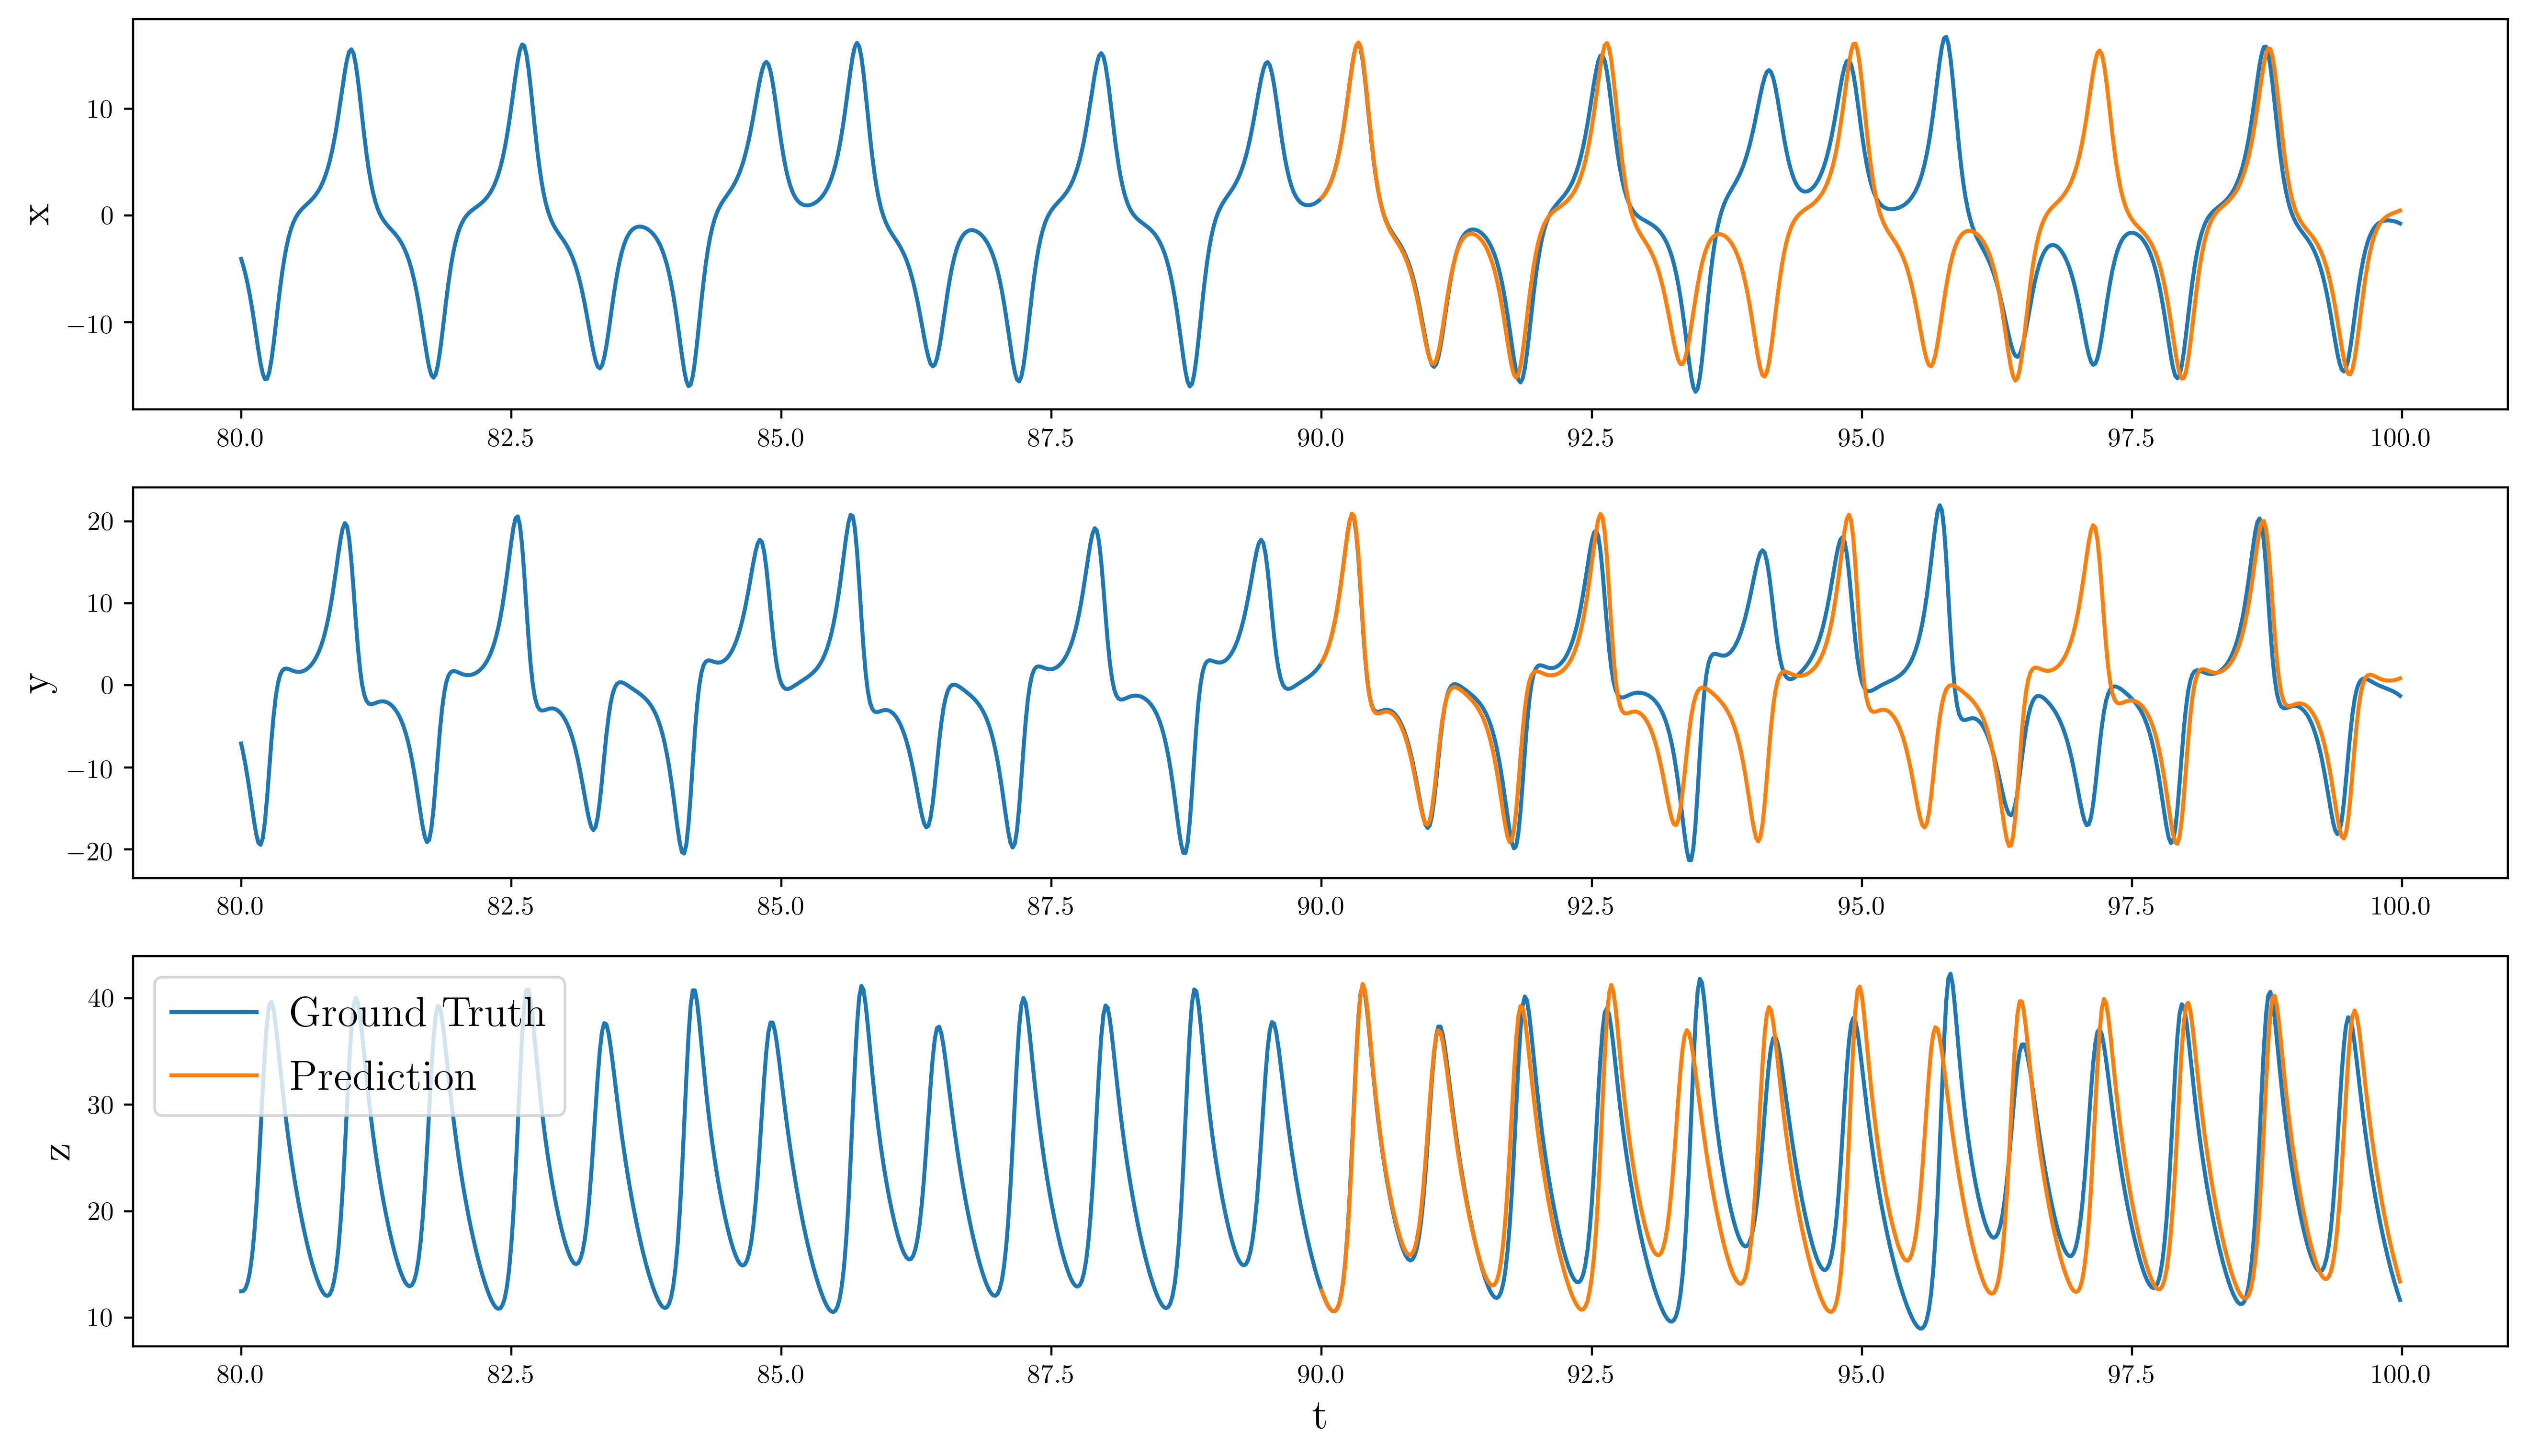
\includegraphics[width=\columnwidth]{lorenz63_prediction.png}
  %% Creator: Matplotlib, PGF backend
%%
%% To include the figure in your LaTeX document, write
%%   \input{<filename>.pgf}
%%
%% Make sure the required packages are loaded in your preamble
%%   \usepackage{pgf}
%%
%% Figures using additional raster images can only be included by \input if
%% they are in the same directory as the main LaTeX file. For loading figures
%% from other directories you can use the `import` package
%%   \usepackage{import}
%% and then include the figures with
%%   \import{<path to file>}{<filename>.pgf}
%%
%% Matplotlib used the following preamble
%%
\begingroup%
\makeatletter%
\begin{pgfpicture}%
\pgfpathrectangle{\pgfpointorigin}{\pgfqpoint{5.575292in}{4.947957in}}%
\pgfusepath{use as bounding box, clip}%
\begin{pgfscope}%
\pgfsetbuttcap%
\pgfsetmiterjoin%
\definecolor{currentfill}{rgb}{1.000000,1.000000,1.000000}%
\pgfsetfillcolor{currentfill}%
\pgfsetlinewidth{0.000000pt}%
\definecolor{currentstroke}{rgb}{1.000000,1.000000,1.000000}%
\pgfsetstrokecolor{currentstroke}%
\pgfsetdash{}{0pt}%
\pgfpathmoveto{\pgfqpoint{0.000000in}{0.000000in}}%
\pgfpathlineto{\pgfqpoint{5.575292in}{0.000000in}}%
\pgfpathlineto{\pgfqpoint{5.575292in}{4.947957in}}%
\pgfpathlineto{\pgfqpoint{0.000000in}{4.947957in}}%
\pgfpathclose%
\pgfusepath{fill}%
\end{pgfscope}%
\begin{pgfscope}%
\pgfsetbuttcap%
\pgfsetmiterjoin%
\definecolor{currentfill}{rgb}{1.000000,1.000000,1.000000}%
\pgfsetfillcolor{currentfill}%
\pgfsetlinewidth{0.000000pt}%
\definecolor{currentstroke}{rgb}{0.000000,0.000000,0.000000}%
\pgfsetstrokecolor{currentstroke}%
\pgfsetstrokeopacity{0.000000}%
\pgfsetdash{}{0pt}%
\pgfpathmoveto{\pgfqpoint{0.713041in}{3.595494in}}%
\pgfpathlineto{\pgfqpoint{5.475292in}{3.595494in}}%
\pgfpathlineto{\pgfqpoint{5.475292in}{4.847957in}}%
\pgfpathlineto{\pgfqpoint{0.713041in}{4.847957in}}%
\pgfpathclose%
\pgfusepath{fill}%
\end{pgfscope}%
\begin{pgfscope}%
\pgfsetbuttcap%
\pgfsetroundjoin%
\definecolor{currentfill}{rgb}{0.000000,0.000000,0.000000}%
\pgfsetfillcolor{currentfill}%
\pgfsetlinewidth{0.803000pt}%
\definecolor{currentstroke}{rgb}{0.000000,0.000000,0.000000}%
\pgfsetstrokecolor{currentstroke}%
\pgfsetdash{}{0pt}%
\pgfsys@defobject{currentmarker}{\pgfqpoint{0.000000in}{-0.048611in}}{\pgfqpoint{0.000000in}{0.000000in}}{%
\pgfpathmoveto{\pgfqpoint{0.000000in}{0.000000in}}%
\pgfpathlineto{\pgfqpoint{0.000000in}{-0.048611in}}%
\pgfusepath{stroke,fill}%
}%
\begin{pgfscope}%
\pgfsys@transformshift{0.929507in}{3.595494in}%
\pgfsys@useobject{currentmarker}{}%
\end{pgfscope}%
\end{pgfscope}%
\begin{pgfscope}%
\definecolor{textcolor}{rgb}{0.000000,0.000000,0.000000}%
\pgfsetstrokecolor{textcolor}%
\pgfsetfillcolor{textcolor}%
\pgftext[x=0.929507in,y=3.498272in,,top]{\color{textcolor}\rmfamily\fontsize{10.000000}{12.000000}\selectfont \(\displaystyle 80.0\)}%
\end{pgfscope}%
\begin{pgfscope}%
\pgfsetbuttcap%
\pgfsetroundjoin%
\definecolor{currentfill}{rgb}{0.000000,0.000000,0.000000}%
\pgfsetfillcolor{currentfill}%
\pgfsetlinewidth{0.803000pt}%
\definecolor{currentstroke}{rgb}{0.000000,0.000000,0.000000}%
\pgfsetstrokecolor{currentstroke}%
\pgfsetdash{}{0pt}%
\pgfsys@defobject{currentmarker}{\pgfqpoint{0.000000in}{-0.048611in}}{\pgfqpoint{0.000000in}{0.000000in}}{%
\pgfpathmoveto{\pgfqpoint{0.000000in}{0.000000in}}%
\pgfpathlineto{\pgfqpoint{0.000000in}{-0.048611in}}%
\pgfusepath{stroke,fill}%
}%
\begin{pgfscope}%
\pgfsys@transformshift{1.471213in}{3.595494in}%
\pgfsys@useobject{currentmarker}{}%
\end{pgfscope}%
\end{pgfscope}%
\begin{pgfscope}%
\definecolor{textcolor}{rgb}{0.000000,0.000000,0.000000}%
\pgfsetstrokecolor{textcolor}%
\pgfsetfillcolor{textcolor}%
\pgftext[x=1.471213in,y=3.498272in,,top]{\color{textcolor}\rmfamily\fontsize{10.000000}{12.000000}\selectfont \(\displaystyle 82.5\)}%
\end{pgfscope}%
\begin{pgfscope}%
\pgfsetbuttcap%
\pgfsetroundjoin%
\definecolor{currentfill}{rgb}{0.000000,0.000000,0.000000}%
\pgfsetfillcolor{currentfill}%
\pgfsetlinewidth{0.803000pt}%
\definecolor{currentstroke}{rgb}{0.000000,0.000000,0.000000}%
\pgfsetstrokecolor{currentstroke}%
\pgfsetdash{}{0pt}%
\pgfsys@defobject{currentmarker}{\pgfqpoint{0.000000in}{-0.048611in}}{\pgfqpoint{0.000000in}{0.000000in}}{%
\pgfpathmoveto{\pgfqpoint{0.000000in}{0.000000in}}%
\pgfpathlineto{\pgfqpoint{0.000000in}{-0.048611in}}%
\pgfusepath{stroke,fill}%
}%
\begin{pgfscope}%
\pgfsys@transformshift{2.012920in}{3.595494in}%
\pgfsys@useobject{currentmarker}{}%
\end{pgfscope}%
\end{pgfscope}%
\begin{pgfscope}%
\definecolor{textcolor}{rgb}{0.000000,0.000000,0.000000}%
\pgfsetstrokecolor{textcolor}%
\pgfsetfillcolor{textcolor}%
\pgftext[x=2.012920in,y=3.498272in,,top]{\color{textcolor}\rmfamily\fontsize{10.000000}{12.000000}\selectfont \(\displaystyle 85.0\)}%
\end{pgfscope}%
\begin{pgfscope}%
\pgfsetbuttcap%
\pgfsetroundjoin%
\definecolor{currentfill}{rgb}{0.000000,0.000000,0.000000}%
\pgfsetfillcolor{currentfill}%
\pgfsetlinewidth{0.803000pt}%
\definecolor{currentstroke}{rgb}{0.000000,0.000000,0.000000}%
\pgfsetstrokecolor{currentstroke}%
\pgfsetdash{}{0pt}%
\pgfsys@defobject{currentmarker}{\pgfqpoint{0.000000in}{-0.048611in}}{\pgfqpoint{0.000000in}{0.000000in}}{%
\pgfpathmoveto{\pgfqpoint{0.000000in}{0.000000in}}%
\pgfpathlineto{\pgfqpoint{0.000000in}{-0.048611in}}%
\pgfusepath{stroke,fill}%
}%
\begin{pgfscope}%
\pgfsys@transformshift{2.554626in}{3.595494in}%
\pgfsys@useobject{currentmarker}{}%
\end{pgfscope}%
\end{pgfscope}%
\begin{pgfscope}%
\definecolor{textcolor}{rgb}{0.000000,0.000000,0.000000}%
\pgfsetstrokecolor{textcolor}%
\pgfsetfillcolor{textcolor}%
\pgftext[x=2.554626in,y=3.498272in,,top]{\color{textcolor}\rmfamily\fontsize{10.000000}{12.000000}\selectfont \(\displaystyle 87.5\)}%
\end{pgfscope}%
\begin{pgfscope}%
\pgfsetbuttcap%
\pgfsetroundjoin%
\definecolor{currentfill}{rgb}{0.000000,0.000000,0.000000}%
\pgfsetfillcolor{currentfill}%
\pgfsetlinewidth{0.803000pt}%
\definecolor{currentstroke}{rgb}{0.000000,0.000000,0.000000}%
\pgfsetstrokecolor{currentstroke}%
\pgfsetdash{}{0pt}%
\pgfsys@defobject{currentmarker}{\pgfqpoint{0.000000in}{-0.048611in}}{\pgfqpoint{0.000000in}{0.000000in}}{%
\pgfpathmoveto{\pgfqpoint{0.000000in}{0.000000in}}%
\pgfpathlineto{\pgfqpoint{0.000000in}{-0.048611in}}%
\pgfusepath{stroke,fill}%
}%
\begin{pgfscope}%
\pgfsys@transformshift{3.096333in}{3.595494in}%
\pgfsys@useobject{currentmarker}{}%
\end{pgfscope}%
\end{pgfscope}%
\begin{pgfscope}%
\definecolor{textcolor}{rgb}{0.000000,0.000000,0.000000}%
\pgfsetstrokecolor{textcolor}%
\pgfsetfillcolor{textcolor}%
\pgftext[x=3.096333in,y=3.498272in,,top]{\color{textcolor}\rmfamily\fontsize{10.000000}{12.000000}\selectfont \(\displaystyle 90.0\)}%
\end{pgfscope}%
\begin{pgfscope}%
\pgfsetbuttcap%
\pgfsetroundjoin%
\definecolor{currentfill}{rgb}{0.000000,0.000000,0.000000}%
\pgfsetfillcolor{currentfill}%
\pgfsetlinewidth{0.803000pt}%
\definecolor{currentstroke}{rgb}{0.000000,0.000000,0.000000}%
\pgfsetstrokecolor{currentstroke}%
\pgfsetdash{}{0pt}%
\pgfsys@defobject{currentmarker}{\pgfqpoint{0.000000in}{-0.048611in}}{\pgfqpoint{0.000000in}{0.000000in}}{%
\pgfpathmoveto{\pgfqpoint{0.000000in}{0.000000in}}%
\pgfpathlineto{\pgfqpoint{0.000000in}{-0.048611in}}%
\pgfusepath{stroke,fill}%
}%
\begin{pgfscope}%
\pgfsys@transformshift{3.638040in}{3.595494in}%
\pgfsys@useobject{currentmarker}{}%
\end{pgfscope}%
\end{pgfscope}%
\begin{pgfscope}%
\definecolor{textcolor}{rgb}{0.000000,0.000000,0.000000}%
\pgfsetstrokecolor{textcolor}%
\pgfsetfillcolor{textcolor}%
\pgftext[x=3.638040in,y=3.498272in,,top]{\color{textcolor}\rmfamily\fontsize{10.000000}{12.000000}\selectfont \(\displaystyle 92.5\)}%
\end{pgfscope}%
\begin{pgfscope}%
\pgfsetbuttcap%
\pgfsetroundjoin%
\definecolor{currentfill}{rgb}{0.000000,0.000000,0.000000}%
\pgfsetfillcolor{currentfill}%
\pgfsetlinewidth{0.803000pt}%
\definecolor{currentstroke}{rgb}{0.000000,0.000000,0.000000}%
\pgfsetstrokecolor{currentstroke}%
\pgfsetdash{}{0pt}%
\pgfsys@defobject{currentmarker}{\pgfqpoint{0.000000in}{-0.048611in}}{\pgfqpoint{0.000000in}{0.000000in}}{%
\pgfpathmoveto{\pgfqpoint{0.000000in}{0.000000in}}%
\pgfpathlineto{\pgfqpoint{0.000000in}{-0.048611in}}%
\pgfusepath{stroke,fill}%
}%
\begin{pgfscope}%
\pgfsys@transformshift{4.179746in}{3.595494in}%
\pgfsys@useobject{currentmarker}{}%
\end{pgfscope}%
\end{pgfscope}%
\begin{pgfscope}%
\definecolor{textcolor}{rgb}{0.000000,0.000000,0.000000}%
\pgfsetstrokecolor{textcolor}%
\pgfsetfillcolor{textcolor}%
\pgftext[x=4.179746in,y=3.498272in,,top]{\color{textcolor}\rmfamily\fontsize{10.000000}{12.000000}\selectfont \(\displaystyle 95.0\)}%
\end{pgfscope}%
\begin{pgfscope}%
\pgfsetbuttcap%
\pgfsetroundjoin%
\definecolor{currentfill}{rgb}{0.000000,0.000000,0.000000}%
\pgfsetfillcolor{currentfill}%
\pgfsetlinewidth{0.803000pt}%
\definecolor{currentstroke}{rgb}{0.000000,0.000000,0.000000}%
\pgfsetstrokecolor{currentstroke}%
\pgfsetdash{}{0pt}%
\pgfsys@defobject{currentmarker}{\pgfqpoint{0.000000in}{-0.048611in}}{\pgfqpoint{0.000000in}{0.000000in}}{%
\pgfpathmoveto{\pgfqpoint{0.000000in}{0.000000in}}%
\pgfpathlineto{\pgfqpoint{0.000000in}{-0.048611in}}%
\pgfusepath{stroke,fill}%
}%
\begin{pgfscope}%
\pgfsys@transformshift{4.721453in}{3.595494in}%
\pgfsys@useobject{currentmarker}{}%
\end{pgfscope}%
\end{pgfscope}%
\begin{pgfscope}%
\definecolor{textcolor}{rgb}{0.000000,0.000000,0.000000}%
\pgfsetstrokecolor{textcolor}%
\pgfsetfillcolor{textcolor}%
\pgftext[x=4.721453in,y=3.498272in,,top]{\color{textcolor}\rmfamily\fontsize{10.000000}{12.000000}\selectfont \(\displaystyle 97.5\)}%
\end{pgfscope}%
\begin{pgfscope}%
\pgfsetbuttcap%
\pgfsetroundjoin%
\definecolor{currentfill}{rgb}{0.000000,0.000000,0.000000}%
\pgfsetfillcolor{currentfill}%
\pgfsetlinewidth{0.803000pt}%
\definecolor{currentstroke}{rgb}{0.000000,0.000000,0.000000}%
\pgfsetstrokecolor{currentstroke}%
\pgfsetdash{}{0pt}%
\pgfsys@defobject{currentmarker}{\pgfqpoint{0.000000in}{-0.048611in}}{\pgfqpoint{0.000000in}{0.000000in}}{%
\pgfpathmoveto{\pgfqpoint{0.000000in}{0.000000in}}%
\pgfpathlineto{\pgfqpoint{0.000000in}{-0.048611in}}%
\pgfusepath{stroke,fill}%
}%
\begin{pgfscope}%
\pgfsys@transformshift{5.263159in}{3.595494in}%
\pgfsys@useobject{currentmarker}{}%
\end{pgfscope}%
\end{pgfscope}%
\begin{pgfscope}%
\definecolor{textcolor}{rgb}{0.000000,0.000000,0.000000}%
\pgfsetstrokecolor{textcolor}%
\pgfsetfillcolor{textcolor}%
\pgftext[x=5.263159in,y=3.498272in,,top]{\color{textcolor}\rmfamily\fontsize{10.000000}{12.000000}\selectfont \(\displaystyle 100.0\)}%
\end{pgfscope}%
\begin{pgfscope}%
\pgfsetbuttcap%
\pgfsetroundjoin%
\definecolor{currentfill}{rgb}{0.000000,0.000000,0.000000}%
\pgfsetfillcolor{currentfill}%
\pgfsetlinewidth{0.803000pt}%
\definecolor{currentstroke}{rgb}{0.000000,0.000000,0.000000}%
\pgfsetstrokecolor{currentstroke}%
\pgfsetdash{}{0pt}%
\pgfsys@defobject{currentmarker}{\pgfqpoint{-0.048611in}{0.000000in}}{\pgfqpoint{0.000000in}{0.000000in}}{%
\pgfpathmoveto{\pgfqpoint{0.000000in}{0.000000in}}%
\pgfpathlineto{\pgfqpoint{-0.048611in}{0.000000in}}%
\pgfusepath{stroke,fill}%
}%
\begin{pgfscope}%
\pgfsys@transformshift{0.713041in}{3.876040in}%
\pgfsys@useobject{currentmarker}{}%
\end{pgfscope}%
\end{pgfscope}%
\begin{pgfscope}%
\definecolor{textcolor}{rgb}{0.000000,0.000000,0.000000}%
\pgfsetstrokecolor{textcolor}%
\pgfsetfillcolor{textcolor}%
\pgftext[x=0.368904in,y=3.827814in,left,base]{\color{textcolor}\rmfamily\fontsize{10.000000}{12.000000}\selectfont \(\displaystyle -10\)}%
\end{pgfscope}%
\begin{pgfscope}%
\pgfsetbuttcap%
\pgfsetroundjoin%
\definecolor{currentfill}{rgb}{0.000000,0.000000,0.000000}%
\pgfsetfillcolor{currentfill}%
\pgfsetlinewidth{0.803000pt}%
\definecolor{currentstroke}{rgb}{0.000000,0.000000,0.000000}%
\pgfsetstrokecolor{currentstroke}%
\pgfsetdash{}{0pt}%
\pgfsys@defobject{currentmarker}{\pgfqpoint{-0.048611in}{0.000000in}}{\pgfqpoint{0.000000in}{0.000000in}}{%
\pgfpathmoveto{\pgfqpoint{0.000000in}{0.000000in}}%
\pgfpathlineto{\pgfqpoint{-0.048611in}{0.000000in}}%
\pgfusepath{stroke,fill}%
}%
\begin{pgfscope}%
\pgfsys@transformshift{0.713041in}{4.218055in}%
\pgfsys@useobject{currentmarker}{}%
\end{pgfscope}%
\end{pgfscope}%
\begin{pgfscope}%
\definecolor{textcolor}{rgb}{0.000000,0.000000,0.000000}%
\pgfsetstrokecolor{textcolor}%
\pgfsetfillcolor{textcolor}%
\pgftext[x=0.546374in,y=4.169830in,left,base]{\color{textcolor}\rmfamily\fontsize{10.000000}{12.000000}\selectfont \(\displaystyle 0\)}%
\end{pgfscope}%
\begin{pgfscope}%
\pgfsetbuttcap%
\pgfsetroundjoin%
\definecolor{currentfill}{rgb}{0.000000,0.000000,0.000000}%
\pgfsetfillcolor{currentfill}%
\pgfsetlinewidth{0.803000pt}%
\definecolor{currentstroke}{rgb}{0.000000,0.000000,0.000000}%
\pgfsetstrokecolor{currentstroke}%
\pgfsetdash{}{0pt}%
\pgfsys@defobject{currentmarker}{\pgfqpoint{-0.048611in}{0.000000in}}{\pgfqpoint{0.000000in}{0.000000in}}{%
\pgfpathmoveto{\pgfqpoint{0.000000in}{0.000000in}}%
\pgfpathlineto{\pgfqpoint{-0.048611in}{0.000000in}}%
\pgfusepath{stroke,fill}%
}%
\begin{pgfscope}%
\pgfsys@transformshift{0.713041in}{4.560070in}%
\pgfsys@useobject{currentmarker}{}%
\end{pgfscope}%
\end{pgfscope}%
\begin{pgfscope}%
\definecolor{textcolor}{rgb}{0.000000,0.000000,0.000000}%
\pgfsetstrokecolor{textcolor}%
\pgfsetfillcolor{textcolor}%
\pgftext[x=0.476929in,y=4.511845in,left,base]{\color{textcolor}\rmfamily\fontsize{10.000000}{12.000000}\selectfont \(\displaystyle 10\)}%
\end{pgfscope}%
\begin{pgfscope}%
\definecolor{textcolor}{rgb}{0.000000,0.000000,0.000000}%
\pgfsetstrokecolor{textcolor}%
\pgfsetfillcolor{textcolor}%
\pgftext[x=0.313349in,y=4.221726in,,bottom,rotate=90.000000]{\color{textcolor}\rmfamily\fontsize{16.000000}{19.200000}\selectfont x}%
\end{pgfscope}%
\begin{pgfscope}%
\pgfpathrectangle{\pgfqpoint{0.713041in}{3.595494in}}{\pgfqpoint{4.762251in}{1.252463in}}%
\pgfusepath{clip}%
\pgfsetrectcap%
\pgfsetroundjoin%
\pgfsetlinewidth{1.505625pt}%
\definecolor{currentstroke}{rgb}{0.121569,0.466667,0.705882}%
\pgfsetstrokecolor{currentstroke}%
\pgfsetdash{}{0pt}%
\pgfpathmoveto{\pgfqpoint{0.929507in}{4.078618in}}%
\pgfpathlineto{\pgfqpoint{0.933840in}{4.056045in}}%
\pgfpathlineto{\pgfqpoint{0.938174in}{4.029465in}}%
\pgfpathlineto{\pgfqpoint{0.942508in}{3.998463in}}%
\pgfpathlineto{\pgfqpoint{0.946841in}{3.962786in}}%
\pgfpathlineto{\pgfqpoint{0.951175in}{3.922509in}}%
\pgfpathlineto{\pgfqpoint{0.959842in}{3.831645in}}%
\pgfpathlineto{\pgfqpoint{0.964176in}{3.785316in}}%
\pgfpathlineto{\pgfqpoint{0.968510in}{3.743339in}}%
\pgfpathlineto{\pgfqpoint{0.972843in}{3.710807in}}%
\pgfpathlineto{\pgfqpoint{0.977177in}{3.692969in}}%
\pgfpathlineto{\pgfqpoint{0.981510in}{3.693813in}}%
\pgfpathlineto{\pgfqpoint{0.985844in}{3.714648in}}%
\pgfpathlineto{\pgfqpoint{0.990178in}{3.753477in}}%
\pgfpathlineto{\pgfqpoint{0.994511in}{3.805567in}}%
\pgfpathlineto{\pgfqpoint{1.007512in}{3.983613in}}%
\pgfpathlineto{\pgfqpoint{1.011846in}{4.035694in}}%
\pgfpathlineto{\pgfqpoint{1.016180in}{4.080624in}}%
\pgfpathlineto{\pgfqpoint{1.020513in}{4.118151in}}%
\pgfpathlineto{\pgfqpoint{1.024847in}{4.148733in}}%
\pgfpathlineto{\pgfqpoint{1.029181in}{4.173212in}}%
\pgfpathlineto{\pgfqpoint{1.033514in}{4.192584in}}%
\pgfpathlineto{\pgfqpoint{1.037848in}{4.207857in}}%
\pgfpathlineto{\pgfqpoint{1.042182in}{4.219961in}}%
\pgfpathlineto{\pgfqpoint{1.046515in}{4.229721in}}%
\pgfpathlineto{\pgfqpoint{1.050849in}{4.237840in}}%
\pgfpathlineto{\pgfqpoint{1.055183in}{4.244911in}}%
\pgfpathlineto{\pgfqpoint{1.068184in}{4.264457in}}%
\pgfpathlineto{\pgfqpoint{1.072517in}{4.271672in}}%
\pgfpathlineto{\pgfqpoint{1.076851in}{4.279791in}}%
\pgfpathlineto{\pgfqpoint{1.081184in}{4.289139in}}%
\pgfpathlineto{\pgfqpoint{1.085518in}{4.300060in}}%
\pgfpathlineto{\pgfqpoint{1.089852in}{4.312931in}}%
\pgfpathlineto{\pgfqpoint{1.094185in}{4.328164in}}%
\pgfpathlineto{\pgfqpoint{1.098519in}{4.346220in}}%
\pgfpathlineto{\pgfqpoint{1.102853in}{4.367598in}}%
\pgfpathlineto{\pgfqpoint{1.107186in}{4.392817in}}%
\pgfpathlineto{\pgfqpoint{1.111520in}{4.422369in}}%
\pgfpathlineto{\pgfqpoint{1.115854in}{4.456640in}}%
\pgfpathlineto{\pgfqpoint{1.120187in}{4.495760in}}%
\pgfpathlineto{\pgfqpoint{1.124521in}{4.539383in}}%
\pgfpathlineto{\pgfqpoint{1.137522in}{4.680195in}}%
\pgfpathlineto{\pgfqpoint{1.141856in}{4.718444in}}%
\pgfpathlineto{\pgfqpoint{1.146189in}{4.743676in}}%
\pgfpathlineto{\pgfqpoint{1.150523in}{4.750947in}}%
\pgfpathlineto{\pgfqpoint{1.154857in}{4.737582in}}%
\pgfpathlineto{\pgfqpoint{1.159190in}{4.704298in}}%
\pgfpathlineto{\pgfqpoint{1.163524in}{4.655093in}}%
\pgfpathlineto{\pgfqpoint{1.172191in}{4.533238in}}%
\pgfpathlineto{\pgfqpoint{1.176525in}{4.472108in}}%
\pgfpathlineto{\pgfqpoint{1.180859in}{4.416143in}}%
\pgfpathlineto{\pgfqpoint{1.185192in}{4.367247in}}%
\pgfpathlineto{\pgfqpoint{1.189526in}{4.326012in}}%
\pgfpathlineto{\pgfqpoint{1.193859in}{4.292155in}}%
\pgfpathlineto{\pgfqpoint{1.198193in}{4.264887in}}%
\pgfpathlineto{\pgfqpoint{1.202527in}{4.243190in}}%
\pgfpathlineto{\pgfqpoint{1.206860in}{4.225998in}}%
\pgfpathlineto{\pgfqpoint{1.211194in}{4.212301in}}%
\pgfpathlineto{\pgfqpoint{1.215528in}{4.201195in}}%
\pgfpathlineto{\pgfqpoint{1.219861in}{4.191898in}}%
\pgfpathlineto{\pgfqpoint{1.228529in}{4.176179in}}%
\pgfpathlineto{\pgfqpoint{1.237196in}{4.160937in}}%
\pgfpathlineto{\pgfqpoint{1.241530in}{4.152457in}}%
\pgfpathlineto{\pgfqpoint{1.245863in}{4.142910in}}%
\pgfpathlineto{\pgfqpoint{1.250197in}{4.131928in}}%
\pgfpathlineto{\pgfqpoint{1.254531in}{4.119129in}}%
\pgfpathlineto{\pgfqpoint{1.258864in}{4.104102in}}%
\pgfpathlineto{\pgfqpoint{1.263198in}{4.086409in}}%
\pgfpathlineto{\pgfqpoint{1.267532in}{4.065581in}}%
\pgfpathlineto{\pgfqpoint{1.271865in}{4.041144in}}%
\pgfpathlineto{\pgfqpoint{1.276199in}{4.012655in}}%
\pgfpathlineto{\pgfqpoint{1.280533in}{3.979785in}}%
\pgfpathlineto{\pgfqpoint{1.284866in}{3.942449in}}%
\pgfpathlineto{\pgfqpoint{1.289200in}{3.900997in}}%
\pgfpathlineto{\pgfqpoint{1.302201in}{3.767701in}}%
\pgfpathlineto{\pgfqpoint{1.306534in}{3.731108in}}%
\pgfpathlineto{\pgfqpoint{1.310868in}{3.706219in}}%
\pgfpathlineto{\pgfqpoint{1.315202in}{3.697566in}}%
\pgfpathlineto{\pgfqpoint{1.319535in}{3.707787in}}%
\pgfpathlineto{\pgfqpoint{1.323869in}{3.736597in}}%
\pgfpathlineto{\pgfqpoint{1.328203in}{3.780742in}}%
\pgfpathlineto{\pgfqpoint{1.332536in}{3.834984in}}%
\pgfpathlineto{\pgfqpoint{1.341204in}{3.951548in}}%
\pgfpathlineto{\pgfqpoint{1.345537in}{4.005305in}}%
\pgfpathlineto{\pgfqpoint{1.349871in}{4.052784in}}%
\pgfpathlineto{\pgfqpoint{1.354205in}{4.093171in}}%
\pgfpathlineto{\pgfqpoint{1.358538in}{4.126532in}}%
\pgfpathlineto{\pgfqpoint{1.362872in}{4.153473in}}%
\pgfpathlineto{\pgfqpoint{1.367206in}{4.174866in}}%
\pgfpathlineto{\pgfqpoint{1.371539in}{4.191666in}}%
\pgfpathlineto{\pgfqpoint{1.375873in}{4.204802in}}%
\pgfpathlineto{\pgfqpoint{1.380207in}{4.215114in}}%
\pgfpathlineto{\pgfqpoint{1.384540in}{4.223331in}}%
\pgfpathlineto{\pgfqpoint{1.388874in}{4.230067in}}%
\pgfpathlineto{\pgfqpoint{1.393207in}{4.235833in}}%
\pgfpathlineto{\pgfqpoint{1.410542in}{4.256770in}}%
\pgfpathlineto{\pgfqpoint{1.414876in}{4.262968in}}%
\pgfpathlineto{\pgfqpoint{1.419209in}{4.270087in}}%
\pgfpathlineto{\pgfqpoint{1.423543in}{4.278406in}}%
\pgfpathlineto{\pgfqpoint{1.427877in}{4.288235in}}%
\pgfpathlineto{\pgfqpoint{1.432210in}{4.299920in}}%
\pgfpathlineto{\pgfqpoint{1.436544in}{4.313863in}}%
\pgfpathlineto{\pgfqpoint{1.440878in}{4.330519in}}%
\pgfpathlineto{\pgfqpoint{1.445211in}{4.350405in}}%
\pgfpathlineto{\pgfqpoint{1.449545in}{4.374085in}}%
\pgfpathlineto{\pgfqpoint{1.453879in}{4.402146in}}%
\pgfpathlineto{\pgfqpoint{1.458212in}{4.435128in}}%
\pgfpathlineto{\pgfqpoint{1.462546in}{4.473410in}}%
\pgfpathlineto{\pgfqpoint{1.466880in}{4.517013in}}%
\pgfpathlineto{\pgfqpoint{1.475547in}{4.616566in}}%
\pgfpathlineto{\pgfqpoint{1.479881in}{4.667678in}}%
\pgfpathlineto{\pgfqpoint{1.484214in}{4.713827in}}%
\pgfpathlineto{\pgfqpoint{1.488548in}{4.748886in}}%
\pgfpathlineto{\pgfqpoint{1.492882in}{4.766584in}}%
\pgfpathlineto{\pgfqpoint{1.497215in}{4.762366in}}%
\pgfpathlineto{\pgfqpoint{1.501549in}{4.735181in}}%
\pgfpathlineto{\pgfqpoint{1.505882in}{4.688087in}}%
\pgfpathlineto{\pgfqpoint{1.510216in}{4.627240in}}%
\pgfpathlineto{\pgfqpoint{1.518883in}{4.492524in}}%
\pgfpathlineto{\pgfqpoint{1.523217in}{4.429791in}}%
\pgfpathlineto{\pgfqpoint{1.527551in}{4.374362in}}%
\pgfpathlineto{\pgfqpoint{1.531884in}{4.327254in}}%
\pgfpathlineto{\pgfqpoint{1.536218in}{4.288339in}}%
\pgfpathlineto{\pgfqpoint{1.540552in}{4.256819in}}%
\pgfpathlineto{\pgfqpoint{1.544885in}{4.231572in}}%
\pgfpathlineto{\pgfqpoint{1.549219in}{4.211388in}}%
\pgfpathlineto{\pgfqpoint{1.553553in}{4.195098in}}%
\pgfpathlineto{\pgfqpoint{1.557886in}{4.181646in}}%
\pgfpathlineto{\pgfqpoint{1.562220in}{4.170111in}}%
\pgfpathlineto{\pgfqpoint{1.570887in}{4.149752in}}%
\pgfpathlineto{\pgfqpoint{1.579555in}{4.128961in}}%
\pgfpathlineto{\pgfqpoint{1.583888in}{4.117145in}}%
\pgfpathlineto{\pgfqpoint{1.588222in}{4.103785in}}%
\pgfpathlineto{\pgfqpoint{1.592556in}{4.088453in}}%
\pgfpathlineto{\pgfqpoint{1.596889in}{4.070728in}}%
\pgfpathlineto{\pgfqpoint{1.601223in}{4.050198in}}%
\pgfpathlineto{\pgfqpoint{1.605556in}{4.026484in}}%
\pgfpathlineto{\pgfqpoint{1.609890in}{3.999279in}}%
\pgfpathlineto{\pgfqpoint{1.614224in}{3.968425in}}%
\pgfpathlineto{\pgfqpoint{1.618557in}{3.934032in}}%
\pgfpathlineto{\pgfqpoint{1.627225in}{3.857371in}}%
\pgfpathlineto{\pgfqpoint{1.631558in}{3.818209in}}%
\pgfpathlineto{\pgfqpoint{1.635892in}{3.781988in}}%
\pgfpathlineto{\pgfqpoint{1.640226in}{3.752300in}}%
\pgfpathlineto{\pgfqpoint{1.644559in}{3.732992in}}%
\pgfpathlineto{\pgfqpoint{1.648893in}{3.727331in}}%
\pgfpathlineto{\pgfqpoint{1.653227in}{3.737060in}}%
\pgfpathlineto{\pgfqpoint{1.657560in}{3.761766in}}%
\pgfpathlineto{\pgfqpoint{1.661894in}{3.798896in}}%
\pgfpathlineto{\pgfqpoint{1.666228in}{3.844445in}}%
\pgfpathlineto{\pgfqpoint{1.679229in}{3.989914in}}%
\pgfpathlineto{\pgfqpoint{1.683562in}{4.031433in}}%
\pgfpathlineto{\pgfqpoint{1.687896in}{4.067108in}}%
\pgfpathlineto{\pgfqpoint{1.692230in}{4.096773in}}%
\pgfpathlineto{\pgfqpoint{1.696563in}{4.120745in}}%
\pgfpathlineto{\pgfqpoint{1.700897in}{4.139612in}}%
\pgfpathlineto{\pgfqpoint{1.705230in}{4.154072in}}%
\pgfpathlineto{\pgfqpoint{1.709564in}{4.164824in}}%
\pgfpathlineto{\pgfqpoint{1.713898in}{4.172512in}}%
\pgfpathlineto{\pgfqpoint{1.718231in}{4.177690in}}%
\pgfpathlineto{\pgfqpoint{1.722565in}{4.180807in}}%
\pgfpathlineto{\pgfqpoint{1.726899in}{4.182215in}}%
\pgfpathlineto{\pgfqpoint{1.731232in}{4.182166in}}%
\pgfpathlineto{\pgfqpoint{1.735566in}{4.180828in}}%
\pgfpathlineto{\pgfqpoint{1.739900in}{4.178293in}}%
\pgfpathlineto{\pgfqpoint{1.744233in}{4.174580in}}%
\pgfpathlineto{\pgfqpoint{1.748567in}{4.169647in}}%
\pgfpathlineto{\pgfqpoint{1.752901in}{4.163390in}}%
\pgfpathlineto{\pgfqpoint{1.757234in}{4.155645in}}%
\pgfpathlineto{\pgfqpoint{1.761568in}{4.146187in}}%
\pgfpathlineto{\pgfqpoint{1.765902in}{4.134727in}}%
\pgfpathlineto{\pgfqpoint{1.770235in}{4.120906in}}%
\pgfpathlineto{\pgfqpoint{1.774569in}{4.104298in}}%
\pgfpathlineto{\pgfqpoint{1.778903in}{4.084408in}}%
\pgfpathlineto{\pgfqpoint{1.783236in}{4.060688in}}%
\pgfpathlineto{\pgfqpoint{1.787570in}{4.032567in}}%
\pgfpathlineto{\pgfqpoint{1.791904in}{3.999520in}}%
\pgfpathlineto{\pgfqpoint{1.796237in}{3.961188in}}%
\pgfpathlineto{\pgfqpoint{1.800571in}{3.917577in}}%
\pgfpathlineto{\pgfqpoint{1.809238in}{3.818269in}}%
\pgfpathlineto{\pgfqpoint{1.813572in}{3.767487in}}%
\pgfpathlineto{\pgfqpoint{1.817905in}{3.721838in}}%
\pgfpathlineto{\pgfqpoint{1.822239in}{3.687423in}}%
\pgfpathlineto{\pgfqpoint{1.826573in}{3.670436in}}%
\pgfpathlineto{\pgfqpoint{1.830906in}{3.675303in}}%
\pgfpathlineto{\pgfqpoint{1.835240in}{3.702947in}}%
\pgfpathlineto{\pgfqpoint{1.839574in}{3.750232in}}%
\pgfpathlineto{\pgfqpoint{1.843907in}{3.810998in}}%
\pgfpathlineto{\pgfqpoint{1.852575in}{3.945010in}}%
\pgfpathlineto{\pgfqpoint{1.856908in}{4.007284in}}%
\pgfpathlineto{\pgfqpoint{1.861242in}{4.062265in}}%
\pgfpathlineto{\pgfqpoint{1.865576in}{4.108971in}}%
\pgfpathlineto{\pgfqpoint{1.869909in}{4.147538in}}%
\pgfpathlineto{\pgfqpoint{1.874243in}{4.178767in}}%
\pgfpathlineto{\pgfqpoint{1.878577in}{4.203772in}}%
\pgfpathlineto{\pgfqpoint{1.882910in}{4.223755in}}%
\pgfpathlineto{\pgfqpoint{1.887244in}{4.239873in}}%
\pgfpathlineto{\pgfqpoint{1.891578in}{4.253171in}}%
\pgfpathlineto{\pgfqpoint{1.895911in}{4.264563in}}%
\pgfpathlineto{\pgfqpoint{1.904579in}{4.284632in}}%
\pgfpathlineto{\pgfqpoint{1.913246in}{4.305089in}}%
\pgfpathlineto{\pgfqpoint{1.917579in}{4.316710in}}%
\pgfpathlineto{\pgfqpoint{1.921913in}{4.329851in}}%
\pgfpathlineto{\pgfqpoint{1.926247in}{4.344939in}}%
\pgfpathlineto{\pgfqpoint{1.930580in}{4.362395in}}%
\pgfpathlineto{\pgfqpoint{1.934914in}{4.382638in}}%
\pgfpathlineto{\pgfqpoint{1.939248in}{4.406055in}}%
\pgfpathlineto{\pgfqpoint{1.943581in}{4.432973in}}%
\pgfpathlineto{\pgfqpoint{1.947915in}{4.463578in}}%
\pgfpathlineto{\pgfqpoint{1.952249in}{4.497808in}}%
\pgfpathlineto{\pgfqpoint{1.960916in}{4.574664in}}%
\pgfpathlineto{\pgfqpoint{1.965250in}{4.614346in}}%
\pgfpathlineto{\pgfqpoint{1.969583in}{4.651462in}}%
\pgfpathlineto{\pgfqpoint{1.973917in}{4.682433in}}%
\pgfpathlineto{\pgfqpoint{1.978251in}{4.703338in}}%
\pgfpathlineto{\pgfqpoint{1.982584in}{4.710730in}}%
\pgfpathlineto{\pgfqpoint{1.986918in}{4.702617in}}%
\pgfpathlineto{\pgfqpoint{1.991252in}{4.679163in}}%
\pgfpathlineto{\pgfqpoint{1.995585in}{4.642756in}}%
\pgfpathlineto{\pgfqpoint{1.999919in}{4.597362in}}%
\pgfpathlineto{\pgfqpoint{2.012920in}{4.449987in}}%
\pgfpathlineto{\pgfqpoint{2.017253in}{4.407513in}}%
\pgfpathlineto{\pgfqpoint{2.021587in}{4.370905in}}%
\pgfpathlineto{\pgfqpoint{2.025921in}{4.340380in}}%
\pgfpathlineto{\pgfqpoint{2.030254in}{4.315645in}}%
\pgfpathlineto{\pgfqpoint{2.034588in}{4.296115in}}%
\pgfpathlineto{\pgfqpoint{2.038922in}{4.281081in}}%
\pgfpathlineto{\pgfqpoint{2.043255in}{4.269827in}}%
\pgfpathlineto{\pgfqpoint{2.047589in}{4.261689in}}%
\pgfpathlineto{\pgfqpoint{2.051923in}{4.256092in}}%
\pgfpathlineto{\pgfqpoint{2.056256in}{4.252564in}}%
\pgfpathlineto{\pgfqpoint{2.060590in}{4.250736in}}%
\pgfpathlineto{\pgfqpoint{2.064924in}{4.250334in}}%
\pgfpathlineto{\pgfqpoint{2.069257in}{4.251171in}}%
\pgfpathlineto{\pgfqpoint{2.073591in}{4.253136in}}%
\pgfpathlineto{\pgfqpoint{2.077925in}{4.256188in}}%
\pgfpathlineto{\pgfqpoint{2.082258in}{4.260345in}}%
\pgfpathlineto{\pgfqpoint{2.086592in}{4.265686in}}%
\pgfpathlineto{\pgfqpoint{2.090926in}{4.272345in}}%
\pgfpathlineto{\pgfqpoint{2.095259in}{4.280515in}}%
\pgfpathlineto{\pgfqpoint{2.099593in}{4.290447in}}%
\pgfpathlineto{\pgfqpoint{2.103927in}{4.302459in}}%
\pgfpathlineto{\pgfqpoint{2.108260in}{4.316938in}}%
\pgfpathlineto{\pgfqpoint{2.112594in}{4.334343in}}%
\pgfpathlineto{\pgfqpoint{2.116928in}{4.355199in}}%
\pgfpathlineto{\pgfqpoint{2.121261in}{4.380086in}}%
\pgfpathlineto{\pgfqpoint{2.125595in}{4.409596in}}%
\pgfpathlineto{\pgfqpoint{2.129928in}{4.444261in}}%
\pgfpathlineto{\pgfqpoint{2.134262in}{4.484407in}}%
\pgfpathlineto{\pgfqpoint{2.138596in}{4.529929in}}%
\pgfpathlineto{\pgfqpoint{2.147263in}{4.632395in}}%
\pgfpathlineto{\pgfqpoint{2.151597in}{4.683597in}}%
\pgfpathlineto{\pgfqpoint{2.155930in}{4.728183in}}%
\pgfpathlineto{\pgfqpoint{2.160264in}{4.759637in}}%
\pgfpathlineto{\pgfqpoint{2.164598in}{4.771759in}}%
\pgfpathlineto{\pgfqpoint{2.168931in}{4.760698in}}%
\pgfpathlineto{\pgfqpoint{2.173265in}{4.726585in}}%
\pgfpathlineto{\pgfqpoint{2.177599in}{4.673676in}}%
\pgfpathlineto{\pgfqpoint{2.181932in}{4.608886in}}%
\pgfpathlineto{\pgfqpoint{2.190600in}{4.472036in}}%
\pgfpathlineto{\pgfqpoint{2.194933in}{4.410267in}}%
\pgfpathlineto{\pgfqpoint{2.199267in}{4.356456in}}%
\pgfpathlineto{\pgfqpoint{2.203601in}{4.311203in}}%
\pgfpathlineto{\pgfqpoint{2.207934in}{4.274098in}}%
\pgfpathlineto{\pgfqpoint{2.212268in}{4.244174in}}%
\pgfpathlineto{\pgfqpoint{2.216602in}{4.220224in}}%
\pgfpathlineto{\pgfqpoint{2.220935in}{4.201004in}}%
\pgfpathlineto{\pgfqpoint{2.225269in}{4.185348in}}%
\pgfpathlineto{\pgfqpoint{2.229602in}{4.172215in}}%
\pgfpathlineto{\pgfqpoint{2.233936in}{4.160706in}}%
\pgfpathlineto{\pgfqpoint{2.246937in}{4.128765in}}%
\pgfpathlineto{\pgfqpoint{2.251271in}{4.117056in}}%
\pgfpathlineto{\pgfqpoint{2.255604in}{4.104002in}}%
\pgfpathlineto{\pgfqpoint{2.259938in}{4.089162in}}%
\pgfpathlineto{\pgfqpoint{2.264272in}{4.072111in}}%
\pgfpathlineto{\pgfqpoint{2.268605in}{4.052444in}}%
\pgfpathlineto{\pgfqpoint{2.272939in}{4.029784in}}%
\pgfpathlineto{\pgfqpoint{2.277273in}{4.003827in}}%
\pgfpathlineto{\pgfqpoint{2.281606in}{3.974399in}}%
\pgfpathlineto{\pgfqpoint{2.285940in}{3.941562in}}%
\pgfpathlineto{\pgfqpoint{2.294607in}{3.867946in}}%
\pgfpathlineto{\pgfqpoint{2.303275in}{3.794021in}}%
\pgfpathlineto{\pgfqpoint{2.307608in}{3.763698in}}%
\pgfpathlineto{\pgfqpoint{2.311942in}{3.742514in}}%
\pgfpathlineto{\pgfqpoint{2.316276in}{3.733734in}}%
\pgfpathlineto{\pgfqpoint{2.320609in}{3.739394in}}%
\pgfpathlineto{\pgfqpoint{2.324943in}{3.759620in}}%
\pgfpathlineto{\pgfqpoint{2.329276in}{3.792484in}}%
\pgfpathlineto{\pgfqpoint{2.333610in}{3.834494in}}%
\pgfpathlineto{\pgfqpoint{2.346611in}{3.975316in}}%
\pgfpathlineto{\pgfqpoint{2.350945in}{4.016891in}}%
\pgfpathlineto{\pgfqpoint{2.355278in}{4.053047in}}%
\pgfpathlineto{\pgfqpoint{2.359612in}{4.083412in}}%
\pgfpathlineto{\pgfqpoint{2.363946in}{4.108143in}}%
\pgfpathlineto{\pgfqpoint{2.368279in}{4.127718in}}%
\pgfpathlineto{\pgfqpoint{2.372613in}{4.142758in}}%
\pgfpathlineto{\pgfqpoint{2.376947in}{4.153922in}}%
\pgfpathlineto{\pgfqpoint{2.381280in}{4.161829in}}%
\pgfpathlineto{\pgfqpoint{2.385614in}{4.167017in}}%
\pgfpathlineto{\pgfqpoint{2.389948in}{4.169932in}}%
\pgfpathlineto{\pgfqpoint{2.394281in}{4.170914in}}%
\pgfpathlineto{\pgfqpoint{2.398615in}{4.170209in}}%
\pgfpathlineto{\pgfqpoint{2.402949in}{4.167969in}}%
\pgfpathlineto{\pgfqpoint{2.407282in}{4.164267in}}%
\pgfpathlineto{\pgfqpoint{2.411616in}{4.159094in}}%
\pgfpathlineto{\pgfqpoint{2.415950in}{4.152372in}}%
\pgfpathlineto{\pgfqpoint{2.420283in}{4.143954in}}%
\pgfpathlineto{\pgfqpoint{2.424617in}{4.133624in}}%
\pgfpathlineto{\pgfqpoint{2.428950in}{4.121098in}}%
\pgfpathlineto{\pgfqpoint{2.433284in}{4.106027in}}%
\pgfpathlineto{\pgfqpoint{2.437618in}{4.087994in}}%
\pgfpathlineto{\pgfqpoint{2.441951in}{4.066532in}}%
\pgfpathlineto{\pgfqpoint{2.446285in}{4.041147in}}%
\pgfpathlineto{\pgfqpoint{2.450619in}{4.011365in}}%
\pgfpathlineto{\pgfqpoint{2.454952in}{3.976827in}}%
\pgfpathlineto{\pgfqpoint{2.459286in}{3.937436in}}%
\pgfpathlineto{\pgfqpoint{2.463620in}{3.893584in}}%
\pgfpathlineto{\pgfqpoint{2.476621in}{3.753119in}}%
\pgfpathlineto{\pgfqpoint{2.480954in}{3.715614in}}%
\pgfpathlineto{\pgfqpoint{2.485288in}{3.691486in}}%
\pgfpathlineto{\pgfqpoint{2.489622in}{3.685570in}}%
\pgfpathlineto{\pgfqpoint{2.493955in}{3.700330in}}%
\pgfpathlineto{\pgfqpoint{2.498289in}{3.734813in}}%
\pgfpathlineto{\pgfqpoint{2.502623in}{3.784838in}}%
\pgfpathlineto{\pgfqpoint{2.511290in}{3.907059in}}%
\pgfpathlineto{\pgfqpoint{2.515624in}{3.967886in}}%
\pgfpathlineto{\pgfqpoint{2.519957in}{4.023378in}}%
\pgfpathlineto{\pgfqpoint{2.524291in}{4.071734in}}%
\pgfpathlineto{\pgfqpoint{2.528625in}{4.112432in}}%
\pgfpathlineto{\pgfqpoint{2.532958in}{4.145798in}}%
\pgfpathlineto{\pgfqpoint{2.537292in}{4.172643in}}%
\pgfpathlineto{\pgfqpoint{2.541625in}{4.193991in}}%
\pgfpathlineto{\pgfqpoint{2.545959in}{4.210904in}}%
\pgfpathlineto{\pgfqpoint{2.550293in}{4.224386in}}%
\pgfpathlineto{\pgfqpoint{2.554626in}{4.235332in}}%
\pgfpathlineto{\pgfqpoint{2.558960in}{4.244514in}}%
\pgfpathlineto{\pgfqpoint{2.567627in}{4.260108in}}%
\pgfpathlineto{\pgfqpoint{2.576295in}{4.275325in}}%
\pgfpathlineto{\pgfqpoint{2.580628in}{4.283821in}}%
\pgfpathlineto{\pgfqpoint{2.584962in}{4.293400in}}%
\pgfpathlineto{\pgfqpoint{2.589296in}{4.304430in}}%
\pgfpathlineto{\pgfqpoint{2.593629in}{4.317294in}}%
\pgfpathlineto{\pgfqpoint{2.597963in}{4.332402in}}%
\pgfpathlineto{\pgfqpoint{2.602297in}{4.350195in}}%
\pgfpathlineto{\pgfqpoint{2.606630in}{4.371142in}}%
\pgfpathlineto{\pgfqpoint{2.610964in}{4.395720in}}%
\pgfpathlineto{\pgfqpoint{2.615298in}{4.424370in}}%
\pgfpathlineto{\pgfqpoint{2.619631in}{4.457417in}}%
\pgfpathlineto{\pgfqpoint{2.623965in}{4.494938in}}%
\pgfpathlineto{\pgfqpoint{2.628299in}{4.536564in}}%
\pgfpathlineto{\pgfqpoint{2.641299in}{4.669985in}}%
\pgfpathlineto{\pgfqpoint{2.645633in}{4.706339in}}%
\pgfpathlineto{\pgfqpoint{2.649967in}{4.730800in}}%
\pgfpathlineto{\pgfqpoint{2.654300in}{4.738861in}}%
\pgfpathlineto{\pgfqpoint{2.658634in}{4.727964in}}%
\pgfpathlineto{\pgfqpoint{2.662968in}{4.698499in}}%
\pgfpathlineto{\pgfqpoint{2.667301in}{4.653821in}}%
\pgfpathlineto{\pgfqpoint{2.671635in}{4.599226in}}%
\pgfpathlineto{\pgfqpoint{2.680302in}{4.482494in}}%
\pgfpathlineto{\pgfqpoint{2.684636in}{4.428844in}}%
\pgfpathlineto{\pgfqpoint{2.688970in}{4.381536in}}%
\pgfpathlineto{\pgfqpoint{2.693303in}{4.341345in}}%
\pgfpathlineto{\pgfqpoint{2.697637in}{4.308178in}}%
\pgfpathlineto{\pgfqpoint{2.701971in}{4.281412in}}%
\pgfpathlineto{\pgfqpoint{2.706304in}{4.260167in}}%
\pgfpathlineto{\pgfqpoint{2.710638in}{4.243483in}}%
\pgfpathlineto{\pgfqpoint{2.714972in}{4.230431in}}%
\pgfpathlineto{\pgfqpoint{2.719305in}{4.220172in}}%
\pgfpathlineto{\pgfqpoint{2.723639in}{4.211980in}}%
\pgfpathlineto{\pgfqpoint{2.727973in}{4.205243in}}%
\pgfpathlineto{\pgfqpoint{2.732306in}{4.199450in}}%
\pgfpathlineto{\pgfqpoint{2.749641in}{4.178159in}}%
\pgfpathlineto{\pgfqpoint{2.753974in}{4.171802in}}%
\pgfpathlineto{\pgfqpoint{2.758308in}{4.164490in}}%
\pgfpathlineto{\pgfqpoint{2.762642in}{4.155936in}}%
\pgfpathlineto{\pgfqpoint{2.766975in}{4.145827in}}%
\pgfpathlineto{\pgfqpoint{2.771309in}{4.133806in}}%
\pgfpathlineto{\pgfqpoint{2.775643in}{4.119466in}}%
\pgfpathlineto{\pgfqpoint{2.779976in}{4.102342in}}%
\pgfpathlineto{\pgfqpoint{2.784310in}{4.081912in}}%
\pgfpathlineto{\pgfqpoint{2.788644in}{4.057608in}}%
\pgfpathlineto{\pgfqpoint{2.792977in}{4.028851in}}%
\pgfpathlineto{\pgfqpoint{2.797311in}{3.995120in}}%
\pgfpathlineto{\pgfqpoint{2.801645in}{3.956084in}}%
\pgfpathlineto{\pgfqpoint{2.805978in}{3.911810in}}%
\pgfpathlineto{\pgfqpoint{2.814646in}{3.811779in}}%
\pgfpathlineto{\pgfqpoint{2.818979in}{3.761301in}}%
\pgfpathlineto{\pgfqpoint{2.823313in}{3.716667in}}%
\pgfpathlineto{\pgfqpoint{2.827647in}{3.684080in}}%
\pgfpathlineto{\pgfqpoint{2.831980in}{3.669629in}}%
\pgfpathlineto{\pgfqpoint{2.836314in}{3.677389in}}%
\pgfpathlineto{\pgfqpoint{2.840648in}{3.707772in}}%
\pgfpathlineto{\pgfqpoint{2.844981in}{3.757171in}}%
\pgfpathlineto{\pgfqpoint{2.849315in}{3.819173in}}%
\pgfpathlineto{\pgfqpoint{2.857982in}{3.953216in}}%
\pgfpathlineto{\pgfqpoint{2.862316in}{4.014721in}}%
\pgfpathlineto{\pgfqpoint{2.866649in}{4.068722in}}%
\pgfpathlineto{\pgfqpoint{2.870983in}{4.114405in}}%
\pgfpathlineto{\pgfqpoint{2.875317in}{4.152017in}}%
\pgfpathlineto{\pgfqpoint{2.879650in}{4.182415in}}%
\pgfpathlineto{\pgfqpoint{2.883984in}{4.206736in}}%
\pgfpathlineto{\pgfqpoint{2.888318in}{4.226184in}}%
\pgfpathlineto{\pgfqpoint{2.892651in}{4.241905in}}%
\pgfpathlineto{\pgfqpoint{2.896985in}{4.254930in}}%
\pgfpathlineto{\pgfqpoint{2.901319in}{4.266155in}}%
\pgfpathlineto{\pgfqpoint{2.918653in}{4.306832in}}%
\pgfpathlineto{\pgfqpoint{2.922987in}{4.318655in}}%
\pgfpathlineto{\pgfqpoint{2.927321in}{4.332057in}}%
\pgfpathlineto{\pgfqpoint{2.931654in}{4.347465in}}%
\pgfpathlineto{\pgfqpoint{2.935988in}{4.365300in}}%
\pgfpathlineto{\pgfqpoint{2.940322in}{4.385976in}}%
\pgfpathlineto{\pgfqpoint{2.944655in}{4.409875in}}%
\pgfpathlineto{\pgfqpoint{2.948989in}{4.437307in}}%
\pgfpathlineto{\pgfqpoint{2.953322in}{4.468429in}}%
\pgfpathlineto{\pgfqpoint{2.957656in}{4.503129in}}%
\pgfpathlineto{\pgfqpoint{2.966323in}{4.580449in}}%
\pgfpathlineto{\pgfqpoint{2.970657in}{4.619893in}}%
\pgfpathlineto{\pgfqpoint{2.974991in}{4.656291in}}%
\pgfpathlineto{\pgfqpoint{2.979324in}{4.685982in}}%
\pgfpathlineto{\pgfqpoint{2.983658in}{4.705067in}}%
\pgfpathlineto{\pgfqpoint{2.987992in}{4.710263in}}%
\pgfpathlineto{\pgfqpoint{2.992325in}{4.699864in}}%
\pgfpathlineto{\pgfqpoint{2.996659in}{4.674373in}}%
\pgfpathlineto{\pgfqpoint{3.000993in}{4.636453in}}%
\pgfpathlineto{\pgfqpoint{3.005326in}{4.590209in}}%
\pgfpathlineto{\pgfqpoint{3.013994in}{4.490289in}}%
\pgfpathlineto{\pgfqpoint{3.018327in}{4.443623in}}%
\pgfpathlineto{\pgfqpoint{3.022661in}{4.402014in}}%
\pgfpathlineto{\pgfqpoint{3.026995in}{4.366334in}}%
\pgfpathlineto{\pgfqpoint{3.031328in}{4.336711in}}%
\pgfpathlineto{\pgfqpoint{3.035662in}{4.312800in}}%
\pgfpathlineto{\pgfqpoint{3.039996in}{4.293990in}}%
\pgfpathlineto{\pgfqpoint{3.044329in}{4.279571in}}%
\pgfpathlineto{\pgfqpoint{3.048663in}{4.268830in}}%
\pgfpathlineto{\pgfqpoint{3.052996in}{4.261118in}}%
\pgfpathlineto{\pgfqpoint{3.057330in}{4.255875in}}%
\pgfpathlineto{\pgfqpoint{3.061664in}{4.252647in}}%
\pgfpathlineto{\pgfqpoint{3.065997in}{4.251080in}}%
\pgfpathlineto{\pgfqpoint{3.070331in}{4.250914in}}%
\pgfpathlineto{\pgfqpoint{3.074665in}{4.251977in}}%
\pgfpathlineto{\pgfqpoint{3.078998in}{4.254169in}}%
\pgfpathlineto{\pgfqpoint{3.083332in}{4.257461in}}%
\pgfpathlineto{\pgfqpoint{3.087666in}{4.261882in}}%
\pgfpathlineto{\pgfqpoint{3.091999in}{4.267523in}}%
\pgfpathlineto{\pgfqpoint{3.096333in}{4.274528in}}%
\pgfpathlineto{\pgfqpoint{3.100667in}{4.283104in}}%
\pgfpathlineto{\pgfqpoint{3.105000in}{4.293517in}}%
\pgfpathlineto{\pgfqpoint{3.109334in}{4.306098in}}%
\pgfpathlineto{\pgfqpoint{3.113668in}{4.321251in}}%
\pgfpathlineto{\pgfqpoint{3.118001in}{4.339449in}}%
\pgfpathlineto{\pgfqpoint{3.122335in}{4.361231in}}%
\pgfpathlineto{\pgfqpoint{3.126669in}{4.387181in}}%
\pgfpathlineto{\pgfqpoint{3.131002in}{4.417881in}}%
\pgfpathlineto{\pgfqpoint{3.135336in}{4.453822in}}%
\pgfpathlineto{\pgfqpoint{3.139670in}{4.495245in}}%
\pgfpathlineto{\pgfqpoint{3.144003in}{4.541885in}}%
\pgfpathlineto{\pgfqpoint{3.157004in}{4.694936in}}%
\pgfpathlineto{\pgfqpoint{3.161338in}{4.736748in}}%
\pgfpathlineto{\pgfqpoint{3.165671in}{4.763854in}}%
\pgfpathlineto{\pgfqpoint{3.170005in}{4.770477in}}%
\pgfpathlineto{\pgfqpoint{3.174339in}{4.753657in}}%
\pgfpathlineto{\pgfqpoint{3.178672in}{4.714583in}}%
\pgfpathlineto{\pgfqpoint{3.183006in}{4.658312in}}%
\pgfpathlineto{\pgfqpoint{3.200341in}{4.396909in}}%
\pgfpathlineto{\pgfqpoint{3.204674in}{4.345316in}}%
\pgfpathlineto{\pgfqpoint{3.209008in}{4.302222in}}%
\pgfpathlineto{\pgfqpoint{3.213342in}{4.267053in}}%
\pgfpathlineto{\pgfqpoint{3.217675in}{4.238766in}}%
\pgfpathlineto{\pgfqpoint{3.222009in}{4.216140in}}%
\pgfpathlineto{\pgfqpoint{3.226343in}{4.197948in}}%
\pgfpathlineto{\pgfqpoint{3.230676in}{4.183056in}}%
\pgfpathlineto{\pgfqpoint{3.235010in}{4.170463in}}%
\pgfpathlineto{\pgfqpoint{3.243677in}{4.148844in}}%
\pgfpathlineto{\pgfqpoint{3.252345in}{4.127576in}}%
\pgfpathlineto{\pgfqpoint{3.256678in}{4.115724in}}%
\pgfpathlineto{\pgfqpoint{3.261012in}{4.102439in}}%
\pgfpathlineto{\pgfqpoint{3.265345in}{4.087284in}}%
\pgfpathlineto{\pgfqpoint{3.269679in}{4.069838in}}%
\pgfpathlineto{\pgfqpoint{3.274013in}{4.049696in}}%
\pgfpathlineto{\pgfqpoint{3.278346in}{4.026487in}}%
\pgfpathlineto{\pgfqpoint{3.282680in}{3.999916in}}%
\pgfpathlineto{\pgfqpoint{3.287014in}{3.969835in}}%
\pgfpathlineto{\pgfqpoint{3.291347in}{3.936346in}}%
\pgfpathlineto{\pgfqpoint{3.300015in}{3.861745in}}%
\pgfpathlineto{\pgfqpoint{3.304348in}{3.823562in}}%
\pgfpathlineto{\pgfqpoint{3.308682in}{3.788083in}}%
\pgfpathlineto{\pgfqpoint{3.313016in}{3.758702in}}%
\pgfpathlineto{\pgfqpoint{3.317349in}{3.739083in}}%
\pgfpathlineto{\pgfqpoint{3.321683in}{3.732401in}}%
\pgfpathlineto{\pgfqpoint{3.326017in}{3.740453in}}%
\pgfpathlineto{\pgfqpoint{3.330350in}{3.763036in}}%
\pgfpathlineto{\pgfqpoint{3.334684in}{3.797900in}}%
\pgfpathlineto{\pgfqpoint{3.339018in}{3.841333in}}%
\pgfpathlineto{\pgfqpoint{3.352019in}{3.982868in}}%
\pgfpathlineto{\pgfqpoint{3.356352in}{4.023886in}}%
\pgfpathlineto{\pgfqpoint{3.360686in}{4.059330in}}%
\pgfpathlineto{\pgfqpoint{3.365019in}{4.088934in}}%
\pgfpathlineto{\pgfqpoint{3.369353in}{4.112933in}}%
\pgfpathlineto{\pgfqpoint{3.373687in}{4.131847in}}%
\pgfpathlineto{\pgfqpoint{3.378020in}{4.146321in}}%
\pgfpathlineto{\pgfqpoint{3.382354in}{4.157020in}}%
\pgfpathlineto{\pgfqpoint{3.386688in}{4.164562in}}%
\pgfpathlineto{\pgfqpoint{3.391021in}{4.169477in}}%
\pgfpathlineto{\pgfqpoint{3.395355in}{4.172201in}}%
\pgfpathlineto{\pgfqpoint{3.399689in}{4.173066in}}%
\pgfpathlineto{\pgfqpoint{3.404022in}{4.172307in}}%
\pgfpathlineto{\pgfqpoint{3.408356in}{4.170071in}}%
\pgfpathlineto{\pgfqpoint{3.412690in}{4.166424in}}%
\pgfpathlineto{\pgfqpoint{3.417023in}{4.161355in}}%
\pgfpathlineto{\pgfqpoint{3.421357in}{4.154784in}}%
\pgfpathlineto{\pgfqpoint{3.425691in}{4.146564in}}%
\pgfpathlineto{\pgfqpoint{3.430024in}{4.136479in}}%
\pgfpathlineto{\pgfqpoint{3.434358in}{4.124248in}}%
\pgfpathlineto{\pgfqpoint{3.438692in}{4.109521in}}%
\pgfpathlineto{\pgfqpoint{3.443025in}{4.091882in}}%
\pgfpathlineto{\pgfqpoint{3.447359in}{4.070861in}}%
\pgfpathlineto{\pgfqpoint{3.451693in}{4.045950in}}%
\pgfpathlineto{\pgfqpoint{3.456026in}{4.016656in}}%
\pgfpathlineto{\pgfqpoint{3.460360in}{3.982577in}}%
\pgfpathlineto{\pgfqpoint{3.464694in}{3.943550in}}%
\pgfpathlineto{\pgfqpoint{3.469027in}{3.899868in}}%
\pgfpathlineto{\pgfqpoint{3.482028in}{3.757304in}}%
\pgfpathlineto{\pgfqpoint{3.486362in}{3.717815in}}%
\pgfpathlineto{\pgfqpoint{3.490695in}{3.691121in}}%
\pgfpathlineto{\pgfqpoint{3.495029in}{3.682387in}}%
\pgfpathlineto{\pgfqpoint{3.499363in}{3.694555in}}%
\pgfpathlineto{\pgfqpoint{3.503696in}{3.727137in}}%
\pgfpathlineto{\pgfqpoint{3.508030in}{3.776225in}}%
\pgfpathlineto{\pgfqpoint{3.512364in}{3.835752in}}%
\pgfpathlineto{\pgfqpoint{3.521031in}{3.961374in}}%
\pgfpathlineto{\pgfqpoint{3.525365in}{4.018352in}}%
\pgfpathlineto{\pgfqpoint{3.529698in}{4.068207in}}%
\pgfpathlineto{\pgfqpoint{3.534032in}{4.110292in}}%
\pgfpathlineto{\pgfqpoint{3.538366in}{4.144878in}}%
\pgfpathlineto{\pgfqpoint{3.542699in}{4.172759in}}%
\pgfpathlineto{\pgfqpoint{3.547033in}{4.194972in}}%
\pgfpathlineto{\pgfqpoint{3.551367in}{4.212604in}}%
\pgfpathlineto{\pgfqpoint{3.555700in}{4.226692in}}%
\pgfpathlineto{\pgfqpoint{3.560034in}{4.238162in}}%
\pgfpathlineto{\pgfqpoint{3.564368in}{4.247818in}}%
\pgfpathlineto{\pgfqpoint{3.573035in}{4.264314in}}%
\pgfpathlineto{\pgfqpoint{3.581702in}{4.280529in}}%
\pgfpathlineto{\pgfqpoint{3.586036in}{4.289609in}}%
\pgfpathlineto{\pgfqpoint{3.590369in}{4.299853in}}%
\pgfpathlineto{\pgfqpoint{3.594703in}{4.311644in}}%
\pgfpathlineto{\pgfqpoint{3.599037in}{4.325380in}}%
\pgfpathlineto{\pgfqpoint{3.603370in}{4.341481in}}%
\pgfpathlineto{\pgfqpoint{3.607704in}{4.360393in}}%
\pgfpathlineto{\pgfqpoint{3.612038in}{4.382576in}}%
\pgfpathlineto{\pgfqpoint{3.616371in}{4.408480in}}%
\pgfpathlineto{\pgfqpoint{3.620705in}{4.438485in}}%
\pgfpathlineto{\pgfqpoint{3.625039in}{4.472807in}}%
\pgfpathlineto{\pgfqpoint{3.629372in}{4.511346in}}%
\pgfpathlineto{\pgfqpoint{3.638040in}{4.597726in}}%
\pgfpathlineto{\pgfqpoint{3.642373in}{4.641632in}}%
\pgfpathlineto{\pgfqpoint{3.646707in}{4.681517in}}%
\pgfpathlineto{\pgfqpoint{3.651041in}{4.712787in}}%
\pgfpathlineto{\pgfqpoint{3.655374in}{4.730687in}}%
\pgfpathlineto{\pgfqpoint{3.659708in}{4.731512in}}%
\pgfpathlineto{\pgfqpoint{3.664042in}{4.713855in}}%
\pgfpathlineto{\pgfqpoint{3.668375in}{4.679229in}}%
\pgfpathlineto{\pgfqpoint{3.672709in}{4.631681in}}%
\pgfpathlineto{\pgfqpoint{3.690043in}{4.413892in}}%
\pgfpathlineto{\pgfqpoint{3.694377in}{4.370190in}}%
\pgfpathlineto{\pgfqpoint{3.698711in}{4.333434in}}%
\pgfpathlineto{\pgfqpoint{3.703044in}{4.303349in}}%
\pgfpathlineto{\pgfqpoint{3.707378in}{4.279248in}}%
\pgfpathlineto{\pgfqpoint{3.711712in}{4.260254in}}%
\pgfpathlineto{\pgfqpoint{3.716045in}{4.245456in}}%
\pgfpathlineto{\pgfqpoint{3.720379in}{4.233992in}}%
\pgfpathlineto{\pgfqpoint{3.724713in}{4.225100in}}%
\pgfpathlineto{\pgfqpoint{3.729046in}{4.218126in}}%
\pgfpathlineto{\pgfqpoint{3.733380in}{4.212527in}}%
\pgfpathlineto{\pgfqpoint{3.737714in}{4.207859in}}%
\pgfpathlineto{\pgfqpoint{3.746381in}{4.199921in}}%
\pgfpathlineto{\pgfqpoint{3.755048in}{4.192067in}}%
\pgfpathlineto{\pgfqpoint{3.759382in}{4.187620in}}%
\pgfpathlineto{\pgfqpoint{3.763716in}{4.182554in}}%
\pgfpathlineto{\pgfqpoint{3.768049in}{4.176658in}}%
\pgfpathlineto{\pgfqpoint{3.772383in}{4.169699in}}%
\pgfpathlineto{\pgfqpoint{3.776717in}{4.161412in}}%
\pgfpathlineto{\pgfqpoint{3.781050in}{4.151492in}}%
\pgfpathlineto{\pgfqpoint{3.785384in}{4.139578in}}%
\pgfpathlineto{\pgfqpoint{3.789717in}{4.125247in}}%
\pgfpathlineto{\pgfqpoint{3.794051in}{4.108005in}}%
\pgfpathlineto{\pgfqpoint{3.798385in}{4.087286in}}%
\pgfpathlineto{\pgfqpoint{3.802718in}{4.062459in}}%
\pgfpathlineto{\pgfqpoint{3.807052in}{4.032868in}}%
\pgfpathlineto{\pgfqpoint{3.811386in}{3.997895in}}%
\pgfpathlineto{\pgfqpoint{3.815719in}{3.957103in}}%
\pgfpathlineto{\pgfqpoint{3.820053in}{3.910468in}}%
\pgfpathlineto{\pgfqpoint{3.828720in}{3.803891in}}%
\pgfpathlineto{\pgfqpoint{3.833054in}{3.749647in}}%
\pgfpathlineto{\pgfqpoint{3.837388in}{3.701636in}}%
\pgfpathlineto{\pgfqpoint{3.841721in}{3.666917in}}%
\pgfpathlineto{\pgfqpoint{3.846055in}{3.652424in}}%
\pgfpathlineto{\pgfqpoint{3.850389in}{3.662673in}}%
\pgfpathlineto{\pgfqpoint{3.854722in}{3.697816in}}%
\pgfpathlineto{\pgfqpoint{3.859056in}{3.753358in}}%
\pgfpathlineto{\pgfqpoint{3.863390in}{3.821772in}}%
\pgfpathlineto{\pgfqpoint{3.872057in}{3.966271in}}%
\pgfpathlineto{\pgfqpoint{3.876391in}{4.031251in}}%
\pgfpathlineto{\pgfqpoint{3.880724in}{4.087685in}}%
\pgfpathlineto{\pgfqpoint{3.885058in}{4.135015in}}%
\pgfpathlineto{\pgfqpoint{3.889391in}{4.173754in}}%
\pgfpathlineto{\pgfqpoint{3.893725in}{4.204991in}}%
\pgfpathlineto{\pgfqpoint{3.898059in}{4.230047in}}%
\pgfpathlineto{\pgfqpoint{3.902392in}{4.250264in}}%
\pgfpathlineto{\pgfqpoint{3.906726in}{4.266894in}}%
\pgfpathlineto{\pgfqpoint{3.911060in}{4.281044in}}%
\pgfpathlineto{\pgfqpoint{3.919727in}{4.305587in}}%
\pgfpathlineto{\pgfqpoint{3.928394in}{4.329972in}}%
\pgfpathlineto{\pgfqpoint{3.932728in}{4.343566in}}%
\pgfpathlineto{\pgfqpoint{3.937062in}{4.358741in}}%
\pgfpathlineto{\pgfqpoint{3.941395in}{4.375926in}}%
\pgfpathlineto{\pgfqpoint{3.945729in}{4.395506in}}%
\pgfpathlineto{\pgfqpoint{3.950063in}{4.417803in}}%
\pgfpathlineto{\pgfqpoint{3.954396in}{4.443044in}}%
\pgfpathlineto{\pgfqpoint{3.958730in}{4.471299in}}%
\pgfpathlineto{\pgfqpoint{3.963064in}{4.502387in}}%
\pgfpathlineto{\pgfqpoint{3.980398in}{4.635835in}}%
\pgfpathlineto{\pgfqpoint{3.984732in}{4.661519in}}%
\pgfpathlineto{\pgfqpoint{3.989065in}{4.678540in}}%
\pgfpathlineto{\pgfqpoint{3.993399in}{4.684348in}}%
\pgfpathlineto{\pgfqpoint{3.997733in}{4.677513in}}%
\pgfpathlineto{\pgfqpoint{4.002066in}{4.658192in}}%
\pgfpathlineto{\pgfqpoint{4.006400in}{4.628170in}}%
\pgfpathlineto{\pgfqpoint{4.010734in}{4.590439in}}%
\pgfpathlineto{\pgfqpoint{4.023735in}{4.464702in}}%
\pgfpathlineto{\pgfqpoint{4.028068in}{4.427396in}}%
\pgfpathlineto{\pgfqpoint{4.032402in}{4.394836in}}%
\pgfpathlineto{\pgfqpoint{4.036736in}{4.367433in}}%
\pgfpathlineto{\pgfqpoint{4.041069in}{4.345135in}}%
\pgfpathlineto{\pgfqpoint{4.045403in}{4.327606in}}%
\pgfpathlineto{\pgfqpoint{4.049737in}{4.314369in}}%
\pgfpathlineto{\pgfqpoint{4.054070in}{4.304903in}}%
\pgfpathlineto{\pgfqpoint{4.058404in}{4.298714in}}%
\pgfpathlineto{\pgfqpoint{4.062738in}{4.295375in}}%
\pgfpathlineto{\pgfqpoint{4.067071in}{4.294544in}}%
\pgfpathlineto{\pgfqpoint{4.071405in}{4.295972in}}%
\pgfpathlineto{\pgfqpoint{4.075739in}{4.299508in}}%
\pgfpathlineto{\pgfqpoint{4.080072in}{4.305088in}}%
\pgfpathlineto{\pgfqpoint{4.084406in}{4.312735in}}%
\pgfpathlineto{\pgfqpoint{4.088739in}{4.322554in}}%
\pgfpathlineto{\pgfqpoint{4.093073in}{4.334720in}}%
\pgfpathlineto{\pgfqpoint{4.097407in}{4.349478in}}%
\pgfpathlineto{\pgfqpoint{4.101740in}{4.367123in}}%
\pgfpathlineto{\pgfqpoint{4.106074in}{4.387986in}}%
\pgfpathlineto{\pgfqpoint{4.110408in}{4.412394in}}%
\pgfpathlineto{\pgfqpoint{4.114741in}{4.440618in}}%
\pgfpathlineto{\pgfqpoint{4.119075in}{4.472777in}}%
\pgfpathlineto{\pgfqpoint{4.123409in}{4.508708in}}%
\pgfpathlineto{\pgfqpoint{4.132076in}{4.588662in}}%
\pgfpathlineto{\pgfqpoint{4.136410in}{4.629146in}}%
\pgfpathlineto{\pgfqpoint{4.140743in}{4.666047in}}%
\pgfpathlineto{\pgfqpoint{4.145077in}{4.695412in}}%
\pgfpathlineto{\pgfqpoint{4.149411in}{4.713130in}}%
\pgfpathlineto{\pgfqpoint{4.153744in}{4.715903in}}%
\pgfpathlineto{\pgfqpoint{4.158078in}{4.702262in}}%
\pgfpathlineto{\pgfqpoint{4.162412in}{4.673162in}}%
\pgfpathlineto{\pgfqpoint{4.166745in}{4.631778in}}%
\pgfpathlineto{\pgfqpoint{4.175413in}{4.530440in}}%
\pgfpathlineto{\pgfqpoint{4.179746in}{4.479248in}}%
\pgfpathlineto{\pgfqpoint{4.184080in}{4.431936in}}%
\pgfpathlineto{\pgfqpoint{4.188414in}{4.390189in}}%
\pgfpathlineto{\pgfqpoint{4.192747in}{4.354695in}}%
\pgfpathlineto{\pgfqpoint{4.197081in}{4.325425in}}%
\pgfpathlineto{\pgfqpoint{4.201414in}{4.301910in}}%
\pgfpathlineto{\pgfqpoint{4.205748in}{4.283453in}}%
\pgfpathlineto{\pgfqpoint{4.210082in}{4.269281in}}%
\pgfpathlineto{\pgfqpoint{4.214415in}{4.258646in}}%
\pgfpathlineto{\pgfqpoint{4.218749in}{4.250871in}}%
\pgfpathlineto{\pgfqpoint{4.223083in}{4.245380in}}%
\pgfpathlineto{\pgfqpoint{4.227416in}{4.241704in}}%
\pgfpathlineto{\pgfqpoint{4.231750in}{4.239473in}}%
\pgfpathlineto{\pgfqpoint{4.236084in}{4.238408in}}%
\pgfpathlineto{\pgfqpoint{4.240417in}{4.238311in}}%
\pgfpathlineto{\pgfqpoint{4.244751in}{4.239050in}}%
\pgfpathlineto{\pgfqpoint{4.249085in}{4.240551in}}%
\pgfpathlineto{\pgfqpoint{4.253418in}{4.242793in}}%
\pgfpathlineto{\pgfqpoint{4.257752in}{4.245798in}}%
\pgfpathlineto{\pgfqpoint{4.262086in}{4.249629in}}%
\pgfpathlineto{\pgfqpoint{4.266419in}{4.254394in}}%
\pgfpathlineto{\pgfqpoint{4.270753in}{4.260241in}}%
\pgfpathlineto{\pgfqpoint{4.275087in}{4.267369in}}%
\pgfpathlineto{\pgfqpoint{4.279420in}{4.276026in}}%
\pgfpathlineto{\pgfqpoint{4.283754in}{4.286523in}}%
\pgfpathlineto{\pgfqpoint{4.288088in}{4.299237in}}%
\pgfpathlineto{\pgfqpoint{4.292421in}{4.314623in}}%
\pgfpathlineto{\pgfqpoint{4.296755in}{4.333217in}}%
\pgfpathlineto{\pgfqpoint{4.301088in}{4.355635in}}%
\pgfpathlineto{\pgfqpoint{4.305422in}{4.382556in}}%
\pgfpathlineto{\pgfqpoint{4.309756in}{4.414677in}}%
\pgfpathlineto{\pgfqpoint{4.314089in}{4.452618in}}%
\pgfpathlineto{\pgfqpoint{4.318423in}{4.496743in}}%
\pgfpathlineto{\pgfqpoint{4.322757in}{4.546863in}}%
\pgfpathlineto{\pgfqpoint{4.335758in}{4.713308in}}%
\pgfpathlineto{\pgfqpoint{4.340091in}{4.758466in}}%
\pgfpathlineto{\pgfqpoint{4.344425in}{4.786590in}}%
\pgfpathlineto{\pgfqpoint{4.348759in}{4.791027in}}%
\pgfpathlineto{\pgfqpoint{4.353092in}{4.768751in}}%
\pgfpathlineto{\pgfqpoint{4.357426in}{4.721855in}}%
\pgfpathlineto{\pgfqpoint{4.361760in}{4.656883in}}%
\pgfpathlineto{\pgfqpoint{4.374761in}{4.435358in}}%
\pgfpathlineto{\pgfqpoint{4.379094in}{4.372139in}}%
\pgfpathlineto{\pgfqpoint{4.383428in}{4.318327in}}%
\pgfpathlineto{\pgfqpoint{4.387762in}{4.273842in}}%
\pgfpathlineto{\pgfqpoint{4.392095in}{4.237764in}}%
\pgfpathlineto{\pgfqpoint{4.396429in}{4.208774in}}%
\pgfpathlineto{\pgfqpoint{4.400762in}{4.185444in}}%
\pgfpathlineto{\pgfqpoint{4.405096in}{4.166402in}}%
\pgfpathlineto{\pgfqpoint{4.409430in}{4.150411in}}%
\pgfpathlineto{\pgfqpoint{4.413763in}{4.136394in}}%
\pgfpathlineto{\pgfqpoint{4.431098in}{4.083697in}}%
\pgfpathlineto{\pgfqpoint{4.435432in}{4.068255in}}%
\pgfpathlineto{\pgfqpoint{4.439765in}{4.050945in}}%
\pgfpathlineto{\pgfqpoint{4.444099in}{4.031403in}}%
\pgfpathlineto{\pgfqpoint{4.448433in}{4.009342in}}%
\pgfpathlineto{\pgfqpoint{4.452766in}{3.984597in}}%
\pgfpathlineto{\pgfqpoint{4.457100in}{3.957172in}}%
\pgfpathlineto{\pgfqpoint{4.465767in}{3.895717in}}%
\pgfpathlineto{\pgfqpoint{4.474435in}{3.832127in}}%
\pgfpathlineto{\pgfqpoint{4.478768in}{3.804023in}}%
\pgfpathlineto{\pgfqpoint{4.483102in}{3.781699in}}%
\pgfpathlineto{\pgfqpoint{4.487436in}{3.767745in}}%
\pgfpathlineto{\pgfqpoint{4.491769in}{3.764239in}}%
\pgfpathlineto{\pgfqpoint{4.496103in}{3.772203in}}%
\pgfpathlineto{\pgfqpoint{4.500437in}{3.791274in}}%
\pgfpathlineto{\pgfqpoint{4.504770in}{3.819722in}}%
\pgfpathlineto{\pgfqpoint{4.509104in}{3.854844in}}%
\pgfpathlineto{\pgfqpoint{4.522105in}{3.970544in}}%
\pgfpathlineto{\pgfqpoint{4.526438in}{4.004812in}}%
\pgfpathlineto{\pgfqpoint{4.530772in}{4.034733in}}%
\pgfpathlineto{\pgfqpoint{4.535106in}{4.059903in}}%
\pgfpathlineto{\pgfqpoint{4.539439in}{4.080326in}}%
\pgfpathlineto{\pgfqpoint{4.543773in}{4.096260in}}%
\pgfpathlineto{\pgfqpoint{4.548107in}{4.108099in}}%
\pgfpathlineto{\pgfqpoint{4.552440in}{4.116272in}}%
\pgfpathlineto{\pgfqpoint{4.556774in}{4.121195in}}%
\pgfpathlineto{\pgfqpoint{4.561108in}{4.123219in}}%
\pgfpathlineto{\pgfqpoint{4.565441in}{4.122623in}}%
\pgfpathlineto{\pgfqpoint{4.569775in}{4.119595in}}%
\pgfpathlineto{\pgfqpoint{4.574109in}{4.114238in}}%
\pgfpathlineto{\pgfqpoint{4.578442in}{4.106566in}}%
\pgfpathlineto{\pgfqpoint{4.582776in}{4.096519in}}%
\pgfpathlineto{\pgfqpoint{4.587110in}{4.083961in}}%
\pgfpathlineto{\pgfqpoint{4.591443in}{4.068703in}}%
\pgfpathlineto{\pgfqpoint{4.595777in}{4.050513in}}%
\pgfpathlineto{\pgfqpoint{4.600111in}{4.029148in}}%
\pgfpathlineto{\pgfqpoint{4.604444in}{4.004399in}}%
\pgfpathlineto{\pgfqpoint{4.608778in}{3.976156in}}%
\pgfpathlineto{\pgfqpoint{4.613111in}{3.944512in}}%
\pgfpathlineto{\pgfqpoint{4.621779in}{3.873230in}}%
\pgfpathlineto{\pgfqpoint{4.630446in}{3.800921in}}%
\pgfpathlineto{\pgfqpoint{4.634780in}{3.770718in}}%
\pgfpathlineto{\pgfqpoint{4.639113in}{3.748961in}}%
\pgfpathlineto{\pgfqpoint{4.643447in}{3.738841in}}%
\pgfpathlineto{\pgfqpoint{4.647781in}{3.742477in}}%
\pgfpathlineto{\pgfqpoint{4.652114in}{3.760241in}}%
\pgfpathlineto{\pgfqpoint{4.656448in}{3.790543in}}%
\pgfpathlineto{\pgfqpoint{4.660782in}{3.830220in}}%
\pgfpathlineto{\pgfqpoint{4.678116in}{4.008276in}}%
\pgfpathlineto{\pgfqpoint{4.682450in}{4.044389in}}%
\pgfpathlineto{\pgfqpoint{4.686784in}{4.074904in}}%
\pgfpathlineto{\pgfqpoint{4.691117in}{4.099881in}}%
\pgfpathlineto{\pgfqpoint{4.695451in}{4.119716in}}%
\pgfpathlineto{\pgfqpoint{4.699785in}{4.134978in}}%
\pgfpathlineto{\pgfqpoint{4.704118in}{4.146287in}}%
\pgfpathlineto{\pgfqpoint{4.708452in}{4.154237in}}%
\pgfpathlineto{\pgfqpoint{4.712785in}{4.159351in}}%
\pgfpathlineto{\pgfqpoint{4.717119in}{4.162061in}}%
\pgfpathlineto{\pgfqpoint{4.721453in}{4.162699in}}%
\pgfpathlineto{\pgfqpoint{4.725786in}{4.161500in}}%
\pgfpathlineto{\pgfqpoint{4.730120in}{4.158605in}}%
\pgfpathlineto{\pgfqpoint{4.734454in}{4.154069in}}%
\pgfpathlineto{\pgfqpoint{4.738787in}{4.147866in}}%
\pgfpathlineto{\pgfqpoint{4.743121in}{4.139895in}}%
\pgfpathlineto{\pgfqpoint{4.747455in}{4.129983in}}%
\pgfpathlineto{\pgfqpoint{4.751788in}{4.117886in}}%
\pgfpathlineto{\pgfqpoint{4.756122in}{4.103292in}}%
\pgfpathlineto{\pgfqpoint{4.760456in}{4.085829in}}%
\pgfpathlineto{\pgfqpoint{4.764789in}{4.065074in}}%
\pgfpathlineto{\pgfqpoint{4.769123in}{4.040579in}}%
\pgfpathlineto{\pgfqpoint{4.773457in}{4.011919in}}%
\pgfpathlineto{\pgfqpoint{4.777790in}{3.978778in}}%
\pgfpathlineto{\pgfqpoint{4.782124in}{3.941081in}}%
\pgfpathlineto{\pgfqpoint{4.786458in}{3.899200in}}%
\pgfpathlineto{\pgfqpoint{4.799459in}{3.764702in}}%
\pgfpathlineto{\pgfqpoint{4.803792in}{3.728033in}}%
\pgfpathlineto{\pgfqpoint{4.808126in}{3.703403in}}%
\pgfpathlineto{\pgfqpoint{4.812460in}{3.695389in}}%
\pgfpathlineto{\pgfqpoint{4.816793in}{3.706580in}}%
\pgfpathlineto{\pgfqpoint{4.821127in}{3.736549in}}%
\pgfpathlineto{\pgfqpoint{4.825460in}{3.781860in}}%
\pgfpathlineto{\pgfqpoint{4.829794in}{3.837114in}}%
\pgfpathlineto{\pgfqpoint{4.838461in}{3.954945in}}%
\pgfpathlineto{\pgfqpoint{4.842795in}{4.008975in}}%
\pgfpathlineto{\pgfqpoint{4.847129in}{4.056558in}}%
\pgfpathlineto{\pgfqpoint{4.851462in}{4.096939in}}%
\pgfpathlineto{\pgfqpoint{4.855796in}{4.130240in}}%
\pgfpathlineto{\pgfqpoint{4.860130in}{4.157105in}}%
\pgfpathlineto{\pgfqpoint{4.864463in}{4.178438in}}%
\pgfpathlineto{\pgfqpoint{4.868797in}{4.195213in}}%
\pgfpathlineto{\pgfqpoint{4.873131in}{4.208372in}}%
\pgfpathlineto{\pgfqpoint{4.877464in}{4.218766in}}%
\pgfpathlineto{\pgfqpoint{4.881798in}{4.227128in}}%
\pgfpathlineto{\pgfqpoint{4.886132in}{4.234082in}}%
\pgfpathlineto{\pgfqpoint{4.894799in}{4.245746in}}%
\pgfpathlineto{\pgfqpoint{4.903466in}{4.256994in}}%
\pgfpathlineto{\pgfqpoint{4.907800in}{4.263254in}}%
\pgfpathlineto{\pgfqpoint{4.912134in}{4.270320in}}%
\pgfpathlineto{\pgfqpoint{4.916467in}{4.278481in}}%
\pgfpathlineto{\pgfqpoint{4.920801in}{4.288045in}}%
\pgfpathlineto{\pgfqpoint{4.925134in}{4.299355in}}%
\pgfpathlineto{\pgfqpoint{4.929468in}{4.312796in}}%
\pgfpathlineto{\pgfqpoint{4.933802in}{4.328805in}}%
\pgfpathlineto{\pgfqpoint{4.938135in}{4.347874in}}%
\pgfpathlineto{\pgfqpoint{4.942469in}{4.370541in}}%
\pgfpathlineto{\pgfqpoint{4.946803in}{4.397367in}}%
\pgfpathlineto{\pgfqpoint{4.951136in}{4.428880in}}%
\pgfpathlineto{\pgfqpoint{4.955470in}{4.465473in}}%
\pgfpathlineto{\pgfqpoint{4.959804in}{4.507230in}}%
\pgfpathlineto{\pgfqpoint{4.964137in}{4.553662in}}%
\pgfpathlineto{\pgfqpoint{4.977138in}{4.700005in}}%
\pgfpathlineto{\pgfqpoint{4.981472in}{4.737023in}}%
\pgfpathlineto{\pgfqpoint{4.985806in}{4.758527in}}%
\pgfpathlineto{\pgfqpoint{4.990139in}{4.759644in}}%
\pgfpathlineto{\pgfqpoint{4.994473in}{4.738494in}}%
\pgfpathlineto{\pgfqpoint{4.998807in}{4.697087in}}%
\pgfpathlineto{\pgfqpoint{5.003140in}{4.640722in}}%
\pgfpathlineto{\pgfqpoint{5.016141in}{4.447607in}}%
\pgfpathlineto{\pgfqpoint{5.020475in}{4.391506in}}%
\pgfpathlineto{\pgfqpoint{5.024808in}{4.343314in}}%
\pgfpathlineto{\pgfqpoint{5.029142in}{4.303191in}}%
\pgfpathlineto{\pgfqpoint{5.033476in}{4.270532in}}%
\pgfpathlineto{\pgfqpoint{5.037809in}{4.244334in}}%
\pgfpathlineto{\pgfqpoint{5.042143in}{4.223445in}}%
\pgfpathlineto{\pgfqpoint{5.046477in}{4.206725in}}%
\pgfpathlineto{\pgfqpoint{5.050810in}{4.193124in}}%
\pgfpathlineto{\pgfqpoint{5.055144in}{4.181718in}}%
\pgfpathlineto{\pgfqpoint{5.059478in}{4.171712in}}%
\pgfpathlineto{\pgfqpoint{5.072479in}{4.143802in}}%
\pgfpathlineto{\pgfqpoint{5.076812in}{4.133492in}}%
\pgfpathlineto{\pgfqpoint{5.081146in}{4.121940in}}%
\pgfpathlineto{\pgfqpoint{5.085480in}{4.108727in}}%
\pgfpathlineto{\pgfqpoint{5.089813in}{4.093435in}}%
\pgfpathlineto{\pgfqpoint{5.094147in}{4.075638in}}%
\pgfpathlineto{\pgfqpoint{5.098481in}{4.054908in}}%
\pgfpathlineto{\pgfqpoint{5.102814in}{4.030834in}}%
\pgfpathlineto{\pgfqpoint{5.107148in}{4.003069in}}%
\pgfpathlineto{\pgfqpoint{5.111482in}{3.971405in}}%
\pgfpathlineto{\pgfqpoint{5.115815in}{3.935897in}}%
\pgfpathlineto{\pgfqpoint{5.124483in}{3.855966in}}%
\pgfpathlineto{\pgfqpoint{5.128816in}{3.814708in}}%
\pgfpathlineto{\pgfqpoint{5.133150in}{3.776273in}}%
\pgfpathlineto{\pgfqpoint{5.137483in}{3.744542in}}%
\pgfpathlineto{\pgfqpoint{5.141817in}{3.723738in}}%
\pgfpathlineto{\pgfqpoint{5.146151in}{3.717495in}}%
\pgfpathlineto{\pgfqpoint{5.150484in}{3.727783in}}%
\pgfpathlineto{\pgfqpoint{5.154818in}{3.754163in}}%
\pgfpathlineto{\pgfqpoint{5.159152in}{3.793817in}}%
\pgfpathlineto{\pgfqpoint{5.163485in}{3.842332in}}%
\pgfpathlineto{\pgfqpoint{5.172153in}{3.947083in}}%
\pgfpathlineto{\pgfqpoint{5.176486in}{3.995853in}}%
\pgfpathlineto{\pgfqpoint{5.180820in}{4.039227in}}%
\pgfpathlineto{\pgfqpoint{5.185154in}{4.076341in}}%
\pgfpathlineto{\pgfqpoint{5.189487in}{4.107113in}}%
\pgfpathlineto{\pgfqpoint{5.193821in}{4.131960in}}%
\pgfpathlineto{\pgfqpoint{5.198155in}{4.151567in}}%
\pgfpathlineto{\pgfqpoint{5.202488in}{4.166715in}}%
\pgfpathlineto{\pgfqpoint{5.206822in}{4.178180in}}%
\pgfpathlineto{\pgfqpoint{5.211156in}{4.186669in}}%
\pgfpathlineto{\pgfqpoint{5.215489in}{4.192790in}}%
\pgfpathlineto{\pgfqpoint{5.219823in}{4.197047in}}%
\pgfpathlineto{\pgfqpoint{5.224157in}{4.199840in}}%
\pgfpathlineto{\pgfqpoint{5.228490in}{4.201476in}}%
\pgfpathlineto{\pgfqpoint{5.232824in}{4.202183in}}%
\pgfpathlineto{\pgfqpoint{5.237157in}{4.202119in}}%
\pgfpathlineto{\pgfqpoint{5.241491in}{4.201387in}}%
\pgfpathlineto{\pgfqpoint{5.245825in}{4.200039in}}%
\pgfpathlineto{\pgfqpoint{5.250158in}{4.198088in}}%
\pgfpathlineto{\pgfqpoint{5.254492in}{4.195507in}}%
\pgfpathlineto{\pgfqpoint{5.258826in}{4.192236in}}%
\pgfpathlineto{\pgfqpoint{5.258826in}{4.192236in}}%
\pgfusepath{stroke}%
\end{pgfscope}%
\begin{pgfscope}%
\pgfpathrectangle{\pgfqpoint{0.713041in}{3.595494in}}{\pgfqpoint{4.762251in}{1.252463in}}%
\pgfusepath{clip}%
\pgfsetrectcap%
\pgfsetroundjoin%
\pgfsetlinewidth{1.505625pt}%
\definecolor{currentstroke}{rgb}{1.000000,0.498039,0.054902}%
\pgfsetstrokecolor{currentstroke}%
\pgfsetdash{}{0pt}%
\pgfpathmoveto{\pgfqpoint{3.096333in}{4.274544in}}%
\pgfpathlineto{\pgfqpoint{3.100667in}{4.282931in}}%
\pgfpathlineto{\pgfqpoint{3.105000in}{4.293138in}}%
\pgfpathlineto{\pgfqpoint{3.109334in}{4.305661in}}%
\pgfpathlineto{\pgfqpoint{3.113668in}{4.320972in}}%
\pgfpathlineto{\pgfqpoint{3.118001in}{4.339018in}}%
\pgfpathlineto{\pgfqpoint{3.122335in}{4.360688in}}%
\pgfpathlineto{\pgfqpoint{3.126669in}{4.386568in}}%
\pgfpathlineto{\pgfqpoint{3.131002in}{4.416877in}}%
\pgfpathlineto{\pgfqpoint{3.135336in}{4.452059in}}%
\pgfpathlineto{\pgfqpoint{3.139670in}{4.492809in}}%
\pgfpathlineto{\pgfqpoint{3.144003in}{4.538529in}}%
\pgfpathlineto{\pgfqpoint{3.157004in}{4.691366in}}%
\pgfpathlineto{\pgfqpoint{3.161338in}{4.734332in}}%
\pgfpathlineto{\pgfqpoint{3.165671in}{4.763526in}}%
\pgfpathlineto{\pgfqpoint{3.170005in}{4.772941in}}%
\pgfpathlineto{\pgfqpoint{3.174339in}{4.759352in}}%
\pgfpathlineto{\pgfqpoint{3.178672in}{4.722959in}}%
\pgfpathlineto{\pgfqpoint{3.183006in}{4.667476in}}%
\pgfpathlineto{\pgfqpoint{3.187340in}{4.601263in}}%
\pgfpathlineto{\pgfqpoint{3.196007in}{4.463073in}}%
\pgfpathlineto{\pgfqpoint{3.200341in}{4.401493in}}%
\pgfpathlineto{\pgfqpoint{3.204674in}{4.348455in}}%
\pgfpathlineto{\pgfqpoint{3.209008in}{4.303671in}}%
\pgfpathlineto{\pgfqpoint{3.213342in}{4.266941in}}%
\pgfpathlineto{\pgfqpoint{3.217675in}{4.237189in}}%
\pgfpathlineto{\pgfqpoint{3.222009in}{4.213508in}}%
\pgfpathlineto{\pgfqpoint{3.226343in}{4.194376in}}%
\pgfpathlineto{\pgfqpoint{3.230676in}{4.178764in}}%
\pgfpathlineto{\pgfqpoint{3.235010in}{4.165356in}}%
\pgfpathlineto{\pgfqpoint{3.239344in}{4.153417in}}%
\pgfpathlineto{\pgfqpoint{3.252345in}{4.120270in}}%
\pgfpathlineto{\pgfqpoint{3.256678in}{4.107770in}}%
\pgfpathlineto{\pgfqpoint{3.261012in}{4.093931in}}%
\pgfpathlineto{\pgfqpoint{3.265345in}{4.077951in}}%
\pgfpathlineto{\pgfqpoint{3.269679in}{4.059804in}}%
\pgfpathlineto{\pgfqpoint{3.274013in}{4.038912in}}%
\pgfpathlineto{\pgfqpoint{3.278346in}{4.014768in}}%
\pgfpathlineto{\pgfqpoint{3.282680in}{3.987581in}}%
\pgfpathlineto{\pgfqpoint{3.287014in}{3.957108in}}%
\pgfpathlineto{\pgfqpoint{3.291347in}{3.923426in}}%
\pgfpathlineto{\pgfqpoint{3.304348in}{3.814618in}}%
\pgfpathlineto{\pgfqpoint{3.308682in}{3.782651in}}%
\pgfpathlineto{\pgfqpoint{3.313016in}{3.757657in}}%
\pgfpathlineto{\pgfqpoint{3.317349in}{3.742901in}}%
\pgfpathlineto{\pgfqpoint{3.321683in}{3.741112in}}%
\pgfpathlineto{\pgfqpoint{3.326017in}{3.753366in}}%
\pgfpathlineto{\pgfqpoint{3.330350in}{3.778903in}}%
\pgfpathlineto{\pgfqpoint{3.334684in}{3.814731in}}%
\pgfpathlineto{\pgfqpoint{3.339018in}{3.857787in}}%
\pgfpathlineto{\pgfqpoint{3.347685in}{3.949220in}}%
\pgfpathlineto{\pgfqpoint{3.352019in}{3.991621in}}%
\pgfpathlineto{\pgfqpoint{3.356352in}{4.029441in}}%
\pgfpathlineto{\pgfqpoint{3.360686in}{4.061908in}}%
\pgfpathlineto{\pgfqpoint{3.365019in}{4.088909in}}%
\pgfpathlineto{\pgfqpoint{3.369353in}{4.110540in}}%
\pgfpathlineto{\pgfqpoint{3.373687in}{4.127303in}}%
\pgfpathlineto{\pgfqpoint{3.378020in}{4.139641in}}%
\pgfpathlineto{\pgfqpoint{3.382354in}{4.148752in}}%
\pgfpathlineto{\pgfqpoint{3.386688in}{4.154731in}}%
\pgfpathlineto{\pgfqpoint{3.391021in}{4.158254in}}%
\pgfpathlineto{\pgfqpoint{3.395355in}{4.159507in}}%
\pgfpathlineto{\pgfqpoint{3.399689in}{4.158866in}}%
\pgfpathlineto{\pgfqpoint{3.404022in}{4.156331in}}%
\pgfpathlineto{\pgfqpoint{3.408356in}{4.152155in}}%
\pgfpathlineto{\pgfqpoint{3.412690in}{4.146346in}}%
\pgfpathlineto{\pgfqpoint{3.417023in}{4.138511in}}%
\pgfpathlineto{\pgfqpoint{3.421357in}{4.129062in}}%
\pgfpathlineto{\pgfqpoint{3.425691in}{4.116989in}}%
\pgfpathlineto{\pgfqpoint{3.430024in}{4.102595in}}%
\pgfpathlineto{\pgfqpoint{3.434358in}{4.085427in}}%
\pgfpathlineto{\pgfqpoint{3.438692in}{4.065017in}}%
\pgfpathlineto{\pgfqpoint{3.443025in}{4.041221in}}%
\pgfpathlineto{\pgfqpoint{3.447359in}{4.013358in}}%
\pgfpathlineto{\pgfqpoint{3.451693in}{3.981162in}}%
\pgfpathlineto{\pgfqpoint{3.456026in}{3.944146in}}%
\pgfpathlineto{\pgfqpoint{3.460360in}{3.902924in}}%
\pgfpathlineto{\pgfqpoint{3.473361in}{3.769768in}}%
\pgfpathlineto{\pgfqpoint{3.477694in}{3.732604in}}%
\pgfpathlineto{\pgfqpoint{3.482028in}{3.706914in}}%
\pgfpathlineto{\pgfqpoint{3.486362in}{3.697428in}}%
\pgfpathlineto{\pgfqpoint{3.490695in}{3.707008in}}%
\pgfpathlineto{\pgfqpoint{3.495029in}{3.735073in}}%
\pgfpathlineto{\pgfqpoint{3.499363in}{3.778746in}}%
\pgfpathlineto{\pgfqpoint{3.503696in}{3.832636in}}%
\pgfpathlineto{\pgfqpoint{3.512364in}{3.949141in}}%
\pgfpathlineto{\pgfqpoint{3.516697in}{4.002955in}}%
\pgfpathlineto{\pgfqpoint{3.521031in}{4.050425in}}%
\pgfpathlineto{\pgfqpoint{3.525365in}{4.090888in}}%
\pgfpathlineto{\pgfqpoint{3.529698in}{4.124429in}}%
\pgfpathlineto{\pgfqpoint{3.534032in}{4.151665in}}%
\pgfpathlineto{\pgfqpoint{3.538366in}{4.173123in}}%
\pgfpathlineto{\pgfqpoint{3.542699in}{4.190016in}}%
\pgfpathlineto{\pgfqpoint{3.547033in}{4.203341in}}%
\pgfpathlineto{\pgfqpoint{3.551367in}{4.213673in}}%
\pgfpathlineto{\pgfqpoint{3.555700in}{4.222040in}}%
\pgfpathlineto{\pgfqpoint{3.560034in}{4.228984in}}%
\pgfpathlineto{\pgfqpoint{3.564368in}{4.234716in}}%
\pgfpathlineto{\pgfqpoint{3.581702in}{4.254905in}}%
\pgfpathlineto{\pgfqpoint{3.586036in}{4.260869in}}%
\pgfpathlineto{\pgfqpoint{3.590369in}{4.267794in}}%
\pgfpathlineto{\pgfqpoint{3.594703in}{4.275856in}}%
\pgfpathlineto{\pgfqpoint{3.599037in}{4.285189in}}%
\pgfpathlineto{\pgfqpoint{3.603370in}{4.296307in}}%
\pgfpathlineto{\pgfqpoint{3.607704in}{4.309468in}}%
\pgfpathlineto{\pgfqpoint{3.612038in}{4.325153in}}%
\pgfpathlineto{\pgfqpoint{3.616371in}{4.343974in}}%
\pgfpathlineto{\pgfqpoint{3.620705in}{4.366442in}}%
\pgfpathlineto{\pgfqpoint{3.625039in}{4.392829in}}%
\pgfpathlineto{\pgfqpoint{3.629372in}{4.424106in}}%
\pgfpathlineto{\pgfqpoint{3.633706in}{4.459856in}}%
\pgfpathlineto{\pgfqpoint{3.638040in}{4.500335in}}%
\pgfpathlineto{\pgfqpoint{3.642373in}{4.545695in}}%
\pgfpathlineto{\pgfqpoint{3.655374in}{4.696001in}}%
\pgfpathlineto{\pgfqpoint{3.659708in}{4.736958in}}%
\pgfpathlineto{\pgfqpoint{3.664042in}{4.764066in}}%
\pgfpathlineto{\pgfqpoint{3.668375in}{4.771223in}}%
\pgfpathlineto{\pgfqpoint{3.672709in}{4.755165in}}%
\pgfpathlineto{\pgfqpoint{3.677042in}{4.717122in}}%
\pgfpathlineto{\pgfqpoint{3.681376in}{4.661019in}}%
\pgfpathlineto{\pgfqpoint{3.685710in}{4.595180in}}%
\pgfpathlineto{\pgfqpoint{3.694377in}{4.457567in}}%
\pgfpathlineto{\pgfqpoint{3.698711in}{4.396617in}}%
\pgfpathlineto{\pgfqpoint{3.703044in}{4.343886in}}%
\pgfpathlineto{\pgfqpoint{3.707378in}{4.299648in}}%
\pgfpathlineto{\pgfqpoint{3.711712in}{4.263450in}}%
\pgfpathlineto{\pgfqpoint{3.716045in}{4.234468in}}%
\pgfpathlineto{\pgfqpoint{3.720379in}{4.211244in}}%
\pgfpathlineto{\pgfqpoint{3.724713in}{4.192671in}}%
\pgfpathlineto{\pgfqpoint{3.729046in}{4.177217in}}%
\pgfpathlineto{\pgfqpoint{3.733380in}{4.164306in}}%
\pgfpathlineto{\pgfqpoint{3.742047in}{4.141398in}}%
\pgfpathlineto{\pgfqpoint{3.750715in}{4.119365in}}%
\pgfpathlineto{\pgfqpoint{3.755048in}{4.106677in}}%
\pgfpathlineto{\pgfqpoint{3.759382in}{4.092465in}}%
\pgfpathlineto{\pgfqpoint{3.763716in}{4.076398in}}%
\pgfpathlineto{\pgfqpoint{3.768049in}{4.058027in}}%
\pgfpathlineto{\pgfqpoint{3.772383in}{4.036892in}}%
\pgfpathlineto{\pgfqpoint{3.776717in}{4.012546in}}%
\pgfpathlineto{\pgfqpoint{3.781050in}{3.984882in}}%
\pgfpathlineto{\pgfqpoint{3.785384in}{3.954007in}}%
\pgfpathlineto{\pgfqpoint{3.794051in}{3.884166in}}%
\pgfpathlineto{\pgfqpoint{3.802718in}{3.811275in}}%
\pgfpathlineto{\pgfqpoint{3.807052in}{3.779632in}}%
\pgfpathlineto{\pgfqpoint{3.811386in}{3.755181in}}%
\pgfpathlineto{\pgfqpoint{3.815719in}{3.741593in}}%
\pgfpathlineto{\pgfqpoint{3.820053in}{3.741291in}}%
\pgfpathlineto{\pgfqpoint{3.824387in}{3.754617in}}%
\pgfpathlineto{\pgfqpoint{3.828720in}{3.781120in}}%
\pgfpathlineto{\pgfqpoint{3.833054in}{3.817686in}}%
\pgfpathlineto{\pgfqpoint{3.841721in}{3.907272in}}%
\pgfpathlineto{\pgfqpoint{3.846055in}{3.952600in}}%
\pgfpathlineto{\pgfqpoint{3.850389in}{3.994567in}}%
\pgfpathlineto{\pgfqpoint{3.854722in}{4.031708in}}%
\pgfpathlineto{\pgfqpoint{3.859056in}{4.063484in}}%
\pgfpathlineto{\pgfqpoint{3.863390in}{4.089903in}}%
\pgfpathlineto{\pgfqpoint{3.867723in}{4.111150in}}%
\pgfpathlineto{\pgfqpoint{3.872057in}{4.127513in}}%
\pgfpathlineto{\pgfqpoint{3.876391in}{4.139685in}}%
\pgfpathlineto{\pgfqpoint{3.880724in}{4.148100in}}%
\pgfpathlineto{\pgfqpoint{3.885058in}{4.153756in}}%
\pgfpathlineto{\pgfqpoint{3.889391in}{4.156979in}}%
\pgfpathlineto{\pgfqpoint{3.893725in}{4.158033in}}%
\pgfpathlineto{\pgfqpoint{3.898059in}{4.157156in}}%
\pgfpathlineto{\pgfqpoint{3.902392in}{4.154411in}}%
\pgfpathlineto{\pgfqpoint{3.906726in}{4.149860in}}%
\pgfpathlineto{\pgfqpoint{3.911060in}{4.143495in}}%
\pgfpathlineto{\pgfqpoint{3.915393in}{4.135269in}}%
\pgfpathlineto{\pgfqpoint{3.919727in}{4.124933in}}%
\pgfpathlineto{\pgfqpoint{3.924061in}{4.112443in}}%
\pgfpathlineto{\pgfqpoint{3.928394in}{4.097547in}}%
\pgfpathlineto{\pgfqpoint{3.932728in}{4.079554in}}%
\pgfpathlineto{\pgfqpoint{3.937062in}{4.058464in}}%
\pgfpathlineto{\pgfqpoint{3.941395in}{4.033370in}}%
\pgfpathlineto{\pgfqpoint{3.945729in}{4.004214in}}%
\pgfpathlineto{\pgfqpoint{3.950063in}{3.970774in}}%
\pgfpathlineto{\pgfqpoint{3.954396in}{3.932878in}}%
\pgfpathlineto{\pgfqpoint{3.963064in}{3.846633in}}%
\pgfpathlineto{\pgfqpoint{3.967397in}{3.802036in}}%
\pgfpathlineto{\pgfqpoint{3.971731in}{3.760492in}}%
\pgfpathlineto{\pgfqpoint{3.976065in}{3.726845in}}%
\pgfpathlineto{\pgfqpoint{3.980398in}{3.705627in}}%
\pgfpathlineto{\pgfqpoint{3.984732in}{3.701054in}}%
\pgfpathlineto{\pgfqpoint{3.989065in}{3.714971in}}%
\pgfpathlineto{\pgfqpoint{3.993399in}{3.746321in}}%
\pgfpathlineto{\pgfqpoint{3.997733in}{3.791779in}}%
\pgfpathlineto{\pgfqpoint{4.006400in}{3.904360in}}%
\pgfpathlineto{\pgfqpoint{4.010734in}{3.961019in}}%
\pgfpathlineto{\pgfqpoint{4.015067in}{4.013596in}}%
\pgfpathlineto{\pgfqpoint{4.019401in}{4.059490in}}%
\pgfpathlineto{\pgfqpoint{4.023735in}{4.098031in}}%
\pgfpathlineto{\pgfqpoint{4.028068in}{4.130035in}}%
\pgfpathlineto{\pgfqpoint{4.032402in}{4.155775in}}%
\pgfpathlineto{\pgfqpoint{4.036736in}{4.176183in}}%
\pgfpathlineto{\pgfqpoint{4.041069in}{4.192092in}}%
\pgfpathlineto{\pgfqpoint{4.045403in}{4.204418in}}%
\pgfpathlineto{\pgfqpoint{4.049737in}{4.214075in}}%
\pgfpathlineto{\pgfqpoint{4.054070in}{4.221871in}}%
\pgfpathlineto{\pgfqpoint{4.058404in}{4.228214in}}%
\pgfpathlineto{\pgfqpoint{4.062738in}{4.233863in}}%
\pgfpathlineto{\pgfqpoint{4.071405in}{4.243586in}}%
\pgfpathlineto{\pgfqpoint{4.075739in}{4.248203in}}%
\pgfpathlineto{\pgfqpoint{4.080072in}{4.253303in}}%
\pgfpathlineto{\pgfqpoint{4.084406in}{4.259117in}}%
\pgfpathlineto{\pgfqpoint{4.088739in}{4.266012in}}%
\pgfpathlineto{\pgfqpoint{4.093073in}{4.273846in}}%
\pgfpathlineto{\pgfqpoint{4.097407in}{4.283105in}}%
\pgfpathlineto{\pgfqpoint{4.101740in}{4.293927in}}%
\pgfpathlineto{\pgfqpoint{4.106074in}{4.307141in}}%
\pgfpathlineto{\pgfqpoint{4.110408in}{4.323013in}}%
\pgfpathlineto{\pgfqpoint{4.114741in}{4.341713in}}%
\pgfpathlineto{\pgfqpoint{4.119075in}{4.363800in}}%
\pgfpathlineto{\pgfqpoint{4.123409in}{4.390475in}}%
\pgfpathlineto{\pgfqpoint{4.127742in}{4.421870in}}%
\pgfpathlineto{\pgfqpoint{4.132076in}{4.458921in}}%
\pgfpathlineto{\pgfqpoint{4.136410in}{4.502103in}}%
\pgfpathlineto{\pgfqpoint{4.140743in}{4.550445in}}%
\pgfpathlineto{\pgfqpoint{4.153744in}{4.704559in}}%
\pgfpathlineto{\pgfqpoint{4.158078in}{4.744473in}}%
\pgfpathlineto{\pgfqpoint{4.162412in}{4.767673in}}%
\pgfpathlineto{\pgfqpoint{4.166745in}{4.769188in}}%
\pgfpathlineto{\pgfqpoint{4.171079in}{4.746769in}}%
\pgfpathlineto{\pgfqpoint{4.175413in}{4.702921in}}%
\pgfpathlineto{\pgfqpoint{4.179746in}{4.643785in}}%
\pgfpathlineto{\pgfqpoint{4.192747in}{4.442571in}}%
\pgfpathlineto{\pgfqpoint{4.197081in}{4.384782in}}%
\pgfpathlineto{\pgfqpoint{4.201414in}{4.335139in}}%
\pgfpathlineto{\pgfqpoint{4.205748in}{4.293871in}}%
\pgfpathlineto{\pgfqpoint{4.210082in}{4.260131in}}%
\pgfpathlineto{\pgfqpoint{4.214415in}{4.233282in}}%
\pgfpathlineto{\pgfqpoint{4.218749in}{4.211720in}}%
\pgfpathlineto{\pgfqpoint{4.223083in}{4.194545in}}%
\pgfpathlineto{\pgfqpoint{4.227416in}{4.180155in}}%
\pgfpathlineto{\pgfqpoint{4.231750in}{4.167902in}}%
\pgfpathlineto{\pgfqpoint{4.249085in}{4.125649in}}%
\pgfpathlineto{\pgfqpoint{4.253418in}{4.113400in}}%
\pgfpathlineto{\pgfqpoint{4.257752in}{4.099859in}}%
\pgfpathlineto{\pgfqpoint{4.262086in}{4.084362in}}%
\pgfpathlineto{\pgfqpoint{4.266419in}{4.066316in}}%
\pgfpathlineto{\pgfqpoint{4.270753in}{4.045547in}}%
\pgfpathlineto{\pgfqpoint{4.275087in}{4.021432in}}%
\pgfpathlineto{\pgfqpoint{4.279420in}{3.994319in}}%
\pgfpathlineto{\pgfqpoint{4.283754in}{3.963122in}}%
\pgfpathlineto{\pgfqpoint{4.288088in}{3.929056in}}%
\pgfpathlineto{\pgfqpoint{4.296755in}{3.853891in}}%
\pgfpathlineto{\pgfqpoint{4.301088in}{3.816248in}}%
\pgfpathlineto{\pgfqpoint{4.305422in}{3.782009in}}%
\pgfpathlineto{\pgfqpoint{4.309756in}{3.754576in}}%
\pgfpathlineto{\pgfqpoint{4.314089in}{3.737689in}}%
\pgfpathlineto{\pgfqpoint{4.318423in}{3.734262in}}%
\pgfpathlineto{\pgfqpoint{4.322757in}{3.745807in}}%
\pgfpathlineto{\pgfqpoint{4.327090in}{3.771302in}}%
\pgfpathlineto{\pgfqpoint{4.331424in}{3.807703in}}%
\pgfpathlineto{\pgfqpoint{4.335758in}{3.851780in}}%
\pgfpathlineto{\pgfqpoint{4.344425in}{3.945928in}}%
\pgfpathlineto{\pgfqpoint{4.348759in}{3.989970in}}%
\pgfpathlineto{\pgfqpoint{4.353092in}{4.029410in}}%
\pgfpathlineto{\pgfqpoint{4.357426in}{4.063101in}}%
\pgfpathlineto{\pgfqpoint{4.361760in}{4.091428in}}%
\pgfpathlineto{\pgfqpoint{4.366093in}{4.114119in}}%
\pgfpathlineto{\pgfqpoint{4.370427in}{4.131722in}}%
\pgfpathlineto{\pgfqpoint{4.374761in}{4.145239in}}%
\pgfpathlineto{\pgfqpoint{4.379094in}{4.155306in}}%
\pgfpathlineto{\pgfqpoint{4.383428in}{4.162133in}}%
\pgfpathlineto{\pgfqpoint{4.387762in}{4.166336in}}%
\pgfpathlineto{\pgfqpoint{4.392095in}{4.168503in}}%
\pgfpathlineto{\pgfqpoint{4.396429in}{4.168647in}}%
\pgfpathlineto{\pgfqpoint{4.400762in}{4.167077in}}%
\pgfpathlineto{\pgfqpoint{4.405096in}{4.163911in}}%
\pgfpathlineto{\pgfqpoint{4.409430in}{4.159390in}}%
\pgfpathlineto{\pgfqpoint{4.413763in}{4.153227in}}%
\pgfpathlineto{\pgfqpoint{4.418097in}{4.145403in}}%
\pgfpathlineto{\pgfqpoint{4.422431in}{4.135708in}}%
\pgfpathlineto{\pgfqpoint{4.426764in}{4.123935in}}%
\pgfpathlineto{\pgfqpoint{4.431098in}{4.109817in}}%
\pgfpathlineto{\pgfqpoint{4.435432in}{4.092927in}}%
\pgfpathlineto{\pgfqpoint{4.439765in}{4.072765in}}%
\pgfpathlineto{\pgfqpoint{4.444099in}{4.048624in}}%
\pgfpathlineto{\pgfqpoint{4.448433in}{4.020601in}}%
\pgfpathlineto{\pgfqpoint{4.452766in}{3.987817in}}%
\pgfpathlineto{\pgfqpoint{4.457100in}{3.950356in}}%
\pgfpathlineto{\pgfqpoint{4.461434in}{3.908359in}}%
\pgfpathlineto{\pgfqpoint{4.474435in}{3.769586in}}%
\pgfpathlineto{\pgfqpoint{4.478768in}{3.729562in}}%
\pgfpathlineto{\pgfqpoint{4.483102in}{3.700669in}}%
\pgfpathlineto{\pgfqpoint{4.487436in}{3.688192in}}%
\pgfpathlineto{\pgfqpoint{4.491769in}{3.695455in}}%
\pgfpathlineto{\pgfqpoint{4.496103in}{3.722559in}}%
\pgfpathlineto{\pgfqpoint{4.500437in}{3.766226in}}%
\pgfpathlineto{\pgfqpoint{4.504770in}{3.821844in}}%
\pgfpathlineto{\pgfqpoint{4.517771in}{4.001665in}}%
\pgfpathlineto{\pgfqpoint{4.522105in}{4.051951in}}%
\pgfpathlineto{\pgfqpoint{4.526438in}{4.094858in}}%
\pgfpathlineto{\pgfqpoint{4.530772in}{4.130423in}}%
\pgfpathlineto{\pgfqpoint{4.535106in}{4.159204in}}%
\pgfpathlineto{\pgfqpoint{4.539439in}{4.182171in}}%
\pgfpathlineto{\pgfqpoint{4.543773in}{4.200473in}}%
\pgfpathlineto{\pgfqpoint{4.548107in}{4.215103in}}%
\pgfpathlineto{\pgfqpoint{4.552440in}{4.226539in}}%
\pgfpathlineto{\pgfqpoint{4.556774in}{4.235993in}}%
\pgfpathlineto{\pgfqpoint{4.561108in}{4.243794in}}%
\pgfpathlineto{\pgfqpoint{4.569775in}{4.257646in}}%
\pgfpathlineto{\pgfqpoint{4.574109in}{4.264432in}}%
\pgfpathlineto{\pgfqpoint{4.578442in}{4.271888in}}%
\pgfpathlineto{\pgfqpoint{4.582776in}{4.280265in}}%
\pgfpathlineto{\pgfqpoint{4.587110in}{4.289751in}}%
\pgfpathlineto{\pgfqpoint{4.591443in}{4.300749in}}%
\pgfpathlineto{\pgfqpoint{4.595777in}{4.313458in}}%
\pgfpathlineto{\pgfqpoint{4.600111in}{4.328518in}}%
\pgfpathlineto{\pgfqpoint{4.604444in}{4.346376in}}%
\pgfpathlineto{\pgfqpoint{4.608778in}{4.367516in}}%
\pgfpathlineto{\pgfqpoint{4.613111in}{4.392473in}}%
\pgfpathlineto{\pgfqpoint{4.617445in}{4.421578in}}%
\pgfpathlineto{\pgfqpoint{4.621779in}{4.454571in}}%
\pgfpathlineto{\pgfqpoint{4.626112in}{4.492840in}}%
\pgfpathlineto{\pgfqpoint{4.630446in}{4.536389in}}%
\pgfpathlineto{\pgfqpoint{4.643447in}{4.676280in}}%
\pgfpathlineto{\pgfqpoint{4.647781in}{4.714361in}}%
\pgfpathlineto{\pgfqpoint{4.652114in}{4.739359in}}%
\pgfpathlineto{\pgfqpoint{4.656448in}{4.747312in}}%
\pgfpathlineto{\pgfqpoint{4.660782in}{4.735326in}}%
\pgfpathlineto{\pgfqpoint{4.665115in}{4.703394in}}%
\pgfpathlineto{\pgfqpoint{4.669449in}{4.654749in}}%
\pgfpathlineto{\pgfqpoint{4.678116in}{4.534519in}}%
\pgfpathlineto{\pgfqpoint{4.682450in}{4.474036in}}%
\pgfpathlineto{\pgfqpoint{4.686784in}{4.418556in}}%
\pgfpathlineto{\pgfqpoint{4.691117in}{4.370232in}}%
\pgfpathlineto{\pgfqpoint{4.695451in}{4.329161in}}%
\pgfpathlineto{\pgfqpoint{4.699785in}{4.295454in}}%
\pgfpathlineto{\pgfqpoint{4.704118in}{4.268320in}}%
\pgfpathlineto{\pgfqpoint{4.708452in}{4.246869in}}%
\pgfpathlineto{\pgfqpoint{4.712785in}{4.229436in}}%
\pgfpathlineto{\pgfqpoint{4.717119in}{4.215858in}}%
\pgfpathlineto{\pgfqpoint{4.721453in}{4.204703in}}%
\pgfpathlineto{\pgfqpoint{4.725786in}{4.195348in}}%
\pgfpathlineto{\pgfqpoint{4.734454in}{4.180141in}}%
\pgfpathlineto{\pgfqpoint{4.743121in}{4.165513in}}%
\pgfpathlineto{\pgfqpoint{4.751788in}{4.148504in}}%
\pgfpathlineto{\pgfqpoint{4.756122in}{4.138151in}}%
\pgfpathlineto{\pgfqpoint{4.760456in}{4.126169in}}%
\pgfpathlineto{\pgfqpoint{4.764789in}{4.112287in}}%
\pgfpathlineto{\pgfqpoint{4.769123in}{4.095692in}}%
\pgfpathlineto{\pgfqpoint{4.773457in}{4.076166in}}%
\pgfpathlineto{\pgfqpoint{4.777790in}{4.053204in}}%
\pgfpathlineto{\pgfqpoint{4.782124in}{4.026407in}}%
\pgfpathlineto{\pgfqpoint{4.786458in}{3.995202in}}%
\pgfpathlineto{\pgfqpoint{4.790791in}{3.959298in}}%
\pgfpathlineto{\pgfqpoint{4.795125in}{3.919079in}}%
\pgfpathlineto{\pgfqpoint{4.803792in}{3.828925in}}%
\pgfpathlineto{\pgfqpoint{4.808126in}{3.783438in}}%
\pgfpathlineto{\pgfqpoint{4.812460in}{3.742398in}}%
\pgfpathlineto{\pgfqpoint{4.816793in}{3.711165in}}%
\pgfpathlineto{\pgfqpoint{4.821127in}{3.694653in}}%
\pgfpathlineto{\pgfqpoint{4.825460in}{3.696535in}}%
\pgfpathlineto{\pgfqpoint{4.829794in}{3.718002in}}%
\pgfpathlineto{\pgfqpoint{4.834128in}{3.757282in}}%
\pgfpathlineto{\pgfqpoint{4.838461in}{3.809501in}}%
\pgfpathlineto{\pgfqpoint{4.851462in}{3.986049in}}%
\pgfpathlineto{\pgfqpoint{4.855796in}{4.037310in}}%
\pgfpathlineto{\pgfqpoint{4.860130in}{4.081292in}}%
\pgfpathlineto{\pgfqpoint{4.864463in}{4.117883in}}%
\pgfpathlineto{\pgfqpoint{4.868797in}{4.148035in}}%
\pgfpathlineto{\pgfqpoint{4.873131in}{4.172105in}}%
\pgfpathlineto{\pgfqpoint{4.877464in}{4.191155in}}%
\pgfpathlineto{\pgfqpoint{4.881798in}{4.206292in}}%
\pgfpathlineto{\pgfqpoint{4.886132in}{4.218042in}}%
\pgfpathlineto{\pgfqpoint{4.890465in}{4.227474in}}%
\pgfpathlineto{\pgfqpoint{4.894799in}{4.235200in}}%
\pgfpathlineto{\pgfqpoint{4.899133in}{4.242108in}}%
\pgfpathlineto{\pgfqpoint{4.912134in}{4.260362in}}%
\pgfpathlineto{\pgfqpoint{4.916467in}{4.267349in}}%
\pgfpathlineto{\pgfqpoint{4.920801in}{4.275148in}}%
\pgfpathlineto{\pgfqpoint{4.925134in}{4.283855in}}%
\pgfpathlineto{\pgfqpoint{4.929468in}{4.293991in}}%
\pgfpathlineto{\pgfqpoint{4.933802in}{4.306050in}}%
\pgfpathlineto{\pgfqpoint{4.938135in}{4.320430in}}%
\pgfpathlineto{\pgfqpoint{4.942469in}{4.337244in}}%
\pgfpathlineto{\pgfqpoint{4.946803in}{4.356888in}}%
\pgfpathlineto{\pgfqpoint{4.951136in}{4.380373in}}%
\pgfpathlineto{\pgfqpoint{4.955470in}{4.408137in}}%
\pgfpathlineto{\pgfqpoint{4.959804in}{4.440229in}}%
\pgfpathlineto{\pgfqpoint{4.964137in}{4.477033in}}%
\pgfpathlineto{\pgfqpoint{4.968471in}{4.518605in}}%
\pgfpathlineto{\pgfqpoint{4.977138in}{4.612545in}}%
\pgfpathlineto{\pgfqpoint{4.981472in}{4.660074in}}%
\pgfpathlineto{\pgfqpoint{4.985806in}{4.703160in}}%
\pgfpathlineto{\pgfqpoint{4.990139in}{4.736585in}}%
\pgfpathlineto{\pgfqpoint{4.994473in}{4.754363in}}%
\pgfpathlineto{\pgfqpoint{4.998807in}{4.752088in}}%
\pgfpathlineto{\pgfqpoint{5.003140in}{4.728622in}}%
\pgfpathlineto{\pgfqpoint{5.007474in}{4.686021in}}%
\pgfpathlineto{\pgfqpoint{5.011808in}{4.630023in}}%
\pgfpathlineto{\pgfqpoint{5.024808in}{4.442470in}}%
\pgfpathlineto{\pgfqpoint{5.029142in}{4.388495in}}%
\pgfpathlineto{\pgfqpoint{5.033476in}{4.342351in}}%
\pgfpathlineto{\pgfqpoint{5.037809in}{4.303993in}}%
\pgfpathlineto{\pgfqpoint{5.042143in}{4.272974in}}%
\pgfpathlineto{\pgfqpoint{5.046477in}{4.247977in}}%
\pgfpathlineto{\pgfqpoint{5.050810in}{4.228194in}}%
\pgfpathlineto{\pgfqpoint{5.055144in}{4.212552in}}%
\pgfpathlineto{\pgfqpoint{5.059478in}{4.199697in}}%
\pgfpathlineto{\pgfqpoint{5.063811in}{4.188930in}}%
\pgfpathlineto{\pgfqpoint{5.068145in}{4.179749in}}%
\pgfpathlineto{\pgfqpoint{5.081146in}{4.154332in}}%
\pgfpathlineto{\pgfqpoint{5.085480in}{4.145011in}}%
\pgfpathlineto{\pgfqpoint{5.089813in}{4.134566in}}%
\pgfpathlineto{\pgfqpoint{5.094147in}{4.122687in}}%
\pgfpathlineto{\pgfqpoint{5.098481in}{4.108765in}}%
\pgfpathlineto{\pgfqpoint{5.102814in}{4.092623in}}%
\pgfpathlineto{\pgfqpoint{5.107148in}{4.073894in}}%
\pgfpathlineto{\pgfqpoint{5.111482in}{4.052008in}}%
\pgfpathlineto{\pgfqpoint{5.115815in}{4.026285in}}%
\pgfpathlineto{\pgfqpoint{5.120149in}{3.996537in}}%
\pgfpathlineto{\pgfqpoint{5.124483in}{3.962872in}}%
\pgfpathlineto{\pgfqpoint{5.128816in}{3.924988in}}%
\pgfpathlineto{\pgfqpoint{5.137483in}{3.840173in}}%
\pgfpathlineto{\pgfqpoint{5.141817in}{3.797110in}}%
\pgfpathlineto{\pgfqpoint{5.146151in}{3.758216in}}%
\pgfpathlineto{\pgfqpoint{5.150484in}{3.727615in}}%
\pgfpathlineto{\pgfqpoint{5.154818in}{3.709810in}}%
\pgfpathlineto{\pgfqpoint{5.159152in}{3.708426in}}%
\pgfpathlineto{\pgfqpoint{5.163485in}{3.724904in}}%
\pgfpathlineto{\pgfqpoint{5.167819in}{3.758138in}}%
\pgfpathlineto{\pgfqpoint{5.172153in}{3.804392in}}%
\pgfpathlineto{\pgfqpoint{5.189487in}{4.017267in}}%
\pgfpathlineto{\pgfqpoint{5.193821in}{4.060330in}}%
\pgfpathlineto{\pgfqpoint{5.198155in}{4.096570in}}%
\pgfpathlineto{\pgfqpoint{5.202488in}{4.126429in}}%
\pgfpathlineto{\pgfqpoint{5.206822in}{4.150565in}}%
\pgfpathlineto{\pgfqpoint{5.211156in}{4.169330in}}%
\pgfpathlineto{\pgfqpoint{5.215489in}{4.183960in}}%
\pgfpathlineto{\pgfqpoint{5.219823in}{4.195261in}}%
\pgfpathlineto{\pgfqpoint{5.224157in}{4.203712in}}%
\pgfpathlineto{\pgfqpoint{5.228490in}{4.210243in}}%
\pgfpathlineto{\pgfqpoint{5.232824in}{4.215451in}}%
\pgfpathlineto{\pgfqpoint{5.237157in}{4.219516in}}%
\pgfpathlineto{\pgfqpoint{5.241491in}{4.222819in}}%
\pgfpathlineto{\pgfqpoint{5.258826in}{4.233936in}}%
\pgfpathlineto{\pgfqpoint{5.258826in}{4.233936in}}%
\pgfusepath{stroke}%
\end{pgfscope}%
\begin{pgfscope}%
\pgfsetrectcap%
\pgfsetmiterjoin%
\pgfsetlinewidth{0.803000pt}%
\definecolor{currentstroke}{rgb}{0.000000,0.000000,0.000000}%
\pgfsetstrokecolor{currentstroke}%
\pgfsetdash{}{0pt}%
\pgfpathmoveto{\pgfqpoint{0.713041in}{3.595494in}}%
\pgfpathlineto{\pgfqpoint{0.713041in}{4.847957in}}%
\pgfusepath{stroke}%
\end{pgfscope}%
\begin{pgfscope}%
\pgfsetrectcap%
\pgfsetmiterjoin%
\pgfsetlinewidth{0.803000pt}%
\definecolor{currentstroke}{rgb}{0.000000,0.000000,0.000000}%
\pgfsetstrokecolor{currentstroke}%
\pgfsetdash{}{0pt}%
\pgfpathmoveto{\pgfqpoint{5.475292in}{3.595494in}}%
\pgfpathlineto{\pgfqpoint{5.475292in}{4.847957in}}%
\pgfusepath{stroke}%
\end{pgfscope}%
\begin{pgfscope}%
\pgfsetrectcap%
\pgfsetmiterjoin%
\pgfsetlinewidth{0.803000pt}%
\definecolor{currentstroke}{rgb}{0.000000,0.000000,0.000000}%
\pgfsetstrokecolor{currentstroke}%
\pgfsetdash{}{0pt}%
\pgfpathmoveto{\pgfqpoint{0.713041in}{3.595494in}}%
\pgfpathlineto{\pgfqpoint{5.475292in}{3.595494in}}%
\pgfusepath{stroke}%
\end{pgfscope}%
\begin{pgfscope}%
\pgfsetrectcap%
\pgfsetmiterjoin%
\pgfsetlinewidth{0.803000pt}%
\definecolor{currentstroke}{rgb}{0.000000,0.000000,0.000000}%
\pgfsetstrokecolor{currentstroke}%
\pgfsetdash{}{0pt}%
\pgfpathmoveto{\pgfqpoint{0.713041in}{4.847957in}}%
\pgfpathlineto{\pgfqpoint{5.475292in}{4.847957in}}%
\pgfusepath{stroke}%
\end{pgfscope}%
\begin{pgfscope}%
\pgfsetbuttcap%
\pgfsetmiterjoin%
\definecolor{currentfill}{rgb}{1.000000,1.000000,1.000000}%
\pgfsetfillcolor{currentfill}%
\pgfsetfillopacity{0.800000}%
\pgfsetlinewidth{1.003750pt}%
\definecolor{currentstroke}{rgb}{0.800000,0.800000,0.800000}%
\pgfsetstrokecolor{currentstroke}%
\pgfsetstrokeopacity{0.800000}%
\pgfsetdash{}{0pt}%
\pgfpathmoveto{\pgfqpoint{4.071548in}{4.349501in}}%
\pgfpathlineto{\pgfqpoint{5.378069in}{4.349501in}}%
\pgfpathquadraticcurveto{\pgfqpoint{5.405847in}{4.349501in}}{\pgfqpoint{5.405847in}{4.377278in}}%
\pgfpathlineto{\pgfqpoint{5.405847in}{4.750735in}}%
\pgfpathquadraticcurveto{\pgfqpoint{5.405847in}{4.778513in}}{\pgfqpoint{5.378069in}{4.778513in}}%
\pgfpathlineto{\pgfqpoint{4.071548in}{4.778513in}}%
\pgfpathquadraticcurveto{\pgfqpoint{4.043770in}{4.778513in}}{\pgfqpoint{4.043770in}{4.750735in}}%
\pgfpathlineto{\pgfqpoint{4.043770in}{4.377278in}}%
\pgfpathquadraticcurveto{\pgfqpoint{4.043770in}{4.349501in}}{\pgfqpoint{4.071548in}{4.349501in}}%
\pgfpathclose%
\pgfusepath{stroke,fill}%
\end{pgfscope}%
\begin{pgfscope}%
\pgfsetrectcap%
\pgfsetroundjoin%
\pgfsetlinewidth{1.505625pt}%
\definecolor{currentstroke}{rgb}{0.121569,0.466667,0.705882}%
\pgfsetstrokecolor{currentstroke}%
\pgfsetdash{}{0pt}%
\pgfpathmoveto{\pgfqpoint{4.099326in}{4.674346in}}%
\pgfpathlineto{\pgfqpoint{4.377103in}{4.674346in}}%
\pgfusepath{stroke}%
\end{pgfscope}%
\begin{pgfscope}%
\definecolor{textcolor}{rgb}{0.000000,0.000000,0.000000}%
\pgfsetstrokecolor{textcolor}%
\pgfsetfillcolor{textcolor}%
\pgftext[x=4.488214in,y=4.625735in,left,base]{\color{textcolor}\rmfamily\fontsize{10.000000}{12.000000}\selectfont Ground Truth}%
\end{pgfscope}%
\begin{pgfscope}%
\pgfsetrectcap%
\pgfsetroundjoin%
\pgfsetlinewidth{1.505625pt}%
\definecolor{currentstroke}{rgb}{1.000000,0.498039,0.054902}%
\pgfsetstrokecolor{currentstroke}%
\pgfsetdash{}{0pt}%
\pgfpathmoveto{\pgfqpoint{4.099326in}{4.480673in}}%
\pgfpathlineto{\pgfqpoint{4.377103in}{4.480673in}}%
\pgfusepath{stroke}%
\end{pgfscope}%
\begin{pgfscope}%
\definecolor{textcolor}{rgb}{0.000000,0.000000,0.000000}%
\pgfsetstrokecolor{textcolor}%
\pgfsetfillcolor{textcolor}%
\pgftext[x=4.488214in,y=4.432062in,left,base]{\color{textcolor}\rmfamily\fontsize{10.000000}{12.000000}\selectfont Prediction}%
\end{pgfscope}%
\begin{pgfscope}%
\pgfsetbuttcap%
\pgfsetmiterjoin%
\definecolor{currentfill}{rgb}{1.000000,1.000000,1.000000}%
\pgfsetfillcolor{currentfill}%
\pgfsetlinewidth{0.000000pt}%
\definecolor{currentstroke}{rgb}{0.000000,0.000000,0.000000}%
\pgfsetstrokecolor{currentstroke}%
\pgfsetstrokeopacity{0.000000}%
\pgfsetdash{}{0pt}%
\pgfpathmoveto{\pgfqpoint{0.713041in}{2.092539in}}%
\pgfpathlineto{\pgfqpoint{5.475292in}{2.092539in}}%
\pgfpathlineto{\pgfqpoint{5.475292in}{3.345002in}}%
\pgfpathlineto{\pgfqpoint{0.713041in}{3.345002in}}%
\pgfpathclose%
\pgfusepath{fill}%
\end{pgfscope}%
\begin{pgfscope}%
\pgfsetbuttcap%
\pgfsetroundjoin%
\definecolor{currentfill}{rgb}{0.000000,0.000000,0.000000}%
\pgfsetfillcolor{currentfill}%
\pgfsetlinewidth{0.803000pt}%
\definecolor{currentstroke}{rgb}{0.000000,0.000000,0.000000}%
\pgfsetstrokecolor{currentstroke}%
\pgfsetdash{}{0pt}%
\pgfsys@defobject{currentmarker}{\pgfqpoint{0.000000in}{-0.048611in}}{\pgfqpoint{0.000000in}{0.000000in}}{%
\pgfpathmoveto{\pgfqpoint{0.000000in}{0.000000in}}%
\pgfpathlineto{\pgfqpoint{0.000000in}{-0.048611in}}%
\pgfusepath{stroke,fill}%
}%
\begin{pgfscope}%
\pgfsys@transformshift{0.929507in}{2.092539in}%
\pgfsys@useobject{currentmarker}{}%
\end{pgfscope}%
\end{pgfscope}%
\begin{pgfscope}%
\definecolor{textcolor}{rgb}{0.000000,0.000000,0.000000}%
\pgfsetstrokecolor{textcolor}%
\pgfsetfillcolor{textcolor}%
\pgftext[x=0.929507in,y=1.995316in,,top]{\color{textcolor}\rmfamily\fontsize{10.000000}{12.000000}\selectfont \(\displaystyle 80.0\)}%
\end{pgfscope}%
\begin{pgfscope}%
\pgfsetbuttcap%
\pgfsetroundjoin%
\definecolor{currentfill}{rgb}{0.000000,0.000000,0.000000}%
\pgfsetfillcolor{currentfill}%
\pgfsetlinewidth{0.803000pt}%
\definecolor{currentstroke}{rgb}{0.000000,0.000000,0.000000}%
\pgfsetstrokecolor{currentstroke}%
\pgfsetdash{}{0pt}%
\pgfsys@defobject{currentmarker}{\pgfqpoint{0.000000in}{-0.048611in}}{\pgfqpoint{0.000000in}{0.000000in}}{%
\pgfpathmoveto{\pgfqpoint{0.000000in}{0.000000in}}%
\pgfpathlineto{\pgfqpoint{0.000000in}{-0.048611in}}%
\pgfusepath{stroke,fill}%
}%
\begin{pgfscope}%
\pgfsys@transformshift{1.471213in}{2.092539in}%
\pgfsys@useobject{currentmarker}{}%
\end{pgfscope}%
\end{pgfscope}%
\begin{pgfscope}%
\definecolor{textcolor}{rgb}{0.000000,0.000000,0.000000}%
\pgfsetstrokecolor{textcolor}%
\pgfsetfillcolor{textcolor}%
\pgftext[x=1.471213in,y=1.995316in,,top]{\color{textcolor}\rmfamily\fontsize{10.000000}{12.000000}\selectfont \(\displaystyle 82.5\)}%
\end{pgfscope}%
\begin{pgfscope}%
\pgfsetbuttcap%
\pgfsetroundjoin%
\definecolor{currentfill}{rgb}{0.000000,0.000000,0.000000}%
\pgfsetfillcolor{currentfill}%
\pgfsetlinewidth{0.803000pt}%
\definecolor{currentstroke}{rgb}{0.000000,0.000000,0.000000}%
\pgfsetstrokecolor{currentstroke}%
\pgfsetdash{}{0pt}%
\pgfsys@defobject{currentmarker}{\pgfqpoint{0.000000in}{-0.048611in}}{\pgfqpoint{0.000000in}{0.000000in}}{%
\pgfpathmoveto{\pgfqpoint{0.000000in}{0.000000in}}%
\pgfpathlineto{\pgfqpoint{0.000000in}{-0.048611in}}%
\pgfusepath{stroke,fill}%
}%
\begin{pgfscope}%
\pgfsys@transformshift{2.012920in}{2.092539in}%
\pgfsys@useobject{currentmarker}{}%
\end{pgfscope}%
\end{pgfscope}%
\begin{pgfscope}%
\definecolor{textcolor}{rgb}{0.000000,0.000000,0.000000}%
\pgfsetstrokecolor{textcolor}%
\pgfsetfillcolor{textcolor}%
\pgftext[x=2.012920in,y=1.995316in,,top]{\color{textcolor}\rmfamily\fontsize{10.000000}{12.000000}\selectfont \(\displaystyle 85.0\)}%
\end{pgfscope}%
\begin{pgfscope}%
\pgfsetbuttcap%
\pgfsetroundjoin%
\definecolor{currentfill}{rgb}{0.000000,0.000000,0.000000}%
\pgfsetfillcolor{currentfill}%
\pgfsetlinewidth{0.803000pt}%
\definecolor{currentstroke}{rgb}{0.000000,0.000000,0.000000}%
\pgfsetstrokecolor{currentstroke}%
\pgfsetdash{}{0pt}%
\pgfsys@defobject{currentmarker}{\pgfqpoint{0.000000in}{-0.048611in}}{\pgfqpoint{0.000000in}{0.000000in}}{%
\pgfpathmoveto{\pgfqpoint{0.000000in}{0.000000in}}%
\pgfpathlineto{\pgfqpoint{0.000000in}{-0.048611in}}%
\pgfusepath{stroke,fill}%
}%
\begin{pgfscope}%
\pgfsys@transformshift{2.554626in}{2.092539in}%
\pgfsys@useobject{currentmarker}{}%
\end{pgfscope}%
\end{pgfscope}%
\begin{pgfscope}%
\definecolor{textcolor}{rgb}{0.000000,0.000000,0.000000}%
\pgfsetstrokecolor{textcolor}%
\pgfsetfillcolor{textcolor}%
\pgftext[x=2.554626in,y=1.995316in,,top]{\color{textcolor}\rmfamily\fontsize{10.000000}{12.000000}\selectfont \(\displaystyle 87.5\)}%
\end{pgfscope}%
\begin{pgfscope}%
\pgfsetbuttcap%
\pgfsetroundjoin%
\definecolor{currentfill}{rgb}{0.000000,0.000000,0.000000}%
\pgfsetfillcolor{currentfill}%
\pgfsetlinewidth{0.803000pt}%
\definecolor{currentstroke}{rgb}{0.000000,0.000000,0.000000}%
\pgfsetstrokecolor{currentstroke}%
\pgfsetdash{}{0pt}%
\pgfsys@defobject{currentmarker}{\pgfqpoint{0.000000in}{-0.048611in}}{\pgfqpoint{0.000000in}{0.000000in}}{%
\pgfpathmoveto{\pgfqpoint{0.000000in}{0.000000in}}%
\pgfpathlineto{\pgfqpoint{0.000000in}{-0.048611in}}%
\pgfusepath{stroke,fill}%
}%
\begin{pgfscope}%
\pgfsys@transformshift{3.096333in}{2.092539in}%
\pgfsys@useobject{currentmarker}{}%
\end{pgfscope}%
\end{pgfscope}%
\begin{pgfscope}%
\definecolor{textcolor}{rgb}{0.000000,0.000000,0.000000}%
\pgfsetstrokecolor{textcolor}%
\pgfsetfillcolor{textcolor}%
\pgftext[x=3.096333in,y=1.995316in,,top]{\color{textcolor}\rmfamily\fontsize{10.000000}{12.000000}\selectfont \(\displaystyle 90.0\)}%
\end{pgfscope}%
\begin{pgfscope}%
\pgfsetbuttcap%
\pgfsetroundjoin%
\definecolor{currentfill}{rgb}{0.000000,0.000000,0.000000}%
\pgfsetfillcolor{currentfill}%
\pgfsetlinewidth{0.803000pt}%
\definecolor{currentstroke}{rgb}{0.000000,0.000000,0.000000}%
\pgfsetstrokecolor{currentstroke}%
\pgfsetdash{}{0pt}%
\pgfsys@defobject{currentmarker}{\pgfqpoint{0.000000in}{-0.048611in}}{\pgfqpoint{0.000000in}{0.000000in}}{%
\pgfpathmoveto{\pgfqpoint{0.000000in}{0.000000in}}%
\pgfpathlineto{\pgfqpoint{0.000000in}{-0.048611in}}%
\pgfusepath{stroke,fill}%
}%
\begin{pgfscope}%
\pgfsys@transformshift{3.638040in}{2.092539in}%
\pgfsys@useobject{currentmarker}{}%
\end{pgfscope}%
\end{pgfscope}%
\begin{pgfscope}%
\definecolor{textcolor}{rgb}{0.000000,0.000000,0.000000}%
\pgfsetstrokecolor{textcolor}%
\pgfsetfillcolor{textcolor}%
\pgftext[x=3.638040in,y=1.995316in,,top]{\color{textcolor}\rmfamily\fontsize{10.000000}{12.000000}\selectfont \(\displaystyle 92.5\)}%
\end{pgfscope}%
\begin{pgfscope}%
\pgfsetbuttcap%
\pgfsetroundjoin%
\definecolor{currentfill}{rgb}{0.000000,0.000000,0.000000}%
\pgfsetfillcolor{currentfill}%
\pgfsetlinewidth{0.803000pt}%
\definecolor{currentstroke}{rgb}{0.000000,0.000000,0.000000}%
\pgfsetstrokecolor{currentstroke}%
\pgfsetdash{}{0pt}%
\pgfsys@defobject{currentmarker}{\pgfqpoint{0.000000in}{-0.048611in}}{\pgfqpoint{0.000000in}{0.000000in}}{%
\pgfpathmoveto{\pgfqpoint{0.000000in}{0.000000in}}%
\pgfpathlineto{\pgfqpoint{0.000000in}{-0.048611in}}%
\pgfusepath{stroke,fill}%
}%
\begin{pgfscope}%
\pgfsys@transformshift{4.179746in}{2.092539in}%
\pgfsys@useobject{currentmarker}{}%
\end{pgfscope}%
\end{pgfscope}%
\begin{pgfscope}%
\definecolor{textcolor}{rgb}{0.000000,0.000000,0.000000}%
\pgfsetstrokecolor{textcolor}%
\pgfsetfillcolor{textcolor}%
\pgftext[x=4.179746in,y=1.995316in,,top]{\color{textcolor}\rmfamily\fontsize{10.000000}{12.000000}\selectfont \(\displaystyle 95.0\)}%
\end{pgfscope}%
\begin{pgfscope}%
\pgfsetbuttcap%
\pgfsetroundjoin%
\definecolor{currentfill}{rgb}{0.000000,0.000000,0.000000}%
\pgfsetfillcolor{currentfill}%
\pgfsetlinewidth{0.803000pt}%
\definecolor{currentstroke}{rgb}{0.000000,0.000000,0.000000}%
\pgfsetstrokecolor{currentstroke}%
\pgfsetdash{}{0pt}%
\pgfsys@defobject{currentmarker}{\pgfqpoint{0.000000in}{-0.048611in}}{\pgfqpoint{0.000000in}{0.000000in}}{%
\pgfpathmoveto{\pgfqpoint{0.000000in}{0.000000in}}%
\pgfpathlineto{\pgfqpoint{0.000000in}{-0.048611in}}%
\pgfusepath{stroke,fill}%
}%
\begin{pgfscope}%
\pgfsys@transformshift{4.721453in}{2.092539in}%
\pgfsys@useobject{currentmarker}{}%
\end{pgfscope}%
\end{pgfscope}%
\begin{pgfscope}%
\definecolor{textcolor}{rgb}{0.000000,0.000000,0.000000}%
\pgfsetstrokecolor{textcolor}%
\pgfsetfillcolor{textcolor}%
\pgftext[x=4.721453in,y=1.995316in,,top]{\color{textcolor}\rmfamily\fontsize{10.000000}{12.000000}\selectfont \(\displaystyle 97.5\)}%
\end{pgfscope}%
\begin{pgfscope}%
\pgfsetbuttcap%
\pgfsetroundjoin%
\definecolor{currentfill}{rgb}{0.000000,0.000000,0.000000}%
\pgfsetfillcolor{currentfill}%
\pgfsetlinewidth{0.803000pt}%
\definecolor{currentstroke}{rgb}{0.000000,0.000000,0.000000}%
\pgfsetstrokecolor{currentstroke}%
\pgfsetdash{}{0pt}%
\pgfsys@defobject{currentmarker}{\pgfqpoint{0.000000in}{-0.048611in}}{\pgfqpoint{0.000000in}{0.000000in}}{%
\pgfpathmoveto{\pgfqpoint{0.000000in}{0.000000in}}%
\pgfpathlineto{\pgfqpoint{0.000000in}{-0.048611in}}%
\pgfusepath{stroke,fill}%
}%
\begin{pgfscope}%
\pgfsys@transformshift{5.263159in}{2.092539in}%
\pgfsys@useobject{currentmarker}{}%
\end{pgfscope}%
\end{pgfscope}%
\begin{pgfscope}%
\definecolor{textcolor}{rgb}{0.000000,0.000000,0.000000}%
\pgfsetstrokecolor{textcolor}%
\pgfsetfillcolor{textcolor}%
\pgftext[x=5.263159in,y=1.995316in,,top]{\color{textcolor}\rmfamily\fontsize{10.000000}{12.000000}\selectfont \(\displaystyle 100.0\)}%
\end{pgfscope}%
\begin{pgfscope}%
\pgfsetbuttcap%
\pgfsetroundjoin%
\definecolor{currentfill}{rgb}{0.000000,0.000000,0.000000}%
\pgfsetfillcolor{currentfill}%
\pgfsetlinewidth{0.803000pt}%
\definecolor{currentstroke}{rgb}{0.000000,0.000000,0.000000}%
\pgfsetstrokecolor{currentstroke}%
\pgfsetdash{}{0pt}%
\pgfsys@defobject{currentmarker}{\pgfqpoint{-0.048611in}{0.000000in}}{\pgfqpoint{0.000000in}{0.000000in}}{%
\pgfpathmoveto{\pgfqpoint{0.000000in}{0.000000in}}%
\pgfpathlineto{\pgfqpoint{-0.048611in}{0.000000in}}%
\pgfusepath{stroke,fill}%
}%
\begin{pgfscope}%
\pgfsys@transformshift{0.713041in}{2.184447in}%
\pgfsys@useobject{currentmarker}{}%
\end{pgfscope}%
\end{pgfscope}%
\begin{pgfscope}%
\definecolor{textcolor}{rgb}{0.000000,0.000000,0.000000}%
\pgfsetstrokecolor{textcolor}%
\pgfsetfillcolor{textcolor}%
\pgftext[x=0.368904in,y=2.136222in,left,base]{\color{textcolor}\rmfamily\fontsize{10.000000}{12.000000}\selectfont \(\displaystyle -20\)}%
\end{pgfscope}%
\begin{pgfscope}%
\pgfsetbuttcap%
\pgfsetroundjoin%
\definecolor{currentfill}{rgb}{0.000000,0.000000,0.000000}%
\pgfsetfillcolor{currentfill}%
\pgfsetlinewidth{0.803000pt}%
\definecolor{currentstroke}{rgb}{0.000000,0.000000,0.000000}%
\pgfsetstrokecolor{currentstroke}%
\pgfsetdash{}{0pt}%
\pgfsys@defobject{currentmarker}{\pgfqpoint{-0.048611in}{0.000000in}}{\pgfqpoint{0.000000in}{0.000000in}}{%
\pgfpathmoveto{\pgfqpoint{0.000000in}{0.000000in}}%
\pgfpathlineto{\pgfqpoint{-0.048611in}{0.000000in}}%
\pgfusepath{stroke,fill}%
}%
\begin{pgfscope}%
\pgfsys@transformshift{0.713041in}{2.710667in}%
\pgfsys@useobject{currentmarker}{}%
\end{pgfscope}%
\end{pgfscope}%
\begin{pgfscope}%
\definecolor{textcolor}{rgb}{0.000000,0.000000,0.000000}%
\pgfsetstrokecolor{textcolor}%
\pgfsetfillcolor{textcolor}%
\pgftext[x=0.546374in,y=2.662442in,left,base]{\color{textcolor}\rmfamily\fontsize{10.000000}{12.000000}\selectfont \(\displaystyle 0\)}%
\end{pgfscope}%
\begin{pgfscope}%
\pgfsetbuttcap%
\pgfsetroundjoin%
\definecolor{currentfill}{rgb}{0.000000,0.000000,0.000000}%
\pgfsetfillcolor{currentfill}%
\pgfsetlinewidth{0.803000pt}%
\definecolor{currentstroke}{rgb}{0.000000,0.000000,0.000000}%
\pgfsetstrokecolor{currentstroke}%
\pgfsetdash{}{0pt}%
\pgfsys@defobject{currentmarker}{\pgfqpoint{-0.048611in}{0.000000in}}{\pgfqpoint{0.000000in}{0.000000in}}{%
\pgfpathmoveto{\pgfqpoint{0.000000in}{0.000000in}}%
\pgfpathlineto{\pgfqpoint{-0.048611in}{0.000000in}}%
\pgfusepath{stroke,fill}%
}%
\begin{pgfscope}%
\pgfsys@transformshift{0.713041in}{3.236888in}%
\pgfsys@useobject{currentmarker}{}%
\end{pgfscope}%
\end{pgfscope}%
\begin{pgfscope}%
\definecolor{textcolor}{rgb}{0.000000,0.000000,0.000000}%
\pgfsetstrokecolor{textcolor}%
\pgfsetfillcolor{textcolor}%
\pgftext[x=0.476929in,y=3.188663in,left,base]{\color{textcolor}\rmfamily\fontsize{10.000000}{12.000000}\selectfont \(\displaystyle 20\)}%
\end{pgfscope}%
\begin{pgfscope}%
\definecolor{textcolor}{rgb}{0.000000,0.000000,0.000000}%
\pgfsetstrokecolor{textcolor}%
\pgfsetfillcolor{textcolor}%
\pgftext[x=0.313349in,y=2.718770in,,bottom,rotate=90.000000]{\color{textcolor}\rmfamily\fontsize{16.000000}{19.200000}\selectfont y}%
\end{pgfscope}%
\begin{pgfscope}%
\pgfpathrectangle{\pgfqpoint{0.713041in}{2.092539in}}{\pgfqpoint{4.762251in}{1.252463in}}%
\pgfusepath{clip}%
\pgfsetrectcap%
\pgfsetroundjoin%
\pgfsetlinewidth{1.505625pt}%
\definecolor{currentstroke}{rgb}{0.121569,0.466667,0.705882}%
\pgfsetstrokecolor{currentstroke}%
\pgfsetdash{}{0pt}%
\pgfpathmoveto{\pgfqpoint{0.929507in}{2.523685in}}%
\pgfpathlineto{\pgfqpoint{0.933840in}{2.491793in}}%
\pgfpathlineto{\pgfqpoint{0.938174in}{2.455073in}}%
\pgfpathlineto{\pgfqpoint{0.942508in}{2.413581in}}%
\pgfpathlineto{\pgfqpoint{0.951175in}{2.320130in}}%
\pgfpathlineto{\pgfqpoint{0.955509in}{2.273201in}}%
\pgfpathlineto{\pgfqpoint{0.959842in}{2.232436in}}%
\pgfpathlineto{\pgfqpoint{0.964176in}{2.204931in}}%
\pgfpathlineto{\pgfqpoint{0.968510in}{2.198702in}}%
\pgfpathlineto{\pgfqpoint{0.972843in}{2.220407in}}%
\pgfpathlineto{\pgfqpoint{0.977177in}{2.272189in}}%
\pgfpathlineto{\pgfqpoint{0.981510in}{2.349280in}}%
\pgfpathlineto{\pgfqpoint{0.990178in}{2.531789in}}%
\pgfpathlineto{\pgfqpoint{0.994511in}{2.611588in}}%
\pgfpathlineto{\pgfqpoint{0.998845in}{2.673465in}}%
\pgfpathlineto{\pgfqpoint{1.003179in}{2.716438in}}%
\pgfpathlineto{\pgfqpoint{1.007512in}{2.743085in}}%
\pgfpathlineto{\pgfqpoint{1.011846in}{2.757416in}}%
\pgfpathlineto{\pgfqpoint{1.016180in}{2.763415in}}%
\pgfpathlineto{\pgfqpoint{1.020513in}{2.764350in}}%
\pgfpathlineto{\pgfqpoint{1.024847in}{2.762620in}}%
\pgfpathlineto{\pgfqpoint{1.033514in}{2.757075in}}%
\pgfpathlineto{\pgfqpoint{1.037848in}{2.754909in}}%
\pgfpathlineto{\pgfqpoint{1.042182in}{2.753696in}}%
\pgfpathlineto{\pgfqpoint{1.046515in}{2.753614in}}%
\pgfpathlineto{\pgfqpoint{1.050849in}{2.754754in}}%
\pgfpathlineto{\pgfqpoint{1.055183in}{2.757171in}}%
\pgfpathlineto{\pgfqpoint{1.059516in}{2.760923in}}%
\pgfpathlineto{\pgfqpoint{1.063850in}{2.766090in}}%
\pgfpathlineto{\pgfqpoint{1.068184in}{2.772792in}}%
\pgfpathlineto{\pgfqpoint{1.072517in}{2.781199in}}%
\pgfpathlineto{\pgfqpoint{1.076851in}{2.791539in}}%
\pgfpathlineto{\pgfqpoint{1.081184in}{2.804106in}}%
\pgfpathlineto{\pgfqpoint{1.085518in}{2.819259in}}%
\pgfpathlineto{\pgfqpoint{1.089852in}{2.837424in}}%
\pgfpathlineto{\pgfqpoint{1.094185in}{2.859089in}}%
\pgfpathlineto{\pgfqpoint{1.098519in}{2.884775in}}%
\pgfpathlineto{\pgfqpoint{1.102853in}{2.914993in}}%
\pgfpathlineto{\pgfqpoint{1.107186in}{2.950153in}}%
\pgfpathlineto{\pgfqpoint{1.111520in}{2.990406in}}%
\pgfpathlineto{\pgfqpoint{1.115854in}{3.035392in}}%
\pgfpathlineto{\pgfqpoint{1.128855in}{3.178874in}}%
\pgfpathlineto{\pgfqpoint{1.133188in}{3.214254in}}%
\pgfpathlineto{\pgfqpoint{1.137522in}{3.231078in}}%
\pgfpathlineto{\pgfqpoint{1.141856in}{3.221290in}}%
\pgfpathlineto{\pgfqpoint{1.146189in}{3.180177in}}%
\pgfpathlineto{\pgfqpoint{1.150523in}{3.109601in}}%
\pgfpathlineto{\pgfqpoint{1.163524in}{2.834395in}}%
\pgfpathlineto{\pgfqpoint{1.167858in}{2.763224in}}%
\pgfpathlineto{\pgfqpoint{1.172191in}{2.712060in}}%
\pgfpathlineto{\pgfqpoint{1.176525in}{2.679189in}}%
\pgfpathlineto{\pgfqpoint{1.180859in}{2.660638in}}%
\pgfpathlineto{\pgfqpoint{1.185192in}{2.652052in}}%
\pgfpathlineto{\pgfqpoint{1.189526in}{2.649687in}}%
\pgfpathlineto{\pgfqpoint{1.193859in}{2.650722in}}%
\pgfpathlineto{\pgfqpoint{1.206860in}{2.657989in}}%
\pgfpathlineto{\pgfqpoint{1.211194in}{2.659080in}}%
\pgfpathlineto{\pgfqpoint{1.215528in}{2.658919in}}%
\pgfpathlineto{\pgfqpoint{1.219861in}{2.657378in}}%
\pgfpathlineto{\pgfqpoint{1.224195in}{2.654375in}}%
\pgfpathlineto{\pgfqpoint{1.228529in}{2.649833in}}%
\pgfpathlineto{\pgfqpoint{1.232862in}{2.643653in}}%
\pgfpathlineto{\pgfqpoint{1.237196in}{2.635695in}}%
\pgfpathlineto{\pgfqpoint{1.241530in}{2.625767in}}%
\pgfpathlineto{\pgfqpoint{1.245863in}{2.613616in}}%
\pgfpathlineto{\pgfqpoint{1.250197in}{2.598926in}}%
\pgfpathlineto{\pgfqpoint{1.254531in}{2.581320in}}%
\pgfpathlineto{\pgfqpoint{1.258864in}{2.560369in}}%
\pgfpathlineto{\pgfqpoint{1.263198in}{2.535614in}}%
\pgfpathlineto{\pgfqpoint{1.267532in}{2.506617in}}%
\pgfpathlineto{\pgfqpoint{1.271865in}{2.473041in}}%
\pgfpathlineto{\pgfqpoint{1.276199in}{2.434802in}}%
\pgfpathlineto{\pgfqpoint{1.280533in}{2.392289in}}%
\pgfpathlineto{\pgfqpoint{1.293533in}{2.257681in}}%
\pgfpathlineto{\pgfqpoint{1.297867in}{2.224248in}}%
\pgfpathlineto{\pgfqpoint{1.302201in}{2.207488in}}%
\pgfpathlineto{\pgfqpoint{1.306534in}{2.214578in}}%
\pgfpathlineto{\pgfqpoint{1.310868in}{2.249932in}}%
\pgfpathlineto{\pgfqpoint{1.315202in}{2.312438in}}%
\pgfpathlineto{\pgfqpoint{1.319535in}{2.394389in}}%
\pgfpathlineto{\pgfqpoint{1.328203in}{2.567179in}}%
\pgfpathlineto{\pgfqpoint{1.332536in}{2.636561in}}%
\pgfpathlineto{\pgfqpoint{1.336870in}{2.688020in}}%
\pgfpathlineto{\pgfqpoint{1.341204in}{2.722304in}}%
\pgfpathlineto{\pgfqpoint{1.345537in}{2.742582in}}%
\pgfpathlineto{\pgfqpoint{1.349871in}{2.752705in}}%
\pgfpathlineto{\pgfqpoint{1.354205in}{2.756174in}}%
\pgfpathlineto{\pgfqpoint{1.358538in}{2.755733in}}%
\pgfpathlineto{\pgfqpoint{1.362872in}{2.753337in}}%
\pgfpathlineto{\pgfqpoint{1.371539in}{2.747369in}}%
\pgfpathlineto{\pgfqpoint{1.375873in}{2.745064in}}%
\pgfpathlineto{\pgfqpoint{1.380207in}{2.743611in}}%
\pgfpathlineto{\pgfqpoint{1.384540in}{2.743125in}}%
\pgfpathlineto{\pgfqpoint{1.388874in}{2.743655in}}%
\pgfpathlineto{\pgfqpoint{1.393207in}{2.745224in}}%
\pgfpathlineto{\pgfqpoint{1.397541in}{2.747861in}}%
\pgfpathlineto{\pgfqpoint{1.401875in}{2.751616in}}%
\pgfpathlineto{\pgfqpoint{1.406208in}{2.756573in}}%
\pgfpathlineto{\pgfqpoint{1.410542in}{2.762860in}}%
\pgfpathlineto{\pgfqpoint{1.414876in}{2.770657in}}%
\pgfpathlineto{\pgfqpoint{1.419209in}{2.780199in}}%
\pgfpathlineto{\pgfqpoint{1.423543in}{2.791789in}}%
\pgfpathlineto{\pgfqpoint{1.427877in}{2.805795in}}%
\pgfpathlineto{\pgfqpoint{1.432210in}{2.822662in}}%
\pgfpathlineto{\pgfqpoint{1.436544in}{2.842909in}}%
\pgfpathlineto{\pgfqpoint{1.440878in}{2.867115in}}%
\pgfpathlineto{\pgfqpoint{1.445211in}{2.895897in}}%
\pgfpathlineto{\pgfqpoint{1.449545in}{2.929839in}}%
\pgfpathlineto{\pgfqpoint{1.453879in}{2.969372in}}%
\pgfpathlineto{\pgfqpoint{1.458212in}{3.014559in}}%
\pgfpathlineto{\pgfqpoint{1.466880in}{3.118063in}}%
\pgfpathlineto{\pgfqpoint{1.471213in}{3.170766in}}%
\pgfpathlineto{\pgfqpoint{1.475547in}{3.216694in}}%
\pgfpathlineto{\pgfqpoint{1.479881in}{3.247209in}}%
\pgfpathlineto{\pgfqpoint{1.484214in}{3.252425in}}%
\pgfpathlineto{\pgfqpoint{1.488548in}{3.224232in}}%
\pgfpathlineto{\pgfqpoint{1.492882in}{3.160547in}}%
\pgfpathlineto{\pgfqpoint{1.497215in}{3.068335in}}%
\pgfpathlineto{\pgfqpoint{1.505882in}{2.860088in}}%
\pgfpathlineto{\pgfqpoint{1.510216in}{2.774307in}}%
\pgfpathlineto{\pgfqpoint{1.514550in}{2.710910in}}%
\pgfpathlineto{\pgfqpoint{1.518883in}{2.669270in}}%
\pgfpathlineto{\pgfqpoint{1.523217in}{2.645185in}}%
\pgfpathlineto{\pgfqpoint{1.527551in}{2.633492in}}%
\pgfpathlineto{\pgfqpoint{1.531884in}{2.629580in}}%
\pgfpathlineto{\pgfqpoint{1.536218in}{2.629925in}}%
\pgfpathlineto{\pgfqpoint{1.549219in}{2.636107in}}%
\pgfpathlineto{\pgfqpoint{1.553553in}{2.636441in}}%
\pgfpathlineto{\pgfqpoint{1.557886in}{2.635149in}}%
\pgfpathlineto{\pgfqpoint{1.562220in}{2.632051in}}%
\pgfpathlineto{\pgfqpoint{1.566554in}{2.627022in}}%
\pgfpathlineto{\pgfqpoint{1.570887in}{2.619949in}}%
\pgfpathlineto{\pgfqpoint{1.575221in}{2.610696in}}%
\pgfpathlineto{\pgfqpoint{1.579555in}{2.599086in}}%
\pgfpathlineto{\pgfqpoint{1.583888in}{2.584894in}}%
\pgfpathlineto{\pgfqpoint{1.588222in}{2.567852in}}%
\pgfpathlineto{\pgfqpoint{1.592556in}{2.547659in}}%
\pgfpathlineto{\pgfqpoint{1.596889in}{2.524015in}}%
\pgfpathlineto{\pgfqpoint{1.601223in}{2.496672in}}%
\pgfpathlineto{\pgfqpoint{1.605556in}{2.465523in}}%
\pgfpathlineto{\pgfqpoint{1.609890in}{2.430738in}}%
\pgfpathlineto{\pgfqpoint{1.627225in}{2.280835in}}%
\pgfpathlineto{\pgfqpoint{1.631558in}{2.255987in}}%
\pgfpathlineto{\pgfqpoint{1.635892in}{2.245974in}}%
\pgfpathlineto{\pgfqpoint{1.640226in}{2.255732in}}%
\pgfpathlineto{\pgfqpoint{1.644559in}{2.287770in}}%
\pgfpathlineto{\pgfqpoint{1.648893in}{2.340508in}}%
\pgfpathlineto{\pgfqpoint{1.653227in}{2.407868in}}%
\pgfpathlineto{\pgfqpoint{1.661894in}{2.550066in}}%
\pgfpathlineto{\pgfqpoint{1.666228in}{2.608893in}}%
\pgfpathlineto{\pgfqpoint{1.670561in}{2.654060in}}%
\pgfpathlineto{\pgfqpoint{1.674895in}{2.685526in}}%
\pgfpathlineto{\pgfqpoint{1.679229in}{2.705227in}}%
\pgfpathlineto{\pgfqpoint{1.683562in}{2.715873in}}%
\pgfpathlineto{\pgfqpoint{1.687896in}{2.720128in}}%
\pgfpathlineto{\pgfqpoint{1.692230in}{2.720207in}}%
\pgfpathlineto{\pgfqpoint{1.696563in}{2.717770in}}%
\pgfpathlineto{\pgfqpoint{1.700897in}{2.713958in}}%
\pgfpathlineto{\pgfqpoint{1.709564in}{2.704797in}}%
\pgfpathlineto{\pgfqpoint{1.726899in}{2.685575in}}%
\pgfpathlineto{\pgfqpoint{1.731232in}{2.680310in}}%
\pgfpathlineto{\pgfqpoint{1.735566in}{2.674545in}}%
\pgfpathlineto{\pgfqpoint{1.739900in}{2.668068in}}%
\pgfpathlineto{\pgfqpoint{1.744233in}{2.660641in}}%
\pgfpathlineto{\pgfqpoint{1.748567in}{2.651992in}}%
\pgfpathlineto{\pgfqpoint{1.752901in}{2.641810in}}%
\pgfpathlineto{\pgfqpoint{1.757234in}{2.629737in}}%
\pgfpathlineto{\pgfqpoint{1.761568in}{2.615357in}}%
\pgfpathlineto{\pgfqpoint{1.765902in}{2.598194in}}%
\pgfpathlineto{\pgfqpoint{1.770235in}{2.577706in}}%
\pgfpathlineto{\pgfqpoint{1.774569in}{2.553297in}}%
\pgfpathlineto{\pgfqpoint{1.778903in}{2.524345in}}%
\pgfpathlineto{\pgfqpoint{1.783236in}{2.490265in}}%
\pgfpathlineto{\pgfqpoint{1.787570in}{2.450636in}}%
\pgfpathlineto{\pgfqpoint{1.791904in}{2.405416in}}%
\pgfpathlineto{\pgfqpoint{1.800571in}{2.302189in}}%
\pgfpathlineto{\pgfqpoint{1.804905in}{2.249897in}}%
\pgfpathlineto{\pgfqpoint{1.809238in}{2.204622in}}%
\pgfpathlineto{\pgfqpoint{1.813572in}{2.174994in}}%
\pgfpathlineto{\pgfqpoint{1.817905in}{2.170800in}}%
\pgfpathlineto{\pgfqpoint{1.822239in}{2.199932in}}%
\pgfpathlineto{\pgfqpoint{1.826573in}{2.264191in}}%
\pgfpathlineto{\pgfqpoint{1.830906in}{2.356404in}}%
\pgfpathlineto{\pgfqpoint{1.839574in}{2.563134in}}%
\pgfpathlineto{\pgfqpoint{1.843907in}{2.647899in}}%
\pgfpathlineto{\pgfqpoint{1.848241in}{2.710427in}}%
\pgfpathlineto{\pgfqpoint{1.852575in}{2.751436in}}%
\pgfpathlineto{\pgfqpoint{1.856908in}{2.775123in}}%
\pgfpathlineto{\pgfqpoint{1.861242in}{2.786593in}}%
\pgfpathlineto{\pgfqpoint{1.865576in}{2.790396in}}%
\pgfpathlineto{\pgfqpoint{1.869909in}{2.790005in}}%
\pgfpathlineto{\pgfqpoint{1.882910in}{2.783771in}}%
\pgfpathlineto{\pgfqpoint{1.887244in}{2.783397in}}%
\pgfpathlineto{\pgfqpoint{1.891578in}{2.784626in}}%
\pgfpathlineto{\pgfqpoint{1.895911in}{2.787635in}}%
\pgfpathlineto{\pgfqpoint{1.900245in}{2.792547in}}%
\pgfpathlineto{\pgfqpoint{1.904579in}{2.799474in}}%
\pgfpathlineto{\pgfqpoint{1.908912in}{2.808551in}}%
\pgfpathlineto{\pgfqpoint{1.913246in}{2.819955in}}%
\pgfpathlineto{\pgfqpoint{1.917579in}{2.833910in}}%
\pgfpathlineto{\pgfqpoint{1.921913in}{2.850689in}}%
\pgfpathlineto{\pgfqpoint{1.926247in}{2.870598in}}%
\pgfpathlineto{\pgfqpoint{1.930580in}{2.893950in}}%
\pgfpathlineto{\pgfqpoint{1.934914in}{2.921012in}}%
\pgfpathlineto{\pgfqpoint{1.939248in}{2.951927in}}%
\pgfpathlineto{\pgfqpoint{1.943581in}{2.986576in}}%
\pgfpathlineto{\pgfqpoint{1.952249in}{3.064082in}}%
\pgfpathlineto{\pgfqpoint{1.956582in}{3.103372in}}%
\pgfpathlineto{\pgfqpoint{1.960916in}{3.138717in}}%
\pgfpathlineto{\pgfqpoint{1.965250in}{3.165303in}}%
\pgfpathlineto{\pgfqpoint{1.969583in}{3.177521in}}%
\pgfpathlineto{\pgfqpoint{1.973917in}{3.170166in}}%
\pgfpathlineto{\pgfqpoint{1.978251in}{3.140279in}}%
\pgfpathlineto{\pgfqpoint{1.982584in}{3.088937in}}%
\pgfpathlineto{\pgfqpoint{1.986918in}{3.021867in}}%
\pgfpathlineto{\pgfqpoint{1.995585in}{2.877205in}}%
\pgfpathlineto{\pgfqpoint{1.999919in}{2.816403in}}%
\pgfpathlineto{\pgfqpoint{2.004253in}{2.769335in}}%
\pgfpathlineto{\pgfqpoint{2.008586in}{2.736292in}}%
\pgfpathlineto{\pgfqpoint{2.012920in}{2.715417in}}%
\pgfpathlineto{\pgfqpoint{2.017253in}{2.703967in}}%
\pgfpathlineto{\pgfqpoint{2.021587in}{2.699198in}}%
\pgfpathlineto{\pgfqpoint{2.025921in}{2.698802in}}%
\pgfpathlineto{\pgfqpoint{2.030254in}{2.701041in}}%
\pgfpathlineto{\pgfqpoint{2.034588in}{2.704712in}}%
\pgfpathlineto{\pgfqpoint{2.043255in}{2.713599in}}%
\pgfpathlineto{\pgfqpoint{2.064924in}{2.736431in}}%
\pgfpathlineto{\pgfqpoint{2.069257in}{2.741581in}}%
\pgfpathlineto{\pgfqpoint{2.073591in}{2.747311in}}%
\pgfpathlineto{\pgfqpoint{2.077925in}{2.753836in}}%
\pgfpathlineto{\pgfqpoint{2.082258in}{2.761401in}}%
\pgfpathlineto{\pgfqpoint{2.086592in}{2.770285in}}%
\pgfpathlineto{\pgfqpoint{2.090926in}{2.780809in}}%
\pgfpathlineto{\pgfqpoint{2.095259in}{2.793348in}}%
\pgfpathlineto{\pgfqpoint{2.099593in}{2.808337in}}%
\pgfpathlineto{\pgfqpoint{2.103927in}{2.826278in}}%
\pgfpathlineto{\pgfqpoint{2.108260in}{2.847741in}}%
\pgfpathlineto{\pgfqpoint{2.112594in}{2.873354in}}%
\pgfpathlineto{\pgfqpoint{2.116928in}{2.903763in}}%
\pgfpathlineto{\pgfqpoint{2.121261in}{2.939562in}}%
\pgfpathlineto{\pgfqpoint{2.125595in}{2.981146in}}%
\pgfpathlineto{\pgfqpoint{2.129928in}{3.028458in}}%
\pgfpathlineto{\pgfqpoint{2.142929in}{3.187936in}}%
\pgfpathlineto{\pgfqpoint{2.147263in}{3.231671in}}%
\pgfpathlineto{\pgfqpoint{2.151597in}{3.256966in}}%
\pgfpathlineto{\pgfqpoint{2.155930in}{3.253669in}}%
\pgfpathlineto{\pgfqpoint{2.160264in}{3.214601in}}%
\pgfpathlineto{\pgfqpoint{2.164598in}{3.139996in}}%
\pgfpathlineto{\pgfqpoint{2.168931in}{3.039736in}}%
\pgfpathlineto{\pgfqpoint{2.173265in}{2.930663in}}%
\pgfpathlineto{\pgfqpoint{2.177599in}{2.829946in}}%
\pgfpathlineto{\pgfqpoint{2.181932in}{2.748999in}}%
\pgfpathlineto{\pgfqpoint{2.186266in}{2.691513in}}%
\pgfpathlineto{\pgfqpoint{2.190600in}{2.655307in}}%
\pgfpathlineto{\pgfqpoint{2.194933in}{2.635438in}}%
\pgfpathlineto{\pgfqpoint{2.199267in}{2.626620in}}%
\pgfpathlineto{\pgfqpoint{2.203601in}{2.624424in}}%
\pgfpathlineto{\pgfqpoint{2.207934in}{2.625599in}}%
\pgfpathlineto{\pgfqpoint{2.216602in}{2.630092in}}%
\pgfpathlineto{\pgfqpoint{2.220935in}{2.631187in}}%
\pgfpathlineto{\pgfqpoint{2.225269in}{2.630761in}}%
\pgfpathlineto{\pgfqpoint{2.229602in}{2.628544in}}%
\pgfpathlineto{\pgfqpoint{2.233936in}{2.624377in}}%
\pgfpathlineto{\pgfqpoint{2.238270in}{2.618141in}}%
\pgfpathlineto{\pgfqpoint{2.242603in}{2.609712in}}%
\pgfpathlineto{\pgfqpoint{2.246937in}{2.598940in}}%
\pgfpathlineto{\pgfqpoint{2.251271in}{2.585633in}}%
\pgfpathlineto{\pgfqpoint{2.255604in}{2.569556in}}%
\pgfpathlineto{\pgfqpoint{2.259938in}{2.550446in}}%
\pgfpathlineto{\pgfqpoint{2.264272in}{2.528030in}}%
\pgfpathlineto{\pgfqpoint{2.268605in}{2.502083in}}%
\pgfpathlineto{\pgfqpoint{2.272939in}{2.472494in}}%
\pgfpathlineto{\pgfqpoint{2.277273in}{2.439396in}}%
\pgfpathlineto{\pgfqpoint{2.285940in}{2.365502in}}%
\pgfpathlineto{\pgfqpoint{2.290274in}{2.327992in}}%
\pgfpathlineto{\pgfqpoint{2.294607in}{2.294024in}}%
\pgfpathlineto{\pgfqpoint{2.298941in}{2.267968in}}%
\pgfpathlineto{\pgfqpoint{2.303275in}{2.254935in}}%
\pgfpathlineto{\pgfqpoint{2.307608in}{2.259757in}}%
\pgfpathlineto{\pgfqpoint{2.311942in}{2.285399in}}%
\pgfpathlineto{\pgfqpoint{2.316276in}{2.331328in}}%
\pgfpathlineto{\pgfqpoint{2.320609in}{2.392825in}}%
\pgfpathlineto{\pgfqpoint{2.329276in}{2.529859in}}%
\pgfpathlineto{\pgfqpoint{2.333610in}{2.589455in}}%
\pgfpathlineto{\pgfqpoint{2.337944in}{2.636734in}}%
\pgfpathlineto{\pgfqpoint{2.342277in}{2.670837in}}%
\pgfpathlineto{\pgfqpoint{2.346611in}{2.693090in}}%
\pgfpathlineto{\pgfqpoint{2.350945in}{2.705865in}}%
\pgfpathlineto{\pgfqpoint{2.355278in}{2.711701in}}%
\pgfpathlineto{\pgfqpoint{2.359612in}{2.712822in}}%
\pgfpathlineto{\pgfqpoint{2.363946in}{2.710954in}}%
\pgfpathlineto{\pgfqpoint{2.368279in}{2.707321in}}%
\pgfpathlineto{\pgfqpoint{2.372613in}{2.702724in}}%
\pgfpathlineto{\pgfqpoint{2.381280in}{2.692282in}}%
\pgfpathlineto{\pgfqpoint{2.389948in}{2.680953in}}%
\pgfpathlineto{\pgfqpoint{2.394281in}{2.674808in}}%
\pgfpathlineto{\pgfqpoint{2.398615in}{2.668126in}}%
\pgfpathlineto{\pgfqpoint{2.402949in}{2.660689in}}%
\pgfpathlineto{\pgfqpoint{2.407282in}{2.652246in}}%
\pgfpathlineto{\pgfqpoint{2.411616in}{2.642505in}}%
\pgfpathlineto{\pgfqpoint{2.415950in}{2.631137in}}%
\pgfpathlineto{\pgfqpoint{2.420283in}{2.617765in}}%
\pgfpathlineto{\pgfqpoint{2.424617in}{2.601962in}}%
\pgfpathlineto{\pgfqpoint{2.428950in}{2.583250in}}%
\pgfpathlineto{\pgfqpoint{2.433284in}{2.561101in}}%
\pgfpathlineto{\pgfqpoint{2.437618in}{2.534968in}}%
\pgfpathlineto{\pgfqpoint{2.441951in}{2.504324in}}%
\pgfpathlineto{\pgfqpoint{2.446285in}{2.468757in}}%
\pgfpathlineto{\pgfqpoint{2.450619in}{2.428131in}}%
\pgfpathlineto{\pgfqpoint{2.454952in}{2.382848in}}%
\pgfpathlineto{\pgfqpoint{2.467953in}{2.239830in}}%
\pgfpathlineto{\pgfqpoint{2.472287in}{2.205473in}}%
\pgfpathlineto{\pgfqpoint{2.476621in}{2.190239in}}%
\pgfpathlineto{\pgfqpoint{2.480954in}{2.202054in}}%
\pgfpathlineto{\pgfqpoint{2.485288in}{2.245265in}}%
\pgfpathlineto{\pgfqpoint{2.489622in}{2.317491in}}%
\pgfpathlineto{\pgfqpoint{2.502623in}{2.592193in}}%
\pgfpathlineto{\pgfqpoint{2.506956in}{2.661991in}}%
\pgfpathlineto{\pgfqpoint{2.511290in}{2.711805in}}%
\pgfpathlineto{\pgfqpoint{2.515624in}{2.743568in}}%
\pgfpathlineto{\pgfqpoint{2.519957in}{2.761318in}}%
\pgfpathlineto{\pgfqpoint{2.524291in}{2.769384in}}%
\pgfpathlineto{\pgfqpoint{2.528625in}{2.771448in}}%
\pgfpathlineto{\pgfqpoint{2.532958in}{2.770266in}}%
\pgfpathlineto{\pgfqpoint{2.541625in}{2.765068in}}%
\pgfpathlineto{\pgfqpoint{2.545959in}{2.763011in}}%
\pgfpathlineto{\pgfqpoint{2.550293in}{2.761983in}}%
\pgfpathlineto{\pgfqpoint{2.554626in}{2.762213in}}%
\pgfpathlineto{\pgfqpoint{2.558960in}{2.763824in}}%
\pgfpathlineto{\pgfqpoint{2.563294in}{2.766897in}}%
\pgfpathlineto{\pgfqpoint{2.567627in}{2.771507in}}%
\pgfpathlineto{\pgfqpoint{2.571961in}{2.777756in}}%
\pgfpathlineto{\pgfqpoint{2.576295in}{2.785785in}}%
\pgfpathlineto{\pgfqpoint{2.580628in}{2.795791in}}%
\pgfpathlineto{\pgfqpoint{2.584962in}{2.808028in}}%
\pgfpathlineto{\pgfqpoint{2.589296in}{2.822816in}}%
\pgfpathlineto{\pgfqpoint{2.593629in}{2.840534in}}%
\pgfpathlineto{\pgfqpoint{2.597963in}{2.861617in}}%
\pgfpathlineto{\pgfqpoint{2.602297in}{2.886522in}}%
\pgfpathlineto{\pgfqpoint{2.606630in}{2.915691in}}%
\pgfpathlineto{\pgfqpoint{2.610964in}{2.949455in}}%
\pgfpathlineto{\pgfqpoint{2.615298in}{2.987891in}}%
\pgfpathlineto{\pgfqpoint{2.619631in}{3.030590in}}%
\pgfpathlineto{\pgfqpoint{2.632632in}{3.165278in}}%
\pgfpathlineto{\pgfqpoint{2.636966in}{3.198363in}}%
\pgfpathlineto{\pgfqpoint{2.641299in}{3.214491in}}%
\pgfpathlineto{\pgfqpoint{2.645633in}{3.206502in}}%
\pgfpathlineto{\pgfqpoint{2.649967in}{3.170107in}}%
\pgfpathlineto{\pgfqpoint{2.654300in}{3.106638in}}%
\pgfpathlineto{\pgfqpoint{2.658634in}{3.024035in}}%
\pgfpathlineto{\pgfqpoint{2.662968in}{2.934720in}}%
\pgfpathlineto{\pgfqpoint{2.667301in}{2.851242in}}%
\pgfpathlineto{\pgfqpoint{2.671635in}{2.782330in}}%
\pgfpathlineto{\pgfqpoint{2.675969in}{2.731432in}}%
\pgfpathlineto{\pgfqpoint{2.680302in}{2.697669in}}%
\pgfpathlineto{\pgfqpoint{2.684636in}{2.677808in}}%
\pgfpathlineto{\pgfqpoint{2.688970in}{2.667981in}}%
\pgfpathlineto{\pgfqpoint{2.693303in}{2.664700in}}%
\pgfpathlineto{\pgfqpoint{2.697637in}{2.665244in}}%
\pgfpathlineto{\pgfqpoint{2.701971in}{2.667680in}}%
\pgfpathlineto{\pgfqpoint{2.710638in}{2.673610in}}%
\pgfpathlineto{\pgfqpoint{2.714972in}{2.675859in}}%
\pgfpathlineto{\pgfqpoint{2.719305in}{2.677240in}}%
\pgfpathlineto{\pgfqpoint{2.723639in}{2.677639in}}%
\pgfpathlineto{\pgfqpoint{2.727973in}{2.677010in}}%
\pgfpathlineto{\pgfqpoint{2.732306in}{2.675326in}}%
\pgfpathlineto{\pgfqpoint{2.736640in}{2.672557in}}%
\pgfpathlineto{\pgfqpoint{2.740973in}{2.668650in}}%
\pgfpathlineto{\pgfqpoint{2.745307in}{2.663515in}}%
\pgfpathlineto{\pgfqpoint{2.749641in}{2.657017in}}%
\pgfpathlineto{\pgfqpoint{2.753974in}{2.648973in}}%
\pgfpathlineto{\pgfqpoint{2.758308in}{2.639137in}}%
\pgfpathlineto{\pgfqpoint{2.762642in}{2.627200in}}%
\pgfpathlineto{\pgfqpoint{2.766975in}{2.612784in}}%
\pgfpathlineto{\pgfqpoint{2.771309in}{2.595436in}}%
\pgfpathlineto{\pgfqpoint{2.775643in}{2.574628in}}%
\pgfpathlineto{\pgfqpoint{2.779976in}{2.549778in}}%
\pgfpathlineto{\pgfqpoint{2.784310in}{2.520273in}}%
\pgfpathlineto{\pgfqpoint{2.788644in}{2.485552in}}%
\pgfpathlineto{\pgfqpoint{2.792977in}{2.445230in}}%
\pgfpathlineto{\pgfqpoint{2.797311in}{2.399336in}}%
\pgfpathlineto{\pgfqpoint{2.805978in}{2.295400in}}%
\pgfpathlineto{\pgfqpoint{2.810312in}{2.243552in}}%
\pgfpathlineto{\pgfqpoint{2.814646in}{2.199676in}}%
\pgfpathlineto{\pgfqpoint{2.818979in}{2.172661in}}%
\pgfpathlineto{\pgfqpoint{2.823313in}{2.172277in}}%
\pgfpathlineto{\pgfqpoint{2.827647in}{2.205901in}}%
\pgfpathlineto{\pgfqpoint{2.831980in}{2.274311in}}%
\pgfpathlineto{\pgfqpoint{2.836314in}{2.369183in}}%
\pgfpathlineto{\pgfqpoint{2.844981in}{2.574991in}}%
\pgfpathlineto{\pgfqpoint{2.849315in}{2.657181in}}%
\pgfpathlineto{\pgfqpoint{2.853648in}{2.716900in}}%
\pgfpathlineto{\pgfqpoint{2.857982in}{2.755476in}}%
\pgfpathlineto{\pgfqpoint{2.862316in}{2.777349in}}%
\pgfpathlineto{\pgfqpoint{2.866649in}{2.787620in}}%
\pgfpathlineto{\pgfqpoint{2.870983in}{2.790722in}}%
\pgfpathlineto{\pgfqpoint{2.875317in}{2.789991in}}%
\pgfpathlineto{\pgfqpoint{2.883984in}{2.785374in}}%
\pgfpathlineto{\pgfqpoint{2.888318in}{2.783856in}}%
\pgfpathlineto{\pgfqpoint{2.892651in}{2.783683in}}%
\pgfpathlineto{\pgfqpoint{2.896985in}{2.785144in}}%
\pgfpathlineto{\pgfqpoint{2.901319in}{2.788407in}}%
\pgfpathlineto{\pgfqpoint{2.905652in}{2.793592in}}%
\pgfpathlineto{\pgfqpoint{2.909986in}{2.800811in}}%
\pgfpathlineto{\pgfqpoint{2.914320in}{2.810205in}}%
\pgfpathlineto{\pgfqpoint{2.918653in}{2.821957in}}%
\pgfpathlineto{\pgfqpoint{2.922987in}{2.836298in}}%
\pgfpathlineto{\pgfqpoint{2.927321in}{2.853505in}}%
\pgfpathlineto{\pgfqpoint{2.931654in}{2.873885in}}%
\pgfpathlineto{\pgfqpoint{2.935988in}{2.897748in}}%
\pgfpathlineto{\pgfqpoint{2.940322in}{2.925348in}}%
\pgfpathlineto{\pgfqpoint{2.944655in}{2.956795in}}%
\pgfpathlineto{\pgfqpoint{2.948989in}{2.991917in}}%
\pgfpathlineto{\pgfqpoint{2.966323in}{3.143023in}}%
\pgfpathlineto{\pgfqpoint{2.970657in}{3.167804in}}%
\pgfpathlineto{\pgfqpoint{2.974991in}{3.177418in}}%
\pgfpathlineto{\pgfqpoint{2.979324in}{3.166880in}}%
\pgfpathlineto{\pgfqpoint{2.983658in}{3.133735in}}%
\pgfpathlineto{\pgfqpoint{2.987992in}{3.079742in}}%
\pgfpathlineto{\pgfqpoint{2.992325in}{3.011224in}}%
\pgfpathlineto{\pgfqpoint{3.000993in}{2.867776in}}%
\pgfpathlineto{\pgfqpoint{3.005326in}{2.808925in}}%
\pgfpathlineto{\pgfqpoint{3.009660in}{2.763999in}}%
\pgfpathlineto{\pgfqpoint{3.013994in}{2.732898in}}%
\pgfpathlineto{\pgfqpoint{3.018327in}{2.713575in}}%
\pgfpathlineto{\pgfqpoint{3.022661in}{2.703256in}}%
\pgfpathlineto{\pgfqpoint{3.026995in}{2.699245in}}%
\pgfpathlineto{\pgfqpoint{3.031328in}{2.699321in}}%
\pgfpathlineto{\pgfqpoint{3.035662in}{2.701832in}}%
\pgfpathlineto{\pgfqpoint{3.039996in}{2.705644in}}%
\pgfpathlineto{\pgfqpoint{3.052996in}{2.719205in}}%
\pgfpathlineto{\pgfqpoint{3.065997in}{2.732878in}}%
\pgfpathlineto{\pgfqpoint{3.070331in}{2.737758in}}%
\pgfpathlineto{\pgfqpoint{3.074665in}{2.743064in}}%
\pgfpathlineto{\pgfqpoint{3.078998in}{2.748996in}}%
\pgfpathlineto{\pgfqpoint{3.083332in}{2.755777in}}%
\pgfpathlineto{\pgfqpoint{3.087666in}{2.763660in}}%
\pgfpathlineto{\pgfqpoint{3.091999in}{2.772932in}}%
\pgfpathlineto{\pgfqpoint{3.096333in}{2.783928in}}%
\pgfpathlineto{\pgfqpoint{3.100667in}{2.797037in}}%
\pgfpathlineto{\pgfqpoint{3.105000in}{2.812707in}}%
\pgfpathlineto{\pgfqpoint{3.109334in}{2.831458in}}%
\pgfpathlineto{\pgfqpoint{3.113668in}{2.853872in}}%
\pgfpathlineto{\pgfqpoint{3.118001in}{2.880583in}}%
\pgfpathlineto{\pgfqpoint{3.122335in}{2.912229in}}%
\pgfpathlineto{\pgfqpoint{3.126669in}{2.949366in}}%
\pgfpathlineto{\pgfqpoint{3.131002in}{2.992298in}}%
\pgfpathlineto{\pgfqpoint{3.135336in}{3.040799in}}%
\pgfpathlineto{\pgfqpoint{3.148337in}{3.199156in}}%
\pgfpathlineto{\pgfqpoint{3.152671in}{3.239082in}}%
\pgfpathlineto{\pgfqpoint{3.157004in}{3.258099in}}%
\pgfpathlineto{\pgfqpoint{3.161338in}{3.246457in}}%
\pgfpathlineto{\pgfqpoint{3.165671in}{3.198466in}}%
\pgfpathlineto{\pgfqpoint{3.170005in}{3.116679in}}%
\pgfpathlineto{\pgfqpoint{3.183006in}{2.808800in}}%
\pgfpathlineto{\pgfqpoint{3.187340in}{2.733749in}}%
\pgfpathlineto{\pgfqpoint{3.191673in}{2.681918in}}%
\pgfpathlineto{\pgfqpoint{3.196007in}{2.650216in}}%
\pgfpathlineto{\pgfqpoint{3.200341in}{2.633484in}}%
\pgfpathlineto{\pgfqpoint{3.204674in}{2.626609in}}%
\pgfpathlineto{\pgfqpoint{3.209008in}{2.625461in}}%
\pgfpathlineto{\pgfqpoint{3.213342in}{2.627076in}}%
\pgfpathlineto{\pgfqpoint{3.217675in}{2.629484in}}%
\pgfpathlineto{\pgfqpoint{3.222009in}{2.631456in}}%
\pgfpathlineto{\pgfqpoint{3.226343in}{2.632259in}}%
\pgfpathlineto{\pgfqpoint{3.230676in}{2.631480in}}%
\pgfpathlineto{\pgfqpoint{3.235010in}{2.628885in}}%
\pgfpathlineto{\pgfqpoint{3.239344in}{2.624329in}}%
\pgfpathlineto{\pgfqpoint{3.243677in}{2.617695in}}%
\pgfpathlineto{\pgfqpoint{3.248011in}{2.608857in}}%
\pgfpathlineto{\pgfqpoint{3.252345in}{2.597654in}}%
\pgfpathlineto{\pgfqpoint{3.256678in}{2.583884in}}%
\pgfpathlineto{\pgfqpoint{3.261012in}{2.567302in}}%
\pgfpathlineto{\pgfqpoint{3.265345in}{2.547634in}}%
\pgfpathlineto{\pgfqpoint{3.269679in}{2.524606in}}%
\pgfpathlineto{\pgfqpoint{3.274013in}{2.497995in}}%
\pgfpathlineto{\pgfqpoint{3.278346in}{2.467712in}}%
\pgfpathlineto{\pgfqpoint{3.282680in}{2.433932in}}%
\pgfpathlineto{\pgfqpoint{3.291347in}{2.359066in}}%
\pgfpathlineto{\pgfqpoint{3.295681in}{2.321560in}}%
\pgfpathlineto{\pgfqpoint{3.300015in}{2.288193in}}%
\pgfpathlineto{\pgfqpoint{3.304348in}{2.263536in}}%
\pgfpathlineto{\pgfqpoint{3.308682in}{2.252810in}}%
\pgfpathlineto{\pgfqpoint{3.313016in}{2.260747in}}%
\pgfpathlineto{\pgfqpoint{3.317349in}{2.289913in}}%
\pgfpathlineto{\pgfqpoint{3.321683in}{2.339131in}}%
\pgfpathlineto{\pgfqpoint{3.326017in}{2.402996in}}%
\pgfpathlineto{\pgfqpoint{3.334684in}{2.540702in}}%
\pgfpathlineto{\pgfqpoint{3.339018in}{2.598953in}}%
\pgfpathlineto{\pgfqpoint{3.343351in}{2.644396in}}%
\pgfpathlineto{\pgfqpoint{3.347685in}{2.676619in}}%
\pgfpathlineto{\pgfqpoint{3.352019in}{2.697232in}}%
\pgfpathlineto{\pgfqpoint{3.356352in}{2.708724in}}%
\pgfpathlineto{\pgfqpoint{3.360686in}{2.713643in}}%
\pgfpathlineto{\pgfqpoint{3.365019in}{2.714162in}}%
\pgfpathlineto{\pgfqpoint{3.369353in}{2.711938in}}%
\pgfpathlineto{\pgfqpoint{3.373687in}{2.708129in}}%
\pgfpathlineto{\pgfqpoint{3.378020in}{2.703481in}}%
\pgfpathlineto{\pgfqpoint{3.386688in}{2.693163in}}%
\pgfpathlineto{\pgfqpoint{3.395355in}{2.682112in}}%
\pgfpathlineto{\pgfqpoint{3.399689in}{2.676139in}}%
\pgfpathlineto{\pgfqpoint{3.404022in}{2.669647in}}%
\pgfpathlineto{\pgfqpoint{3.408356in}{2.662422in}}%
\pgfpathlineto{\pgfqpoint{3.412690in}{2.654214in}}%
\pgfpathlineto{\pgfqpoint{3.417023in}{2.644736in}}%
\pgfpathlineto{\pgfqpoint{3.421357in}{2.633663in}}%
\pgfpathlineto{\pgfqpoint{3.425691in}{2.620625in}}%
\pgfpathlineto{\pgfqpoint{3.430024in}{2.605196in}}%
\pgfpathlineto{\pgfqpoint{3.434358in}{2.586901in}}%
\pgfpathlineto{\pgfqpoint{3.438692in}{2.565212in}}%
\pgfpathlineto{\pgfqpoint{3.443025in}{2.539569in}}%
\pgfpathlineto{\pgfqpoint{3.447359in}{2.509423in}}%
\pgfpathlineto{\pgfqpoint{3.451693in}{2.474320in}}%
\pgfpathlineto{\pgfqpoint{3.456026in}{2.434053in}}%
\pgfpathlineto{\pgfqpoint{3.460360in}{2.388908in}}%
\pgfpathlineto{\pgfqpoint{3.473361in}{2.243085in}}%
\pgfpathlineto{\pgfqpoint{3.477694in}{2.206028in}}%
\pgfpathlineto{\pgfqpoint{3.482028in}{2.187158in}}%
\pgfpathlineto{\pgfqpoint{3.486362in}{2.194857in}}%
\pgfpathlineto{\pgfqpoint{3.490695in}{2.234355in}}%
\pgfpathlineto{\pgfqpoint{3.495029in}{2.304308in}}%
\pgfpathlineto{\pgfqpoint{3.499363in}{2.395512in}}%
\pgfpathlineto{\pgfqpoint{3.503696in}{2.493496in}}%
\pgfpathlineto{\pgfqpoint{3.508030in}{2.583896in}}%
\pgfpathlineto{\pgfqpoint{3.512364in}{2.657147in}}%
\pgfpathlineto{\pgfqpoint{3.516697in}{2.709987in}}%
\pgfpathlineto{\pgfqpoint{3.521031in}{2.744024in}}%
\pgfpathlineto{\pgfqpoint{3.525365in}{2.763295in}}%
\pgfpathlineto{\pgfqpoint{3.529698in}{2.772277in}}%
\pgfpathlineto{\pgfqpoint{3.534032in}{2.774837in}}%
\pgfpathlineto{\pgfqpoint{3.538366in}{2.773894in}}%
\pgfpathlineto{\pgfqpoint{3.551367in}{2.766847in}}%
\pgfpathlineto{\pgfqpoint{3.555700in}{2.765910in}}%
\pgfpathlineto{\pgfqpoint{3.560034in}{2.766290in}}%
\pgfpathlineto{\pgfqpoint{3.564368in}{2.768126in}}%
\pgfpathlineto{\pgfqpoint{3.568701in}{2.771506in}}%
\pgfpathlineto{\pgfqpoint{3.573035in}{2.776516in}}%
\pgfpathlineto{\pgfqpoint{3.577368in}{2.783264in}}%
\pgfpathlineto{\pgfqpoint{3.581702in}{2.791902in}}%
\pgfpathlineto{\pgfqpoint{3.586036in}{2.802634in}}%
\pgfpathlineto{\pgfqpoint{3.590369in}{2.815724in}}%
\pgfpathlineto{\pgfqpoint{3.594703in}{2.831498in}}%
\pgfpathlineto{\pgfqpoint{3.599037in}{2.850337in}}%
\pgfpathlineto{\pgfqpoint{3.603370in}{2.872664in}}%
\pgfpathlineto{\pgfqpoint{3.607704in}{2.898906in}}%
\pgfpathlineto{\pgfqpoint{3.612038in}{2.929441in}}%
\pgfpathlineto{\pgfqpoint{3.616371in}{2.964479in}}%
\pgfpathlineto{\pgfqpoint{3.620705in}{3.003899in}}%
\pgfpathlineto{\pgfqpoint{3.629372in}{3.092046in}}%
\pgfpathlineto{\pgfqpoint{3.633706in}{3.136059in}}%
\pgfpathlineto{\pgfqpoint{3.638040in}{3.174291in}}%
\pgfpathlineto{\pgfqpoint{3.642373in}{3.200379in}}%
\pgfpathlineto{\pgfqpoint{3.646707in}{3.207184in}}%
\pgfpathlineto{\pgfqpoint{3.651041in}{3.188716in}}%
\pgfpathlineto{\pgfqpoint{3.655374in}{3.142820in}}%
\pgfpathlineto{\pgfqpoint{3.659708in}{3.073278in}}%
\pgfpathlineto{\pgfqpoint{3.668375in}{2.904201in}}%
\pgfpathlineto{\pgfqpoint{3.672709in}{2.827867in}}%
\pgfpathlineto{\pgfqpoint{3.677042in}{2.767149in}}%
\pgfpathlineto{\pgfqpoint{3.681376in}{2.723736in}}%
\pgfpathlineto{\pgfqpoint{3.685710in}{2.695861in}}%
\pgfpathlineto{\pgfqpoint{3.690043in}{2.680135in}}%
\pgfpathlineto{\pgfqpoint{3.694377in}{2.672953in}}%
\pgfpathlineto{\pgfqpoint{3.698711in}{2.671222in}}%
\pgfpathlineto{\pgfqpoint{3.703044in}{2.672597in}}%
\pgfpathlineto{\pgfqpoint{3.707378in}{2.675448in}}%
\pgfpathlineto{\pgfqpoint{3.716045in}{2.681763in}}%
\pgfpathlineto{\pgfqpoint{3.720379in}{2.684234in}}%
\pgfpathlineto{\pgfqpoint{3.724713in}{2.685954in}}%
\pgfpathlineto{\pgfqpoint{3.729046in}{2.686856in}}%
\pgfpathlineto{\pgfqpoint{3.733380in}{2.686926in}}%
\pgfpathlineto{\pgfqpoint{3.737714in}{2.686166in}}%
\pgfpathlineto{\pgfqpoint{3.742047in}{2.684577in}}%
\pgfpathlineto{\pgfqpoint{3.746381in}{2.682140in}}%
\pgfpathlineto{\pgfqpoint{3.750715in}{2.678807in}}%
\pgfpathlineto{\pgfqpoint{3.755048in}{2.674498in}}%
\pgfpathlineto{\pgfqpoint{3.759382in}{2.669090in}}%
\pgfpathlineto{\pgfqpoint{3.763716in}{2.662416in}}%
\pgfpathlineto{\pgfqpoint{3.768049in}{2.654254in}}%
\pgfpathlineto{\pgfqpoint{3.772383in}{2.644327in}}%
\pgfpathlineto{\pgfqpoint{3.776717in}{2.632289in}}%
\pgfpathlineto{\pgfqpoint{3.781050in}{2.617719in}}%
\pgfpathlineto{\pgfqpoint{3.785384in}{2.600115in}}%
\pgfpathlineto{\pgfqpoint{3.789717in}{2.578890in}}%
\pgfpathlineto{\pgfqpoint{3.794051in}{2.553383in}}%
\pgfpathlineto{\pgfqpoint{3.798385in}{2.522891in}}%
\pgfpathlineto{\pgfqpoint{3.802718in}{2.486732in}}%
\pgfpathlineto{\pgfqpoint{3.807052in}{2.444393in}}%
\pgfpathlineto{\pgfqpoint{3.811386in}{2.395772in}}%
\pgfpathlineto{\pgfqpoint{3.820053in}{2.284047in}}%
\pgfpathlineto{\pgfqpoint{3.824387in}{2.227501in}}%
\pgfpathlineto{\pgfqpoint{3.828720in}{2.179251in}}%
\pgfpathlineto{\pgfqpoint{3.833054in}{2.149469in}}%
\pgfpathlineto{\pgfqpoint{3.837388in}{2.149529in}}%
\pgfpathlineto{\pgfqpoint{3.841721in}{2.188052in}}%
\pgfpathlineto{\pgfqpoint{3.846055in}{2.265704in}}%
\pgfpathlineto{\pgfqpoint{3.850389in}{2.372206in}}%
\pgfpathlineto{\pgfqpoint{3.854722in}{2.489015in}}%
\pgfpathlineto{\pgfqpoint{3.859056in}{2.596896in}}%
\pgfpathlineto{\pgfqpoint{3.863390in}{2.683086in}}%
\pgfpathlineto{\pgfqpoint{3.867723in}{2.743623in}}%
\pgfpathlineto{\pgfqpoint{3.872057in}{2.781149in}}%
\pgfpathlineto{\pgfqpoint{3.876391in}{2.801281in}}%
\pgfpathlineto{\pgfqpoint{3.880724in}{2.809879in}}%
\pgfpathlineto{\pgfqpoint{3.885058in}{2.811750in}}%
\pgfpathlineto{\pgfqpoint{3.889391in}{2.810361in}}%
\pgfpathlineto{\pgfqpoint{3.893725in}{2.808008in}}%
\pgfpathlineto{\pgfqpoint{3.898059in}{2.806122in}}%
\pgfpathlineto{\pgfqpoint{3.902392in}{2.805551in}}%
\pgfpathlineto{\pgfqpoint{3.906726in}{2.806774in}}%
\pgfpathlineto{\pgfqpoint{3.911060in}{2.810057in}}%
\pgfpathlineto{\pgfqpoint{3.915393in}{2.815560in}}%
\pgfpathlineto{\pgfqpoint{3.919727in}{2.823402in}}%
\pgfpathlineto{\pgfqpoint{3.924061in}{2.833701in}}%
\pgfpathlineto{\pgfqpoint{3.928394in}{2.846600in}}%
\pgfpathlineto{\pgfqpoint{3.932728in}{2.862263in}}%
\pgfpathlineto{\pgfqpoint{3.937062in}{2.880872in}}%
\pgfpathlineto{\pgfqpoint{3.941395in}{2.902595in}}%
\pgfpathlineto{\pgfqpoint{3.945729in}{2.927535in}}%
\pgfpathlineto{\pgfqpoint{3.950063in}{2.955655in}}%
\pgfpathlineto{\pgfqpoint{3.954396in}{2.986657in}}%
\pgfpathlineto{\pgfqpoint{3.967397in}{3.086659in}}%
\pgfpathlineto{\pgfqpoint{3.971731in}{3.115178in}}%
\pgfpathlineto{\pgfqpoint{3.976065in}{3.135586in}}%
\pgfpathlineto{\pgfqpoint{3.980398in}{3.143681in}}%
\pgfpathlineto{\pgfqpoint{3.984732in}{3.135820in}}%
\pgfpathlineto{\pgfqpoint{3.989065in}{3.110177in}}%
\pgfpathlineto{\pgfqpoint{3.993399in}{3.067853in}}%
\pgfpathlineto{\pgfqpoint{3.997733in}{3.013172in}}%
\pgfpathlineto{\pgfqpoint{4.006400in}{2.893685in}}%
\pgfpathlineto{\pgfqpoint{4.010734in}{2.841653in}}%
\pgfpathlineto{\pgfqpoint{4.015067in}{2.799918in}}%
\pgfpathlineto{\pgfqpoint{4.019401in}{2.769308in}}%
\pgfpathlineto{\pgfqpoint{4.023735in}{2.748905in}}%
\pgfpathlineto{\pgfqpoint{4.028068in}{2.736894in}}%
\pgfpathlineto{\pgfqpoint{4.032402in}{2.731249in}}%
\pgfpathlineto{\pgfqpoint{4.036736in}{2.730141in}}%
\pgfpathlineto{\pgfqpoint{4.041069in}{2.732111in}}%
\pgfpathlineto{\pgfqpoint{4.045403in}{2.736106in}}%
\pgfpathlineto{\pgfqpoint{4.049737in}{2.741428in}}%
\pgfpathlineto{\pgfqpoint{4.054070in}{2.747669in}}%
\pgfpathlineto{\pgfqpoint{4.058404in}{2.754642in}}%
\pgfpathlineto{\pgfqpoint{4.062738in}{2.762318in}}%
\pgfpathlineto{\pgfqpoint{4.067071in}{2.770788in}}%
\pgfpathlineto{\pgfqpoint{4.071405in}{2.780226in}}%
\pgfpathlineto{\pgfqpoint{4.075739in}{2.790872in}}%
\pgfpathlineto{\pgfqpoint{4.080072in}{2.803019in}}%
\pgfpathlineto{\pgfqpoint{4.084406in}{2.817004in}}%
\pgfpathlineto{\pgfqpoint{4.088739in}{2.833204in}}%
\pgfpathlineto{\pgfqpoint{4.093073in}{2.852024in}}%
\pgfpathlineto{\pgfqpoint{4.097407in}{2.873885in}}%
\pgfpathlineto{\pgfqpoint{4.101740in}{2.899188in}}%
\pgfpathlineto{\pgfqpoint{4.106074in}{2.928259in}}%
\pgfpathlineto{\pgfqpoint{4.110408in}{2.961255in}}%
\pgfpathlineto{\pgfqpoint{4.114741in}{2.998007in}}%
\pgfpathlineto{\pgfqpoint{4.127742in}{3.119202in}}%
\pgfpathlineto{\pgfqpoint{4.132076in}{3.153998in}}%
\pgfpathlineto{\pgfqpoint{4.136410in}{3.178084in}}%
\pgfpathlineto{\pgfqpoint{4.140743in}{3.185439in}}%
\pgfpathlineto{\pgfqpoint{4.145077in}{3.170964in}}%
\pgfpathlineto{\pgfqpoint{4.149411in}{3.132579in}}%
\pgfpathlineto{\pgfqpoint{4.153744in}{3.072951in}}%
\pgfpathlineto{\pgfqpoint{4.166745in}{2.851720in}}%
\pgfpathlineto{\pgfqpoint{4.171079in}{2.793338in}}%
\pgfpathlineto{\pgfqpoint{4.175413in}{2.749915in}}%
\pgfpathlineto{\pgfqpoint{4.179746in}{2.720705in}}%
\pgfpathlineto{\pgfqpoint{4.184080in}{2.703197in}}%
\pgfpathlineto{\pgfqpoint{4.188414in}{2.694363in}}%
\pgfpathlineto{\pgfqpoint{4.192747in}{2.691419in}}%
\pgfpathlineto{\pgfqpoint{4.197081in}{2.692147in}}%
\pgfpathlineto{\pgfqpoint{4.201414in}{2.694939in}}%
\pgfpathlineto{\pgfqpoint{4.210082in}{2.702828in}}%
\pgfpathlineto{\pgfqpoint{4.218749in}{2.710735in}}%
\pgfpathlineto{\pgfqpoint{4.227416in}{2.717705in}}%
\pgfpathlineto{\pgfqpoint{4.240417in}{2.727548in}}%
\pgfpathlineto{\pgfqpoint{4.244751in}{2.731158in}}%
\pgfpathlineto{\pgfqpoint{4.249085in}{2.735173in}}%
\pgfpathlineto{\pgfqpoint{4.253418in}{2.739760in}}%
\pgfpathlineto{\pgfqpoint{4.257752in}{2.745102in}}%
\pgfpathlineto{\pgfqpoint{4.262086in}{2.751408in}}%
\pgfpathlineto{\pgfqpoint{4.266419in}{2.758922in}}%
\pgfpathlineto{\pgfqpoint{4.270753in}{2.767934in}}%
\pgfpathlineto{\pgfqpoint{4.275087in}{2.778784in}}%
\pgfpathlineto{\pgfqpoint{4.279420in}{2.791882in}}%
\pgfpathlineto{\pgfqpoint{4.283754in}{2.807713in}}%
\pgfpathlineto{\pgfqpoint{4.288088in}{2.826846in}}%
\pgfpathlineto{\pgfqpoint{4.292421in}{2.849938in}}%
\pgfpathlineto{\pgfqpoint{4.296755in}{2.877717in}}%
\pgfpathlineto{\pgfqpoint{4.301088in}{2.910948in}}%
\pgfpathlineto{\pgfqpoint{4.305422in}{2.950331in}}%
\pgfpathlineto{\pgfqpoint{4.309756in}{2.996330in}}%
\pgfpathlineto{\pgfqpoint{4.314089in}{3.048843in}}%
\pgfpathlineto{\pgfqpoint{4.327090in}{3.223597in}}%
\pgfpathlineto{\pgfqpoint{4.331424in}{3.267928in}}%
\pgfpathlineto{\pgfqpoint{4.335758in}{3.288071in}}%
\pgfpathlineto{\pgfqpoint{4.340091in}{3.272285in}}%
\pgfpathlineto{\pgfqpoint{4.344425in}{3.214068in}}%
\pgfpathlineto{\pgfqpoint{4.348759in}{3.117508in}}%
\pgfpathlineto{\pgfqpoint{4.357426in}{2.877866in}}%
\pgfpathlineto{\pgfqpoint{4.361760in}{2.774499in}}%
\pgfpathlineto{\pgfqpoint{4.366093in}{2.697373in}}%
\pgfpathlineto{\pgfqpoint{4.370427in}{2.646771in}}%
\pgfpathlineto{\pgfqpoint{4.374761in}{2.617736in}}%
\pgfpathlineto{\pgfqpoint{4.379094in}{2.603797in}}%
\pgfpathlineto{\pgfqpoint{4.383428in}{2.599147in}}%
\pgfpathlineto{\pgfqpoint{4.387762in}{2.599408in}}%
\pgfpathlineto{\pgfqpoint{4.396429in}{2.603815in}}%
\pgfpathlineto{\pgfqpoint{4.400762in}{2.604932in}}%
\pgfpathlineto{\pgfqpoint{4.405096in}{2.604297in}}%
\pgfpathlineto{\pgfqpoint{4.409430in}{2.601554in}}%
\pgfpathlineto{\pgfqpoint{4.413763in}{2.596505in}}%
\pgfpathlineto{\pgfqpoint{4.418097in}{2.589027in}}%
\pgfpathlineto{\pgfqpoint{4.422431in}{2.579019in}}%
\pgfpathlineto{\pgfqpoint{4.426764in}{2.566374in}}%
\pgfpathlineto{\pgfqpoint{4.431098in}{2.550973in}}%
\pgfpathlineto{\pgfqpoint{4.435432in}{2.532694in}}%
\pgfpathlineto{\pgfqpoint{4.439765in}{2.511446in}}%
\pgfpathlineto{\pgfqpoint{4.444099in}{2.487216in}}%
\pgfpathlineto{\pgfqpoint{4.448433in}{2.460149in}}%
\pgfpathlineto{\pgfqpoint{4.457100in}{2.399571in}}%
\pgfpathlineto{\pgfqpoint{4.465767in}{2.338903in}}%
\pgfpathlineto{\pgfqpoint{4.470101in}{2.314305in}}%
\pgfpathlineto{\pgfqpoint{4.474435in}{2.297960in}}%
\pgfpathlineto{\pgfqpoint{4.478768in}{2.293453in}}%
\pgfpathlineto{\pgfqpoint{4.483102in}{2.303640in}}%
\pgfpathlineto{\pgfqpoint{4.487436in}{2.329611in}}%
\pgfpathlineto{\pgfqpoint{4.491769in}{2.369889in}}%
\pgfpathlineto{\pgfqpoint{4.496103in}{2.420371in}}%
\pgfpathlineto{\pgfqpoint{4.504770in}{2.528430in}}%
\pgfpathlineto{\pgfqpoint{4.509104in}{2.575222in}}%
\pgfpathlineto{\pgfqpoint{4.513437in}{2.612879in}}%
\pgfpathlineto{\pgfqpoint{4.517771in}{2.640689in}}%
\pgfpathlineto{\pgfqpoint{4.522105in}{2.659391in}}%
\pgfpathlineto{\pgfqpoint{4.526438in}{2.670491in}}%
\pgfpathlineto{\pgfqpoint{4.530772in}{2.675700in}}%
\pgfpathlineto{\pgfqpoint{4.535106in}{2.676586in}}%
\pgfpathlineto{\pgfqpoint{4.539439in}{2.674415in}}%
\pgfpathlineto{\pgfqpoint{4.543773in}{2.670112in}}%
\pgfpathlineto{\pgfqpoint{4.548107in}{2.664290in}}%
\pgfpathlineto{\pgfqpoint{4.552440in}{2.657304in}}%
\pgfpathlineto{\pgfqpoint{4.556774in}{2.649310in}}%
\pgfpathlineto{\pgfqpoint{4.561108in}{2.640308in}}%
\pgfpathlineto{\pgfqpoint{4.565441in}{2.630189in}}%
\pgfpathlineto{\pgfqpoint{4.569775in}{2.618759in}}%
\pgfpathlineto{\pgfqpoint{4.574109in}{2.605759in}}%
\pgfpathlineto{\pgfqpoint{4.578442in}{2.590886in}}%
\pgfpathlineto{\pgfqpoint{4.582776in}{2.573802in}}%
\pgfpathlineto{\pgfqpoint{4.587110in}{2.554153in}}%
\pgfpathlineto{\pgfqpoint{4.591443in}{2.531600in}}%
\pgfpathlineto{\pgfqpoint{4.595777in}{2.505857in}}%
\pgfpathlineto{\pgfqpoint{4.600111in}{2.476766in}}%
\pgfpathlineto{\pgfqpoint{4.604444in}{2.444407in}}%
\pgfpathlineto{\pgfqpoint{4.613111in}{2.372382in}}%
\pgfpathlineto{\pgfqpoint{4.617445in}{2.335719in}}%
\pgfpathlineto{\pgfqpoint{4.621779in}{2.302241in}}%
\pgfpathlineto{\pgfqpoint{4.626112in}{2.276011in}}%
\pgfpathlineto{\pgfqpoint{4.630446in}{2.261837in}}%
\pgfpathlineto{\pgfqpoint{4.634780in}{2.264375in}}%
\pgfpathlineto{\pgfqpoint{4.639113in}{2.286682in}}%
\pgfpathlineto{\pgfqpoint{4.643447in}{2.328678in}}%
\pgfpathlineto{\pgfqpoint{4.647781in}{2.386368in}}%
\pgfpathlineto{\pgfqpoint{4.656448in}{2.518767in}}%
\pgfpathlineto{\pgfqpoint{4.660782in}{2.577977in}}%
\pgfpathlineto{\pgfqpoint{4.665115in}{2.625845in}}%
\pgfpathlineto{\pgfqpoint{4.669449in}{2.661073in}}%
\pgfpathlineto{\pgfqpoint{4.673783in}{2.684604in}}%
\pgfpathlineto{\pgfqpoint{4.678116in}{2.698550in}}%
\pgfpathlineto{\pgfqpoint{4.682450in}{2.705320in}}%
\pgfpathlineto{\pgfqpoint{4.686784in}{2.707096in}}%
\pgfpathlineto{\pgfqpoint{4.691117in}{2.705612in}}%
\pgfpathlineto{\pgfqpoint{4.695451in}{2.702122in}}%
\pgfpathlineto{\pgfqpoint{4.699785in}{2.697463in}}%
\pgfpathlineto{\pgfqpoint{4.708452in}{2.686390in}}%
\pgfpathlineto{\pgfqpoint{4.717119in}{2.673851in}}%
\pgfpathlineto{\pgfqpoint{4.721453in}{2.666885in}}%
\pgfpathlineto{\pgfqpoint{4.725786in}{2.659224in}}%
\pgfpathlineto{\pgfqpoint{4.730120in}{2.650631in}}%
\pgfpathlineto{\pgfqpoint{4.734454in}{2.640830in}}%
\pgfpathlineto{\pgfqpoint{4.738787in}{2.629500in}}%
\pgfpathlineto{\pgfqpoint{4.743121in}{2.616281in}}%
\pgfpathlineto{\pgfqpoint{4.747455in}{2.600764in}}%
\pgfpathlineto{\pgfqpoint{4.751788in}{2.582496in}}%
\pgfpathlineto{\pgfqpoint{4.756122in}{2.560986in}}%
\pgfpathlineto{\pgfqpoint{4.760456in}{2.535728in}}%
\pgfpathlineto{\pgfqpoint{4.764789in}{2.506240in}}%
\pgfpathlineto{\pgfqpoint{4.769123in}{2.472159in}}%
\pgfpathlineto{\pgfqpoint{4.773457in}{2.433379in}}%
\pgfpathlineto{\pgfqpoint{4.777790in}{2.390290in}}%
\pgfpathlineto{\pgfqpoint{4.790791in}{2.254175in}}%
\pgfpathlineto{\pgfqpoint{4.795125in}{2.220686in}}%
\pgfpathlineto{\pgfqpoint{4.799459in}{2.204367in}}%
\pgfpathlineto{\pgfqpoint{4.803792in}{2.212512in}}%
\pgfpathlineto{\pgfqpoint{4.808126in}{2.249492in}}%
\pgfpathlineto{\pgfqpoint{4.812460in}{2.313922in}}%
\pgfpathlineto{\pgfqpoint{4.816793in}{2.397669in}}%
\pgfpathlineto{\pgfqpoint{4.821127in}{2.488049in}}%
\pgfpathlineto{\pgfqpoint{4.825460in}{2.572309in}}%
\pgfpathlineto{\pgfqpoint{4.829794in}{2.641649in}}%
\pgfpathlineto{\pgfqpoint{4.834128in}{2.692676in}}%
\pgfpathlineto{\pgfqpoint{4.838461in}{2.726375in}}%
\pgfpathlineto{\pgfqpoint{4.842795in}{2.746088in}}%
\pgfpathlineto{\pgfqpoint{4.847129in}{2.755758in}}%
\pgfpathlineto{\pgfqpoint{4.851462in}{2.758915in}}%
\pgfpathlineto{\pgfqpoint{4.855796in}{2.758301in}}%
\pgfpathlineto{\pgfqpoint{4.860130in}{2.755855in}}%
\pgfpathlineto{\pgfqpoint{4.868797in}{2.750088in}}%
\pgfpathlineto{\pgfqpoint{4.873131in}{2.748007in}}%
\pgfpathlineto{\pgfqpoint{4.877464in}{2.746853in}}%
\pgfpathlineto{\pgfqpoint{4.881798in}{2.746741in}}%
\pgfpathlineto{\pgfqpoint{4.886132in}{2.747725in}}%
\pgfpathlineto{\pgfqpoint{4.890465in}{2.749839in}}%
\pgfpathlineto{\pgfqpoint{4.894799in}{2.753123in}}%
\pgfpathlineto{\pgfqpoint{4.899133in}{2.757647in}}%
\pgfpathlineto{\pgfqpoint{4.903466in}{2.763516in}}%
\pgfpathlineto{\pgfqpoint{4.907800in}{2.770887in}}%
\pgfpathlineto{\pgfqpoint{4.912134in}{2.779969in}}%
\pgfpathlineto{\pgfqpoint{4.916467in}{2.791035in}}%
\pgfpathlineto{\pgfqpoint{4.920801in}{2.804425in}}%
\pgfpathlineto{\pgfqpoint{4.925134in}{2.820550in}}%
\pgfpathlineto{\pgfqpoint{4.929468in}{2.839893in}}%
\pgfpathlineto{\pgfqpoint{4.933802in}{2.862998in}}%
\pgfpathlineto{\pgfqpoint{4.938135in}{2.890448in}}%
\pgfpathlineto{\pgfqpoint{4.942469in}{2.922802in}}%
\pgfpathlineto{\pgfqpoint{4.946803in}{2.960498in}}%
\pgfpathlineto{\pgfqpoint{4.951136in}{3.003656in}}%
\pgfpathlineto{\pgfqpoint{4.955470in}{3.051779in}}%
\pgfpathlineto{\pgfqpoint{4.964137in}{3.154994in}}%
\pgfpathlineto{\pgfqpoint{4.968471in}{3.201443in}}%
\pgfpathlineto{\pgfqpoint{4.972805in}{3.234843in}}%
\pgfpathlineto{\pgfqpoint{4.977138in}{3.245882in}}%
\pgfpathlineto{\pgfqpoint{4.981472in}{3.226217in}}%
\pgfpathlineto{\pgfqpoint{4.985806in}{3.172317in}}%
\pgfpathlineto{\pgfqpoint{4.990139in}{3.088764in}}%
\pgfpathlineto{\pgfqpoint{4.998807in}{2.886988in}}%
\pgfpathlineto{\pgfqpoint{5.003140in}{2.798932in}}%
\pgfpathlineto{\pgfqpoint{5.007474in}{2.731447in}}%
\pgfpathlineto{\pgfqpoint{5.011808in}{2.685415in}}%
\pgfpathlineto{\pgfqpoint{5.016141in}{2.657564in}}%
\pgfpathlineto{\pgfqpoint{5.020475in}{2.643087in}}%
\pgfpathlineto{\pgfqpoint{5.024808in}{2.637373in}}%
\pgfpathlineto{\pgfqpoint{5.029142in}{2.636742in}}%
\pgfpathlineto{\pgfqpoint{5.033476in}{2.638558in}}%
\pgfpathlineto{\pgfqpoint{5.037809in}{2.641073in}}%
\pgfpathlineto{\pgfqpoint{5.042143in}{2.643193in}}%
\pgfpathlineto{\pgfqpoint{5.046477in}{2.644272in}}%
\pgfpathlineto{\pgfqpoint{5.050810in}{2.643943in}}%
\pgfpathlineto{\pgfqpoint{5.055144in}{2.642001in}}%
\pgfpathlineto{\pgfqpoint{5.059478in}{2.638323in}}%
\pgfpathlineto{\pgfqpoint{5.063811in}{2.632803in}}%
\pgfpathlineto{\pgfqpoint{5.068145in}{2.625326in}}%
\pgfpathlineto{\pgfqpoint{5.072479in}{2.615738in}}%
\pgfpathlineto{\pgfqpoint{5.076812in}{2.603836in}}%
\pgfpathlineto{\pgfqpoint{5.081146in}{2.589363in}}%
\pgfpathlineto{\pgfqpoint{5.085480in}{2.572012in}}%
\pgfpathlineto{\pgfqpoint{5.089813in}{2.551437in}}%
\pgfpathlineto{\pgfqpoint{5.094147in}{2.527283in}}%
\pgfpathlineto{\pgfqpoint{5.098481in}{2.499241in}}%
\pgfpathlineto{\pgfqpoint{5.102814in}{2.467132in}}%
\pgfpathlineto{\pgfqpoint{5.107148in}{2.431052in}}%
\pgfpathlineto{\pgfqpoint{5.115815in}{2.350080in}}%
\pgfpathlineto{\pgfqpoint{5.120149in}{2.308995in}}%
\pgfpathlineto{\pgfqpoint{5.124483in}{2.272171in}}%
\pgfpathlineto{\pgfqpoint{5.128816in}{2.244858in}}%
\pgfpathlineto{\pgfqpoint{5.133150in}{2.233168in}}%
\pgfpathlineto{\pgfqpoint{5.137483in}{2.242701in}}%
\pgfpathlineto{\pgfqpoint{5.141817in}{2.276449in}}%
\pgfpathlineto{\pgfqpoint{5.146151in}{2.332825in}}%
\pgfpathlineto{\pgfqpoint{5.150484in}{2.405128in}}%
\pgfpathlineto{\pgfqpoint{5.159152in}{2.556994in}}%
\pgfpathlineto{\pgfqpoint{5.163485in}{2.618974in}}%
\pgfpathlineto{\pgfqpoint{5.167819in}{2.665924in}}%
\pgfpathlineto{\pgfqpoint{5.172153in}{2.698088in}}%
\pgfpathlineto{\pgfqpoint{5.176486in}{2.717808in}}%
\pgfpathlineto{\pgfqpoint{5.180820in}{2.728158in}}%
\pgfpathlineto{\pgfqpoint{5.185154in}{2.732066in}}%
\pgfpathlineto{\pgfqpoint{5.189487in}{2.731912in}}%
\pgfpathlineto{\pgfqpoint{5.193821in}{2.729445in}}%
\pgfpathlineto{\pgfqpoint{5.198155in}{2.725850in}}%
\pgfpathlineto{\pgfqpoint{5.211156in}{2.714264in}}%
\pgfpathlineto{\pgfqpoint{5.219823in}{2.707839in}}%
\pgfpathlineto{\pgfqpoint{5.232824in}{2.699612in}}%
\pgfpathlineto{\pgfqpoint{5.241491in}{2.693824in}}%
\pgfpathlineto{\pgfqpoint{5.245825in}{2.690468in}}%
\pgfpathlineto{\pgfqpoint{5.250158in}{2.686618in}}%
\pgfpathlineto{\pgfqpoint{5.254492in}{2.682117in}}%
\pgfpathlineto{\pgfqpoint{5.258826in}{2.676784in}}%
\pgfpathlineto{\pgfqpoint{5.258826in}{2.676784in}}%
\pgfusepath{stroke}%
\end{pgfscope}%
\begin{pgfscope}%
\pgfpathrectangle{\pgfqpoint{0.713041in}{2.092539in}}{\pgfqpoint{4.762251in}{1.252463in}}%
\pgfusepath{clip}%
\pgfsetrectcap%
\pgfsetroundjoin%
\pgfsetlinewidth{1.505625pt}%
\definecolor{currentstroke}{rgb}{1.000000,0.498039,0.054902}%
\pgfsetstrokecolor{currentstroke}%
\pgfsetdash{}{0pt}%
\pgfpathmoveto{\pgfqpoint{3.096333in}{2.783940in}}%
\pgfpathlineto{\pgfqpoint{3.100667in}{2.796897in}}%
\pgfpathlineto{\pgfqpoint{3.105000in}{2.812381in}}%
\pgfpathlineto{\pgfqpoint{3.109334in}{2.830964in}}%
\pgfpathlineto{\pgfqpoint{3.113668in}{2.853346in}}%
\pgfpathlineto{\pgfqpoint{3.118001in}{2.879972in}}%
\pgfpathlineto{\pgfqpoint{3.122335in}{2.911673in}}%
\pgfpathlineto{\pgfqpoint{3.126669in}{2.948788in}}%
\pgfpathlineto{\pgfqpoint{3.131002in}{2.991585in}}%
\pgfpathlineto{\pgfqpoint{3.135336in}{3.039929in}}%
\pgfpathlineto{\pgfqpoint{3.148337in}{3.197795in}}%
\pgfpathlineto{\pgfqpoint{3.152671in}{3.239272in}}%
\pgfpathlineto{\pgfqpoint{3.157004in}{3.261051in}}%
\pgfpathlineto{\pgfqpoint{3.161338in}{3.253114in}}%
\pgfpathlineto{\pgfqpoint{3.165671in}{3.208781in}}%
\pgfpathlineto{\pgfqpoint{3.170005in}{3.130086in}}%
\pgfpathlineto{\pgfqpoint{3.174339in}{3.026640in}}%
\pgfpathlineto{\pgfqpoint{3.178672in}{2.916539in}}%
\pgfpathlineto{\pgfqpoint{3.183006in}{2.816333in}}%
\pgfpathlineto{\pgfqpoint{3.187340in}{2.737004in}}%
\pgfpathlineto{\pgfqpoint{3.191673in}{2.681906in}}%
\pgfpathlineto{\pgfqpoint{3.196007in}{2.647752in}}%
\pgfpathlineto{\pgfqpoint{3.200341in}{2.629535in}}%
\pgfpathlineto{\pgfqpoint{3.204674in}{2.621653in}}%
\pgfpathlineto{\pgfqpoint{3.209008in}{2.619853in}}%
\pgfpathlineto{\pgfqpoint{3.213342in}{2.621309in}}%
\pgfpathlineto{\pgfqpoint{3.222009in}{2.625511in}}%
\pgfpathlineto{\pgfqpoint{3.226343in}{2.626193in}}%
\pgfpathlineto{\pgfqpoint{3.230676in}{2.625308in}}%
\pgfpathlineto{\pgfqpoint{3.235010in}{2.622466in}}%
\pgfpathlineto{\pgfqpoint{3.239344in}{2.617688in}}%
\pgfpathlineto{\pgfqpoint{3.243677in}{2.610687in}}%
\pgfpathlineto{\pgfqpoint{3.248011in}{2.601449in}}%
\pgfpathlineto{\pgfqpoint{3.252345in}{2.589799in}}%
\pgfpathlineto{\pgfqpoint{3.256678in}{2.575550in}}%
\pgfpathlineto{\pgfqpoint{3.261012in}{2.558206in}}%
\pgfpathlineto{\pgfqpoint{3.265345in}{2.537786in}}%
\pgfpathlineto{\pgfqpoint{3.269679in}{2.514059in}}%
\pgfpathlineto{\pgfqpoint{3.274013in}{2.486817in}}%
\pgfpathlineto{\pgfqpoint{3.278346in}{2.456116in}}%
\pgfpathlineto{\pgfqpoint{3.282680in}{2.422319in}}%
\pgfpathlineto{\pgfqpoint{3.295681in}{2.315010in}}%
\pgfpathlineto{\pgfqpoint{3.300015in}{2.285956in}}%
\pgfpathlineto{\pgfqpoint{3.304348in}{2.267064in}}%
\pgfpathlineto{\pgfqpoint{3.308682in}{2.263155in}}%
\pgfpathlineto{\pgfqpoint{3.313016in}{2.277616in}}%
\pgfpathlineto{\pgfqpoint{3.317349in}{2.311957in}}%
\pgfpathlineto{\pgfqpoint{3.321683in}{2.363638in}}%
\pgfpathlineto{\pgfqpoint{3.334684in}{2.554694in}}%
\pgfpathlineto{\pgfqpoint{3.339018in}{2.606740in}}%
\pgfpathlineto{\pgfqpoint{3.343351in}{2.646530in}}%
\pgfpathlineto{\pgfqpoint{3.347685in}{2.674219in}}%
\pgfpathlineto{\pgfqpoint{3.352019in}{2.691530in}}%
\pgfpathlineto{\pgfqpoint{3.356352in}{2.700800in}}%
\pgfpathlineto{\pgfqpoint{3.360686in}{2.704308in}}%
\pgfpathlineto{\pgfqpoint{3.365019in}{2.704044in}}%
\pgfpathlineto{\pgfqpoint{3.369353in}{2.701294in}}%
\pgfpathlineto{\pgfqpoint{3.373687in}{2.697124in}}%
\pgfpathlineto{\pgfqpoint{3.378020in}{2.691995in}}%
\pgfpathlineto{\pgfqpoint{3.382354in}{2.686294in}}%
\pgfpathlineto{\pgfqpoint{3.391021in}{2.673429in}}%
\pgfpathlineto{\pgfqpoint{3.395355in}{2.666338in}}%
\pgfpathlineto{\pgfqpoint{3.399689in}{2.658614in}}%
\pgfpathlineto{\pgfqpoint{3.404022in}{2.649966in}}%
\pgfpathlineto{\pgfqpoint{3.408356in}{2.640188in}}%
\pgfpathlineto{\pgfqpoint{3.412690in}{2.628824in}}%
\pgfpathlineto{\pgfqpoint{3.417023in}{2.615712in}}%
\pgfpathlineto{\pgfqpoint{3.421357in}{2.600450in}}%
\pgfpathlineto{\pgfqpoint{3.425691in}{2.582527in}}%
\pgfpathlineto{\pgfqpoint{3.430024in}{2.561254in}}%
\pgfpathlineto{\pgfqpoint{3.434358in}{2.536487in}}%
\pgfpathlineto{\pgfqpoint{3.438692in}{2.507449in}}%
\pgfpathlineto{\pgfqpoint{3.443025in}{2.473961in}}%
\pgfpathlineto{\pgfqpoint{3.447359in}{2.435643in}}%
\pgfpathlineto{\pgfqpoint{3.451693in}{2.393438in}}%
\pgfpathlineto{\pgfqpoint{3.464694in}{2.259068in}}%
\pgfpathlineto{\pgfqpoint{3.469027in}{2.225197in}}%
\pgfpathlineto{\pgfqpoint{3.473361in}{2.207507in}}%
\pgfpathlineto{\pgfqpoint{3.477694in}{2.213375in}}%
\pgfpathlineto{\pgfqpoint{3.482028in}{2.247431in}}%
\pgfpathlineto{\pgfqpoint{3.486362in}{2.308856in}}%
\pgfpathlineto{\pgfqpoint{3.490695in}{2.390375in}}%
\pgfpathlineto{\pgfqpoint{3.499363in}{2.563319in}}%
\pgfpathlineto{\pgfqpoint{3.503696in}{2.633223in}}%
\pgfpathlineto{\pgfqpoint{3.508030in}{2.685505in}}%
\pgfpathlineto{\pgfqpoint{3.512364in}{2.720572in}}%
\pgfpathlineto{\pgfqpoint{3.516697in}{2.741366in}}%
\pgfpathlineto{\pgfqpoint{3.521031in}{2.751717in}}%
\pgfpathlineto{\pgfqpoint{3.525365in}{2.755472in}}%
\pgfpathlineto{\pgfqpoint{3.529698in}{2.755229in}}%
\pgfpathlineto{\pgfqpoint{3.534032in}{2.752921in}}%
\pgfpathlineto{\pgfqpoint{3.542699in}{2.746990in}}%
\pgfpathlineto{\pgfqpoint{3.547033in}{2.744665in}}%
\pgfpathlineto{\pgfqpoint{3.551367in}{2.743018in}}%
\pgfpathlineto{\pgfqpoint{3.555700in}{2.742378in}}%
\pgfpathlineto{\pgfqpoint{3.560034in}{2.742805in}}%
\pgfpathlineto{\pgfqpoint{3.564368in}{2.744211in}}%
\pgfpathlineto{\pgfqpoint{3.568701in}{2.746736in}}%
\pgfpathlineto{\pgfqpoint{3.573035in}{2.750184in}}%
\pgfpathlineto{\pgfqpoint{3.577368in}{2.754810in}}%
\pgfpathlineto{\pgfqpoint{3.581702in}{2.760848in}}%
\pgfpathlineto{\pgfqpoint{3.586036in}{2.768293in}}%
\pgfpathlineto{\pgfqpoint{3.590369in}{2.777367in}}%
\pgfpathlineto{\pgfqpoint{3.594703in}{2.788484in}}%
\pgfpathlineto{\pgfqpoint{3.599037in}{2.801956in}}%
\pgfpathlineto{\pgfqpoint{3.603370in}{2.818060in}}%
\pgfpathlineto{\pgfqpoint{3.607704in}{2.837413in}}%
\pgfpathlineto{\pgfqpoint{3.612038in}{2.860616in}}%
\pgfpathlineto{\pgfqpoint{3.616371in}{2.888148in}}%
\pgfpathlineto{\pgfqpoint{3.620705in}{2.920714in}}%
\pgfpathlineto{\pgfqpoint{3.625039in}{2.958624in}}%
\pgfpathlineto{\pgfqpoint{3.629372in}{3.001813in}}%
\pgfpathlineto{\pgfqpoint{3.638040in}{3.102645in}}%
\pgfpathlineto{\pgfqpoint{3.642373in}{3.154773in}}%
\pgfpathlineto{\pgfqpoint{3.646707in}{3.203495in}}%
\pgfpathlineto{\pgfqpoint{3.651041in}{3.242077in}}%
\pgfpathlineto{\pgfqpoint{3.655374in}{3.260123in}}%
\pgfpathlineto{\pgfqpoint{3.659708in}{3.248448in}}%
\pgfpathlineto{\pgfqpoint{3.664042in}{3.200658in}}%
\pgfpathlineto{\pgfqpoint{3.668375in}{3.119450in}}%
\pgfpathlineto{\pgfqpoint{3.681376in}{2.808228in}}%
\pgfpathlineto{\pgfqpoint{3.685710in}{2.731185in}}%
\pgfpathlineto{\pgfqpoint{3.690043in}{2.678053in}}%
\pgfpathlineto{\pgfqpoint{3.694377in}{2.645536in}}%
\pgfpathlineto{\pgfqpoint{3.698711in}{2.628533in}}%
\pgfpathlineto{\pgfqpoint{3.703044in}{2.621351in}}%
\pgfpathlineto{\pgfqpoint{3.707378in}{2.619904in}}%
\pgfpathlineto{\pgfqpoint{3.711712in}{2.621540in}}%
\pgfpathlineto{\pgfqpoint{3.716045in}{2.624032in}}%
\pgfpathlineto{\pgfqpoint{3.720379in}{2.625884in}}%
\pgfpathlineto{\pgfqpoint{3.724713in}{2.626473in}}%
\pgfpathlineto{\pgfqpoint{3.729046in}{2.625337in}}%
\pgfpathlineto{\pgfqpoint{3.733380in}{2.622298in}}%
\pgfpathlineto{\pgfqpoint{3.737714in}{2.617167in}}%
\pgfpathlineto{\pgfqpoint{3.742047in}{2.609941in}}%
\pgfpathlineto{\pgfqpoint{3.746381in}{2.600533in}}%
\pgfpathlineto{\pgfqpoint{3.750715in}{2.588677in}}%
\pgfpathlineto{\pgfqpoint{3.755048in}{2.573944in}}%
\pgfpathlineto{\pgfqpoint{3.759382in}{2.556340in}}%
\pgfpathlineto{\pgfqpoint{3.763716in}{2.535642in}}%
\pgfpathlineto{\pgfqpoint{3.768049in}{2.511442in}}%
\pgfpathlineto{\pgfqpoint{3.772383in}{2.483881in}}%
\pgfpathlineto{\pgfqpoint{3.776717in}{2.452828in}}%
\pgfpathlineto{\pgfqpoint{3.781050in}{2.418852in}}%
\pgfpathlineto{\pgfqpoint{3.794051in}{2.311202in}}%
\pgfpathlineto{\pgfqpoint{3.798385in}{2.282640in}}%
\pgfpathlineto{\pgfqpoint{3.802718in}{2.264752in}}%
\pgfpathlineto{\pgfqpoint{3.807052in}{2.262124in}}%
\pgfpathlineto{\pgfqpoint{3.811386in}{2.278357in}}%
\pgfpathlineto{\pgfqpoint{3.815719in}{2.314631in}}%
\pgfpathlineto{\pgfqpoint{3.820053in}{2.367663in}}%
\pgfpathlineto{\pgfqpoint{3.833054in}{2.558557in}}%
\pgfpathlineto{\pgfqpoint{3.837388in}{2.609760in}}%
\pgfpathlineto{\pgfqpoint{3.841721in}{2.648460in}}%
\pgfpathlineto{\pgfqpoint{3.846055in}{2.675206in}}%
\pgfpathlineto{\pgfqpoint{3.850389in}{2.691707in}}%
\pgfpathlineto{\pgfqpoint{3.854722in}{2.700348in}}%
\pgfpathlineto{\pgfqpoint{3.859056in}{2.703531in}}%
\pgfpathlineto{\pgfqpoint{3.863390in}{2.702975in}}%
\pgfpathlineto{\pgfqpoint{3.867723in}{2.699829in}}%
\pgfpathlineto{\pgfqpoint{3.872057in}{2.695460in}}%
\pgfpathlineto{\pgfqpoint{3.876391in}{2.690204in}}%
\pgfpathlineto{\pgfqpoint{3.885058in}{2.678127in}}%
\pgfpathlineto{\pgfqpoint{3.889391in}{2.671395in}}%
\pgfpathlineto{\pgfqpoint{3.893725in}{2.663996in}}%
\pgfpathlineto{\pgfqpoint{3.898059in}{2.655973in}}%
\pgfpathlineto{\pgfqpoint{3.902392in}{2.646992in}}%
\pgfpathlineto{\pgfqpoint{3.906726in}{2.636809in}}%
\pgfpathlineto{\pgfqpoint{3.911060in}{2.624999in}}%
\pgfpathlineto{\pgfqpoint{3.915393in}{2.611381in}}%
\pgfpathlineto{\pgfqpoint{3.919727in}{2.595344in}}%
\pgfpathlineto{\pgfqpoint{3.924061in}{2.576617in}}%
\pgfpathlineto{\pgfqpoint{3.928394in}{2.554458in}}%
\pgfpathlineto{\pgfqpoint{3.932728in}{2.528653in}}%
\pgfpathlineto{\pgfqpoint{3.937062in}{2.498713in}}%
\pgfpathlineto{\pgfqpoint{3.941395in}{2.464197in}}%
\pgfpathlineto{\pgfqpoint{3.945729in}{2.425076in}}%
\pgfpathlineto{\pgfqpoint{3.954396in}{2.336677in}}%
\pgfpathlineto{\pgfqpoint{3.958730in}{2.291597in}}%
\pgfpathlineto{\pgfqpoint{3.963064in}{2.251118in}}%
\pgfpathlineto{\pgfqpoint{3.967397in}{2.221619in}}%
\pgfpathlineto{\pgfqpoint{3.971731in}{2.210075in}}%
\pgfpathlineto{\pgfqpoint{3.976065in}{2.223166in}}%
\pgfpathlineto{\pgfqpoint{3.980398in}{2.263972in}}%
\pgfpathlineto{\pgfqpoint{3.984732in}{2.330058in}}%
\pgfpathlineto{\pgfqpoint{3.997733in}{2.580457in}}%
\pgfpathlineto{\pgfqpoint{4.002066in}{2.645910in}}%
\pgfpathlineto{\pgfqpoint{4.006400in}{2.693811in}}%
\pgfpathlineto{\pgfqpoint{4.010734in}{2.725151in}}%
\pgfpathlineto{\pgfqpoint{4.015067in}{2.743261in}}%
\pgfpathlineto{\pgfqpoint{4.019401in}{2.751790in}}%
\pgfpathlineto{\pgfqpoint{4.023735in}{2.754457in}}%
\pgfpathlineto{\pgfqpoint{4.028068in}{2.753671in}}%
\pgfpathlineto{\pgfqpoint{4.032402in}{2.751141in}}%
\pgfpathlineto{\pgfqpoint{4.041069in}{2.745069in}}%
\pgfpathlineto{\pgfqpoint{4.045403in}{2.742833in}}%
\pgfpathlineto{\pgfqpoint{4.049737in}{2.741190in}}%
\pgfpathlineto{\pgfqpoint{4.054070in}{2.740666in}}%
\pgfpathlineto{\pgfqpoint{4.058404in}{2.741080in}}%
\pgfpathlineto{\pgfqpoint{4.062738in}{2.742535in}}%
\pgfpathlineto{\pgfqpoint{4.067071in}{2.744990in}}%
\pgfpathlineto{\pgfqpoint{4.071405in}{2.748494in}}%
\pgfpathlineto{\pgfqpoint{4.075739in}{2.753173in}}%
\pgfpathlineto{\pgfqpoint{4.080072in}{2.758978in}}%
\pgfpathlineto{\pgfqpoint{4.084406in}{2.766110in}}%
\pgfpathlineto{\pgfqpoint{4.088739in}{2.775002in}}%
\pgfpathlineto{\pgfqpoint{4.093073in}{2.785749in}}%
\pgfpathlineto{\pgfqpoint{4.097407in}{2.798701in}}%
\pgfpathlineto{\pgfqpoint{4.101740in}{2.814334in}}%
\pgfpathlineto{\pgfqpoint{4.106074in}{2.833165in}}%
\pgfpathlineto{\pgfqpoint{4.110408in}{2.855840in}}%
\pgfpathlineto{\pgfqpoint{4.114741in}{2.882974in}}%
\pgfpathlineto{\pgfqpoint{4.119075in}{2.915154in}}%
\pgfpathlineto{\pgfqpoint{4.123409in}{2.953148in}}%
\pgfpathlineto{\pgfqpoint{4.127742in}{2.997049in}}%
\pgfpathlineto{\pgfqpoint{4.132076in}{3.046459in}}%
\pgfpathlineto{\pgfqpoint{4.145077in}{3.206792in}}%
\pgfpathlineto{\pgfqpoint{4.149411in}{3.244073in}}%
\pgfpathlineto{\pgfqpoint{4.153744in}{3.257773in}}%
\pgfpathlineto{\pgfqpoint{4.158078in}{3.239034in}}%
\pgfpathlineto{\pgfqpoint{4.162412in}{3.183064in}}%
\pgfpathlineto{\pgfqpoint{4.166745in}{3.094903in}}%
\pgfpathlineto{\pgfqpoint{4.175413in}{2.881513in}}%
\pgfpathlineto{\pgfqpoint{4.179746in}{2.789616in}}%
\pgfpathlineto{\pgfqpoint{4.184080in}{2.719826in}}%
\pgfpathlineto{\pgfqpoint{4.188414in}{2.673007in}}%
\pgfpathlineto{\pgfqpoint{4.192747in}{2.645264in}}%
\pgfpathlineto{\pgfqpoint{4.197081in}{2.631234in}}%
\pgfpathlineto{\pgfqpoint{4.201414in}{2.625869in}}%
\pgfpathlineto{\pgfqpoint{4.205748in}{2.625427in}}%
\pgfpathlineto{\pgfqpoint{4.210082in}{2.627411in}}%
\pgfpathlineto{\pgfqpoint{4.214415in}{2.629912in}}%
\pgfpathlineto{\pgfqpoint{4.218749in}{2.631838in}}%
\pgfpathlineto{\pgfqpoint{4.223083in}{2.632395in}}%
\pgfpathlineto{\pgfqpoint{4.227416in}{2.631167in}}%
\pgfpathlineto{\pgfqpoint{4.231750in}{2.628249in}}%
\pgfpathlineto{\pgfqpoint{4.236084in}{2.623323in}}%
\pgfpathlineto{\pgfqpoint{4.240417in}{2.616231in}}%
\pgfpathlineto{\pgfqpoint{4.244751in}{2.606922in}}%
\pgfpathlineto{\pgfqpoint{4.249085in}{2.595314in}}%
\pgfpathlineto{\pgfqpoint{4.253418in}{2.581017in}}%
\pgfpathlineto{\pgfqpoint{4.257752in}{2.563860in}}%
\pgfpathlineto{\pgfqpoint{4.262086in}{2.543588in}}%
\pgfpathlineto{\pgfqpoint{4.266419in}{2.519921in}}%
\pgfpathlineto{\pgfqpoint{4.270753in}{2.492571in}}%
\pgfpathlineto{\pgfqpoint{4.275087in}{2.461527in}}%
\pgfpathlineto{\pgfqpoint{4.279420in}{2.427175in}}%
\pgfpathlineto{\pgfqpoint{4.292421in}{2.315059in}}%
\pgfpathlineto{\pgfqpoint{4.296755in}{2.283321in}}%
\pgfpathlineto{\pgfqpoint{4.301088in}{2.261381in}}%
\pgfpathlineto{\pgfqpoint{4.305422in}{2.254298in}}%
\pgfpathlineto{\pgfqpoint{4.309756in}{2.266669in}}%
\pgfpathlineto{\pgfqpoint{4.314089in}{2.299981in}}%
\pgfpathlineto{\pgfqpoint{4.318423in}{2.352594in}}%
\pgfpathlineto{\pgfqpoint{4.322757in}{2.417630in}}%
\pgfpathlineto{\pgfqpoint{4.331424in}{2.551796in}}%
\pgfpathlineto{\pgfqpoint{4.335758in}{2.606688in}}%
\pgfpathlineto{\pgfqpoint{4.340091in}{2.648783in}}%
\pgfpathlineto{\pgfqpoint{4.344425in}{2.678173in}}%
\pgfpathlineto{\pgfqpoint{4.348759in}{2.696757in}}%
\pgfpathlineto{\pgfqpoint{4.353092in}{2.706864in}}%
\pgfpathlineto{\pgfqpoint{4.357426in}{2.710755in}}%
\pgfpathlineto{\pgfqpoint{4.361760in}{2.710742in}}%
\pgfpathlineto{\pgfqpoint{4.366093in}{2.708155in}}%
\pgfpathlineto{\pgfqpoint{4.370427in}{2.703973in}}%
\pgfpathlineto{\pgfqpoint{4.379094in}{2.693594in}}%
\pgfpathlineto{\pgfqpoint{4.387762in}{2.682154in}}%
\pgfpathlineto{\pgfqpoint{4.392095in}{2.676058in}}%
\pgfpathlineto{\pgfqpoint{4.396429in}{2.669465in}}%
\pgfpathlineto{\pgfqpoint{4.400762in}{2.662177in}}%
\pgfpathlineto{\pgfqpoint{4.405096in}{2.654030in}}%
\pgfpathlineto{\pgfqpoint{4.409430in}{2.644700in}}%
\pgfpathlineto{\pgfqpoint{4.413763in}{2.633756in}}%
\pgfpathlineto{\pgfqpoint{4.418097in}{2.621086in}}%
\pgfpathlineto{\pgfqpoint{4.422431in}{2.606165in}}%
\pgfpathlineto{\pgfqpoint{4.426764in}{2.588419in}}%
\pgfpathlineto{\pgfqpoint{4.431098in}{2.567516in}}%
\pgfpathlineto{\pgfqpoint{4.435432in}{2.542830in}}%
\pgfpathlineto{\pgfqpoint{4.439765in}{2.513799in}}%
\pgfpathlineto{\pgfqpoint{4.444099in}{2.480009in}}%
\pgfpathlineto{\pgfqpoint{4.448433in}{2.441040in}}%
\pgfpathlineto{\pgfqpoint{4.452766in}{2.397457in}}%
\pgfpathlineto{\pgfqpoint{4.465767in}{2.255400in}}%
\pgfpathlineto{\pgfqpoint{4.470101in}{2.217227in}}%
\pgfpathlineto{\pgfqpoint{4.474435in}{2.195293in}}%
\pgfpathlineto{\pgfqpoint{4.478768in}{2.197282in}}%
\pgfpathlineto{\pgfqpoint{4.483102in}{2.228952in}}%
\pgfpathlineto{\pgfqpoint{4.487436in}{2.290377in}}%
\pgfpathlineto{\pgfqpoint{4.491769in}{2.374672in}}%
\pgfpathlineto{\pgfqpoint{4.500437in}{2.558966in}}%
\pgfpathlineto{\pgfqpoint{4.504770in}{2.634814in}}%
\pgfpathlineto{\pgfqpoint{4.509104in}{2.691482in}}%
\pgfpathlineto{\pgfqpoint{4.513437in}{2.729511in}}%
\pgfpathlineto{\pgfqpoint{4.517771in}{2.751927in}}%
\pgfpathlineto{\pgfqpoint{4.522105in}{2.763106in}}%
\pgfpathlineto{\pgfqpoint{4.526438in}{2.767131in}}%
\pgfpathlineto{\pgfqpoint{4.530772in}{2.767041in}}%
\pgfpathlineto{\pgfqpoint{4.535106in}{2.764714in}}%
\pgfpathlineto{\pgfqpoint{4.539439in}{2.761829in}}%
\pgfpathlineto{\pgfqpoint{4.543773in}{2.759346in}}%
\pgfpathlineto{\pgfqpoint{4.548107in}{2.757762in}}%
\pgfpathlineto{\pgfqpoint{4.552440in}{2.757083in}}%
\pgfpathlineto{\pgfqpoint{4.556774in}{2.757709in}}%
\pgfpathlineto{\pgfqpoint{4.561108in}{2.759645in}}%
\pgfpathlineto{\pgfqpoint{4.565441in}{2.762957in}}%
\pgfpathlineto{\pgfqpoint{4.569775in}{2.767677in}}%
\pgfpathlineto{\pgfqpoint{4.574109in}{2.773975in}}%
\pgfpathlineto{\pgfqpoint{4.578442in}{2.781959in}}%
\pgfpathlineto{\pgfqpoint{4.582776in}{2.791869in}}%
\pgfpathlineto{\pgfqpoint{4.587110in}{2.803961in}}%
\pgfpathlineto{\pgfqpoint{4.591443in}{2.818556in}}%
\pgfpathlineto{\pgfqpoint{4.595777in}{2.836092in}}%
\pgfpathlineto{\pgfqpoint{4.600111in}{2.856968in}}%
\pgfpathlineto{\pgfqpoint{4.604444in}{2.881679in}}%
\pgfpathlineto{\pgfqpoint{4.608778in}{2.910994in}}%
\pgfpathlineto{\pgfqpoint{4.613111in}{2.945267in}}%
\pgfpathlineto{\pgfqpoint{4.617445in}{2.984903in}}%
\pgfpathlineto{\pgfqpoint{4.621779in}{3.029145in}}%
\pgfpathlineto{\pgfqpoint{4.634780in}{3.170986in}}%
\pgfpathlineto{\pgfqpoint{4.639113in}{3.206834in}}%
\pgfpathlineto{\pgfqpoint{4.643447in}{3.224305in}}%
\pgfpathlineto{\pgfqpoint{4.647781in}{3.215534in}}%
\pgfpathlineto{\pgfqpoint{4.652114in}{3.176225in}}%
\pgfpathlineto{\pgfqpoint{4.656448in}{3.107980in}}%
\pgfpathlineto{\pgfqpoint{4.660782in}{3.019618in}}%
\pgfpathlineto{\pgfqpoint{4.665115in}{2.924794in}}%
\pgfpathlineto{\pgfqpoint{4.669449in}{2.837402in}}%
\pgfpathlineto{\pgfqpoint{4.673783in}{2.766801in}}%
\pgfpathlineto{\pgfqpoint{4.678116in}{2.715744in}}%
\pgfpathlineto{\pgfqpoint{4.682450in}{2.682703in}}%
\pgfpathlineto{\pgfqpoint{4.686784in}{2.663890in}}%
\pgfpathlineto{\pgfqpoint{4.691117in}{2.655054in}}%
\pgfpathlineto{\pgfqpoint{4.695451in}{2.652263in}}%
\pgfpathlineto{\pgfqpoint{4.699785in}{2.653161in}}%
\pgfpathlineto{\pgfqpoint{4.712785in}{2.660475in}}%
\pgfpathlineto{\pgfqpoint{4.717119in}{2.661656in}}%
\pgfpathlineto{\pgfqpoint{4.721453in}{2.661659in}}%
\pgfpathlineto{\pgfqpoint{4.725786in}{2.660444in}}%
\pgfpathlineto{\pgfqpoint{4.730120in}{2.657890in}}%
\pgfpathlineto{\pgfqpoint{4.734454in}{2.653840in}}%
\pgfpathlineto{\pgfqpoint{4.738787in}{2.648221in}}%
\pgfpathlineto{\pgfqpoint{4.743121in}{2.640918in}}%
\pgfpathlineto{\pgfqpoint{4.747455in}{2.631699in}}%
\pgfpathlineto{\pgfqpoint{4.751788in}{2.620389in}}%
\pgfpathlineto{\pgfqpoint{4.756122in}{2.606877in}}%
\pgfpathlineto{\pgfqpoint{4.760456in}{2.590553in}}%
\pgfpathlineto{\pgfqpoint{4.764789in}{2.571029in}}%
\pgfpathlineto{\pgfqpoint{4.769123in}{2.547710in}}%
\pgfpathlineto{\pgfqpoint{4.773457in}{2.520174in}}%
\pgfpathlineto{\pgfqpoint{4.777790in}{2.488090in}}%
\pgfpathlineto{\pgfqpoint{4.782124in}{2.451321in}}%
\pgfpathlineto{\pgfqpoint{4.786458in}{2.409967in}}%
\pgfpathlineto{\pgfqpoint{4.799459in}{2.271156in}}%
\pgfpathlineto{\pgfqpoint{4.803792in}{2.231974in}}%
\pgfpathlineto{\pgfqpoint{4.808126in}{2.206451in}}%
\pgfpathlineto{\pgfqpoint{4.812460in}{2.202252in}}%
\pgfpathlineto{\pgfqpoint{4.816793in}{2.225743in}}%
\pgfpathlineto{\pgfqpoint{4.821127in}{2.278533in}}%
\pgfpathlineto{\pgfqpoint{4.825460in}{2.355598in}}%
\pgfpathlineto{\pgfqpoint{4.834128in}{2.536007in}}%
\pgfpathlineto{\pgfqpoint{4.838461in}{2.614228in}}%
\pgfpathlineto{\pgfqpoint{4.842795in}{2.674456in}}%
\pgfpathlineto{\pgfqpoint{4.847129in}{2.716219in}}%
\pgfpathlineto{\pgfqpoint{4.851462in}{2.742017in}}%
\pgfpathlineto{\pgfqpoint{4.855796in}{2.755763in}}%
\pgfpathlineto{\pgfqpoint{4.860130in}{2.761542in}}%
\pgfpathlineto{\pgfqpoint{4.864463in}{2.762301in}}%
\pgfpathlineto{\pgfqpoint{4.868797in}{2.760502in}}%
\pgfpathlineto{\pgfqpoint{4.877464in}{2.754842in}}%
\pgfpathlineto{\pgfqpoint{4.881798in}{2.752488in}}%
\pgfpathlineto{\pgfqpoint{4.886132in}{2.751159in}}%
\pgfpathlineto{\pgfqpoint{4.890465in}{2.750818in}}%
\pgfpathlineto{\pgfqpoint{4.894799in}{2.751697in}}%
\pgfpathlineto{\pgfqpoint{4.899133in}{2.754048in}}%
\pgfpathlineto{\pgfqpoint{4.903466in}{2.757550in}}%
\pgfpathlineto{\pgfqpoint{4.907800in}{2.762398in}}%
\pgfpathlineto{\pgfqpoint{4.912134in}{2.768529in}}%
\pgfpathlineto{\pgfqpoint{4.916467in}{2.776248in}}%
\pgfpathlineto{\pgfqpoint{4.920801in}{2.785781in}}%
\pgfpathlineto{\pgfqpoint{4.925134in}{2.797501in}}%
\pgfpathlineto{\pgfqpoint{4.929468in}{2.811553in}}%
\pgfpathlineto{\pgfqpoint{4.933802in}{2.828464in}}%
\pgfpathlineto{\pgfqpoint{4.938135in}{2.848595in}}%
\pgfpathlineto{\pgfqpoint{4.942469in}{2.872539in}}%
\pgfpathlineto{\pgfqpoint{4.946803in}{2.900928in}}%
\pgfpathlineto{\pgfqpoint{4.951136in}{2.934244in}}%
\pgfpathlineto{\pgfqpoint{4.955470in}{2.972730in}}%
\pgfpathlineto{\pgfqpoint{4.959804in}{3.016385in}}%
\pgfpathlineto{\pgfqpoint{4.968471in}{3.114520in}}%
\pgfpathlineto{\pgfqpoint{4.972805in}{3.163590in}}%
\pgfpathlineto{\pgfqpoint{4.977138in}{3.205732in}}%
\pgfpathlineto{\pgfqpoint{4.981472in}{3.233131in}}%
\pgfpathlineto{\pgfqpoint{4.985806in}{3.237813in}}%
\pgfpathlineto{\pgfqpoint{4.990139in}{3.212931in}}%
\pgfpathlineto{\pgfqpoint{4.994473in}{3.155544in}}%
\pgfpathlineto{\pgfqpoint{4.998807in}{3.071524in}}%
\pgfpathlineto{\pgfqpoint{5.007474in}{2.876878in}}%
\pgfpathlineto{\pgfqpoint{5.011808in}{2.793803in}}%
\pgfpathlineto{\pgfqpoint{5.016141in}{2.730700in}}%
\pgfpathlineto{\pgfqpoint{5.020475in}{2.688040in}}%
\pgfpathlineto{\pgfqpoint{5.024808in}{2.662391in}}%
\pgfpathlineto{\pgfqpoint{5.029142in}{2.649382in}}%
\pgfpathlineto{\pgfqpoint{5.033476in}{2.644287in}}%
\pgfpathlineto{\pgfqpoint{5.037809in}{2.644147in}}%
\pgfpathlineto{\pgfqpoint{5.042143in}{2.646015in}}%
\pgfpathlineto{\pgfqpoint{5.050810in}{2.650913in}}%
\pgfpathlineto{\pgfqpoint{5.055144in}{2.652229in}}%
\pgfpathlineto{\pgfqpoint{5.059478in}{2.652103in}}%
\pgfpathlineto{\pgfqpoint{5.063811in}{2.650742in}}%
\pgfpathlineto{\pgfqpoint{5.068145in}{2.647665in}}%
\pgfpathlineto{\pgfqpoint{5.072479in}{2.642907in}}%
\pgfpathlineto{\pgfqpoint{5.076812in}{2.636363in}}%
\pgfpathlineto{\pgfqpoint{5.081146in}{2.627898in}}%
\pgfpathlineto{\pgfqpoint{5.085480in}{2.617265in}}%
\pgfpathlineto{\pgfqpoint{5.089813in}{2.604295in}}%
\pgfpathlineto{\pgfqpoint{5.094147in}{2.588587in}}%
\pgfpathlineto{\pgfqpoint{5.098481in}{2.569851in}}%
\pgfpathlineto{\pgfqpoint{5.102814in}{2.547537in}}%
\pgfpathlineto{\pgfqpoint{5.107148in}{2.521479in}}%
\pgfpathlineto{\pgfqpoint{5.111482in}{2.491275in}}%
\pgfpathlineto{\pgfqpoint{5.115815in}{2.456769in}}%
\pgfpathlineto{\pgfqpoint{5.120149in}{2.417790in}}%
\pgfpathlineto{\pgfqpoint{5.133150in}{2.288150in}}%
\pgfpathlineto{\pgfqpoint{5.137483in}{2.251142in}}%
\pgfpathlineto{\pgfqpoint{5.141817in}{2.225649in}}%
\pgfpathlineto{\pgfqpoint{5.146151in}{2.218999in}}%
\pgfpathlineto{\pgfqpoint{5.150484in}{2.236604in}}%
\pgfpathlineto{\pgfqpoint{5.154818in}{2.280525in}}%
\pgfpathlineto{\pgfqpoint{5.159152in}{2.347432in}}%
\pgfpathlineto{\pgfqpoint{5.172153in}{2.586667in}}%
\pgfpathlineto{\pgfqpoint{5.176486in}{2.646886in}}%
\pgfpathlineto{\pgfqpoint{5.180820in}{2.690292in}}%
\pgfpathlineto{\pgfqpoint{5.185154in}{2.718590in}}%
\pgfpathlineto{\pgfqpoint{5.189487in}{2.734845in}}%
\pgfpathlineto{\pgfqpoint{5.193821in}{2.742400in}}%
\pgfpathlineto{\pgfqpoint{5.198155in}{2.744594in}}%
\pgfpathlineto{\pgfqpoint{5.202488in}{2.743523in}}%
\pgfpathlineto{\pgfqpoint{5.206822in}{2.740768in}}%
\pgfpathlineto{\pgfqpoint{5.215489in}{2.733864in}}%
\pgfpathlineto{\pgfqpoint{5.219823in}{2.730959in}}%
\pgfpathlineto{\pgfqpoint{5.224157in}{2.728626in}}%
\pgfpathlineto{\pgfqpoint{5.228490in}{2.726904in}}%
\pgfpathlineto{\pgfqpoint{5.232824in}{2.725907in}}%
\pgfpathlineto{\pgfqpoint{5.237157in}{2.725504in}}%
\pgfpathlineto{\pgfqpoint{5.241491in}{2.725701in}}%
\pgfpathlineto{\pgfqpoint{5.245825in}{2.726645in}}%
\pgfpathlineto{\pgfqpoint{5.250158in}{2.728180in}}%
\pgfpathlineto{\pgfqpoint{5.254492in}{2.730374in}}%
\pgfpathlineto{\pgfqpoint{5.258826in}{2.733253in}}%
\pgfpathlineto{\pgfqpoint{5.258826in}{2.733253in}}%
\pgfusepath{stroke}%
\end{pgfscope}%
\begin{pgfscope}%
\pgfsetrectcap%
\pgfsetmiterjoin%
\pgfsetlinewidth{0.803000pt}%
\definecolor{currentstroke}{rgb}{0.000000,0.000000,0.000000}%
\pgfsetstrokecolor{currentstroke}%
\pgfsetdash{}{0pt}%
\pgfpathmoveto{\pgfqpoint{0.713041in}{2.092539in}}%
\pgfpathlineto{\pgfqpoint{0.713041in}{3.345002in}}%
\pgfusepath{stroke}%
\end{pgfscope}%
\begin{pgfscope}%
\pgfsetrectcap%
\pgfsetmiterjoin%
\pgfsetlinewidth{0.803000pt}%
\definecolor{currentstroke}{rgb}{0.000000,0.000000,0.000000}%
\pgfsetstrokecolor{currentstroke}%
\pgfsetdash{}{0pt}%
\pgfpathmoveto{\pgfqpoint{5.475292in}{2.092539in}}%
\pgfpathlineto{\pgfqpoint{5.475292in}{3.345002in}}%
\pgfusepath{stroke}%
\end{pgfscope}%
\begin{pgfscope}%
\pgfsetrectcap%
\pgfsetmiterjoin%
\pgfsetlinewidth{0.803000pt}%
\definecolor{currentstroke}{rgb}{0.000000,0.000000,0.000000}%
\pgfsetstrokecolor{currentstroke}%
\pgfsetdash{}{0pt}%
\pgfpathmoveto{\pgfqpoint{0.713041in}{2.092539in}}%
\pgfpathlineto{\pgfqpoint{5.475292in}{2.092539in}}%
\pgfusepath{stroke}%
\end{pgfscope}%
\begin{pgfscope}%
\pgfsetrectcap%
\pgfsetmiterjoin%
\pgfsetlinewidth{0.803000pt}%
\definecolor{currentstroke}{rgb}{0.000000,0.000000,0.000000}%
\pgfsetstrokecolor{currentstroke}%
\pgfsetdash{}{0pt}%
\pgfpathmoveto{\pgfqpoint{0.713041in}{3.345002in}}%
\pgfpathlineto{\pgfqpoint{5.475292in}{3.345002in}}%
\pgfusepath{stroke}%
\end{pgfscope}%
\begin{pgfscope}%
\pgfsetbuttcap%
\pgfsetmiterjoin%
\definecolor{currentfill}{rgb}{1.000000,1.000000,1.000000}%
\pgfsetfillcolor{currentfill}%
\pgfsetlinewidth{0.000000pt}%
\definecolor{currentstroke}{rgb}{0.000000,0.000000,0.000000}%
\pgfsetstrokecolor{currentstroke}%
\pgfsetstrokeopacity{0.000000}%
\pgfsetdash{}{0pt}%
\pgfpathmoveto{\pgfqpoint{0.713041in}{0.589583in}}%
\pgfpathlineto{\pgfqpoint{5.475292in}{0.589583in}}%
\pgfpathlineto{\pgfqpoint{5.475292in}{1.842046in}}%
\pgfpathlineto{\pgfqpoint{0.713041in}{1.842046in}}%
\pgfpathclose%
\pgfusepath{fill}%
\end{pgfscope}%
\begin{pgfscope}%
\pgfsetbuttcap%
\pgfsetroundjoin%
\definecolor{currentfill}{rgb}{0.000000,0.000000,0.000000}%
\pgfsetfillcolor{currentfill}%
\pgfsetlinewidth{0.803000pt}%
\definecolor{currentstroke}{rgb}{0.000000,0.000000,0.000000}%
\pgfsetstrokecolor{currentstroke}%
\pgfsetdash{}{0pt}%
\pgfsys@defobject{currentmarker}{\pgfqpoint{0.000000in}{-0.048611in}}{\pgfqpoint{0.000000in}{0.000000in}}{%
\pgfpathmoveto{\pgfqpoint{0.000000in}{0.000000in}}%
\pgfpathlineto{\pgfqpoint{0.000000in}{-0.048611in}}%
\pgfusepath{stroke,fill}%
}%
\begin{pgfscope}%
\pgfsys@transformshift{0.929507in}{0.589583in}%
\pgfsys@useobject{currentmarker}{}%
\end{pgfscope}%
\end{pgfscope}%
\begin{pgfscope}%
\definecolor{textcolor}{rgb}{0.000000,0.000000,0.000000}%
\pgfsetstrokecolor{textcolor}%
\pgfsetfillcolor{textcolor}%
\pgftext[x=0.929507in,y=0.492361in,,top]{\color{textcolor}\rmfamily\fontsize{10.000000}{12.000000}\selectfont \(\displaystyle 80.0\)}%
\end{pgfscope}%
\begin{pgfscope}%
\pgfsetbuttcap%
\pgfsetroundjoin%
\definecolor{currentfill}{rgb}{0.000000,0.000000,0.000000}%
\pgfsetfillcolor{currentfill}%
\pgfsetlinewidth{0.803000pt}%
\definecolor{currentstroke}{rgb}{0.000000,0.000000,0.000000}%
\pgfsetstrokecolor{currentstroke}%
\pgfsetdash{}{0pt}%
\pgfsys@defobject{currentmarker}{\pgfqpoint{0.000000in}{-0.048611in}}{\pgfqpoint{0.000000in}{0.000000in}}{%
\pgfpathmoveto{\pgfqpoint{0.000000in}{0.000000in}}%
\pgfpathlineto{\pgfqpoint{0.000000in}{-0.048611in}}%
\pgfusepath{stroke,fill}%
}%
\begin{pgfscope}%
\pgfsys@transformshift{1.471213in}{0.589583in}%
\pgfsys@useobject{currentmarker}{}%
\end{pgfscope}%
\end{pgfscope}%
\begin{pgfscope}%
\definecolor{textcolor}{rgb}{0.000000,0.000000,0.000000}%
\pgfsetstrokecolor{textcolor}%
\pgfsetfillcolor{textcolor}%
\pgftext[x=1.471213in,y=0.492361in,,top]{\color{textcolor}\rmfamily\fontsize{10.000000}{12.000000}\selectfont \(\displaystyle 82.5\)}%
\end{pgfscope}%
\begin{pgfscope}%
\pgfsetbuttcap%
\pgfsetroundjoin%
\definecolor{currentfill}{rgb}{0.000000,0.000000,0.000000}%
\pgfsetfillcolor{currentfill}%
\pgfsetlinewidth{0.803000pt}%
\definecolor{currentstroke}{rgb}{0.000000,0.000000,0.000000}%
\pgfsetstrokecolor{currentstroke}%
\pgfsetdash{}{0pt}%
\pgfsys@defobject{currentmarker}{\pgfqpoint{0.000000in}{-0.048611in}}{\pgfqpoint{0.000000in}{0.000000in}}{%
\pgfpathmoveto{\pgfqpoint{0.000000in}{0.000000in}}%
\pgfpathlineto{\pgfqpoint{0.000000in}{-0.048611in}}%
\pgfusepath{stroke,fill}%
}%
\begin{pgfscope}%
\pgfsys@transformshift{2.012920in}{0.589583in}%
\pgfsys@useobject{currentmarker}{}%
\end{pgfscope}%
\end{pgfscope}%
\begin{pgfscope}%
\definecolor{textcolor}{rgb}{0.000000,0.000000,0.000000}%
\pgfsetstrokecolor{textcolor}%
\pgfsetfillcolor{textcolor}%
\pgftext[x=2.012920in,y=0.492361in,,top]{\color{textcolor}\rmfamily\fontsize{10.000000}{12.000000}\selectfont \(\displaystyle 85.0\)}%
\end{pgfscope}%
\begin{pgfscope}%
\pgfsetbuttcap%
\pgfsetroundjoin%
\definecolor{currentfill}{rgb}{0.000000,0.000000,0.000000}%
\pgfsetfillcolor{currentfill}%
\pgfsetlinewidth{0.803000pt}%
\definecolor{currentstroke}{rgb}{0.000000,0.000000,0.000000}%
\pgfsetstrokecolor{currentstroke}%
\pgfsetdash{}{0pt}%
\pgfsys@defobject{currentmarker}{\pgfqpoint{0.000000in}{-0.048611in}}{\pgfqpoint{0.000000in}{0.000000in}}{%
\pgfpathmoveto{\pgfqpoint{0.000000in}{0.000000in}}%
\pgfpathlineto{\pgfqpoint{0.000000in}{-0.048611in}}%
\pgfusepath{stroke,fill}%
}%
\begin{pgfscope}%
\pgfsys@transformshift{2.554626in}{0.589583in}%
\pgfsys@useobject{currentmarker}{}%
\end{pgfscope}%
\end{pgfscope}%
\begin{pgfscope}%
\definecolor{textcolor}{rgb}{0.000000,0.000000,0.000000}%
\pgfsetstrokecolor{textcolor}%
\pgfsetfillcolor{textcolor}%
\pgftext[x=2.554626in,y=0.492361in,,top]{\color{textcolor}\rmfamily\fontsize{10.000000}{12.000000}\selectfont \(\displaystyle 87.5\)}%
\end{pgfscope}%
\begin{pgfscope}%
\pgfsetbuttcap%
\pgfsetroundjoin%
\definecolor{currentfill}{rgb}{0.000000,0.000000,0.000000}%
\pgfsetfillcolor{currentfill}%
\pgfsetlinewidth{0.803000pt}%
\definecolor{currentstroke}{rgb}{0.000000,0.000000,0.000000}%
\pgfsetstrokecolor{currentstroke}%
\pgfsetdash{}{0pt}%
\pgfsys@defobject{currentmarker}{\pgfqpoint{0.000000in}{-0.048611in}}{\pgfqpoint{0.000000in}{0.000000in}}{%
\pgfpathmoveto{\pgfqpoint{0.000000in}{0.000000in}}%
\pgfpathlineto{\pgfqpoint{0.000000in}{-0.048611in}}%
\pgfusepath{stroke,fill}%
}%
\begin{pgfscope}%
\pgfsys@transformshift{3.096333in}{0.589583in}%
\pgfsys@useobject{currentmarker}{}%
\end{pgfscope}%
\end{pgfscope}%
\begin{pgfscope}%
\definecolor{textcolor}{rgb}{0.000000,0.000000,0.000000}%
\pgfsetstrokecolor{textcolor}%
\pgfsetfillcolor{textcolor}%
\pgftext[x=3.096333in,y=0.492361in,,top]{\color{textcolor}\rmfamily\fontsize{10.000000}{12.000000}\selectfont \(\displaystyle 90.0\)}%
\end{pgfscope}%
\begin{pgfscope}%
\pgfsetbuttcap%
\pgfsetroundjoin%
\definecolor{currentfill}{rgb}{0.000000,0.000000,0.000000}%
\pgfsetfillcolor{currentfill}%
\pgfsetlinewidth{0.803000pt}%
\definecolor{currentstroke}{rgb}{0.000000,0.000000,0.000000}%
\pgfsetstrokecolor{currentstroke}%
\pgfsetdash{}{0pt}%
\pgfsys@defobject{currentmarker}{\pgfqpoint{0.000000in}{-0.048611in}}{\pgfqpoint{0.000000in}{0.000000in}}{%
\pgfpathmoveto{\pgfqpoint{0.000000in}{0.000000in}}%
\pgfpathlineto{\pgfqpoint{0.000000in}{-0.048611in}}%
\pgfusepath{stroke,fill}%
}%
\begin{pgfscope}%
\pgfsys@transformshift{3.638040in}{0.589583in}%
\pgfsys@useobject{currentmarker}{}%
\end{pgfscope}%
\end{pgfscope}%
\begin{pgfscope}%
\definecolor{textcolor}{rgb}{0.000000,0.000000,0.000000}%
\pgfsetstrokecolor{textcolor}%
\pgfsetfillcolor{textcolor}%
\pgftext[x=3.638040in,y=0.492361in,,top]{\color{textcolor}\rmfamily\fontsize{10.000000}{12.000000}\selectfont \(\displaystyle 92.5\)}%
\end{pgfscope}%
\begin{pgfscope}%
\pgfsetbuttcap%
\pgfsetroundjoin%
\definecolor{currentfill}{rgb}{0.000000,0.000000,0.000000}%
\pgfsetfillcolor{currentfill}%
\pgfsetlinewidth{0.803000pt}%
\definecolor{currentstroke}{rgb}{0.000000,0.000000,0.000000}%
\pgfsetstrokecolor{currentstroke}%
\pgfsetdash{}{0pt}%
\pgfsys@defobject{currentmarker}{\pgfqpoint{0.000000in}{-0.048611in}}{\pgfqpoint{0.000000in}{0.000000in}}{%
\pgfpathmoveto{\pgfqpoint{0.000000in}{0.000000in}}%
\pgfpathlineto{\pgfqpoint{0.000000in}{-0.048611in}}%
\pgfusepath{stroke,fill}%
}%
\begin{pgfscope}%
\pgfsys@transformshift{4.179746in}{0.589583in}%
\pgfsys@useobject{currentmarker}{}%
\end{pgfscope}%
\end{pgfscope}%
\begin{pgfscope}%
\definecolor{textcolor}{rgb}{0.000000,0.000000,0.000000}%
\pgfsetstrokecolor{textcolor}%
\pgfsetfillcolor{textcolor}%
\pgftext[x=4.179746in,y=0.492361in,,top]{\color{textcolor}\rmfamily\fontsize{10.000000}{12.000000}\selectfont \(\displaystyle 95.0\)}%
\end{pgfscope}%
\begin{pgfscope}%
\pgfsetbuttcap%
\pgfsetroundjoin%
\definecolor{currentfill}{rgb}{0.000000,0.000000,0.000000}%
\pgfsetfillcolor{currentfill}%
\pgfsetlinewidth{0.803000pt}%
\definecolor{currentstroke}{rgb}{0.000000,0.000000,0.000000}%
\pgfsetstrokecolor{currentstroke}%
\pgfsetdash{}{0pt}%
\pgfsys@defobject{currentmarker}{\pgfqpoint{0.000000in}{-0.048611in}}{\pgfqpoint{0.000000in}{0.000000in}}{%
\pgfpathmoveto{\pgfqpoint{0.000000in}{0.000000in}}%
\pgfpathlineto{\pgfqpoint{0.000000in}{-0.048611in}}%
\pgfusepath{stroke,fill}%
}%
\begin{pgfscope}%
\pgfsys@transformshift{4.721453in}{0.589583in}%
\pgfsys@useobject{currentmarker}{}%
\end{pgfscope}%
\end{pgfscope}%
\begin{pgfscope}%
\definecolor{textcolor}{rgb}{0.000000,0.000000,0.000000}%
\pgfsetstrokecolor{textcolor}%
\pgfsetfillcolor{textcolor}%
\pgftext[x=4.721453in,y=0.492361in,,top]{\color{textcolor}\rmfamily\fontsize{10.000000}{12.000000}\selectfont \(\displaystyle 97.5\)}%
\end{pgfscope}%
\begin{pgfscope}%
\pgfsetbuttcap%
\pgfsetroundjoin%
\definecolor{currentfill}{rgb}{0.000000,0.000000,0.000000}%
\pgfsetfillcolor{currentfill}%
\pgfsetlinewidth{0.803000pt}%
\definecolor{currentstroke}{rgb}{0.000000,0.000000,0.000000}%
\pgfsetstrokecolor{currentstroke}%
\pgfsetdash{}{0pt}%
\pgfsys@defobject{currentmarker}{\pgfqpoint{0.000000in}{-0.048611in}}{\pgfqpoint{0.000000in}{0.000000in}}{%
\pgfpathmoveto{\pgfqpoint{0.000000in}{0.000000in}}%
\pgfpathlineto{\pgfqpoint{0.000000in}{-0.048611in}}%
\pgfusepath{stroke,fill}%
}%
\begin{pgfscope}%
\pgfsys@transformshift{5.263159in}{0.589583in}%
\pgfsys@useobject{currentmarker}{}%
\end{pgfscope}%
\end{pgfscope}%
\begin{pgfscope}%
\definecolor{textcolor}{rgb}{0.000000,0.000000,0.000000}%
\pgfsetstrokecolor{textcolor}%
\pgfsetfillcolor{textcolor}%
\pgftext[x=5.263159in,y=0.492361in,,top]{\color{textcolor}\rmfamily\fontsize{10.000000}{12.000000}\selectfont \(\displaystyle 100.0\)}%
\end{pgfscope}%
\begin{pgfscope}%
\definecolor{textcolor}{rgb}{0.000000,0.000000,0.000000}%
\pgfsetstrokecolor{textcolor}%
\pgfsetfillcolor{textcolor}%
\pgftext[x=3.094166in,y=0.313349in,,top]{\color{textcolor}\rmfamily\fontsize{16.000000}{19.200000}\selectfont t}%
\end{pgfscope}%
\begin{pgfscope}%
\pgfsetbuttcap%
\pgfsetroundjoin%
\definecolor{currentfill}{rgb}{0.000000,0.000000,0.000000}%
\pgfsetfillcolor{currentfill}%
\pgfsetlinewidth{0.803000pt}%
\definecolor{currentstroke}{rgb}{0.000000,0.000000,0.000000}%
\pgfsetstrokecolor{currentstroke}%
\pgfsetdash{}{0pt}%
\pgfsys@defobject{currentmarker}{\pgfqpoint{-0.048611in}{0.000000in}}{\pgfqpoint{0.000000in}{0.000000in}}{%
\pgfpathmoveto{\pgfqpoint{0.000000in}{0.000000in}}%
\pgfpathlineto{\pgfqpoint{-0.048611in}{0.000000in}}%
\pgfusepath{stroke,fill}%
}%
\begin{pgfscope}%
\pgfsys@transformshift{0.713041in}{0.681710in}%
\pgfsys@useobject{currentmarker}{}%
\end{pgfscope}%
\end{pgfscope}%
\begin{pgfscope}%
\definecolor{textcolor}{rgb}{0.000000,0.000000,0.000000}%
\pgfsetstrokecolor{textcolor}%
\pgfsetfillcolor{textcolor}%
\pgftext[x=0.476929in,y=0.633484in,left,base]{\color{textcolor}\rmfamily\fontsize{10.000000}{12.000000}\selectfont \(\displaystyle 10\)}%
\end{pgfscope}%
\begin{pgfscope}%
\pgfsetbuttcap%
\pgfsetroundjoin%
\definecolor{currentfill}{rgb}{0.000000,0.000000,0.000000}%
\pgfsetfillcolor{currentfill}%
\pgfsetlinewidth{0.803000pt}%
\definecolor{currentstroke}{rgb}{0.000000,0.000000,0.000000}%
\pgfsetstrokecolor{currentstroke}%
\pgfsetdash{}{0pt}%
\pgfsys@defobject{currentmarker}{\pgfqpoint{-0.048611in}{0.000000in}}{\pgfqpoint{0.000000in}{0.000000in}}{%
\pgfpathmoveto{\pgfqpoint{0.000000in}{0.000000in}}%
\pgfpathlineto{\pgfqpoint{-0.048611in}{0.000000in}}%
\pgfusepath{stroke,fill}%
}%
\begin{pgfscope}%
\pgfsys@transformshift{0.713041in}{1.023214in}%
\pgfsys@useobject{currentmarker}{}%
\end{pgfscope}%
\end{pgfscope}%
\begin{pgfscope}%
\definecolor{textcolor}{rgb}{0.000000,0.000000,0.000000}%
\pgfsetstrokecolor{textcolor}%
\pgfsetfillcolor{textcolor}%
\pgftext[x=0.476929in,y=0.974989in,left,base]{\color{textcolor}\rmfamily\fontsize{10.000000}{12.000000}\selectfont \(\displaystyle 20\)}%
\end{pgfscope}%
\begin{pgfscope}%
\pgfsetbuttcap%
\pgfsetroundjoin%
\definecolor{currentfill}{rgb}{0.000000,0.000000,0.000000}%
\pgfsetfillcolor{currentfill}%
\pgfsetlinewidth{0.803000pt}%
\definecolor{currentstroke}{rgb}{0.000000,0.000000,0.000000}%
\pgfsetstrokecolor{currentstroke}%
\pgfsetdash{}{0pt}%
\pgfsys@defobject{currentmarker}{\pgfqpoint{-0.048611in}{0.000000in}}{\pgfqpoint{0.000000in}{0.000000in}}{%
\pgfpathmoveto{\pgfqpoint{0.000000in}{0.000000in}}%
\pgfpathlineto{\pgfqpoint{-0.048611in}{0.000000in}}%
\pgfusepath{stroke,fill}%
}%
\begin{pgfscope}%
\pgfsys@transformshift{0.713041in}{1.364719in}%
\pgfsys@useobject{currentmarker}{}%
\end{pgfscope}%
\end{pgfscope}%
\begin{pgfscope}%
\definecolor{textcolor}{rgb}{0.000000,0.000000,0.000000}%
\pgfsetstrokecolor{textcolor}%
\pgfsetfillcolor{textcolor}%
\pgftext[x=0.476929in,y=1.316493in,left,base]{\color{textcolor}\rmfamily\fontsize{10.000000}{12.000000}\selectfont \(\displaystyle 30\)}%
\end{pgfscope}%
\begin{pgfscope}%
\pgfsetbuttcap%
\pgfsetroundjoin%
\definecolor{currentfill}{rgb}{0.000000,0.000000,0.000000}%
\pgfsetfillcolor{currentfill}%
\pgfsetlinewidth{0.803000pt}%
\definecolor{currentstroke}{rgb}{0.000000,0.000000,0.000000}%
\pgfsetstrokecolor{currentstroke}%
\pgfsetdash{}{0pt}%
\pgfsys@defobject{currentmarker}{\pgfqpoint{-0.048611in}{0.000000in}}{\pgfqpoint{0.000000in}{0.000000in}}{%
\pgfpathmoveto{\pgfqpoint{0.000000in}{0.000000in}}%
\pgfpathlineto{\pgfqpoint{-0.048611in}{0.000000in}}%
\pgfusepath{stroke,fill}%
}%
\begin{pgfscope}%
\pgfsys@transformshift{0.713041in}{1.706223in}%
\pgfsys@useobject{currentmarker}{}%
\end{pgfscope}%
\end{pgfscope}%
\begin{pgfscope}%
\definecolor{textcolor}{rgb}{0.000000,0.000000,0.000000}%
\pgfsetstrokecolor{textcolor}%
\pgfsetfillcolor{textcolor}%
\pgftext[x=0.476929in,y=1.657998in,left,base]{\color{textcolor}\rmfamily\fontsize{10.000000}{12.000000}\selectfont \(\displaystyle 40\)}%
\end{pgfscope}%
\begin{pgfscope}%
\definecolor{textcolor}{rgb}{0.000000,0.000000,0.000000}%
\pgfsetstrokecolor{textcolor}%
\pgfsetfillcolor{textcolor}%
\pgftext[x=0.421374in,y=1.215815in,,bottom,rotate=90.000000]{\color{textcolor}\rmfamily\fontsize{16.000000}{19.200000}\selectfont z}%
\end{pgfscope}%
\begin{pgfscope}%
\pgfpathrectangle{\pgfqpoint{0.713041in}{0.589583in}}{\pgfqpoint{4.762251in}{1.252463in}}%
\pgfusepath{clip}%
\pgfsetrectcap%
\pgfsetroundjoin%
\pgfsetlinewidth{1.505625pt}%
\definecolor{currentstroke}{rgb}{0.121569,0.466667,0.705882}%
\pgfsetstrokecolor{currentstroke}%
\pgfsetdash{}{0pt}%
\pgfpathmoveto{\pgfqpoint{0.929507in}{0.766365in}}%
\pgfpathlineto{\pgfqpoint{0.933840in}{0.766823in}}%
\pgfpathlineto{\pgfqpoint{0.938174in}{0.775391in}}%
\pgfpathlineto{\pgfqpoint{0.942508in}{0.794474in}}%
\pgfpathlineto{\pgfqpoint{0.946841in}{0.827045in}}%
\pgfpathlineto{\pgfqpoint{0.951175in}{0.876478in}}%
\pgfpathlineto{\pgfqpoint{0.955509in}{0.946042in}}%
\pgfpathlineto{\pgfqpoint{0.959842in}{1.037859in}}%
\pgfpathlineto{\pgfqpoint{0.964176in}{1.151251in}}%
\pgfpathlineto{\pgfqpoint{0.977177in}{1.537686in}}%
\pgfpathlineto{\pgfqpoint{0.981510in}{1.631613in}}%
\pgfpathlineto{\pgfqpoint{0.985844in}{1.685025in}}%
\pgfpathlineto{\pgfqpoint{0.990178in}{1.695579in}}%
\pgfpathlineto{\pgfqpoint{0.994511in}{1.670011in}}%
\pgfpathlineto{\pgfqpoint{0.998845in}{1.619925in}}%
\pgfpathlineto{\pgfqpoint{1.003179in}{1.556963in}}%
\pgfpathlineto{\pgfqpoint{1.011846in}{1.424021in}}%
\pgfpathlineto{\pgfqpoint{1.016180in}{1.361832in}}%
\pgfpathlineto{\pgfqpoint{1.020513in}{1.304110in}}%
\pgfpathlineto{\pgfqpoint{1.024847in}{1.250761in}}%
\pgfpathlineto{\pgfqpoint{1.029181in}{1.201353in}}%
\pgfpathlineto{\pgfqpoint{1.033514in}{1.155401in}}%
\pgfpathlineto{\pgfqpoint{1.042182in}{1.072243in}}%
\pgfpathlineto{\pgfqpoint{1.050849in}{0.998899in}}%
\pgfpathlineto{\pgfqpoint{1.059516in}{0.934077in}}%
\pgfpathlineto{\pgfqpoint{1.063850in}{0.904662in}}%
\pgfpathlineto{\pgfqpoint{1.068184in}{0.877217in}}%
\pgfpathlineto{\pgfqpoint{1.072517in}{0.851776in}}%
\pgfpathlineto{\pgfqpoint{1.076851in}{0.828431in}}%
\pgfpathlineto{\pgfqpoint{1.081184in}{0.807348in}}%
\pgfpathlineto{\pgfqpoint{1.085518in}{0.788795in}}%
\pgfpathlineto{\pgfqpoint{1.089852in}{0.773181in}}%
\pgfpathlineto{\pgfqpoint{1.094185in}{0.761106in}}%
\pgfpathlineto{\pgfqpoint{1.098519in}{0.753432in}}%
\pgfpathlineto{\pgfqpoint{1.102853in}{0.751375in}}%
\pgfpathlineto{\pgfqpoint{1.107186in}{0.756600in}}%
\pgfpathlineto{\pgfqpoint{1.111520in}{0.771336in}}%
\pgfpathlineto{\pgfqpoint{1.115854in}{0.798426in}}%
\pgfpathlineto{\pgfqpoint{1.120187in}{0.841270in}}%
\pgfpathlineto{\pgfqpoint{1.124521in}{0.903481in}}%
\pgfpathlineto{\pgfqpoint{1.128855in}{0.988062in}}%
\pgfpathlineto{\pgfqpoint{1.133188in}{1.095926in}}%
\pgfpathlineto{\pgfqpoint{1.137522in}{1.223841in}}%
\pgfpathlineto{\pgfqpoint{1.146189in}{1.496676in}}%
\pgfpathlineto{\pgfqpoint{1.150523in}{1.607711in}}%
\pgfpathlineto{\pgfqpoint{1.154857in}{1.680214in}}%
\pgfpathlineto{\pgfqpoint{1.159190in}{1.707571in}}%
\pgfpathlineto{\pgfqpoint{1.163524in}{1.693682in}}%
\pgfpathlineto{\pgfqpoint{1.167858in}{1.649625in}}%
\pgfpathlineto{\pgfqpoint{1.172191in}{1.588241in}}%
\pgfpathlineto{\pgfqpoint{1.185192in}{1.387150in}}%
\pgfpathlineto{\pgfqpoint{1.189526in}{1.327098in}}%
\pgfpathlineto{\pgfqpoint{1.193859in}{1.271793in}}%
\pgfpathlineto{\pgfqpoint{1.198193in}{1.220807in}}%
\pgfpathlineto{\pgfqpoint{1.202527in}{1.173598in}}%
\pgfpathlineto{\pgfqpoint{1.206860in}{1.129673in}}%
\pgfpathlineto{\pgfqpoint{1.215528in}{1.050210in}}%
\pgfpathlineto{\pgfqpoint{1.224195in}{0.980399in}}%
\pgfpathlineto{\pgfqpoint{1.228529in}{0.948801in}}%
\pgfpathlineto{\pgfqpoint{1.232862in}{0.919348in}}%
\pgfpathlineto{\pgfqpoint{1.237196in}{0.892061in}}%
\pgfpathlineto{\pgfqpoint{1.241530in}{0.867022in}}%
\pgfpathlineto{\pgfqpoint{1.245863in}{0.844389in}}%
\pgfpathlineto{\pgfqpoint{1.250197in}{0.824419in}}%
\pgfpathlineto{\pgfqpoint{1.254531in}{0.807506in}}%
\pgfpathlineto{\pgfqpoint{1.258864in}{0.794226in}}%
\pgfpathlineto{\pgfqpoint{1.263198in}{0.785397in}}%
\pgfpathlineto{\pgfqpoint{1.267532in}{0.782164in}}%
\pgfpathlineto{\pgfqpoint{1.271865in}{0.786079in}}%
\pgfpathlineto{\pgfqpoint{1.276199in}{0.799191in}}%
\pgfpathlineto{\pgfqpoint{1.280533in}{0.824084in}}%
\pgfpathlineto{\pgfqpoint{1.284866in}{0.863804in}}%
\pgfpathlineto{\pgfqpoint{1.289200in}{0.921536in}}%
\pgfpathlineto{\pgfqpoint{1.293533in}{0.999879in}}%
\pgfpathlineto{\pgfqpoint{1.297867in}{1.099567in}}%
\pgfpathlineto{\pgfqpoint{1.302201in}{1.217729in}}%
\pgfpathlineto{\pgfqpoint{1.310868in}{1.471883in}}%
\pgfpathlineto{\pgfqpoint{1.315202in}{1.578087in}}%
\pgfpathlineto{\pgfqpoint{1.319535in}{1.650648in}}%
\pgfpathlineto{\pgfqpoint{1.323869in}{1.682470in}}%
\pgfpathlineto{\pgfqpoint{1.328203in}{1.675602in}}%
\pgfpathlineto{\pgfqpoint{1.332536in}{1.638968in}}%
\pgfpathlineto{\pgfqpoint{1.336870in}{1.583891in}}%
\pgfpathlineto{\pgfqpoint{1.354205in}{1.332592in}}%
\pgfpathlineto{\pgfqpoint{1.358538in}{1.277434in}}%
\pgfpathlineto{\pgfqpoint{1.362872in}{1.226239in}}%
\pgfpathlineto{\pgfqpoint{1.367206in}{1.178595in}}%
\pgfpathlineto{\pgfqpoint{1.375873in}{1.092337in}}%
\pgfpathlineto{\pgfqpoint{1.384540in}{1.016087in}}%
\pgfpathlineto{\pgfqpoint{1.393207in}{0.948279in}}%
\pgfpathlineto{\pgfqpoint{1.401875in}{0.888008in}}%
\pgfpathlineto{\pgfqpoint{1.410542in}{0.834818in}}%
\pgfpathlineto{\pgfqpoint{1.414876in}{0.810861in}}%
\pgfpathlineto{\pgfqpoint{1.419209in}{0.788735in}}%
\pgfpathlineto{\pgfqpoint{1.423543in}{0.768565in}}%
\pgfpathlineto{\pgfqpoint{1.427877in}{0.750563in}}%
\pgfpathlineto{\pgfqpoint{1.432210in}{0.735062in}}%
\pgfpathlineto{\pgfqpoint{1.436544in}{0.722564in}}%
\pgfpathlineto{\pgfqpoint{1.440878in}{0.713803in}}%
\pgfpathlineto{\pgfqpoint{1.445211in}{0.709840in}}%
\pgfpathlineto{\pgfqpoint{1.449545in}{0.712174in}}%
\pgfpathlineto{\pgfqpoint{1.453879in}{0.722873in}}%
\pgfpathlineto{\pgfqpoint{1.458212in}{0.744697in}}%
\pgfpathlineto{\pgfqpoint{1.462546in}{0.781153in}}%
\pgfpathlineto{\pgfqpoint{1.466880in}{0.836344in}}%
\pgfpathlineto{\pgfqpoint{1.471213in}{0.914396in}}%
\pgfpathlineto{\pgfqpoint{1.475547in}{1.018185in}}%
\pgfpathlineto{\pgfqpoint{1.479881in}{1.147193in}}%
\pgfpathlineto{\pgfqpoint{1.492882in}{1.583294in}}%
\pgfpathlineto{\pgfqpoint{1.497215in}{1.682982in}}%
\pgfpathlineto{\pgfqpoint{1.501549in}{1.733318in}}%
\pgfpathlineto{\pgfqpoint{1.505882in}{1.734118in}}%
\pgfpathlineto{\pgfqpoint{1.510216in}{1.696015in}}%
\pgfpathlineto{\pgfqpoint{1.514550in}{1.634116in}}%
\pgfpathlineto{\pgfqpoint{1.527551in}{1.419427in}}%
\pgfpathlineto{\pgfqpoint{1.531884in}{1.355627in}}%
\pgfpathlineto{\pgfqpoint{1.536218in}{1.297557in}}%
\pgfpathlineto{\pgfqpoint{1.540552in}{1.244660in}}%
\pgfpathlineto{\pgfqpoint{1.544885in}{1.196222in}}%
\pgfpathlineto{\pgfqpoint{1.549219in}{1.151597in}}%
\pgfpathlineto{\pgfqpoint{1.553553in}{1.110288in}}%
\pgfpathlineto{\pgfqpoint{1.557886in}{1.071948in}}%
\pgfpathlineto{\pgfqpoint{1.562220in}{1.036354in}}%
\pgfpathlineto{\pgfqpoint{1.566554in}{1.003390in}}%
\pgfpathlineto{\pgfqpoint{1.570887in}{0.973029in}}%
\pgfpathlineto{\pgfqpoint{1.575221in}{0.945330in}}%
\pgfpathlineto{\pgfqpoint{1.579555in}{0.920445in}}%
\pgfpathlineto{\pgfqpoint{1.583888in}{0.898636in}}%
\pgfpathlineto{\pgfqpoint{1.588222in}{0.880305in}}%
\pgfpathlineto{\pgfqpoint{1.592556in}{0.866025in}}%
\pgfpathlineto{\pgfqpoint{1.596889in}{0.856596in}}%
\pgfpathlineto{\pgfqpoint{1.601223in}{0.853099in}}%
\pgfpathlineto{\pgfqpoint{1.605556in}{0.856947in}}%
\pgfpathlineto{\pgfqpoint{1.609890in}{0.869927in}}%
\pgfpathlineto{\pgfqpoint{1.614224in}{0.894170in}}%
\pgfpathlineto{\pgfqpoint{1.618557in}{0.932015in}}%
\pgfpathlineto{\pgfqpoint{1.622891in}{0.985653in}}%
\pgfpathlineto{\pgfqpoint{1.627225in}{1.056466in}}%
\pgfpathlineto{\pgfqpoint{1.631558in}{1.144035in}}%
\pgfpathlineto{\pgfqpoint{1.640226in}{1.352079in}}%
\pgfpathlineto{\pgfqpoint{1.644559in}{1.454679in}}%
\pgfpathlineto{\pgfqpoint{1.648893in}{1.540613in}}%
\pgfpathlineto{\pgfqpoint{1.653227in}{1.599658in}}%
\pgfpathlineto{\pgfqpoint{1.657560in}{1.626729in}}%
\pgfpathlineto{\pgfqpoint{1.661894in}{1.623032in}}%
\pgfpathlineto{\pgfqpoint{1.666228in}{1.594650in}}%
\pgfpathlineto{\pgfqpoint{1.670561in}{1.549696in}}%
\pgfpathlineto{\pgfqpoint{1.679229in}{1.438437in}}%
\pgfpathlineto{\pgfqpoint{1.687896in}{1.326309in}}%
\pgfpathlineto{\pgfqpoint{1.696563in}{1.224929in}}%
\pgfpathlineto{\pgfqpoint{1.705230in}{1.135031in}}%
\pgfpathlineto{\pgfqpoint{1.713898in}{1.055054in}}%
\pgfpathlineto{\pgfqpoint{1.722565in}{0.983624in}}%
\pgfpathlineto{\pgfqpoint{1.731232in}{0.919835in}}%
\pgfpathlineto{\pgfqpoint{1.739900in}{0.863157in}}%
\pgfpathlineto{\pgfqpoint{1.744233in}{0.837419in}}%
\pgfpathlineto{\pgfqpoint{1.748567in}{0.813438in}}%
\pgfpathlineto{\pgfqpoint{1.752901in}{0.791285in}}%
\pgfpathlineto{\pgfqpoint{1.757234in}{0.771093in}}%
\pgfpathlineto{\pgfqpoint{1.761568in}{0.753081in}}%
\pgfpathlineto{\pgfqpoint{1.765902in}{0.737589in}}%
\pgfpathlineto{\pgfqpoint{1.770235in}{0.725125in}}%
\pgfpathlineto{\pgfqpoint{1.774569in}{0.716435in}}%
\pgfpathlineto{\pgfqpoint{1.778903in}{0.712591in}}%
\pgfpathlineto{\pgfqpoint{1.783236in}{0.715104in}}%
\pgfpathlineto{\pgfqpoint{1.787570in}{0.726054in}}%
\pgfpathlineto{\pgfqpoint{1.791904in}{0.748212in}}%
\pgfpathlineto{\pgfqpoint{1.796237in}{0.785082in}}%
\pgfpathlineto{\pgfqpoint{1.800571in}{0.840744in}}%
\pgfpathlineto{\pgfqpoint{1.804905in}{0.919260in}}%
\pgfpathlineto{\pgfqpoint{1.809238in}{1.023386in}}%
\pgfpathlineto{\pgfqpoint{1.813572in}{1.152426in}}%
\pgfpathlineto{\pgfqpoint{1.826573in}{1.585297in}}%
\pgfpathlineto{\pgfqpoint{1.830906in}{1.683113in}}%
\pgfpathlineto{\pgfqpoint{1.835240in}{1.731799in}}%
\pgfpathlineto{\pgfqpoint{1.839574in}{1.731498in}}%
\pgfpathlineto{\pgfqpoint{1.843907in}{1.692915in}}%
\pgfpathlineto{\pgfqpoint{1.848241in}{1.631014in}}%
\pgfpathlineto{\pgfqpoint{1.861242in}{1.417253in}}%
\pgfpathlineto{\pgfqpoint{1.865576in}{1.353712in}}%
\pgfpathlineto{\pgfqpoint{1.869909in}{1.295828in}}%
\pgfpathlineto{\pgfqpoint{1.874243in}{1.243055in}}%
\pgfpathlineto{\pgfqpoint{1.878577in}{1.194690in}}%
\pgfpathlineto{\pgfqpoint{1.882910in}{1.150101in}}%
\pgfpathlineto{\pgfqpoint{1.887244in}{1.108796in}}%
\pgfpathlineto{\pgfqpoint{1.891578in}{1.070434in}}%
\pgfpathlineto{\pgfqpoint{1.895911in}{1.034793in}}%
\pgfpathlineto{\pgfqpoint{1.900245in}{1.001754in}}%
\pgfpathlineto{\pgfqpoint{1.904579in}{0.971287in}}%
\pgfpathlineto{\pgfqpoint{1.908912in}{0.943446in}}%
\pgfpathlineto{\pgfqpoint{1.913246in}{0.918372in}}%
\pgfpathlineto{\pgfqpoint{1.917579in}{0.896317in}}%
\pgfpathlineto{\pgfqpoint{1.921913in}{0.877664in}}%
\pgfpathlineto{\pgfqpoint{1.926247in}{0.862969in}}%
\pgfpathlineto{\pgfqpoint{1.930580in}{0.853008in}}%
\pgfpathlineto{\pgfqpoint{1.934914in}{0.848832in}}%
\pgfpathlineto{\pgfqpoint{1.939248in}{0.851829in}}%
\pgfpathlineto{\pgfqpoint{1.943581in}{0.863763in}}%
\pgfpathlineto{\pgfqpoint{1.947915in}{0.886761in}}%
\pgfpathlineto{\pgfqpoint{1.952249in}{0.923196in}}%
\pgfpathlineto{\pgfqpoint{1.956582in}{0.975357in}}%
\pgfpathlineto{\pgfqpoint{1.960916in}{1.044822in}}%
\pgfpathlineto{\pgfqpoint{1.965250in}{1.131476in}}%
\pgfpathlineto{\pgfqpoint{1.969583in}{1.232317in}}%
\pgfpathlineto{\pgfqpoint{1.978251in}{1.445522in}}%
\pgfpathlineto{\pgfqpoint{1.982584in}{1.534965in}}%
\pgfpathlineto{\pgfqpoint{1.986918in}{1.598016in}}%
\pgfpathlineto{\pgfqpoint{1.991252in}{1.628827in}}%
\pgfpathlineto{\pgfqpoint{1.995585in}{1.628002in}}%
\pgfpathlineto{\pgfqpoint{1.999919in}{1.601382in}}%
\pgfpathlineto{\pgfqpoint{2.004253in}{1.557186in}}%
\pgfpathlineto{\pgfqpoint{2.008586in}{1.503270in}}%
\pgfpathlineto{\pgfqpoint{2.021587in}{1.332348in}}%
\pgfpathlineto{\pgfqpoint{2.030254in}{1.229937in}}%
\pgfpathlineto{\pgfqpoint{2.038922in}{1.139233in}}%
\pgfpathlineto{\pgfqpoint{2.047589in}{1.058596in}}%
\pgfpathlineto{\pgfqpoint{2.056256in}{0.986569in}}%
\pgfpathlineto{\pgfqpoint{2.064924in}{0.922171in}}%
\pgfpathlineto{\pgfqpoint{2.073591in}{0.864787in}}%
\pgfpathlineto{\pgfqpoint{2.082258in}{0.814127in}}%
\pgfpathlineto{\pgfqpoint{2.086592in}{0.791344in}}%
\pgfpathlineto{\pgfqpoint{2.090926in}{0.770353in}}%
\pgfpathlineto{\pgfqpoint{2.095259in}{0.751305in}}%
\pgfpathlineto{\pgfqpoint{2.099593in}{0.734442in}}%
\pgfpathlineto{\pgfqpoint{2.103927in}{0.720138in}}%
\pgfpathlineto{\pgfqpoint{2.108260in}{0.708952in}}%
\pgfpathlineto{\pgfqpoint{2.112594in}{0.701705in}}%
\pgfpathlineto{\pgfqpoint{2.116928in}{0.699575in}}%
\pgfpathlineto{\pgfqpoint{2.121261in}{0.704220in}}%
\pgfpathlineto{\pgfqpoint{2.125595in}{0.717924in}}%
\pgfpathlineto{\pgfqpoint{2.129928in}{0.743716in}}%
\pgfpathlineto{\pgfqpoint{2.134262in}{0.785390in}}%
\pgfpathlineto{\pgfqpoint{2.138596in}{0.847282in}}%
\pgfpathlineto{\pgfqpoint{2.142929in}{0.933517in}}%
\pgfpathlineto{\pgfqpoint{2.147263in}{1.046463in}}%
\pgfpathlineto{\pgfqpoint{2.151597in}{1.184277in}}%
\pgfpathlineto{\pgfqpoint{2.160264in}{1.491493in}}%
\pgfpathlineto{\pgfqpoint{2.164598in}{1.622130in}}%
\pgfpathlineto{\pgfqpoint{2.168931in}{1.710232in}}%
\pgfpathlineto{\pgfqpoint{2.173265in}{1.746088in}}%
\pgfpathlineto{\pgfqpoint{2.177599in}{1.733358in}}%
\pgfpathlineto{\pgfqpoint{2.181932in}{1.685289in}}%
\pgfpathlineto{\pgfqpoint{2.186266in}{1.617623in}}%
\pgfpathlineto{\pgfqpoint{2.194933in}{1.469826in}}%
\pgfpathlineto{\pgfqpoint{2.199267in}{1.401420in}}%
\pgfpathlineto{\pgfqpoint{2.203601in}{1.339047in}}%
\pgfpathlineto{\pgfqpoint{2.207934in}{1.282488in}}%
\pgfpathlineto{\pgfqpoint{2.212268in}{1.231040in}}%
\pgfpathlineto{\pgfqpoint{2.216602in}{1.183951in}}%
\pgfpathlineto{\pgfqpoint{2.220935in}{1.140593in}}%
\pgfpathlineto{\pgfqpoint{2.225269in}{1.100507in}}%
\pgfpathlineto{\pgfqpoint{2.229602in}{1.063382in}}%
\pgfpathlineto{\pgfqpoint{2.233936in}{1.029041in}}%
\pgfpathlineto{\pgfqpoint{2.238270in}{0.997411in}}%
\pgfpathlineto{\pgfqpoint{2.242603in}{0.968514in}}%
\pgfpathlineto{\pgfqpoint{2.246937in}{0.942472in}}%
\pgfpathlineto{\pgfqpoint{2.251271in}{0.919512in}}%
\pgfpathlineto{\pgfqpoint{2.255604in}{0.899994in}}%
\pgfpathlineto{\pgfqpoint{2.259938in}{0.884438in}}%
\pgfpathlineto{\pgfqpoint{2.264272in}{0.873573in}}%
\pgfpathlineto{\pgfqpoint{2.268605in}{0.868383in}}%
\pgfpathlineto{\pgfqpoint{2.272939in}{0.870157in}}%
\pgfpathlineto{\pgfqpoint{2.277273in}{0.880524in}}%
\pgfpathlineto{\pgfqpoint{2.281606in}{0.901439in}}%
\pgfpathlineto{\pgfqpoint{2.285940in}{0.935068in}}%
\pgfpathlineto{\pgfqpoint{2.290274in}{0.983496in}}%
\pgfpathlineto{\pgfqpoint{2.294607in}{1.048170in}}%
\pgfpathlineto{\pgfqpoint{2.298941in}{1.129041in}}%
\pgfpathlineto{\pgfqpoint{2.303275in}{1.223506in}}%
\pgfpathlineto{\pgfqpoint{2.311942in}{1.425798in}}%
\pgfpathlineto{\pgfqpoint{2.316276in}{1.512932in}}%
\pgfpathlineto{\pgfqpoint{2.320609in}{1.576675in}}%
\pgfpathlineto{\pgfqpoint{2.324943in}{1.610857in}}%
\pgfpathlineto{\pgfqpoint{2.329276in}{1.615047in}}%
\pgfpathlineto{\pgfqpoint{2.333610in}{1.593840in}}%
\pgfpathlineto{\pgfqpoint{2.337944in}{1.554487in}}%
\pgfpathlineto{\pgfqpoint{2.342277in}{1.504372in}}%
\pgfpathlineto{\pgfqpoint{2.359612in}{1.286947in}}%
\pgfpathlineto{\pgfqpoint{2.368279in}{1.191140in}}%
\pgfpathlineto{\pgfqpoint{2.376947in}{1.105901in}}%
\pgfpathlineto{\pgfqpoint{2.385614in}{1.029923in}}%
\pgfpathlineto{\pgfqpoint{2.394281in}{0.962218in}}%
\pgfpathlineto{\pgfqpoint{2.402949in}{0.902256in}}%
\pgfpathlineto{\pgfqpoint{2.407282in}{0.875142in}}%
\pgfpathlineto{\pgfqpoint{2.411616in}{0.849992in}}%
\pgfpathlineto{\pgfqpoint{2.415950in}{0.826911in}}%
\pgfpathlineto{\pgfqpoint{2.420283in}{0.806081in}}%
\pgfpathlineto{\pgfqpoint{2.424617in}{0.787783in}}%
\pgfpathlineto{\pgfqpoint{2.428950in}{0.772442in}}%
\pgfpathlineto{\pgfqpoint{2.433284in}{0.760677in}}%
\pgfpathlineto{\pgfqpoint{2.437618in}{0.753375in}}%
\pgfpathlineto{\pgfqpoint{2.441951in}{0.751778in}}%
\pgfpathlineto{\pgfqpoint{2.446285in}{0.757591in}}%
\pgfpathlineto{\pgfqpoint{2.450619in}{0.773079in}}%
\pgfpathlineto{\pgfqpoint{2.454952in}{0.801129in}}%
\pgfpathlineto{\pgfqpoint{2.459286in}{0.845165in}}%
\pgfpathlineto{\pgfqpoint{2.463620in}{0.908786in}}%
\pgfpathlineto{\pgfqpoint{2.467953in}{0.994902in}}%
\pgfpathlineto{\pgfqpoint{2.472287in}{1.104206in}}%
\pgfpathlineto{\pgfqpoint{2.476621in}{1.233109in}}%
\pgfpathlineto{\pgfqpoint{2.485288in}{1.504937in}}%
\pgfpathlineto{\pgfqpoint{2.489622in}{1.613676in}}%
\pgfpathlineto{\pgfqpoint{2.493955in}{1.683159in}}%
\pgfpathlineto{\pgfqpoint{2.498289in}{1.707503in}}%
\pgfpathlineto{\pgfqpoint{2.502623in}{1.691224in}}%
\pgfpathlineto{\pgfqpoint{2.506956in}{1.645669in}}%
\pgfpathlineto{\pgfqpoint{2.511290in}{1.583602in}}%
\pgfpathlineto{\pgfqpoint{2.524291in}{1.382908in}}%
\pgfpathlineto{\pgfqpoint{2.528625in}{1.323197in}}%
\pgfpathlineto{\pgfqpoint{2.532958in}{1.268206in}}%
\pgfpathlineto{\pgfqpoint{2.537292in}{1.217494in}}%
\pgfpathlineto{\pgfqpoint{2.541625in}{1.170518in}}%
\pgfpathlineto{\pgfqpoint{2.545959in}{1.126794in}}%
\pgfpathlineto{\pgfqpoint{2.554626in}{1.047663in}}%
\pgfpathlineto{\pgfqpoint{2.563294in}{0.978129in}}%
\pgfpathlineto{\pgfqpoint{2.567627in}{0.946656in}}%
\pgfpathlineto{\pgfqpoint{2.571961in}{0.917324in}}%
\pgfpathlineto{\pgfqpoint{2.576295in}{0.890154in}}%
\pgfpathlineto{\pgfqpoint{2.580628in}{0.865232in}}%
\pgfpathlineto{\pgfqpoint{2.584962in}{0.842718in}}%
\pgfpathlineto{\pgfqpoint{2.589296in}{0.822874in}}%
\pgfpathlineto{\pgfqpoint{2.593629in}{0.806098in}}%
\pgfpathlineto{\pgfqpoint{2.597963in}{0.792973in}}%
\pgfpathlineto{\pgfqpoint{2.602297in}{0.784330in}}%
\pgfpathlineto{\pgfqpoint{2.606630in}{0.781323in}}%
\pgfpathlineto{\pgfqpoint{2.610964in}{0.785524in}}%
\pgfpathlineto{\pgfqpoint{2.615298in}{0.799002in}}%
\pgfpathlineto{\pgfqpoint{2.619631in}{0.824365in}}%
\pgfpathlineto{\pgfqpoint{2.623965in}{0.864679in}}%
\pgfpathlineto{\pgfqpoint{2.628299in}{0.923137in}}%
\pgfpathlineto{\pgfqpoint{2.632632in}{1.002311in}}%
\pgfpathlineto{\pgfqpoint{2.636966in}{1.102857in}}%
\pgfpathlineto{\pgfqpoint{2.641299in}{1.221755in}}%
\pgfpathlineto{\pgfqpoint{2.649967in}{1.476201in}}%
\pgfpathlineto{\pgfqpoint{2.654300in}{1.581692in}}%
\pgfpathlineto{\pgfqpoint{2.658634in}{1.653063in}}%
\pgfpathlineto{\pgfqpoint{2.662968in}{1.683503in}}%
\pgfpathlineto{\pgfqpoint{2.667301in}{1.675374in}}%
\pgfpathlineto{\pgfqpoint{2.671635in}{1.637800in}}%
\pgfpathlineto{\pgfqpoint{2.675969in}{1.582151in}}%
\pgfpathlineto{\pgfqpoint{2.693303in}{1.330675in}}%
\pgfpathlineto{\pgfqpoint{2.697637in}{1.275635in}}%
\pgfpathlineto{\pgfqpoint{2.701971in}{1.224557in}}%
\pgfpathlineto{\pgfqpoint{2.706304in}{1.177023in}}%
\pgfpathlineto{\pgfqpoint{2.714972in}{1.090963in}}%
\pgfpathlineto{\pgfqpoint{2.723639in}{1.014890in}}%
\pgfpathlineto{\pgfqpoint{2.732306in}{0.947254in}}%
\pgfpathlineto{\pgfqpoint{2.740973in}{0.887167in}}%
\pgfpathlineto{\pgfqpoint{2.749641in}{0.834195in}}%
\pgfpathlineto{\pgfqpoint{2.753974in}{0.810373in}}%
\pgfpathlineto{\pgfqpoint{2.758308in}{0.788409in}}%
\pgfpathlineto{\pgfqpoint{2.762642in}{0.768440in}}%
\pgfpathlineto{\pgfqpoint{2.766975in}{0.750696in}}%
\pgfpathlineto{\pgfqpoint{2.771309in}{0.735531in}}%
\pgfpathlineto{\pgfqpoint{2.775643in}{0.723478in}}%
\pgfpathlineto{\pgfqpoint{2.779976in}{0.715317in}}%
\pgfpathlineto{\pgfqpoint{2.784310in}{0.712167in}}%
\pgfpathlineto{\pgfqpoint{2.788644in}{0.715603in}}%
\pgfpathlineto{\pgfqpoint{2.792977in}{0.727785in}}%
\pgfpathlineto{\pgfqpoint{2.797311in}{0.751578in}}%
\pgfpathlineto{\pgfqpoint{2.801645in}{0.790577in}}%
\pgfpathlineto{\pgfqpoint{2.805978in}{0.848907in}}%
\pgfpathlineto{\pgfqpoint{2.810312in}{0.930564in}}%
\pgfpathlineto{\pgfqpoint{2.814646in}{1.038012in}}%
\pgfpathlineto{\pgfqpoint{2.818979in}{1.169944in}}%
\pgfpathlineto{\pgfqpoint{2.827647in}{1.469038in}}%
\pgfpathlineto{\pgfqpoint{2.831980in}{1.600161in}}%
\pgfpathlineto{\pgfqpoint{2.836314in}{1.692338in}}%
\pgfpathlineto{\pgfqpoint{2.840648in}{1.734631in}}%
\pgfpathlineto{\pgfqpoint{2.844981in}{1.728755in}}%
\pgfpathlineto{\pgfqpoint{2.849315in}{1.686353in}}%
\pgfpathlineto{\pgfqpoint{2.853648in}{1.622481in}}%
\pgfpathlineto{\pgfqpoint{2.866649in}{1.409011in}}%
\pgfpathlineto{\pgfqpoint{2.870983in}{1.346181in}}%
\pgfpathlineto{\pgfqpoint{2.875317in}{1.288970in}}%
\pgfpathlineto{\pgfqpoint{2.879650in}{1.236791in}}%
\pgfpathlineto{\pgfqpoint{2.883984in}{1.188938in}}%
\pgfpathlineto{\pgfqpoint{2.888318in}{1.144794in}}%
\pgfpathlineto{\pgfqpoint{2.892651in}{1.103887in}}%
\pgfpathlineto{\pgfqpoint{2.896985in}{1.065890in}}%
\pgfpathlineto{\pgfqpoint{2.901319in}{1.030598in}}%
\pgfpathlineto{\pgfqpoint{2.905652in}{0.997904in}}%
\pgfpathlineto{\pgfqpoint{2.909986in}{0.967789in}}%
\pgfpathlineto{\pgfqpoint{2.914320in}{0.940317in}}%
\pgfpathlineto{\pgfqpoint{2.918653in}{0.915647in}}%
\pgfpathlineto{\pgfqpoint{2.922987in}{0.894045in}}%
\pgfpathlineto{\pgfqpoint{2.927321in}{0.875918in}}%
\pgfpathlineto{\pgfqpoint{2.931654in}{0.861850in}}%
\pgfpathlineto{\pgfqpoint{2.935988in}{0.852653in}}%
\pgfpathlineto{\pgfqpoint{2.940322in}{0.849424in}}%
\pgfpathlineto{\pgfqpoint{2.944655in}{0.853601in}}%
\pgfpathlineto{\pgfqpoint{2.948989in}{0.866999in}}%
\pgfpathlineto{\pgfqpoint{2.953322in}{0.891791in}}%
\pgfpathlineto{\pgfqpoint{2.957656in}{0.930354in}}%
\pgfpathlineto{\pgfqpoint{2.961990in}{0.984915in}}%
\pgfpathlineto{\pgfqpoint{2.966323in}{1.056863in}}%
\pgfpathlineto{\pgfqpoint{2.970657in}{1.145730in}}%
\pgfpathlineto{\pgfqpoint{2.979324in}{1.356265in}}%
\pgfpathlineto{\pgfqpoint{2.983658in}{1.459587in}}%
\pgfpathlineto{\pgfqpoint{2.987992in}{1.545609in}}%
\pgfpathlineto{\pgfqpoint{2.992325in}{1.604079in}}%
\pgfpathlineto{\pgfqpoint{2.996659in}{1.630070in}}%
\pgfpathlineto{\pgfqpoint{3.000993in}{1.625075in}}%
\pgfpathlineto{\pgfqpoint{3.005326in}{1.595449in}}%
\pgfpathlineto{\pgfqpoint{3.009660in}{1.549478in}}%
\pgfpathlineto{\pgfqpoint{3.018327in}{1.437010in}}%
\pgfpathlineto{\pgfqpoint{3.026995in}{1.324450in}}%
\pgfpathlineto{\pgfqpoint{3.035662in}{1.222979in}}%
\pgfpathlineto{\pgfqpoint{3.044329in}{1.133098in}}%
\pgfpathlineto{\pgfqpoint{3.052996in}{1.053155in}}%
\pgfpathlineto{\pgfqpoint{3.061664in}{0.981734in}}%
\pgfpathlineto{\pgfqpoint{3.070331in}{0.917894in}}%
\pgfpathlineto{\pgfqpoint{3.078998in}{0.861054in}}%
\pgfpathlineto{\pgfqpoint{3.083332in}{0.835165in}}%
\pgfpathlineto{\pgfqpoint{3.087666in}{0.810965in}}%
\pgfpathlineto{\pgfqpoint{3.091999in}{0.788499in}}%
\pgfpathlineto{\pgfqpoint{3.096333in}{0.767865in}}%
\pgfpathlineto{\pgfqpoint{3.100667in}{0.749233in}}%
\pgfpathlineto{\pgfqpoint{3.105000in}{0.732875in}}%
\pgfpathlineto{\pgfqpoint{3.109334in}{0.719205in}}%
\pgfpathlineto{\pgfqpoint{3.113668in}{0.708838in}}%
\pgfpathlineto{\pgfqpoint{3.118001in}{0.702673in}}%
\pgfpathlineto{\pgfqpoint{3.122335in}{0.701990in}}%
\pgfpathlineto{\pgfqpoint{3.126669in}{0.708589in}}%
\pgfpathlineto{\pgfqpoint{3.131002in}{0.724916in}}%
\pgfpathlineto{\pgfqpoint{3.135336in}{0.754182in}}%
\pgfpathlineto{\pgfqpoint{3.139670in}{0.800331in}}%
\pgfpathlineto{\pgfqpoint{3.144003in}{0.867710in}}%
\pgfpathlineto{\pgfqpoint{3.148337in}{0.960156in}}%
\pgfpathlineto{\pgfqpoint{3.152671in}{1.079220in}}%
\pgfpathlineto{\pgfqpoint{3.157004in}{1.221582in}}%
\pgfpathlineto{\pgfqpoint{3.165671in}{1.525721in}}%
\pgfpathlineto{\pgfqpoint{3.170005in}{1.646978in}}%
\pgfpathlineto{\pgfqpoint{3.174339in}{1.722401in}}%
\pgfpathlineto{\pgfqpoint{3.178672in}{1.745571in}}%
\pgfpathlineto{\pgfqpoint{3.183006in}{1.722983in}}%
\pgfpathlineto{\pgfqpoint{3.187340in}{1.669032in}}%
\pgfpathlineto{\pgfqpoint{3.196007in}{1.524498in}}%
\pgfpathlineto{\pgfqpoint{3.200341in}{1.452312in}}%
\pgfpathlineto{\pgfqpoint{3.204674in}{1.385436in}}%
\pgfpathlineto{\pgfqpoint{3.209008in}{1.324570in}}%
\pgfpathlineto{\pgfqpoint{3.213342in}{1.269331in}}%
\pgfpathlineto{\pgfqpoint{3.217675in}{1.218989in}}%
\pgfpathlineto{\pgfqpoint{3.222009in}{1.172820in}}%
\pgfpathlineto{\pgfqpoint{3.226343in}{1.130240in}}%
\pgfpathlineto{\pgfqpoint{3.230676in}{1.090829in}}%
\pgfpathlineto{\pgfqpoint{3.235010in}{1.054311in}}%
\pgfpathlineto{\pgfqpoint{3.239344in}{1.020532in}}%
\pgfpathlineto{\pgfqpoint{3.243677in}{0.989441in}}%
\pgfpathlineto{\pgfqpoint{3.248011in}{0.961078in}}%
\pgfpathlineto{\pgfqpoint{3.252345in}{0.935580in}}%
\pgfpathlineto{\pgfqpoint{3.256678in}{0.913196in}}%
\pgfpathlineto{\pgfqpoint{3.261012in}{0.894308in}}%
\pgfpathlineto{\pgfqpoint{3.265345in}{0.879470in}}%
\pgfpathlineto{\pgfqpoint{3.269679in}{0.869447in}}%
\pgfpathlineto{\pgfqpoint{3.274013in}{0.865274in}}%
\pgfpathlineto{\pgfqpoint{3.278346in}{0.868299in}}%
\pgfpathlineto{\pgfqpoint{3.282680in}{0.880219in}}%
\pgfpathlineto{\pgfqpoint{3.287014in}{0.903053in}}%
\pgfpathlineto{\pgfqpoint{3.291347in}{0.939009in}}%
\pgfpathlineto{\pgfqpoint{3.295681in}{0.990154in}}%
\pgfpathlineto{\pgfqpoint{3.300015in}{1.057805in}}%
\pgfpathlineto{\pgfqpoint{3.304348in}{1.141615in}}%
\pgfpathlineto{\pgfqpoint{3.308682in}{1.238494in}}%
\pgfpathlineto{\pgfqpoint{3.317349in}{1.441636in}}%
\pgfpathlineto{\pgfqpoint{3.321683in}{1.526446in}}%
\pgfpathlineto{\pgfqpoint{3.326017in}{1.586287in}}%
\pgfpathlineto{\pgfqpoint{3.330350in}{1.615775in}}%
\pgfpathlineto{\pgfqpoint{3.334684in}{1.615409in}}%
\pgfpathlineto{\pgfqpoint{3.339018in}{1.590485in}}%
\pgfpathlineto{\pgfqpoint{3.343351in}{1.548545in}}%
\pgfpathlineto{\pgfqpoint{3.347685in}{1.496905in}}%
\pgfpathlineto{\pgfqpoint{3.360686in}{1.330786in}}%
\pgfpathlineto{\pgfqpoint{3.369353in}{1.229989in}}%
\pgfpathlineto{\pgfqpoint{3.378020in}{1.140274in}}%
\pgfpathlineto{\pgfqpoint{3.386688in}{1.060399in}}%
\pgfpathlineto{\pgfqpoint{3.395355in}{0.989146in}}%
\pgfpathlineto{\pgfqpoint{3.404022in}{0.925752in}}%
\pgfpathlineto{\pgfqpoint{3.408356in}{0.896883in}}%
\pgfpathlineto{\pgfqpoint{3.412690in}{0.869895in}}%
\pgfpathlineto{\pgfqpoint{3.417023in}{0.844830in}}%
\pgfpathlineto{\pgfqpoint{3.421357in}{0.821785in}}%
\pgfpathlineto{\pgfqpoint{3.425691in}{0.800927in}}%
\pgfpathlineto{\pgfqpoint{3.430024in}{0.782521in}}%
\pgfpathlineto{\pgfqpoint{3.434358in}{0.766969in}}%
\pgfpathlineto{\pgfqpoint{3.438692in}{0.754858in}}%
\pgfpathlineto{\pgfqpoint{3.443025in}{0.747037in}}%
\pgfpathlineto{\pgfqpoint{3.447359in}{0.744700in}}%
\pgfpathlineto{\pgfqpoint{3.451693in}{0.749494in}}%
\pgfpathlineto{\pgfqpoint{3.456026in}{0.763629in}}%
\pgfpathlineto{\pgfqpoint{3.460360in}{0.789952in}}%
\pgfpathlineto{\pgfqpoint{3.464694in}{0.831896in}}%
\pgfpathlineto{\pgfqpoint{3.469027in}{0.893172in}}%
\pgfpathlineto{\pgfqpoint{3.473361in}{0.976979in}}%
\pgfpathlineto{\pgfqpoint{3.477694in}{1.084539in}}%
\pgfpathlineto{\pgfqpoint{3.482028in}{1.213011in}}%
\pgfpathlineto{\pgfqpoint{3.490695in}{1.490584in}}%
\pgfpathlineto{\pgfqpoint{3.495029in}{1.605437in}}%
\pgfpathlineto{\pgfqpoint{3.499363in}{1.681780in}}%
\pgfpathlineto{\pgfqpoint{3.503696in}{1.712172in}}%
\pgfpathlineto{\pgfqpoint{3.508030in}{1.700060in}}%
\pgfpathlineto{\pgfqpoint{3.512364in}{1.656577in}}%
\pgfpathlineto{\pgfqpoint{3.516697in}{1.594936in}}%
\pgfpathlineto{\pgfqpoint{3.529698in}{1.391743in}}%
\pgfpathlineto{\pgfqpoint{3.534032in}{1.331150in}}%
\pgfpathlineto{\pgfqpoint{3.538366in}{1.275445in}}%
\pgfpathlineto{\pgfqpoint{3.542699in}{1.224180in}}%
\pgfpathlineto{\pgfqpoint{3.547033in}{1.176787in}}%
\pgfpathlineto{\pgfqpoint{3.551367in}{1.132752in}}%
\pgfpathlineto{\pgfqpoint{3.555700in}{1.091668in}}%
\pgfpathlineto{\pgfqpoint{3.564368in}{1.017253in}}%
\pgfpathlineto{\pgfqpoint{3.568701in}{0.983581in}}%
\pgfpathlineto{\pgfqpoint{3.573035in}{0.952147in}}%
\pgfpathlineto{\pgfqpoint{3.577368in}{0.922934in}}%
\pgfpathlineto{\pgfqpoint{3.581702in}{0.895984in}}%
\pgfpathlineto{\pgfqpoint{3.586036in}{0.871405in}}%
\pgfpathlineto{\pgfqpoint{3.590369in}{0.849394in}}%
\pgfpathlineto{\pgfqpoint{3.594703in}{0.830262in}}%
\pgfpathlineto{\pgfqpoint{3.599037in}{0.814472in}}%
\pgfpathlineto{\pgfqpoint{3.603370in}{0.802691in}}%
\pgfpathlineto{\pgfqpoint{3.607704in}{0.795857in}}%
\pgfpathlineto{\pgfqpoint{3.612038in}{0.795257in}}%
\pgfpathlineto{\pgfqpoint{3.616371in}{0.802608in}}%
\pgfpathlineto{\pgfqpoint{3.620705in}{0.820125in}}%
\pgfpathlineto{\pgfqpoint{3.625039in}{0.850508in}}%
\pgfpathlineto{\pgfqpoint{3.629372in}{0.896775in}}%
\pgfpathlineto{\pgfqpoint{3.633706in}{0.961792in}}%
\pgfpathlineto{\pgfqpoint{3.638040in}{1.047353in}}%
\pgfpathlineto{\pgfqpoint{3.642373in}{1.152745in}}%
\pgfpathlineto{\pgfqpoint{3.655374in}{1.513959in}}%
\pgfpathlineto{\pgfqpoint{3.659708in}{1.604640in}}%
\pgfpathlineto{\pgfqpoint{3.664042in}{1.659163in}}%
\pgfpathlineto{\pgfqpoint{3.668375in}{1.674331in}}%
\pgfpathlineto{\pgfqpoint{3.672709in}{1.655101in}}%
\pgfpathlineto{\pgfqpoint{3.677042in}{1.611319in}}%
\pgfpathlineto{\pgfqpoint{3.681376in}{1.553538in}}%
\pgfpathlineto{\pgfqpoint{3.694377in}{1.365810in}}%
\pgfpathlineto{\pgfqpoint{3.698711in}{1.308721in}}%
\pgfpathlineto{\pgfqpoint{3.703044in}{1.255549in}}%
\pgfpathlineto{\pgfqpoint{3.707378in}{1.206034in}}%
\pgfpathlineto{\pgfqpoint{3.716045in}{1.116450in}}%
\pgfpathlineto{\pgfqpoint{3.724713in}{1.037285in}}%
\pgfpathlineto{\pgfqpoint{3.733380in}{0.966750in}}%
\pgfpathlineto{\pgfqpoint{3.742047in}{0.903724in}}%
\pgfpathlineto{\pgfqpoint{3.750715in}{0.847468in}}%
\pgfpathlineto{\pgfqpoint{3.759382in}{0.797527in}}%
\pgfpathlineto{\pgfqpoint{3.763716in}{0.774868in}}%
\pgfpathlineto{\pgfqpoint{3.768049in}{0.753779in}}%
\pgfpathlineto{\pgfqpoint{3.772383in}{0.734333in}}%
\pgfpathlineto{\pgfqpoint{3.776717in}{0.716667in}}%
\pgfpathlineto{\pgfqpoint{3.781050in}{0.701010in}}%
\pgfpathlineto{\pgfqpoint{3.785384in}{0.687718in}}%
\pgfpathlineto{\pgfqpoint{3.789717in}{0.677329in}}%
\pgfpathlineto{\pgfqpoint{3.794051in}{0.670642in}}%
\pgfpathlineto{\pgfqpoint{3.798385in}{0.668818in}}%
\pgfpathlineto{\pgfqpoint{3.802718in}{0.673517in}}%
\pgfpathlineto{\pgfqpoint{3.807052in}{0.687056in}}%
\pgfpathlineto{\pgfqpoint{3.811386in}{0.712564in}}%
\pgfpathlineto{\pgfqpoint{3.815719in}{0.754058in}}%
\pgfpathlineto{\pgfqpoint{3.820053in}{0.816268in}}%
\pgfpathlineto{\pgfqpoint{3.824387in}{0.903938in}}%
\pgfpathlineto{\pgfqpoint{3.828720in}{1.020242in}}%
\pgfpathlineto{\pgfqpoint{3.833054in}{1.164112in}}%
\pgfpathlineto{\pgfqpoint{3.841721in}{1.491401in}}%
\pgfpathlineto{\pgfqpoint{3.846055in}{1.633021in}}%
\pgfpathlineto{\pgfqpoint{3.850389in}{1.729345in}}%
\pgfpathlineto{\pgfqpoint{3.854722in}{1.768941in}}%
\pgfpathlineto{\pgfqpoint{3.859056in}{1.755609in}}%
\pgfpathlineto{\pgfqpoint{3.863390in}{1.704182in}}%
\pgfpathlineto{\pgfqpoint{3.867723in}{1.632272in}}%
\pgfpathlineto{\pgfqpoint{3.876391in}{1.477809in}}%
\pgfpathlineto{\pgfqpoint{3.880724in}{1.407611in}}%
\pgfpathlineto{\pgfqpoint{3.885058in}{1.344321in}}%
\pgfpathlineto{\pgfqpoint{3.889391in}{1.287499in}}%
\pgfpathlineto{\pgfqpoint{3.893725in}{1.236259in}}%
\pgfpathlineto{\pgfqpoint{3.898059in}{1.189721in}}%
\pgfpathlineto{\pgfqpoint{3.902392in}{1.147183in}}%
\pgfpathlineto{\pgfqpoint{3.906726in}{1.108151in}}%
\pgfpathlineto{\pgfqpoint{3.911060in}{1.072319in}}%
\pgfpathlineto{\pgfqpoint{3.915393in}{1.039535in}}%
\pgfpathlineto{\pgfqpoint{3.919727in}{1.009778in}}%
\pgfpathlineto{\pgfqpoint{3.924061in}{0.983146in}}%
\pgfpathlineto{\pgfqpoint{3.928394in}{0.959863in}}%
\pgfpathlineto{\pgfqpoint{3.932728in}{0.940288in}}%
\pgfpathlineto{\pgfqpoint{3.937062in}{0.924941in}}%
\pgfpathlineto{\pgfqpoint{3.941395in}{0.914540in}}%
\pgfpathlineto{\pgfqpoint{3.945729in}{0.910032in}}%
\pgfpathlineto{\pgfqpoint{3.950063in}{0.912625in}}%
\pgfpathlineto{\pgfqpoint{3.954396in}{0.923792in}}%
\pgfpathlineto{\pgfqpoint{3.958730in}{0.945225in}}%
\pgfpathlineto{\pgfqpoint{3.963064in}{0.978680in}}%
\pgfpathlineto{\pgfqpoint{3.967397in}{1.025672in}}%
\pgfpathlineto{\pgfqpoint{3.971731in}{1.086950in}}%
\pgfpathlineto{\pgfqpoint{3.976065in}{1.161773in}}%
\pgfpathlineto{\pgfqpoint{3.984732in}{1.337261in}}%
\pgfpathlineto{\pgfqpoint{3.989065in}{1.423934in}}%
\pgfpathlineto{\pgfqpoint{3.993399in}{1.497875in}}%
\pgfpathlineto{\pgfqpoint{3.997733in}{1.551057in}}%
\pgfpathlineto{\pgfqpoint{4.002066in}{1.578918in}}%
\pgfpathlineto{\pgfqpoint{4.006400in}{1.581380in}}%
\pgfpathlineto{\pgfqpoint{4.010734in}{1.562192in}}%
\pgfpathlineto{\pgfqpoint{4.015067in}{1.527149in}}%
\pgfpathlineto{\pgfqpoint{4.019401in}{1.482223in}}%
\pgfpathlineto{\pgfqpoint{4.041069in}{1.234321in}}%
\pgfpathlineto{\pgfqpoint{4.049737in}{1.147901in}}%
\pgfpathlineto{\pgfqpoint{4.058404in}{1.070837in}}%
\pgfpathlineto{\pgfqpoint{4.067071in}{1.002717in}}%
\pgfpathlineto{\pgfqpoint{4.071405in}{0.971998in}}%
\pgfpathlineto{\pgfqpoint{4.075739in}{0.943585in}}%
\pgfpathlineto{\pgfqpoint{4.080072in}{0.917610in}}%
\pgfpathlineto{\pgfqpoint{4.084406in}{0.894282in}}%
\pgfpathlineto{\pgfqpoint{4.088739in}{0.873917in}}%
\pgfpathlineto{\pgfqpoint{4.093073in}{0.856970in}}%
\pgfpathlineto{\pgfqpoint{4.097407in}{0.844079in}}%
\pgfpathlineto{\pgfqpoint{4.101740in}{0.836125in}}%
\pgfpathlineto{\pgfqpoint{4.106074in}{0.834293in}}%
\pgfpathlineto{\pgfqpoint{4.110408in}{0.840136in}}%
\pgfpathlineto{\pgfqpoint{4.114741in}{0.855615in}}%
\pgfpathlineto{\pgfqpoint{4.119075in}{0.883071in}}%
\pgfpathlineto{\pgfqpoint{4.123409in}{0.925060in}}%
\pgfpathlineto{\pgfqpoint{4.127742in}{0.983933in}}%
\pgfpathlineto{\pgfqpoint{4.132076in}{1.061067in}}%
\pgfpathlineto{\pgfqpoint{4.136410in}{1.155712in}}%
\pgfpathlineto{\pgfqpoint{4.149411in}{1.482248in}}%
\pgfpathlineto{\pgfqpoint{4.153744in}{1.567657in}}%
\pgfpathlineto{\pgfqpoint{4.158078in}{1.622600in}}%
\pgfpathlineto{\pgfqpoint{4.162412in}{1.643092in}}%
\pgfpathlineto{\pgfqpoint{4.166745in}{1.631993in}}%
\pgfpathlineto{\pgfqpoint{4.171079in}{1.596852in}}%
\pgfpathlineto{\pgfqpoint{4.175413in}{1.546607in}}%
\pgfpathlineto{\pgfqpoint{4.192747in}{1.315520in}}%
\pgfpathlineto{\pgfqpoint{4.201414in}{1.214001in}}%
\pgfpathlineto{\pgfqpoint{4.210082in}{1.124444in}}%
\pgfpathlineto{\pgfqpoint{4.218749in}{1.044860in}}%
\pgfpathlineto{\pgfqpoint{4.227416in}{0.973706in}}%
\pgfpathlineto{\pgfqpoint{4.236084in}{0.909930in}}%
\pgfpathlineto{\pgfqpoint{4.244751in}{0.852788in}}%
\pgfpathlineto{\pgfqpoint{4.253418in}{0.801736in}}%
\pgfpathlineto{\pgfqpoint{4.262086in}{0.756447in}}%
\pgfpathlineto{\pgfqpoint{4.266419in}{0.735944in}}%
\pgfpathlineto{\pgfqpoint{4.270753in}{0.716919in}}%
\pgfpathlineto{\pgfqpoint{4.275087in}{0.699471in}}%
\pgfpathlineto{\pgfqpoint{4.279420in}{0.683768in}}%
\pgfpathlineto{\pgfqpoint{4.283754in}{0.670083in}}%
\pgfpathlineto{\pgfqpoint{4.288088in}{0.658838in}}%
\pgfpathlineto{\pgfqpoint{4.292421in}{0.650668in}}%
\pgfpathlineto{\pgfqpoint{4.296755in}{0.646513in}}%
\pgfpathlineto{\pgfqpoint{4.301088in}{0.647741in}}%
\pgfpathlineto{\pgfqpoint{4.305422in}{0.656304in}}%
\pgfpathlineto{\pgfqpoint{4.309756in}{0.674923in}}%
\pgfpathlineto{\pgfqpoint{4.314089in}{0.707243in}}%
\pgfpathlineto{\pgfqpoint{4.318423in}{0.757862in}}%
\pgfpathlineto{\pgfqpoint{4.322757in}{0.832000in}}%
\pgfpathlineto{\pgfqpoint{4.327090in}{0.934449in}}%
\pgfpathlineto{\pgfqpoint{4.331424in}{1.067408in}}%
\pgfpathlineto{\pgfqpoint{4.335758in}{1.227172in}}%
\pgfpathlineto{\pgfqpoint{4.344425in}{1.565991in}}%
\pgfpathlineto{\pgfqpoint{4.348759in}{1.695994in}}%
\pgfpathlineto{\pgfqpoint{4.353092in}{1.770679in}}%
\pgfpathlineto{\pgfqpoint{4.357426in}{1.785116in}}%
\pgfpathlineto{\pgfqpoint{4.361760in}{1.749958in}}%
\pgfpathlineto{\pgfqpoint{4.366093in}{1.683810in}}%
\pgfpathlineto{\pgfqpoint{4.379094in}{1.448763in}}%
\pgfpathlineto{\pgfqpoint{4.383428in}{1.380969in}}%
\pgfpathlineto{\pgfqpoint{4.387762in}{1.320553in}}%
\pgfpathlineto{\pgfqpoint{4.392095in}{1.266624in}}%
\pgfpathlineto{\pgfqpoint{4.396429in}{1.218142in}}%
\pgfpathlineto{\pgfqpoint{4.400762in}{1.174228in}}%
\pgfpathlineto{\pgfqpoint{4.405096in}{1.134241in}}%
\pgfpathlineto{\pgfqpoint{4.409430in}{1.097769in}}%
\pgfpathlineto{\pgfqpoint{4.413763in}{1.064594in}}%
\pgfpathlineto{\pgfqpoint{4.418097in}{1.034657in}}%
\pgfpathlineto{\pgfqpoint{4.422431in}{1.008040in}}%
\pgfpathlineto{\pgfqpoint{4.426764in}{0.984959in}}%
\pgfpathlineto{\pgfqpoint{4.431098in}{0.965774in}}%
\pgfpathlineto{\pgfqpoint{4.435432in}{0.951006in}}%
\pgfpathlineto{\pgfqpoint{4.439765in}{0.941362in}}%
\pgfpathlineto{\pgfqpoint{4.444099in}{0.937763in}}%
\pgfpathlineto{\pgfqpoint{4.448433in}{0.941355in}}%
\pgfpathlineto{\pgfqpoint{4.452766in}{0.953495in}}%
\pgfpathlineto{\pgfqpoint{4.457100in}{0.975679in}}%
\pgfpathlineto{\pgfqpoint{4.461434in}{1.009367in}}%
\pgfpathlineto{\pgfqpoint{4.465767in}{1.055668in}}%
\pgfpathlineto{\pgfqpoint{4.470101in}{1.114847in}}%
\pgfpathlineto{\pgfqpoint{4.474435in}{1.185701in}}%
\pgfpathlineto{\pgfqpoint{4.487436in}{1.424488in}}%
\pgfpathlineto{\pgfqpoint{4.491769in}{1.489305in}}%
\pgfpathlineto{\pgfqpoint{4.496103in}{1.534909in}}%
\pgfpathlineto{\pgfqpoint{4.500437in}{1.557806in}}%
\pgfpathlineto{\pgfqpoint{4.504770in}{1.558245in}}%
\pgfpathlineto{\pgfqpoint{4.509104in}{1.539571in}}%
\pgfpathlineto{\pgfqpoint{4.513437in}{1.506759in}}%
\pgfpathlineto{\pgfqpoint{4.517771in}{1.464916in}}%
\pgfpathlineto{\pgfqpoint{4.526438in}{1.370005in}}%
\pgfpathlineto{\pgfqpoint{4.535106in}{1.275276in}}%
\pgfpathlineto{\pgfqpoint{4.543773in}{1.187936in}}%
\pgfpathlineto{\pgfqpoint{4.552440in}{1.109557in}}%
\pgfpathlineto{\pgfqpoint{4.556774in}{1.073793in}}%
\pgfpathlineto{\pgfqpoint{4.561108in}{1.040343in}}%
\pgfpathlineto{\pgfqpoint{4.565441in}{1.009268in}}%
\pgfpathlineto{\pgfqpoint{4.569775in}{0.980682in}}%
\pgfpathlineto{\pgfqpoint{4.574109in}{0.954760in}}%
\pgfpathlineto{\pgfqpoint{4.578442in}{0.931767in}}%
\pgfpathlineto{\pgfqpoint{4.582776in}{0.912079in}}%
\pgfpathlineto{\pgfqpoint{4.587110in}{0.896221in}}%
\pgfpathlineto{\pgfqpoint{4.591443in}{0.884904in}}%
\pgfpathlineto{\pgfqpoint{4.595777in}{0.879078in}}%
\pgfpathlineto{\pgfqpoint{4.600111in}{0.879976in}}%
\pgfpathlineto{\pgfqpoint{4.604444in}{0.889146in}}%
\pgfpathlineto{\pgfqpoint{4.608778in}{0.908441in}}%
\pgfpathlineto{\pgfqpoint{4.613111in}{0.939913in}}%
\pgfpathlineto{\pgfqpoint{4.617445in}{0.985553in}}%
\pgfpathlineto{\pgfqpoint{4.621779in}{1.046784in}}%
\pgfpathlineto{\pgfqpoint{4.626112in}{1.123678in}}%
\pgfpathlineto{\pgfqpoint{4.630446in}{1.213986in}}%
\pgfpathlineto{\pgfqpoint{4.639113in}{1.410009in}}%
\pgfpathlineto{\pgfqpoint{4.643447in}{1.496459in}}%
\pgfpathlineto{\pgfqpoint{4.647781in}{1.561614in}}%
\pgfpathlineto{\pgfqpoint{4.652114in}{1.598956in}}%
\pgfpathlineto{\pgfqpoint{4.656448in}{1.607257in}}%
\pgfpathlineto{\pgfqpoint{4.660782in}{1.590228in}}%
\pgfpathlineto{\pgfqpoint{4.665115in}{1.554470in}}%
\pgfpathlineto{\pgfqpoint{4.669449in}{1.507080in}}%
\pgfpathlineto{\pgfqpoint{4.691117in}{1.244595in}}%
\pgfpathlineto{\pgfqpoint{4.699785in}{1.154312in}}%
\pgfpathlineto{\pgfqpoint{4.708452in}{1.073863in}}%
\pgfpathlineto{\pgfqpoint{4.717119in}{1.002219in}}%
\pgfpathlineto{\pgfqpoint{4.725786in}{0.938770in}}%
\pgfpathlineto{\pgfqpoint{4.730120in}{0.910066in}}%
\pgfpathlineto{\pgfqpoint{4.734454in}{0.883426in}}%
\pgfpathlineto{\pgfqpoint{4.738787in}{0.858951in}}%
\pgfpathlineto{\pgfqpoint{4.743121in}{0.836814in}}%
\pgfpathlineto{\pgfqpoint{4.747455in}{0.817288in}}%
\pgfpathlineto{\pgfqpoint{4.751788in}{0.800781in}}%
\pgfpathlineto{\pgfqpoint{4.756122in}{0.787883in}}%
\pgfpathlineto{\pgfqpoint{4.760456in}{0.779433in}}%
\pgfpathlineto{\pgfqpoint{4.764789in}{0.776599in}}%
\pgfpathlineto{\pgfqpoint{4.769123in}{0.780966in}}%
\pgfpathlineto{\pgfqpoint{4.773457in}{0.794630in}}%
\pgfpathlineto{\pgfqpoint{4.777790in}{0.820233in}}%
\pgfpathlineto{\pgfqpoint{4.782124in}{0.860891in}}%
\pgfpathlineto{\pgfqpoint{4.786458in}{0.919861in}}%
\pgfpathlineto{\pgfqpoint{4.790791in}{0.999784in}}%
\pgfpathlineto{\pgfqpoint{4.795125in}{1.101362in}}%
\pgfpathlineto{\pgfqpoint{4.799459in}{1.221563in}}%
\pgfpathlineto{\pgfqpoint{4.808126in}{1.478812in}}%
\pgfpathlineto{\pgfqpoint{4.812460in}{1.585261in}}%
\pgfpathlineto{\pgfqpoint{4.816793in}{1.656981in}}%
\pgfpathlineto{\pgfqpoint{4.821127in}{1.687146in}}%
\pgfpathlineto{\pgfqpoint{4.825460in}{1.678302in}}%
\pgfpathlineto{\pgfqpoint{4.829794in}{1.639844in}}%
\pgfpathlineto{\pgfqpoint{4.834128in}{1.583365in}}%
\pgfpathlineto{\pgfqpoint{4.847129in}{1.389707in}}%
\pgfpathlineto{\pgfqpoint{4.851462in}{1.330316in}}%
\pgfpathlineto{\pgfqpoint{4.855796in}{1.275200in}}%
\pgfpathlineto{\pgfqpoint{4.860130in}{1.224101in}}%
\pgfpathlineto{\pgfqpoint{4.864463in}{1.176584in}}%
\pgfpathlineto{\pgfqpoint{4.873131in}{1.090628in}}%
\pgfpathlineto{\pgfqpoint{4.881798in}{1.014730in}}%
\pgfpathlineto{\pgfqpoint{4.890465in}{0.947348in}}%
\pgfpathlineto{\pgfqpoint{4.899133in}{0.887640in}}%
\pgfpathlineto{\pgfqpoint{4.903466in}{0.860538in}}%
\pgfpathlineto{\pgfqpoint{4.907800in}{0.835270in}}%
\pgfpathlineto{\pgfqpoint{4.912134in}{0.811889in}}%
\pgfpathlineto{\pgfqpoint{4.916467in}{0.790504in}}%
\pgfpathlineto{\pgfqpoint{4.920801in}{0.771309in}}%
\pgfpathlineto{\pgfqpoint{4.925134in}{0.754605in}}%
\pgfpathlineto{\pgfqpoint{4.929468in}{0.740851in}}%
\pgfpathlineto{\pgfqpoint{4.933802in}{0.730722in}}%
\pgfpathlineto{\pgfqpoint{4.938135in}{0.725189in}}%
\pgfpathlineto{\pgfqpoint{4.942469in}{0.725621in}}%
\pgfpathlineto{\pgfqpoint{4.946803in}{0.733911in}}%
\pgfpathlineto{\pgfqpoint{4.951136in}{0.752588in}}%
\pgfpathlineto{\pgfqpoint{4.955470in}{0.784881in}}%
\pgfpathlineto{\pgfqpoint{4.959804in}{0.834616in}}%
\pgfpathlineto{\pgfqpoint{4.964137in}{0.905760in}}%
\pgfpathlineto{\pgfqpoint{4.968471in}{1.001357in}}%
\pgfpathlineto{\pgfqpoint{4.972805in}{1.121673in}}%
\pgfpathlineto{\pgfqpoint{4.985806in}{1.546970in}}%
\pgfpathlineto{\pgfqpoint{4.990139in}{1.653434in}}%
\pgfpathlineto{\pgfqpoint{4.994473in}{1.714562in}}%
\pgfpathlineto{\pgfqpoint{4.998807in}{1.727095in}}%
\pgfpathlineto{\pgfqpoint{5.003140in}{1.698890in}}%
\pgfpathlineto{\pgfqpoint{5.007474in}{1.643714in}}%
\pgfpathlineto{\pgfqpoint{5.024808in}{1.369333in}}%
\pgfpathlineto{\pgfqpoint{5.029142in}{1.310184in}}%
\pgfpathlineto{\pgfqpoint{5.033476in}{1.256124in}}%
\pgfpathlineto{\pgfqpoint{5.037809in}{1.206521in}}%
\pgfpathlineto{\pgfqpoint{5.042143in}{1.160748in}}%
\pgfpathlineto{\pgfqpoint{5.046477in}{1.118297in}}%
\pgfpathlineto{\pgfqpoint{5.050810in}{1.078790in}}%
\pgfpathlineto{\pgfqpoint{5.055144in}{1.041972in}}%
\pgfpathlineto{\pgfqpoint{5.059478in}{1.007684in}}%
\pgfpathlineto{\pgfqpoint{5.063811in}{0.975850in}}%
\pgfpathlineto{\pgfqpoint{5.068145in}{0.946468in}}%
\pgfpathlineto{\pgfqpoint{5.072479in}{0.919609in}}%
\pgfpathlineto{\pgfqpoint{5.076812in}{0.895434in}}%
\pgfpathlineto{\pgfqpoint{5.081146in}{0.874208in}}%
\pgfpathlineto{\pgfqpoint{5.085480in}{0.856334in}}%
\pgfpathlineto{\pgfqpoint{5.089813in}{0.842394in}}%
\pgfpathlineto{\pgfqpoint{5.094147in}{0.833206in}}%
\pgfpathlineto{\pgfqpoint{5.098481in}{0.829880in}}%
\pgfpathlineto{\pgfqpoint{5.102814in}{0.833894in}}%
\pgfpathlineto{\pgfqpoint{5.107148in}{0.847135in}}%
\pgfpathlineto{\pgfqpoint{5.111482in}{0.871901in}}%
\pgfpathlineto{\pgfqpoint{5.115815in}{0.910771in}}%
\pgfpathlineto{\pgfqpoint{5.120149in}{0.966254in}}%
\pgfpathlineto{\pgfqpoint{5.124483in}{1.040085in}}%
\pgfpathlineto{\pgfqpoint{5.128816in}{1.132130in}}%
\pgfpathlineto{\pgfqpoint{5.133150in}{1.239036in}}%
\pgfpathlineto{\pgfqpoint{5.141817in}{1.462948in}}%
\pgfpathlineto{\pgfqpoint{5.146151in}{1.554832in}}%
\pgfpathlineto{\pgfqpoint{5.150484in}{1.617479in}}%
\pgfpathlineto{\pgfqpoint{5.154818in}{1.645348in}}%
\pgfpathlineto{\pgfqpoint{5.159152in}{1.640042in}}%
\pgfpathlineto{\pgfqpoint{5.163485in}{1.608587in}}%
\pgfpathlineto{\pgfqpoint{5.167819in}{1.560094in}}%
\pgfpathlineto{\pgfqpoint{5.176486in}{1.442831in}}%
\pgfpathlineto{\pgfqpoint{5.185154in}{1.327140in}}%
\pgfpathlineto{\pgfqpoint{5.193821in}{1.223925in}}%
\pgfpathlineto{\pgfqpoint{5.202488in}{1.133033in}}%
\pgfpathlineto{\pgfqpoint{5.211156in}{1.052381in}}%
\pgfpathlineto{\pgfqpoint{5.219823in}{0.980310in}}%
\pgfpathlineto{\pgfqpoint{5.228490in}{0.915696in}}%
\pgfpathlineto{\pgfqpoint{5.237157in}{0.857726in}}%
\pgfpathlineto{\pgfqpoint{5.245825in}{0.805778in}}%
\pgfpathlineto{\pgfqpoint{5.254492in}{0.759380in}}%
\pgfpathlineto{\pgfqpoint{5.258826in}{0.738166in}}%
\pgfpathlineto{\pgfqpoint{5.258826in}{0.738166in}}%
\pgfusepath{stroke}%
\end{pgfscope}%
\begin{pgfscope}%
\pgfpathrectangle{\pgfqpoint{0.713041in}{0.589583in}}{\pgfqpoint{4.762251in}{1.252463in}}%
\pgfusepath{clip}%
\pgfsetrectcap%
\pgfsetroundjoin%
\pgfsetlinewidth{1.505625pt}%
\definecolor{currentstroke}{rgb}{1.000000,0.498039,0.054902}%
\pgfsetstrokecolor{currentstroke}%
\pgfsetdash{}{0pt}%
\pgfpathmoveto{\pgfqpoint{3.096333in}{0.768101in}}%
\pgfpathlineto{\pgfqpoint{3.100667in}{0.749667in}}%
\pgfpathlineto{\pgfqpoint{3.105000in}{0.733204in}}%
\pgfpathlineto{\pgfqpoint{3.109334in}{0.719263in}}%
\pgfpathlineto{\pgfqpoint{3.113668in}{0.709223in}}%
\pgfpathlineto{\pgfqpoint{3.118001in}{0.703021in}}%
\pgfpathlineto{\pgfqpoint{3.122335in}{0.701794in}}%
\pgfpathlineto{\pgfqpoint{3.126669in}{0.707755in}}%
\pgfpathlineto{\pgfqpoint{3.131002in}{0.722952in}}%
\pgfpathlineto{\pgfqpoint{3.135336in}{0.751228in}}%
\pgfpathlineto{\pgfqpoint{3.139670in}{0.795458in}}%
\pgfpathlineto{\pgfqpoint{3.144003in}{0.859226in}}%
\pgfpathlineto{\pgfqpoint{3.148337in}{0.947858in}}%
\pgfpathlineto{\pgfqpoint{3.152671in}{1.063419in}}%
\pgfpathlineto{\pgfqpoint{3.157004in}{1.203624in}}%
\pgfpathlineto{\pgfqpoint{3.165671in}{1.509689in}}%
\pgfpathlineto{\pgfqpoint{3.170005in}{1.636709in}}%
\pgfpathlineto{\pgfqpoint{3.174339in}{1.719592in}}%
\pgfpathlineto{\pgfqpoint{3.178672in}{1.752165in}}%
\pgfpathlineto{\pgfqpoint{3.183006in}{1.732974in}}%
\pgfpathlineto{\pgfqpoint{3.187340in}{1.682766in}}%
\pgfpathlineto{\pgfqpoint{3.196007in}{1.536040in}}%
\pgfpathlineto{\pgfqpoint{3.200341in}{1.462265in}}%
\pgfpathlineto{\pgfqpoint{3.204674in}{1.394449in}}%
\pgfpathlineto{\pgfqpoint{3.209008in}{1.334034in}}%
\pgfpathlineto{\pgfqpoint{3.213342in}{1.277935in}}%
\pgfpathlineto{\pgfqpoint{3.217675in}{1.227109in}}%
\pgfpathlineto{\pgfqpoint{3.222009in}{1.180635in}}%
\pgfpathlineto{\pgfqpoint{3.226343in}{1.137777in}}%
\pgfpathlineto{\pgfqpoint{3.230676in}{1.098617in}}%
\pgfpathlineto{\pgfqpoint{3.235010in}{1.062829in}}%
\pgfpathlineto{\pgfqpoint{3.239344in}{1.029516in}}%
\pgfpathlineto{\pgfqpoint{3.243677in}{0.998384in}}%
\pgfpathlineto{\pgfqpoint{3.248011in}{0.971029in}}%
\pgfpathlineto{\pgfqpoint{3.252345in}{0.945677in}}%
\pgfpathlineto{\pgfqpoint{3.256678in}{0.923998in}}%
\pgfpathlineto{\pgfqpoint{3.261012in}{0.905797in}}%
\pgfpathlineto{\pgfqpoint{3.265345in}{0.892257in}}%
\pgfpathlineto{\pgfqpoint{3.269679in}{0.884275in}}%
\pgfpathlineto{\pgfqpoint{3.274013in}{0.882624in}}%
\pgfpathlineto{\pgfqpoint{3.278346in}{0.887929in}}%
\pgfpathlineto{\pgfqpoint{3.282680in}{0.902763in}}%
\pgfpathlineto{\pgfqpoint{3.287014in}{0.929522in}}%
\pgfpathlineto{\pgfqpoint{3.291347in}{0.970096in}}%
\pgfpathlineto{\pgfqpoint{3.295681in}{1.025076in}}%
\pgfpathlineto{\pgfqpoint{3.300015in}{1.095736in}}%
\pgfpathlineto{\pgfqpoint{3.304348in}{1.180708in}}%
\pgfpathlineto{\pgfqpoint{3.317349in}{1.463133in}}%
\pgfpathlineto{\pgfqpoint{3.321683in}{1.536735in}}%
\pgfpathlineto{\pgfqpoint{3.326017in}{1.584670in}}%
\pgfpathlineto{\pgfqpoint{3.330350in}{1.603211in}}%
\pgfpathlineto{\pgfqpoint{3.334684in}{1.596561in}}%
\pgfpathlineto{\pgfqpoint{3.339018in}{1.567088in}}%
\pgfpathlineto{\pgfqpoint{3.343351in}{1.524472in}}%
\pgfpathlineto{\pgfqpoint{3.352019in}{1.419628in}}%
\pgfpathlineto{\pgfqpoint{3.360686in}{1.313574in}}%
\pgfpathlineto{\pgfqpoint{3.369353in}{1.215206in}}%
\pgfpathlineto{\pgfqpoint{3.378020in}{1.129388in}}%
\pgfpathlineto{\pgfqpoint{3.386688in}{1.052477in}}%
\pgfpathlineto{\pgfqpoint{3.395355in}{0.983668in}}%
\pgfpathlineto{\pgfqpoint{3.404022in}{0.922944in}}%
\pgfpathlineto{\pgfqpoint{3.408356in}{0.895754in}}%
\pgfpathlineto{\pgfqpoint{3.412690in}{0.870938in}}%
\pgfpathlineto{\pgfqpoint{3.417023in}{0.848566in}}%
\pgfpathlineto{\pgfqpoint{3.421357in}{0.827808in}}%
\pgfpathlineto{\pgfqpoint{3.425691in}{0.810605in}}%
\pgfpathlineto{\pgfqpoint{3.430024in}{0.797961in}}%
\pgfpathlineto{\pgfqpoint{3.434358in}{0.788559in}}%
\pgfpathlineto{\pgfqpoint{3.438692in}{0.784747in}}%
\pgfpathlineto{\pgfqpoint{3.443025in}{0.787599in}}%
\pgfpathlineto{\pgfqpoint{3.447359in}{0.799441in}}%
\pgfpathlineto{\pgfqpoint{3.451693in}{0.823195in}}%
\pgfpathlineto{\pgfqpoint{3.456026in}{0.861778in}}%
\pgfpathlineto{\pgfqpoint{3.460360in}{0.918562in}}%
\pgfpathlineto{\pgfqpoint{3.464694in}{0.995616in}}%
\pgfpathlineto{\pgfqpoint{3.469027in}{1.094022in}}%
\pgfpathlineto{\pgfqpoint{3.473361in}{1.211604in}}%
\pgfpathlineto{\pgfqpoint{3.482028in}{1.466434in}}%
\pgfpathlineto{\pgfqpoint{3.486362in}{1.574171in}}%
\pgfpathlineto{\pgfqpoint{3.490695in}{1.648441in}}%
\pgfpathlineto{\pgfqpoint{3.495029in}{1.681409in}}%
\pgfpathlineto{\pgfqpoint{3.499363in}{1.676481in}}%
\pgfpathlineto{\pgfqpoint{3.503696in}{1.640041in}}%
\pgfpathlineto{\pgfqpoint{3.508030in}{1.586410in}}%
\pgfpathlineto{\pgfqpoint{3.521031in}{1.394135in}}%
\pgfpathlineto{\pgfqpoint{3.529698in}{1.280096in}}%
\pgfpathlineto{\pgfqpoint{3.534032in}{1.228330in}}%
\pgfpathlineto{\pgfqpoint{3.538366in}{1.180626in}}%
\pgfpathlineto{\pgfqpoint{3.547033in}{1.094357in}}%
\pgfpathlineto{\pgfqpoint{3.555700in}{1.017890in}}%
\pgfpathlineto{\pgfqpoint{3.564368in}{0.949788in}}%
\pgfpathlineto{\pgfqpoint{3.573035in}{0.889119in}}%
\pgfpathlineto{\pgfqpoint{3.581702in}{0.835738in}}%
\pgfpathlineto{\pgfqpoint{3.586036in}{0.811349in}}%
\pgfpathlineto{\pgfqpoint{3.590369in}{0.789209in}}%
\pgfpathlineto{\pgfqpoint{3.594703in}{0.768834in}}%
\pgfpathlineto{\pgfqpoint{3.599037in}{0.751072in}}%
\pgfpathlineto{\pgfqpoint{3.603370in}{0.735503in}}%
\pgfpathlineto{\pgfqpoint{3.607704in}{0.722617in}}%
\pgfpathlineto{\pgfqpoint{3.612038in}{0.712740in}}%
\pgfpathlineto{\pgfqpoint{3.616371in}{0.707369in}}%
\pgfpathlineto{\pgfqpoint{3.620705in}{0.708168in}}%
\pgfpathlineto{\pgfqpoint{3.625039in}{0.716969in}}%
\pgfpathlineto{\pgfqpoint{3.629372in}{0.734419in}}%
\pgfpathlineto{\pgfqpoint{3.633706in}{0.765259in}}%
\pgfpathlineto{\pgfqpoint{3.638040in}{0.811173in}}%
\pgfpathlineto{\pgfqpoint{3.642373in}{0.875950in}}%
\pgfpathlineto{\pgfqpoint{3.646707in}{0.965018in}}%
\pgfpathlineto{\pgfqpoint{3.651041in}{1.081245in}}%
\pgfpathlineto{\pgfqpoint{3.655374in}{1.220903in}}%
\pgfpathlineto{\pgfqpoint{3.664042in}{1.522247in}}%
\pgfpathlineto{\pgfqpoint{3.668375in}{1.645519in}}%
\pgfpathlineto{\pgfqpoint{3.672709in}{1.722312in}}%
\pgfpathlineto{\pgfqpoint{3.677042in}{1.749185in}}%
\pgfpathlineto{\pgfqpoint{3.681376in}{1.726881in}}%
\pgfpathlineto{\pgfqpoint{3.685710in}{1.676496in}}%
\pgfpathlineto{\pgfqpoint{3.694377in}{1.530073in}}%
\pgfpathlineto{\pgfqpoint{3.698711in}{1.456905in}}%
\pgfpathlineto{\pgfqpoint{3.703044in}{1.389338in}}%
\pgfpathlineto{\pgfqpoint{3.707378in}{1.328797in}}%
\pgfpathlineto{\pgfqpoint{3.711712in}{1.273526in}}%
\pgfpathlineto{\pgfqpoint{3.716045in}{1.222254in}}%
\pgfpathlineto{\pgfqpoint{3.720379in}{1.176054in}}%
\pgfpathlineto{\pgfqpoint{3.724713in}{1.133068in}}%
\pgfpathlineto{\pgfqpoint{3.729046in}{1.094252in}}%
\pgfpathlineto{\pgfqpoint{3.733380in}{1.058273in}}%
\pgfpathlineto{\pgfqpoint{3.737714in}{1.025216in}}%
\pgfpathlineto{\pgfqpoint{3.742047in}{0.994408in}}%
\pgfpathlineto{\pgfqpoint{3.746381in}{0.966993in}}%
\pgfpathlineto{\pgfqpoint{3.750715in}{0.942229in}}%
\pgfpathlineto{\pgfqpoint{3.755048in}{0.920500in}}%
\pgfpathlineto{\pgfqpoint{3.759382in}{0.903362in}}%
\pgfpathlineto{\pgfqpoint{3.763716in}{0.890697in}}%
\pgfpathlineto{\pgfqpoint{3.768049in}{0.883625in}}%
\pgfpathlineto{\pgfqpoint{3.772383in}{0.882025in}}%
\pgfpathlineto{\pgfqpoint{3.776717in}{0.888436in}}%
\pgfpathlineto{\pgfqpoint{3.781050in}{0.904283in}}%
\pgfpathlineto{\pgfqpoint{3.785384in}{0.931907in}}%
\pgfpathlineto{\pgfqpoint{3.789717in}{0.972757in}}%
\pgfpathlineto{\pgfqpoint{3.794051in}{1.028941in}}%
\pgfpathlineto{\pgfqpoint{3.798385in}{1.100909in}}%
\pgfpathlineto{\pgfqpoint{3.802718in}{1.187011in}}%
\pgfpathlineto{\pgfqpoint{3.815719in}{1.471257in}}%
\pgfpathlineto{\pgfqpoint{3.820053in}{1.541920in}}%
\pgfpathlineto{\pgfqpoint{3.824387in}{1.587495in}}%
\pgfpathlineto{\pgfqpoint{3.828720in}{1.603851in}}%
\pgfpathlineto{\pgfqpoint{3.833054in}{1.594630in}}%
\pgfpathlineto{\pgfqpoint{3.837388in}{1.565005in}}%
\pgfpathlineto{\pgfqpoint{3.841721in}{1.520024in}}%
\pgfpathlineto{\pgfqpoint{3.850389in}{1.414396in}}%
\pgfpathlineto{\pgfqpoint{3.859056in}{1.309140in}}%
\pgfpathlineto{\pgfqpoint{3.867723in}{1.212332in}}%
\pgfpathlineto{\pgfqpoint{3.876391in}{1.125611in}}%
\pgfpathlineto{\pgfqpoint{3.885058in}{1.049092in}}%
\pgfpathlineto{\pgfqpoint{3.893725in}{0.980820in}}%
\pgfpathlineto{\pgfqpoint{3.898059in}{0.949553in}}%
\pgfpathlineto{\pgfqpoint{3.902392in}{0.920621in}}%
\pgfpathlineto{\pgfqpoint{3.906726in}{0.893721in}}%
\pgfpathlineto{\pgfqpoint{3.911060in}{0.869233in}}%
\pgfpathlineto{\pgfqpoint{3.915393in}{0.846960in}}%
\pgfpathlineto{\pgfqpoint{3.919727in}{0.827517in}}%
\pgfpathlineto{\pgfqpoint{3.924061in}{0.812001in}}%
\pgfpathlineto{\pgfqpoint{3.928394in}{0.800170in}}%
\pgfpathlineto{\pgfqpoint{3.932728in}{0.792294in}}%
\pgfpathlineto{\pgfqpoint{3.937062in}{0.790093in}}%
\pgfpathlineto{\pgfqpoint{3.941395in}{0.795575in}}%
\pgfpathlineto{\pgfqpoint{3.945729in}{0.810708in}}%
\pgfpathlineto{\pgfqpoint{3.950063in}{0.838379in}}%
\pgfpathlineto{\pgfqpoint{3.954396in}{0.880988in}}%
\pgfpathlineto{\pgfqpoint{3.958730in}{0.942606in}}%
\pgfpathlineto{\pgfqpoint{3.963064in}{1.024634in}}%
\pgfpathlineto{\pgfqpoint{3.967397in}{1.127232in}}%
\pgfpathlineto{\pgfqpoint{3.976065in}{1.373449in}}%
\pgfpathlineto{\pgfqpoint{3.980398in}{1.493598in}}%
\pgfpathlineto{\pgfqpoint{3.984732in}{1.591844in}}%
\pgfpathlineto{\pgfqpoint{3.989065in}{1.654531in}}%
\pgfpathlineto{\pgfqpoint{3.993399in}{1.678366in}}%
\pgfpathlineto{\pgfqpoint{3.997733in}{1.666427in}}%
\pgfpathlineto{\pgfqpoint{4.002066in}{1.626891in}}%
\pgfpathlineto{\pgfqpoint{4.006400in}{1.570410in}}%
\pgfpathlineto{\pgfqpoint{4.023735in}{1.322178in}}%
\pgfpathlineto{\pgfqpoint{4.028068in}{1.267917in}}%
\pgfpathlineto{\pgfqpoint{4.036736in}{1.170589in}}%
\pgfpathlineto{\pgfqpoint{4.041069in}{1.126668in}}%
\pgfpathlineto{\pgfqpoint{4.049737in}{1.047271in}}%
\pgfpathlineto{\pgfqpoint{4.058404in}{0.975463in}}%
\pgfpathlineto{\pgfqpoint{4.067071in}{0.912067in}}%
\pgfpathlineto{\pgfqpoint{4.071405in}{0.882309in}}%
\pgfpathlineto{\pgfqpoint{4.075739in}{0.855093in}}%
\pgfpathlineto{\pgfqpoint{4.080072in}{0.829891in}}%
\pgfpathlineto{\pgfqpoint{4.084406in}{0.806408in}}%
\pgfpathlineto{\pgfqpoint{4.088739in}{0.784497in}}%
\pgfpathlineto{\pgfqpoint{4.093073in}{0.764172in}}%
\pgfpathlineto{\pgfqpoint{4.097407in}{0.746058in}}%
\pgfpathlineto{\pgfqpoint{4.101740in}{0.729540in}}%
\pgfpathlineto{\pgfqpoint{4.106074in}{0.715901in}}%
\pgfpathlineto{\pgfqpoint{4.110408in}{0.706276in}}%
\pgfpathlineto{\pgfqpoint{4.114741in}{0.701070in}}%
\pgfpathlineto{\pgfqpoint{4.119075in}{0.700519in}}%
\pgfpathlineto{\pgfqpoint{4.123409in}{0.707516in}}%
\pgfpathlineto{\pgfqpoint{4.127742in}{0.724763in}}%
\pgfpathlineto{\pgfqpoint{4.132076in}{0.756682in}}%
\pgfpathlineto{\pgfqpoint{4.136410in}{0.806736in}}%
\pgfpathlineto{\pgfqpoint{4.140743in}{0.880476in}}%
\pgfpathlineto{\pgfqpoint{4.145077in}{0.980054in}}%
\pgfpathlineto{\pgfqpoint{4.149411in}{1.106003in}}%
\pgfpathlineto{\pgfqpoint{4.162412in}{1.556181in}}%
\pgfpathlineto{\pgfqpoint{4.166745in}{1.669452in}}%
\pgfpathlineto{\pgfqpoint{4.171079in}{1.732957in}}%
\pgfpathlineto{\pgfqpoint{4.175413in}{1.743818in}}%
\pgfpathlineto{\pgfqpoint{4.179746in}{1.713467in}}%
\pgfpathlineto{\pgfqpoint{4.184080in}{1.653909in}}%
\pgfpathlineto{\pgfqpoint{4.197081in}{1.436187in}}%
\pgfpathlineto{\pgfqpoint{4.201414in}{1.371584in}}%
\pgfpathlineto{\pgfqpoint{4.205748in}{1.312613in}}%
\pgfpathlineto{\pgfqpoint{4.210082in}{1.257901in}}%
\pgfpathlineto{\pgfqpoint{4.214415in}{1.208761in}}%
\pgfpathlineto{\pgfqpoint{4.223083in}{1.121444in}}%
\pgfpathlineto{\pgfqpoint{4.227416in}{1.082658in}}%
\pgfpathlineto{\pgfqpoint{4.231750in}{1.046416in}}%
\pgfpathlineto{\pgfqpoint{4.236084in}{1.012935in}}%
\pgfpathlineto{\pgfqpoint{4.240417in}{0.983017in}}%
\pgfpathlineto{\pgfqpoint{4.244751in}{0.955550in}}%
\pgfpathlineto{\pgfqpoint{4.249085in}{0.930268in}}%
\pgfpathlineto{\pgfqpoint{4.253418in}{0.908555in}}%
\pgfpathlineto{\pgfqpoint{4.257752in}{0.890693in}}%
\pgfpathlineto{\pgfqpoint{4.262086in}{0.875979in}}%
\pgfpathlineto{\pgfqpoint{4.266419in}{0.866823in}}%
\pgfpathlineto{\pgfqpoint{4.270753in}{0.864158in}}%
\pgfpathlineto{\pgfqpoint{4.275087in}{0.869386in}}%
\pgfpathlineto{\pgfqpoint{4.279420in}{0.884293in}}%
\pgfpathlineto{\pgfqpoint{4.283754in}{0.910188in}}%
\pgfpathlineto{\pgfqpoint{4.288088in}{0.949446in}}%
\pgfpathlineto{\pgfqpoint{4.292421in}{1.004267in}}%
\pgfpathlineto{\pgfqpoint{4.296755in}{1.075204in}}%
\pgfpathlineto{\pgfqpoint{4.301088in}{1.162181in}}%
\pgfpathlineto{\pgfqpoint{4.314089in}{1.460563in}}%
\pgfpathlineto{\pgfqpoint{4.318423in}{1.539903in}}%
\pgfpathlineto{\pgfqpoint{4.322757in}{1.591624in}}%
\pgfpathlineto{\pgfqpoint{4.327090in}{1.613448in}}%
\pgfpathlineto{\pgfqpoint{4.331424in}{1.607740in}}%
\pgfpathlineto{\pgfqpoint{4.335758in}{1.578309in}}%
\pgfpathlineto{\pgfqpoint{4.340091in}{1.534953in}}%
\pgfpathlineto{\pgfqpoint{4.344425in}{1.483723in}}%
\pgfpathlineto{\pgfqpoint{4.357426in}{1.319792in}}%
\pgfpathlineto{\pgfqpoint{4.366093in}{1.220508in}}%
\pgfpathlineto{\pgfqpoint{4.374761in}{1.132719in}}%
\pgfpathlineto{\pgfqpoint{4.383428in}{1.053531in}}%
\pgfpathlineto{\pgfqpoint{4.392095in}{0.982551in}}%
\pgfpathlineto{\pgfqpoint{4.400762in}{0.919635in}}%
\pgfpathlineto{\pgfqpoint{4.409430in}{0.865742in}}%
\pgfpathlineto{\pgfqpoint{4.413763in}{0.841762in}}%
\pgfpathlineto{\pgfqpoint{4.418097in}{0.820220in}}%
\pgfpathlineto{\pgfqpoint{4.422431in}{0.800309in}}%
\pgfpathlineto{\pgfqpoint{4.426764in}{0.783439in}}%
\pgfpathlineto{\pgfqpoint{4.431098in}{0.770799in}}%
\pgfpathlineto{\pgfqpoint{4.435432in}{0.761992in}}%
\pgfpathlineto{\pgfqpoint{4.439765in}{0.758438in}}%
\pgfpathlineto{\pgfqpoint{4.444099in}{0.761052in}}%
\pgfpathlineto{\pgfqpoint{4.448433in}{0.773092in}}%
\pgfpathlineto{\pgfqpoint{4.452766in}{0.796092in}}%
\pgfpathlineto{\pgfqpoint{4.457100in}{0.834227in}}%
\pgfpathlineto{\pgfqpoint{4.461434in}{0.889819in}}%
\pgfpathlineto{\pgfqpoint{4.465767in}{0.966943in}}%
\pgfpathlineto{\pgfqpoint{4.470101in}{1.067345in}}%
\pgfpathlineto{\pgfqpoint{4.474435in}{1.188334in}}%
\pgfpathlineto{\pgfqpoint{4.483102in}{1.457180in}}%
\pgfpathlineto{\pgfqpoint{4.487436in}{1.574419in}}%
\pgfpathlineto{\pgfqpoint{4.491769in}{1.657256in}}%
\pgfpathlineto{\pgfqpoint{4.496103in}{1.696711in}}%
\pgfpathlineto{\pgfqpoint{4.500437in}{1.696384in}}%
\pgfpathlineto{\pgfqpoint{4.504770in}{1.661722in}}%
\pgfpathlineto{\pgfqpoint{4.509104in}{1.605620in}}%
\pgfpathlineto{\pgfqpoint{4.526438in}{1.343986in}}%
\pgfpathlineto{\pgfqpoint{4.535106in}{1.235599in}}%
\pgfpathlineto{\pgfqpoint{4.543773in}{1.142674in}}%
\pgfpathlineto{\pgfqpoint{4.552440in}{1.061834in}}%
\pgfpathlineto{\pgfqpoint{4.556774in}{1.024282in}}%
\pgfpathlineto{\pgfqpoint{4.561108in}{0.989653in}}%
\pgfpathlineto{\pgfqpoint{4.569775in}{0.927060in}}%
\pgfpathlineto{\pgfqpoint{4.574109in}{0.898445in}}%
\pgfpathlineto{\pgfqpoint{4.578442in}{0.871887in}}%
\pgfpathlineto{\pgfqpoint{4.582776in}{0.848411in}}%
\pgfpathlineto{\pgfqpoint{4.587110in}{0.826814in}}%
\pgfpathlineto{\pgfqpoint{4.591443in}{0.807355in}}%
\pgfpathlineto{\pgfqpoint{4.595777in}{0.790254in}}%
\pgfpathlineto{\pgfqpoint{4.600111in}{0.776719in}}%
\pgfpathlineto{\pgfqpoint{4.604444in}{0.767835in}}%
\pgfpathlineto{\pgfqpoint{4.608778in}{0.764179in}}%
\pgfpathlineto{\pgfqpoint{4.613111in}{0.766832in}}%
\pgfpathlineto{\pgfqpoint{4.617445in}{0.779014in}}%
\pgfpathlineto{\pgfqpoint{4.621779in}{0.804647in}}%
\pgfpathlineto{\pgfqpoint{4.626112in}{0.846028in}}%
\pgfpathlineto{\pgfqpoint{4.630446in}{0.907833in}}%
\pgfpathlineto{\pgfqpoint{4.634780in}{0.990675in}}%
\pgfpathlineto{\pgfqpoint{4.639113in}{1.096327in}}%
\pgfpathlineto{\pgfqpoint{4.643447in}{1.221969in}}%
\pgfpathlineto{\pgfqpoint{4.652114in}{1.488938in}}%
\pgfpathlineto{\pgfqpoint{4.656448in}{1.599262in}}%
\pgfpathlineto{\pgfqpoint{4.660782in}{1.673079in}}%
\pgfpathlineto{\pgfqpoint{4.665115in}{1.704086in}}%
\pgfpathlineto{\pgfqpoint{4.669449in}{1.690665in}}%
\pgfpathlineto{\pgfqpoint{4.673783in}{1.646772in}}%
\pgfpathlineto{\pgfqpoint{4.678116in}{1.586729in}}%
\pgfpathlineto{\pgfqpoint{4.691117in}{1.387445in}}%
\pgfpathlineto{\pgfqpoint{4.695451in}{1.327723in}}%
\pgfpathlineto{\pgfqpoint{4.704118in}{1.221256in}}%
\pgfpathlineto{\pgfqpoint{4.708452in}{1.174013in}}%
\pgfpathlineto{\pgfqpoint{4.717119in}{1.089041in}}%
\pgfpathlineto{\pgfqpoint{4.725786in}{1.015458in}}%
\pgfpathlineto{\pgfqpoint{4.734454in}{0.949058in}}%
\pgfpathlineto{\pgfqpoint{4.743121in}{0.891738in}}%
\pgfpathlineto{\pgfqpoint{4.747455in}{0.865999in}}%
\pgfpathlineto{\pgfqpoint{4.751788in}{0.843159in}}%
\pgfpathlineto{\pgfqpoint{4.756122in}{0.822605in}}%
\pgfpathlineto{\pgfqpoint{4.760456in}{0.804229in}}%
\pgfpathlineto{\pgfqpoint{4.764789in}{0.789176in}}%
\pgfpathlineto{\pgfqpoint{4.769123in}{0.778114in}}%
\pgfpathlineto{\pgfqpoint{4.773457in}{0.772495in}}%
\pgfpathlineto{\pgfqpoint{4.777790in}{0.773429in}}%
\pgfpathlineto{\pgfqpoint{4.782124in}{0.782330in}}%
\pgfpathlineto{\pgfqpoint{4.786458in}{0.801930in}}%
\pgfpathlineto{\pgfqpoint{4.790791in}{0.835283in}}%
\pgfpathlineto{\pgfqpoint{4.795125in}{0.886228in}}%
\pgfpathlineto{\pgfqpoint{4.799459in}{0.956530in}}%
\pgfpathlineto{\pgfqpoint{4.803792in}{1.048733in}}%
\pgfpathlineto{\pgfqpoint{4.808126in}{1.161684in}}%
\pgfpathlineto{\pgfqpoint{4.821127in}{1.541481in}}%
\pgfpathlineto{\pgfqpoint{4.825460in}{1.632492in}}%
\pgfpathlineto{\pgfqpoint{4.829794in}{1.683370in}}%
\pgfpathlineto{\pgfqpoint{4.834128in}{1.691984in}}%
\pgfpathlineto{\pgfqpoint{4.838461in}{1.665629in}}%
\pgfpathlineto{\pgfqpoint{4.842795in}{1.613834in}}%
\pgfpathlineto{\pgfqpoint{4.851462in}{1.484629in}}%
\pgfpathlineto{\pgfqpoint{4.860130in}{1.357563in}}%
\pgfpathlineto{\pgfqpoint{4.864463in}{1.300778in}}%
\pgfpathlineto{\pgfqpoint{4.868797in}{1.247989in}}%
\pgfpathlineto{\pgfqpoint{4.877464in}{1.153566in}}%
\pgfpathlineto{\pgfqpoint{4.881798in}{1.110791in}}%
\pgfpathlineto{\pgfqpoint{4.890465in}{1.032091in}}%
\pgfpathlineto{\pgfqpoint{4.894799in}{0.996378in}}%
\pgfpathlineto{\pgfqpoint{4.903466in}{0.932231in}}%
\pgfpathlineto{\pgfqpoint{4.907800in}{0.902677in}}%
\pgfpathlineto{\pgfqpoint{4.912134in}{0.875308in}}%
\pgfpathlineto{\pgfqpoint{4.920801in}{0.826422in}}%
\pgfpathlineto{\pgfqpoint{4.925134in}{0.805381in}}%
\pgfpathlineto{\pgfqpoint{4.929468in}{0.786691in}}%
\pgfpathlineto{\pgfqpoint{4.933802in}{0.770136in}}%
\pgfpathlineto{\pgfqpoint{4.938135in}{0.756907in}}%
\pgfpathlineto{\pgfqpoint{4.942469in}{0.747687in}}%
\pgfpathlineto{\pgfqpoint{4.946803in}{0.743187in}}%
\pgfpathlineto{\pgfqpoint{4.951136in}{0.744661in}}%
\pgfpathlineto{\pgfqpoint{4.955470in}{0.754370in}}%
\pgfpathlineto{\pgfqpoint{4.959804in}{0.775230in}}%
\pgfpathlineto{\pgfqpoint{4.964137in}{0.809982in}}%
\pgfpathlineto{\pgfqpoint{4.968471in}{0.862760in}}%
\pgfpathlineto{\pgfqpoint{4.972805in}{0.935903in}}%
\pgfpathlineto{\pgfqpoint{4.977138in}{1.032442in}}%
\pgfpathlineto{\pgfqpoint{4.981472in}{1.151490in}}%
\pgfpathlineto{\pgfqpoint{4.994473in}{1.558868in}}%
\pgfpathlineto{\pgfqpoint{4.998807in}{1.654797in}}%
\pgfpathlineto{\pgfqpoint{5.003140in}{1.708368in}}%
\pgfpathlineto{\pgfqpoint{5.007474in}{1.714103in}}%
\pgfpathlineto{\pgfqpoint{5.011808in}{1.683881in}}%
\pgfpathlineto{\pgfqpoint{5.016141in}{1.627717in}}%
\pgfpathlineto{\pgfqpoint{5.024808in}{1.490918in}}%
\pgfpathlineto{\pgfqpoint{5.029142in}{1.422281in}}%
\pgfpathlineto{\pgfqpoint{5.033476in}{1.359301in}}%
\pgfpathlineto{\pgfqpoint{5.037809in}{1.300941in}}%
\pgfpathlineto{\pgfqpoint{5.042143in}{1.247286in}}%
\pgfpathlineto{\pgfqpoint{5.046477in}{1.197845in}}%
\pgfpathlineto{\pgfqpoint{5.055144in}{1.110261in}}%
\pgfpathlineto{\pgfqpoint{5.063811in}{1.033705in}}%
\pgfpathlineto{\pgfqpoint{5.068145in}{0.998480in}}%
\pgfpathlineto{\pgfqpoint{5.072479in}{0.965930in}}%
\pgfpathlineto{\pgfqpoint{5.076812in}{0.935765in}}%
\pgfpathlineto{\pgfqpoint{5.081146in}{0.908166in}}%
\pgfpathlineto{\pgfqpoint{5.085480in}{0.883164in}}%
\pgfpathlineto{\pgfqpoint{5.089813in}{0.860899in}}%
\pgfpathlineto{\pgfqpoint{5.094147in}{0.841553in}}%
\pgfpathlineto{\pgfqpoint{5.098481in}{0.825779in}}%
\pgfpathlineto{\pgfqpoint{5.102814in}{0.814159in}}%
\pgfpathlineto{\pgfqpoint{5.107148in}{0.806529in}}%
\pgfpathlineto{\pgfqpoint{5.111482in}{0.805625in}}%
\pgfpathlineto{\pgfqpoint{5.115815in}{0.812581in}}%
\pgfpathlineto{\pgfqpoint{5.120149in}{0.829304in}}%
\pgfpathlineto{\pgfqpoint{5.124483in}{0.859259in}}%
\pgfpathlineto{\pgfqpoint{5.128816in}{0.904326in}}%
\pgfpathlineto{\pgfqpoint{5.133150in}{0.968022in}}%
\pgfpathlineto{\pgfqpoint{5.137483in}{1.051539in}}%
\pgfpathlineto{\pgfqpoint{5.141817in}{1.154405in}}%
\pgfpathlineto{\pgfqpoint{5.154818in}{1.505523in}}%
\pgfpathlineto{\pgfqpoint{5.159152in}{1.594808in}}%
\pgfpathlineto{\pgfqpoint{5.163485in}{1.649567in}}%
\pgfpathlineto{\pgfqpoint{5.167819in}{1.667038in}}%
\pgfpathlineto{\pgfqpoint{5.172153in}{1.648974in}}%
\pgfpathlineto{\pgfqpoint{5.176486in}{1.607925in}}%
\pgfpathlineto{\pgfqpoint{5.185154in}{1.489660in}}%
\pgfpathlineto{\pgfqpoint{5.193821in}{1.366834in}}%
\pgfpathlineto{\pgfqpoint{5.198155in}{1.310376in}}%
\pgfpathlineto{\pgfqpoint{5.206822in}{1.208426in}}%
\pgfpathlineto{\pgfqpoint{5.215489in}{1.118881in}}%
\pgfpathlineto{\pgfqpoint{5.224157in}{1.039115in}}%
\pgfpathlineto{\pgfqpoint{5.232824in}{0.968286in}}%
\pgfpathlineto{\pgfqpoint{5.241491in}{0.905052in}}%
\pgfpathlineto{\pgfqpoint{5.250158in}{0.848711in}}%
\pgfpathlineto{\pgfqpoint{5.258826in}{0.797694in}}%
\pgfpathlineto{\pgfqpoint{5.258826in}{0.797694in}}%
\pgfusepath{stroke}%
\end{pgfscope}%
\begin{pgfscope}%
\pgfsetrectcap%
\pgfsetmiterjoin%
\pgfsetlinewidth{0.803000pt}%
\definecolor{currentstroke}{rgb}{0.000000,0.000000,0.000000}%
\pgfsetstrokecolor{currentstroke}%
\pgfsetdash{}{0pt}%
\pgfpathmoveto{\pgfqpoint{0.713041in}{0.589583in}}%
\pgfpathlineto{\pgfqpoint{0.713041in}{1.842046in}}%
\pgfusepath{stroke}%
\end{pgfscope}%
\begin{pgfscope}%
\pgfsetrectcap%
\pgfsetmiterjoin%
\pgfsetlinewidth{0.803000pt}%
\definecolor{currentstroke}{rgb}{0.000000,0.000000,0.000000}%
\pgfsetstrokecolor{currentstroke}%
\pgfsetdash{}{0pt}%
\pgfpathmoveto{\pgfqpoint{5.475292in}{0.589583in}}%
\pgfpathlineto{\pgfqpoint{5.475292in}{1.842046in}}%
\pgfusepath{stroke}%
\end{pgfscope}%
\begin{pgfscope}%
\pgfsetrectcap%
\pgfsetmiterjoin%
\pgfsetlinewidth{0.803000pt}%
\definecolor{currentstroke}{rgb}{0.000000,0.000000,0.000000}%
\pgfsetstrokecolor{currentstroke}%
\pgfsetdash{}{0pt}%
\pgfpathmoveto{\pgfqpoint{0.713041in}{0.589583in}}%
\pgfpathlineto{\pgfqpoint{5.475292in}{0.589583in}}%
\pgfusepath{stroke}%
\end{pgfscope}%
\begin{pgfscope}%
\pgfsetrectcap%
\pgfsetmiterjoin%
\pgfsetlinewidth{0.803000pt}%
\definecolor{currentstroke}{rgb}{0.000000,0.000000,0.000000}%
\pgfsetstrokecolor{currentstroke}%
\pgfsetdash{}{0pt}%
\pgfpathmoveto{\pgfqpoint{0.713041in}{1.842046in}}%
\pgfpathlineto{\pgfqpoint{5.475292in}{1.842046in}}%
\pgfusepath{stroke}%
\end{pgfscope}%
\end{pgfpicture}%
\makeatother%
\endgroup%

  \caption{Using an \gls{esn} to replicate the climate of the Lorenz Attractor.}
  \label{fig:lorenz63}
\end{figure*}
The hyper-parameters that minimized the RMSE of the model can be found in Table
\ref{tab:lorenzparam}. Our optimized values are somewhat different from the literature, but our \gls{esn} implementation succesfully
replicated the climate of the Lorenz Attractor similar to Pathak et. al 2017.
\begin{table}[ht]
  \centering
  \caption{Hyper-parameters for the Lorenz 1963 Model}
  \label{tab:lorenzparam}
  \begin{tabular}{c|c|c}
    \hline
    Parameter & This paper & Literature \cite{pathak_using_2017}\\
    \hline
    $N$ & 2000& 300\\
    $\rho$& 0.9&1.2\\
    \texttt{sparsity}& 0.1& 0.1\\
    \texttt{noise}& 0.001& 0\\
    Training Length & 3200& Not Specified\\
  \end{tabular}
\end{table}
